% created on 27-03-2020
% @author : ebazan
\documentclass[a4paper, twoside, 12pt]{book} % to change font size ->  14pt extbook
%%%%%%%%%%%%%%%%%%%%%%%%%%%%%%%%%%%%%%%%
%           List of packages         %
%%%%%%%%%%%%%%%%%%%%%%%%%%%%%%%%%%%%%%%%


%% False text, just for demo
\usepackage{blindtext}
\usepackage{lipsum}

%%%%%%%%%%%%%%%%%%%%%%%%%%%%%%%%%%%%%%%%%%%%%%%%%%%%%%%%%%%%%%%%%%%%%

%% Font and typography settings    
\usepackage[utf8]{inputenc}							% LaTeX, comprend les accents !
\usepackage[T1]{fontenc}

\usepackage{amsmath}								% Allows to write mathematical equations
\newcommand{\RE}{\mathrm{Re}}
\newcommand{\IM}{\mathrm{Im}}
\usepackage[framed,amsmath,thmmarks]{ntheorem}		% Allows to use theorems
\newtheorem{theorem}{Theorem}
\theoremstyle{definition}
\newtheorem{definition}{Definition}[section]
\usepackage[ruled]{algorithm2e}						% Allows to use algorithms
\usepackage{nicefrac}			% Allows to use 'inline' fractions 
\usepackage{commath}			% Allows to use the \abs math command
\usepackage{wasysym}            % Allows to use the \diametr command
\DeclareMathOperator{\Res}{Res}


%\usepackage{libertine,libertinust1math}				% Use Libertine ubuntu font for text and math see: https://tex.stackexchange.com/questions/59702/suggest-a-nice-font-family-for-my-basic-latex-template-text-and-math
		

%\usepackage{ae,aecompl}										% Utilisation des fontes vectorielles modernes
%\usepackage[upright]{fourier}
%\usepackage[]{utopia}

\usepackage{lmodern}
%% Maths                         
\usepackage{amsmath}		
\usepackage{amssymb}			% Allows to use mathematical symbols 
\usepackage{amsfonts}			% Allows to use mathematical fonts
%%%%%%%%%%%%%%%%%%%%%%%%%%%%%%%%%%%%%%%%%%%%%%%%%%%%%%%%%%%%%%%%%%%%%
%% Bibliography style

\usepackage[authoryear,square,semicolon,sort&compress,sectionbib]{natbib}		% Doit être chargé avant babel
\bibliographystyle{abbrvnat}%abbrvnat %plainnat $square

%\usepackage{chapterbib}
%	\renewcommand{\bibsection}{\section{Références}}		% Met les références biblio dans un \section (au lieu de \section*)
%%%%%%%%%%%%%%%%%%%%%%%%%%%%%%%%%%%%%%%%%%%%%%%%%%%%%%%%%%%%%%%%%%%%%
% Allure générale du document
\usepackage{enumerate}
\usepackage{enumitem}
\usepackage[section]{placeins}	% Place un FloatBarrier à chaque nouvelle section
\usepackage{epigraph}
\usepackage[%
    font={small,sf},
    labelfont=bf,
    format=hang,    
    format=plain,
    margin=0pt,
    width=0.8\textwidth,
]{caption}

\usepackage[nohints]{minitoc}		% Mini table des matières, en français
	\setcounter{minitocdepth}{2}	% Mini-toc détaillées (sections/sous-sections)
\usepackage[notbib]{tocbibind}		% Ajoute les Tables	des Matières/Figures/Tableaux à la table des matières

\usepackage{setspace}
\onehalfspacing

\usepackage{pgffor}
\setlength{\columnseprule}{0pt}
\setlength\columnsep{10pt}

\usepackage{emptypage}

\usepackage{afterpage}
\newcommand\blankpage{%
    \null
    \thispagestyle{empty}%
    \addtocounter{page}{-1}%
    \newpage}
    
%\usepackage{indentfirst}
%%%%%%%%%%%%%%%%%%%%%%%%%%%%%%%%%%%%%%%%%%%%%%%%%%%%%%%%%%%%%%%%%%%%%
%% Tables
\usepackage{multirow}
\usepackage{booktabs}
\usepackage{colortbl}
\usepackage{tabularx}
\usepackage{multirow}
\usepackage{threeparttable}
\usepackage{multicol}
\usepackage{etoolbox}
%	\appto\TPTnoteSettings{\footnotesize}
%\addto\captionsfrench{\def\tablename{{\textsc{Tableau}}}}	% Renome 'table' en 'tableau'

%%%%%%%%%%%%%%%%%%%%%%%%%%%%%%%%%%%%%%%%%%%%%%%%%%%%%%%%%%%%%%%%%%%%%
%% Eléments graphiques                    
\usepackage{xcolor}
\usepackage{graphicx}			% Permet l'inclusion d'images
\graphicspath{
  {figures/intro/}
  {figures/ch1/}
  {figures/ch2/}
  {figures/ch3/}
  {figures/ch4/}
  {figures/ch5/}
  {figures/ch6/}
  {figures/ch7/}
  {figures/ch8/}
  {figures/a1/}
  {figures/a2/}
  {figures/a3/}
  {figures/a4/}
  }

\usepackage[list=true]{subcaption}
\usepackage{pdfpages}
\usepackage{rotating}
\usepackage{pgfplots}
	\usepgfplotslibrary{groupplots}
\usepackage{eso-pic}
\usepackage{import}

%%%%%%%%%%%%%%%%%%%%%%%%%%%%%%%%%%%%%%%%%%%%%%%%%%%%%%%%%%%%%%%%%%%%%
%% Mise en forme du texte        
\usepackage{xspace}
%\usepackage[load-configurations = abbreviations]{siunitx}
%	\DeclareSIUnit{\MPa}{\mega\pascal}
%	\DeclareSIUnit{\micron}{\micro\meter}
%	\DeclareSIUnit{\tr}{tr}
%	\DeclareSIPostPower\totheM{m}
%	\sisetup{
%	locale = FR,
%	  inter-unit-separator=$\cdot$,
%	  range-phrase=~\`{a}~,     	% Utilise le tiret court pour dire "de... à"
%	  range-units=single,  		% Cache l'unité sur la première borne
%	  }

%\usepackage[version=3]{mhchem}	% Equations chimiques
\usepackage{textcomp}
\usepackage{array}
\usepackage{hyphenat}
\usepackage[absolute,overlay]{textpos}
\hyphenation{ex-am-ple hy-phen-a-tion short}
\hyphenation{long la-tex}
%%%%%%%%%%%%%%%%%%%%%%%%%%%%%%%%%%%%%%%%%%%%%%%%%%%%%%%%%%%%%%%%%%%%%
%% Hyperlinks - Navigation dans le document

\usepackage{hyperref}
\hypersetup{%
	pdfborder={0 0 0},
	plainpages=false,%
	pdfauthor={Author(s)},%
	pdftitle={Title},%
	pdfsubject={Subject},%
	bookmarksnumbered=true,%
	colorlinks=true,%
	citecolor=blue,%
	filecolor=blue,%
	linkcolor=blue,% you should probably change this to black before printing
	urlcolor=blue,%
	pdfstartview=FitH%
}
%%%%%%%%%%%%%%%%%%%%%%%%%%%%%%%%%%%%%%%%%%%%%%%%%%%%%%%%%%%%%%%%%%%%%
%% Packages qui doivent être chargés APRES hyperref	             
\usepackage[top=2.5cm, bottom=2cm, left=3cm, right=2.5cm,
			headheight=15pt]{geometry}

\usepackage{fancyhdr}
\setlength{\headheight}{15pt}

\pagestyle{fancy}
\renewcommand{\chaptermark}[1]{ \markboth{\thechapter.\ #1}{}}

\fancyhf{}
\fancyfoot[LE,RO]{\thepage} 
\fancyhead[LE]{\thechapter}
\fancyhead[LE]{\textsc{\leftmark}}
\fancyhead[RO]{\nouppercase{\rightmark}}
	
\usepackage[Sonny]{fncychap}

\makeatletter
\ChNameVar{\centering\Large\it}
\ChNumVar{\huge\it} 
\ChNameAsIs
%\ChTitleVar{\vspace*{-20pt} \centering\Huge\rm\bfseries}
\ChTitleVar{\centering\Huge\rm\bfseries}
\ChRuleWidth{1pt}

\patchcmd{\DOTI}{\vskip 40\p@}{\vskip 20\p@}{}{}
\patchcmd{\DOTIS}{\vskip 40\p@}{\vskip 20\p@}{}{}
\makeatother

%\usepackage[acronym,xindy,toc,numberedsection,ucmark]{glossaries}
%	\newglossary[nlg]{notation}{not}{ntn}{Notation} % Création d'un type de glossaire 'notation'
%	\makeglossaries
%	\loadglsentries{Glossaire}			% Utilisation d'un fichier externe pour la définition des entrées (Glossaire.tex)	

\usepackage{nomencl}
\makenomenclature

\usepackage{psl-cover}
\pslassetspath{figures/front_cover}
%%%%%%%%%%%%%%%%%%%%%%%%%%%%%%%%%%%%%%%%%%%%%%%%
\pdfcompresslevel0 %Accelerate the pdf compilation

% Thesis title
\newcommand{\PhDTitle}{Vision Methods for Navigation of Unmanned Aerial Vehicles (UAVs)} 

% Name
\newcommand{\PhDname}{Eric Bazán} 

\title{\PhDTitle}

\author{\PhDname}

\doctoralschool{Ingénierie des Systèmes, Matériaux, Mécanique, \thickspace Énergétique - ISMME}{621}
\specialty{Morphologie \thickspace Mathématique}
\date{JJ mois 2021}

\jurymember{1}{Prénom NOM}{Titre, établissement}{Président}
\jurymember{2}{Prénom NOM}{Titre, établissement}{Rapporteur}
\jurymember{3}{Prénom NOM}{Titre, établissement}{Rapporteur}
\jurymember{4}{Prénom NOM}{Titre, établissement}{Examinateur}
\jurymember{5}{Prénom NOM}{Titre, établissement}{Examinateur}
\jurymember{6}{Prénom NOM}{Titre, établissement}{Examinateur}
\jurymember{7}{Petr Dokládal}{Titre, établissement}{Directeur de thèse}
\jurymember{8}{Eva Dokládalová}{Titre, établissement}{Directrice de thèse}

\frabstract{
  Ce travail de thèse traite de l'extraction de caractéristiques dans les images à partir de primitives de bas niveau pour la compréhension de scènes à partir de la détection et de la segmentation d'objets. Ce travail est divisé en trois parties.
  
  La première partie explore l'utilisation des contours d'image en combinaison avec certains concepts de la perception humaine tels que le principe de Helmholtz et les lois de la Gestalt. Ces méthodes sont ensuite appliquées à la tâche de détection des cibles pour l'atterrissage des drones. Nous présentons un cadre non supervisé robuste aux perturbations les plus courantes présentes dans les tâches de ce type.
  
  La deuxième partie explore les informations globales de couleur et de texture contenues dans les images. Nous présentons une analyse quantitative des différentes mesures de similarité existantes pour la mesure des distributions de couleur et d'énergie (signatures de texture) des images. Nous validons ces concepts dans un système de recherche d'images basé sur la similarité.
  
  La troisième et dernière partie de cette thèse aborde la relation entre les informations locales de couleur et la texture d'une image. Nous introduisons un cadre non supervisé pour obtenir des limites perceptuelles d'objets à partir de la décomposition spectrale d'une image. De plus, nous montrons une série de méthodes de segmentation à partir du groupe de caractéristiques calculées dans cet espace perceptif de couleur et de texture.
}

\enabstract{
  This thesis work deals with the extraction of features in images from low-level primitives for the understanding of scenes through the detection and segmentation of objects. Likewise, this work is divided into three parts.
  
  The first part explores the use of image contours in combination with some concepts of human perception such as the Helmholtz principle and the laws of Gestalt. These methods are then applied to the task of detecting targets for landing drones. We present an unsupervised framework robust to the most common disturbances present in tasks of this type.
  
  The second part explores the global color and texture information contained in the images. We present a quantitative analysis of the different existing similarity measures for the measurement of color and energy distributions (texture signatures) of images. We validate these concepts in a similarity-based image retrieval system.
  
  The third and last part of this thesis addresses the relationship between the local information of color and texture of an image. We introduce an unsupervised framework for obtaining perceptual boundaries of objects from the spectral decomposition of an image. In addition, we show a series of segmentation methods from the group of features calculated in this perceptual space of color and texture.
  
}

\frkeywords{Traitement d'image, Primitives de bas niveau, Détection, Segmentation, Compréhension de Scène, Apprentissage Automatique, Drone.}
\enkeywords{Image Processing, Low-level Primitives, Detection, Segmentation, Scene Understanding, Machine Learning, UAV.}

% Change this variable if you add or remove chapters
\newcommand*{\NumOfChapters}{7}

% Change this variable if you add or remove appendices
\newcommand*{\NumOfAppendices}{4}

% PDF metadata
\hypersetup{
	pdfauthor={\PhDname},
	pdfsubject={Manuscrit de thèse de doctorat},
	pdftitle={\PhDTitle}
}

\begin{document}
%\showthe\textwidth  % gives the width of the current document in pts. For this document width = 506.45908 (command usefull for matplotlib images)
	\pagenumbering{roman}
	
	\maketitle{}
	
    % created on 2019-12-13
% @author : bmazoyer
\newenvironment{dedication}
  {\clearpage           % we want a new page
   \thispagestyle{empty}% no header and footer
   \vspace*{\stretch{1}}% some space at the top 
   \itshape             % the text is in italics
   \raggedleft          % flush to the right margin
  }
  {\par % end the paragraph
   \vspace{\stretch{3}} % space at bottom is three times that at the top
   \clearpage           % finish off the page
  }
  
\begin{dedication}
Special dedication to all!!

\end{dedication}

%    \afterpage{\blankpage}
	\cleardoublepage
    
    % created on 09-04-2020
% @author : ebazan
\chapter*{Acknowledgements}
\addcontentsline{toc}{chapter}{Acknowledgments}

Thanks to the evaluation board for agreeing to review this manuscript.
    % \afterpage{\blankpage}
   	\cleardoublepage
    
    % created on 09-04-2020
% @author : ebazan
\chapter*{Abstract}
\addcontentsline{toc}{chapter}{Abstract}


\noindent This thesis work deals with the extraction of features in images from low-level primitives for the understanding of scenes through the detection and segmentation of objects. Likewise, this work is divided into three parts.
\newline 

\noindent The first part explores the use of image contours in combination with some concepts of human perception such as the Helmholtz principle and the laws of Gestalt. These methods are then applied to the task of detecting targets for landing drones. We present an unsupervised framework robust to the most common disturbances present in tasks of this type.
\newline

\noindent The second part explores the global color and texture information contained in the images. We present a quantitative analysis of the different existing similarity measures for the measurement of color and energy distributions (texture signatures) of images. We validate these concepts in a similarity-based image retrieval system.
\newline 

\noindent The third and last part of this thesis addresses the relationship between the local information of color and texture of an image. We introduce an unsupervised framework for obtaining perceptual boundaries of objects from the spectral decomposition of an image. In addition, we show a series of segmentation methods from the group of features calculated in this perceptual space of color and texture.

\vspace*{\fill}

\textbf{Keywords:} Image Processing, Low-level Primitives, Detection, Segmentation, Scene Understanding, Machine Learning, UAV.
%    \afterpage{\blankpage}
	\cleardoublepage
    
    % created on 09-04-2020
% @author : ebazan
\chapter*{Résumé}
\addcontentsline{toc}{chapter}{Résumé}

\noindent Ce travail de thèse traite de l'extraction de caractéristiques dans les images à partir de primitives de bas niveau pour la compréhension de scènes à partir de la détection et de la segmentation d'objets. Ce travail est divisé en trois parties.
\newline 

\noindent La première partie explore l'utilisation des contours d'image en combinaison avec certains concepts de la perception humaine tels que le principe de Helmholtz et les lois de la Gestalt. Ces méthodes sont ensuite appliquées à la tâche de détection des cibles pour l'atterrissage des drones. Nous présentons un cadre non supervisé robuste aux perturbations les plus courantes présentes dans les tâches de ce type.
\newline 

\noindent La deuxième partie explore les informations globales de couleur et de texture contenues dans les images. Nous présentons une analyse quantitative des différentes mesures de similarité existantes pour la mesure des distributions de couleur et d'énergie (signatures de texture) des images. Nous validons ces concepts dans un système de recherche d'images basé sur la similarité.
\newline 

\noindent La troisième et dernière partie de cette thèse aborde la relation entre les informations locales de couleur et la texture d'une image. Nous introduisons un cadre non supervisé pour obtenir des limites perceptuelles d'objets à partir de la décomposition spectrale d'une image. De plus, nous montrons une série de méthodes de segmentation à partir du groupe de caractéristiques calculées dans cet espace perceptif de couleur et de texture.
  
\vspace*{\fill}

\textbf{Mots clés:} Traitement d'image, Primitives de bas niveau, Détection, Segmentation, Compréhension de Scène, Apprentissage Automatique, Drone.
%    \afterpage{\blankpage}
	\cleardoublepage
    
    % created on 09-04-2020
% @author : ebazan
%\chapter*{}

\nomenclature{$\mathcal{F}\{\cdot\}$}{Fourier transform}

\nomenclature{$\mathcal{F^{-1}}\{\cdot\}$}{Inverse Fourier transform}

\nomenclature{$\sigma$}{Spread of 1-d Gaussian function}

\nomenclature{$\alpha$}{Sharpness (Gabor function major axis)}

\nomenclature{$\beta$}{Sharpness (Gabor function minor axis)}

\nomenclature{$\gamma$}{Sharpness of Gabor filter (major axis)}

\nomenclature{$\eta$}{Sharpness of Gabor filter (minor axis)}

\nomenclature{$\theta$}{Orientation angle of Gabor filter}

\nomenclature{$h(t)$}{1-d signal}

\nomenclature{$h(x,y)$}{2-d signal}

\nomenclature{$\phi$}{Phase shift Gabor filter}

\nomenclature{$g(t)$}{1-d Gabor filter in time domain}

\nomenclature{$g(t; f)$}{1-d Gabor filter in time domain at frequency $f$}

\nomenclature{$g(n)$}{Discrete 1-d Gabor filter in time domain}

\nomenclature{$g(x, y)$}{2-d Gabor filter in spatial domain}

\nomenclature{$g(x, y; f, \theta)$}{2-d Gabor filter in spatial domain t frequency $f$ and angle $\theta$}

\nomenclature{$g^{\ast}(t)$}{Complex conjugate of $g(t)$}

\nomenclature{$g(t){\ast}h(t)$}{Convolution of two 1-d functions in time}

\nomenclature{$\Delta$}{Uncertainty}

\nomenclature{$G(\upsilon)$}{1-d Gabor filter in frequency domain}

\nomenclature{$G(u, v)$}{2-d Gabor filter in frequency domain}

\nomenclature{$f$}{Frequency of Gabor function}

\nomenclature{$\upsilon$}{Frequency}

\nomenclature{$\omega$}{Radial frequency}

\nomenclature{$f_{0}$}{Frequency of Gabor function}

\nomenclature{$j$}{imaginary unit}

\nomenclature{$r(t; f)$}{Response of 1-d Gabor filter}

\nomenclature{$r(x, y; f, \theta)$}{Response of 2-d Gabor filter}

\nomenclature{$t$}{Time}

\nomenclature{$t_{0}$}{Location of Gabor function}

\nomenclature{$x$}{Spatial coordinate}

\nomenclature{$y$}{Spatial coordinate}

\nomenclature{$u$}{Frequency variable}

\nomenclature{$v$}{Frequency variable}

\renewcommand{\nomname}{Symbols and Abbreviations}
\printnomenclature

%    \afterpage{\blankpage}
	\cleardoublepage

    \tableofcontents
%    \listoffigures
%    \listoftables

%    \afterpage{\blankpage}
    \cleardoublepage

    \pagenumbering{arabic}   
    
    % created on 30/03/2020
% @author : ebazan
\phantomsection
\chapter*{Introduction}
\addcontentsline{toc}{chapter}{Introduction}
\markboth{Introduction}{Introduction}
In this thesis, we present the study of image information such as intensity, color, texture, and the relationship between them to extract low-level image primitives. Such primitives can characterize objects in images under various conditions, so we use them to build a representation of an image for high-level computer vision tasks such as scene understanding. We propose a novel methodology that combines this image information (intensity, color, and texture) with some human visual perception concepts. We focus on the image segmentation functionality of challenging applications performed under complex, uncontrolled conditions, with a lack of a priori knowledge. For this purpose, we favor traditional Computer Vision methods, which makes us independent of the disadvantages of today's methods: fine-tuning of parameters, a priori model, and explicability of the results. 
We obtain image features with a physical sense that can be used later in completely unsupervised algorithms. We validate such features and the proposed methodology in applications that are related and representing the problems of Unmanned Aerial Vehicles (UAVs) vision-based task.

\section*{Vision-based Techniques and Scene Understanding for UAVs Tasks}
\markboth{Introduction}{Vision-based Techniques and Scene Understanding for UAV Tasks}
%\section*{Relationship between drones and computer vision }
%\section*{Background and Motivations}
%\subsection*{Scene Understanding in Computer Vision}
The methodology we propose is proposed as an alternative to the difficulties in vision-based applications present in UAV tasks using the understanding of scenes.
The advancement of computer vision techniques has favored their use in a wide range of applications. The development has been outstanding in already traditional application areas such as multimedia or medicine. However, new application areas such as augmented reality \citep{AbuAlhaija.Mustikovela.ea:IJCV:2018}, automated driving \citep{Janai.Guney.ea:CGV:2020}, robotics \citep{Sankowski.Nowakowski:BOOK:2014}, the Internet of Things (IoT) \citep{Othman.Aydin:CICN:2017}, Industry 4.0 \citep{Zhong.Xu.ea:ENG:2017}, human-computer interaction \citep{Ke.Liu.ea:BOOK5:2018}, and vision for the blind \citep{Ahmed.Balasubramanian.ea:IUI:2020} continue to emerge.

Regardless of the application, computer vision systems must perform several tasks to achieve their goal. Generally, these tasks include techniques for acquiring, processing, analyzing, and understanding digital images; extracting real-world data to produce symbolic information, for example, in the form of decisions \citep{Wiley.Lucas:IJAI:2018}.

\textit{Scene understanding} is the process that connects all these tasks to perceive, analyze and elaborate an interpretation of a dynamic 3D scene. Figure \ref{fig:scene_understanding_systme_pipeline} shows the pipeline of a conventional system for scene understanding. A system like this can use a wide variety of sensors (e.g., cameras, microphones, motion radars, among others) to characterize a scene \citep{Bremond:HDR:2007}. Therefore, this process consists mainly of relating information from monitoring sensors to models based on human observations and interpretations of the scene. We can then define scene understanding as to the crumbling of the symbolic image information using geometric, physical, statistical, or theory of learning models into descriptions of the world that can interact with other processes and provoke appropriate actions.   

\begin{figure}[!ht]
    \centering
    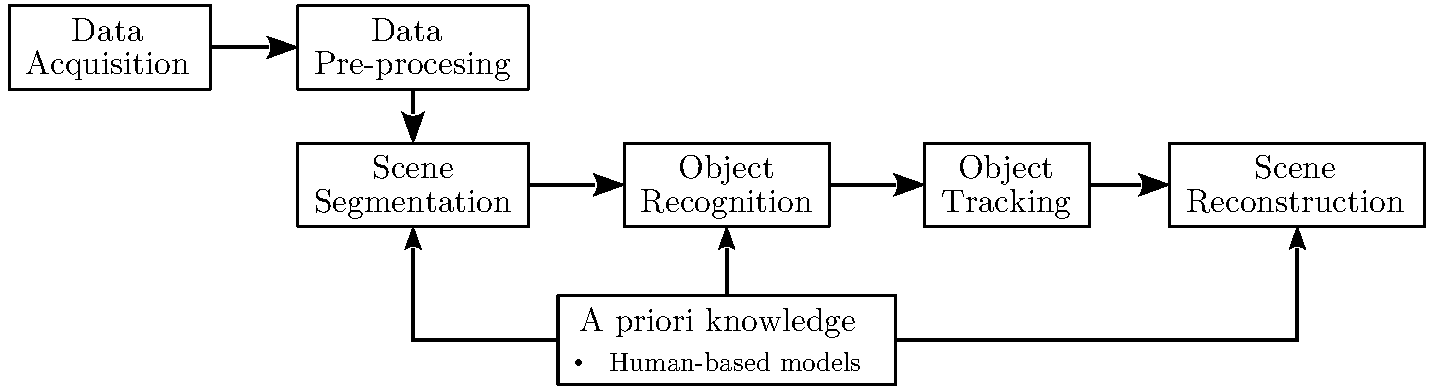
\includegraphics[width=\textwidth]{pipeline_scene_understanding_system}        
    \caption{Typical pipeline of a scene understanding system.}\label{fig:scene_understanding_systme_pipeline}
\end{figure}

Following the pipeline of Fig. \ref{fig:scene_understanding_systme_pipeline}, we can place the tasks of a scene understanding system into five general well-defined computer vision problems.

\begin{enumerate}[label=\roman*]
	\item \textbf{Image pre-processing}, whose objective is to remove the imperfections of an image generated by disturbances such as sensor noise or motion blur. Generally, we perform this task before passing it to a more complex algorithm. Image restoration and inpainting are some examples of this computer vision problem.
	
	\item \textbf{Image segmentation} is the process of partitioning an image into multiple (coherent) segments according to its features and properties. Depending on the application, we can formulate the image segmentation as the problem of classifying pixels with semantic labels (semantic segmentation), or partitioning of individual objects (instance segmentation), or both (panoptic segmentation).
	
	\item \textbf{Recognition} is a classic computer vision problem responsible for determining whether an image contains an object, characteristic, or exercise. Some variants of this problem are the classification, identification, and detection of objects from which many specialized tasks emerge. For example, content-based image search, pose estimation, optical character recognition, reading of 2-d codes, facial recognition, shape recognition, among others.
	
	\item \textbf{Motion analysis} is the problem that searches to estimate the speed of one or more points of interest within an image or 3-d scene by processing a sequence of images. Some examples of this task are egomotion, object tracking, pose estimation, and optical flow.
	
	\item \textbf{Scene reconstruction} is the problem related to the computation of a 3-d model from one or more images of a scene. This model is intended to be a description of the scene as close to reality as possible. 	
\end{enumerate}

These functionalities of computer vision and scene understanding systems are sought in the field of drones. UAVs (or drones) are flying engines that are increasingly present in our lives. We can find them in various sectors, such as the military, commercial or civil, where they can perform very specific tasks. However, in most cases, the development of such applications requires an expert pilot to control the aircraft. 

Commonly, the UAV control is achieved using conventional sensors, such as inertial sensors (IMUs) for orientation and GPS for position. The combination of information coming from these sensors in a flight computer allows the drones to remain stable in the air. However, IMUs present some drawbacks; for example, they suffer from bias error propagation due to the integral drift. On the other hand, the GPS signal is not always guaranteed; for example, the satellite signal may be low or unexisting in urban or indoor environments. A recurrent technique to enhance the drone's position accuracy implies the data fusion of pressure, ultrasonic, radars, and laser range-finders sensors \citep{Tomic.Schmid.ea:IRAM:2012}. The fusion of data can provide the advantages of each sensor. However, a significant limitation of these complex systems is flight time, a parameter mainly linked to the vehicle's total weight and the battery's capacity. Therefore, the use of multiple sensors onboard becomes expensive and impractical.

It is possible to extend the capabilities of a drone by integrating some visual sensor. Contrariwise to other sensors such as Lidars, visual sensors are passive, lightweight, and can acquire valuable information about the surrounding structures, including color and textures, and UAV's self-motion. The addition of visual sensors to perceive the environment has been a recurring strategy that has made these aerial robots more manipulable, safer, and even in some cases, autonomous \citep{He.Qiao.ea:CM:2018}, \citep{Kyrkou.Timotheou.ea:POT:2019}, \citep{Zhu.Wen.ea:arXiv:2020}.That means that the drone can perform a task without the need for human intervention. For this, the drone must be able to move without getting lost; moreover, it must interpret and understand the present scene so that it can be able to detect and avoid potential obstacles on its way. 

Today, one can use different visual sensors, such as monocular cameras \citep{Padhy.Xia.ea:TSC:2018}, stereo cameras \citep{Seitz.Curless.ea:CVPR:2006}, RGB-D cameras \citep{Huang.Bachrach.ea:RobR:2017}, fish-eye cameras \citep{Hrabar.Sukhatme:IROS:2004}, thermal cameras \citep{Gaszczak.Breckon.ea:IRCV:2011}, among others. This wide range of sensors offers more options and flexibility to deal with the problems mentioned above. The integration of such sensors in UAVs has allowed us to see the world from another perspective (literally), and the development of perceptual computer vision algorithms drives the technological improvement of these machines.

We know that today exist applications where vision algorithms have outstripped the capacity of human vision, so they have entirely replaced human personnel, for example, in industrial vision systems tasks, say, the inspection of production lines \citep{Malamas.Petrakis.ea:IVC:2003}. However, in other imaging areas, computer vision systems are only responsible for supplementing specific routines that require a considerable amount of time and experience from human experts. This discrepancy in the vision systems' performance is mainly related to the complexity of the task and the environment's conditions where the task is performed. In industrial vision systems, we can control the working conditions in most cases, while in areas such as robotics and unmanned aircraft (or UAV), with uncontrolled conditions and without large databases, computer vision algorithms bring a real challenge, even though the acquisition system is the same. 

\subsection*{Image Characteristics and Technical Locks in UAV Vision-based Applications}
%\markboth{Introduction}{Problem Statement}
%\section*{Computer Vision Problems in Drone Applications}
 
We can interpret the application and tasks made with drones as missions. Generally, such missions involve three central moments: take-off, navigation, and landing. The drone can perform such stages with conventional sensors; however, visual sensors provide valuable perceptual information about the environment.

Among the three moments that occur in drone missions, navigation and landing are the stages in which visual information (from onboard sensors) and computer vision algorithms most frequently intervene. In the landing stage, the needs and problems can be well-defined since it occurs at the end of the mission. Besides, we can control some conditions by adding pre-designed elements, such as landing targets or landing platforms, to facilitate the task. However, in the navigation stage, computer vision problems are mainly determined by the nature of drone applications.

Drone missions are generally carried out in complex scenes that change as the vehicle moves through space. For example, imagine all the scenarios that a delivery drone goes through during its mission: It can start its route in a commercial area, where the scenes mostly contain warehouses and big open spaces such as parking lots. Then, it could pass through rural areas, where the scenes can contain farmlands or wooded areas. Finally, when the drone reaches the delivery point within an urban zone, the environment may contain houses, trees, electricity, and telecommunications poles, among others. 

The mission through different environments generates considerable lighting changes and shadows, which results in overexposed and (or) dark images. Besides having no control over lighting conditions, we must also consider that the camera's position and orientation vary concerning the scene depending on the vehicle's height and orientation. Moreover, we must also consider the rolling shutter effect present in cameras using CMOS sensors. Therefore, the objects present in the images may have deformations because of the optic and the movement. Figure \ref{fig:img_drone_degradations} shows some images taken with a commercial drone in a natural setting. We can observe how the environment's lighting conditions and the nature of aerial applications introduce deformations to the images and objects present in the scene. 

Finally, we must not forget that we acquire the input images from an onboard camera, which is generally not stabilized; therefore, the images may be noisy or blurry. Such problems limit a computer vision algorithm to be globally efficient in all or most situations.


\begin{figure}[!ht]
    \centering
    \begin{subfigure}[b]{0.38\textwidth}
        \frame{\includegraphics[width=\textwidth]{Bebop_A}}
        \caption{Presence of shadows}
    \end{subfigure}
        ~ %add desired spacing between images, e. g. ~, \quad, \qquad, \hfill etc. 
      %(or a blank line to force the subfigure onto a new line)
    \begin{subfigure}[b]{0.38\textwidth}
        \frame{\includegraphics[width=\textwidth]{Bebop_B}}
        \caption{Saturations}
    \end{subfigure}
        ~ %add desired spacing between images, e. g. ~, \quad, \qquad, \hfill etc. 
      %(or a blank line to force the subfigure onto a new line)
    \begin{subfigure}[b]{0.38\textwidth}
        \frame{\includegraphics[width=\textwidth]{Bebop_C}}
        \caption{Change of scale}
    \end{subfigure} 
    \caption{Some examples of image degradations present in aerial imaging and UAV applications.}\label{fig:img_drone_degradations}
\end{figure}

In addition to the problems related to the complex scene conditions, we must consider that a drone is subject to sudden changes in the environment, such as wind gusts, which can affect its stability and modify the visual information given by the onboard sensors. In such cases, the vision algorithms for drone navigation must process the input information fast enough to provide answers and transform them into real-time decision actions.

Considering the conditions and problems of vision-based drone applications, we argue that a system for scene understanding is necessary for this kind of application. Moreover, scene understanding must use low-level information such as intensity, color, and texture in combination with perceptual tools to generate a robust image interpretation to the characteristic visual conditions of the aerial platforms. Among these classic computer vision problems, image segmentation is a crucial stage in the scene understanding pipeline. Image segmentation is a low-level task; however, it is critical for high-level applications such as classification, object tracking, reconstruction, and scene understanding. A robust segmentation to the changes and variants of complex environments allows the generalization of high-level tasks to new contexts and applications.

\section*{Image Segmentation State of the Art}
\markboth{Introduction}{Perceptual Information and Image Segmentation State of the Art}

Image segmentation has a long history in computer vision and is present in many applications in medicine, biology, robotics, and physics. Here, we present a brief review of the state-of-the-art segmentation methods taking into account the approach used and relationship with vision perception (a more detailed version of the state-of-the-art of segmentation methods appears in chapter \ref{ch:perceptual_object_boundaries_detection}, section \ref{sec:SoA_segmentation_methods}). For this purpose, we divide the image segmentation techniques into classical methods and Artificial Intelligence (AI) methods. 
%\cite{Khan:IJIG:2013}

\subsubsection*{Classical Image Segmentation Techniques} 
Classical image segmentation methods can be organized into two groups: those that identify similarities or those that identify discontinuities \citep{Zaitoun.Aqel:ICCMIT:2015}. The first kind of approach detects similar pixels in the image based on some specific threshold or criteria for split-merge and growing regions. The second category of methods tries to find the boundaries between dissimilar pixels in the image. A more specific classification according to the technique used divides segmentation methods into Threshold-based, edge-based, region-based, watershed-based, clustering-based, PDE-based, and Graph-based \citep{Zaitoun.Aqel:ICCMIT:2015}.

\textbf{Threshold-based} algorithms are one of the simplest image segmentation techniques. The threshold operation divides the image by comparing the intensity of the pixels to a specific threshold value\citep{Sezgin.Sankur:EI:2010}. This kind of method can only segment images into background and foreground based mainly on the intensity pixel information. This property is convenient when there is a significant contrast difference between the objects and the background. The major challenge of such approaches is the choice of the threshold value. The simplest option is to use a global threshold for the whole image; however, this option fails when the illumination in the image is uneven. Local thresholding methods solve this problem by proposing multiple thresholds \citep{Niblack:ImageProcc:1986}, \citep{Sauvola.Pietikainen:ICPR:2000}; however, the computation time can increase considerably. One of the most popular approaches in this category that automatically determine the threshold value is Otsu's method \citep{Otsu:SMC:1979}.

The \textbf{Edge-based} segmentation methods attempt to solve the image segmentation problem by detecting edges in an image according to the differences in texture, contrast, grey level, color, saturation, and other properties \citep{Saini.Arora:IJICT:2014}. Some of the more well-known methods in this category employ operators that use the first and second derivatives of the image to identify abrupt changes in the intensity of the image, for example, the Sobel \citep{Sobel.Feldman:SAIL:1990}, Roberts \citep{Roberts:Thesis:1963}, Gradient \citep{Maitre:Book:2003}, Prewitt \citep{Prewitt:PPP:1970}, and Laplacian \citep{Marr.Hildreth:PRS:1980} operators. On the other hand, one of the state-of-the-art reference work is the Probability-boundary (Pb) \citep{Malik.Belongie.ea:IJCV:2001},  which uses the intensity and color, and texture information to obtain the edges of the image. 

The \textbf{Region-based} segmentation methods partition the image into similar regions according to predefined criteria. Depending on the strategy used to arrive at the final segmentation, they can be organized into region growing and splitting and merging techniques \citep{Sezgin.Sankur:EI:2010}. Region growing techniques define a group of seed pixels from which regions start to grow \citep{Zucker:CGIP:1976, Adams.Bischof:TPAMI:1994}. Regions grow by appending to each seed pixel those neighboring pixels that have predefined properties similar to those of the seed pixels (e.g., intensity or color). Regions stop growing when they reach a particular predefined stop criterion (e.g., size or shape of the region).
Conversely, splitting and merging techniques do not require seed pixels. This technique successively divides the image into quadrants based on a homogeneity criterion, then similar regions are merged to form the final segmentation. This strategy includes the quad-tree data structure \citep{Horowitz.Pavlidis:ACM:1976}, which means a parent-child node relationship.
In practical applications, the region growing and splitting and merging algorithms are usually used in combination \citep{Ikonomatakis.Plataniotis.ea:ICDSP:1997}. This combination is more effective for the segmentation of complex scenes defined by some complex objects or the segmentation of certain natural scenes, such as image segmentation with insufficient prior knowledge.

The \textbf{Watershed-based} segmentation is a technique that utilizes image morphology and combines the characteristics of edge- and region-based methods described above. First, this method computes the gradient of an image. We can see this gradient as a map that reflects the topography of the image through the intensity values of the pixels. Then, segmenting an image is equivalent to flooding the topography from a group of seed pixels, where the edges of the image appear as the highest ridges where the flood water meets \citep{Meyer.Beucher:JVCIR:1990, Beucher.Meyer:Book:1993}. The watershed method is strictly linked to hierarchical segmentation methods \citep{Najman.Schmitt:PAMI:1996}. This feature of hierarchical dependence complexifies the efficient implementation in embedded processors. Many strategies introduce other definitions of the watershed transform to solve the complexity problem,  which simplifies and accelerates its computation \citep{Roerdink.Meijster:IOS:2000} , \citep{Dejnozkova.Dokladal:ICASSP:2003}, \citep{Chabardes.Dokladal.ea:ICIP:2016}.

Another alternative to obtain the segmentation of an image is by using clustering methods. The \textbf{clustering-based segmentation} methods are unsupervised techniques that classify the image pixels into clusters (disjoint groups) with similar features. The objective of pixel clustering is to maximize intra-class differences and minimize intra-class differences; that is, the pixels in each class should be as similar as possible, and those in the different groups should be as different as possible \citep{Steinley:BJMSP:2006}. The k-means technique is known as a hard-clustering technique since each pixel can belong only to one class. Fuzzy algorithms (soft-clustering) relax that condition, and each data point can belong to more than one cluster. This behavior is suitable in applications where there are no crisp boundaries between objects, such as tissue classification \citep{Caldairou.Passat.ea:PR:2011} and tumor detection \citep{Preetha.Suresh:CCT:2014}. Among the soft-clustering methods, fuzzy C-means clustering \citep{Dunn:JC:1973} is one of the most used.

\textbf{PDE-based} segmentation methods use Partial Differential Equations to model the image contours and obtain an image segmentation.  Active Contour Model (or Snakes) transform the segmentation problem into
PDE. Some famous methods of PDE used for image
segmentation are Snakes \citep{Kass.Witkin.ea:JCV:1988}, Level-Set \citep{Osher.Sethian:JCP:1988}, Fast Marching \citep{Forcadel.LeGuyader.ea:NA:2008}, and Mumford Shah method \citep{Mumford.Shah:CPAM:1989}. One of the main problems of these methods is the high computational time for the resolution of the PDE, which limits its use on embedded platforms. This limitation has been addressed in the implementation level through architectures that allow multi-core parallel calculation \citep{Dejnozkova.Dokladal:ICVIE:2003, Dejnozkova.Dokladal:ICASSP:2004}.

The last group of classical methods for image segmentation is \textbf{Graph-based}. These methods make use of graph theory to represent the image as a graph.  Typically, a pixel or a group of pixels are associated with nodes, and the edge weights define the affinity between neighboring pixels. Then, we can partition the graph according to a criterion designed to model good clusters. Each resulting partition of nodes is considered a segmented object in the image. Some popular algorithms in this category are normalized cuts \citep{JianboShi.Malik:PAMI:2000}, random walker \citep{Grady:PAMI:2006}, minimum cut \citep{Wu.Leahy:PAMI:1993}, isoperimetric partitioning \citep{Grady.Schwartz:PAMI:2006}, and minimum spanning tree \citep{Zahn:TC:1971}. Some of the segmentation methods can combine strategies. For example, spectral clustering \citep{Ng.Jordan.ea:NIPS:2001} uses the graph theory and the similarity of the graph edges to cluster the image pixels into coherent regions. On the other hand, \citep{Cousty.Bertrand.ea:PAMI:2009} define the watershed cuts cut on edge-weighted graphs using the Minimum Spanning Forest.

This group of approaches and techniques (known as classical, conventional, or traditional) can use structural, stochastic, or hybrid techniques to segment an image. Structural techniques require structural data from the image, such as distributions, histograms, pixel density, or color distribution. Stochastic techniques require information about the discrete values of the pixels. Machine learning methods, such as the clustering techniques, fall into this category. Finally, hybrid techniques may use structural information of image regions and the discrete values of the pixels of the whole image for the segmentation. The choice of the method to segment an image depends on the type of image and the type of segmentation that we seek to obtain (for example, over-segmentation or segmentation to pixel precision). Regardless of this, we consider it essential to consider the perceptual elements of the data to achieve a meaningful interpretation of the scene.

\subsubsection*{AI Image Segmentation Techniques} 
The \textbf{Artificial Neural Networks- (ANN) based} techniques (a.k.a. Deep Learning (DL) techniques) are probably the most widely used methods today because of their efficiency and accuracy. They are part of the supervised techniques, i.e., they require an annotated database for training, validation, and testing. In ANN-based methods, every neuron corresponds to the pixel of an image, which means the image is mapped to the neural network. Then, the image in the form of the neural network is trained using labeled data to find the connection between neurons (pixels). Lastly, the new images are segmented from the trained model. 

In recent years, neural network techniques (also known as deep learning (DL) techniques) have led to new models for image segmentation. We can classify these methods roughly according to the architecture they use. Convolutional Neural Networks  (CNNs) are among the most widely used and successful architectures in computer vision. This model, initially proposed by \cite{Fukushima:BC:1980}, is inspired by the model of the human visual cortex. Generally, CNNs contain convolution layers, non-linear layers (or activation functions) for feature mapping and pooling layers. Some of the best-known CNNs in the literature include LeNet \citep{Lecun.Bottou.ea::1998}, AlexNet \citep{Krizhevsky.Sutskever.ea:NIPS:2012}, VGGNet \citep{Simonyan.Zisserman:arXiv:2015} and ResNet \citep{He.Zhang.ea:ICVPR:2016}. 

Due to their characteristics, CNNs require dense layers and a large number of parameters, which makes them highly expensive. Fully Convolutional Networks (FCN) \citep{Long.Shelhamer.ea:CVPR:2015} solve this drawback by stacking several convolution Layers with similar padding to preserve the dimension and output a final segmentation map of the same size as the input image. Some of the best-known models are VGG16 and GoogleNet \citep{Szegedy.Liu.ea:arXiv:2014}.

Other deep learning backbones are the Encoder-Decoder and Auto-Encoder architectures. This type of model is known as two-stage networks. The first stage, encoding, compresses the input information into a space-latent representation, while the second stage, decoding, predicts an output from the representation. Some examples of networks that follow this architecture are DeConvNet \citep{Noh.Hong.ea:ICCV:2015}, SegNet \citep{Badrinarayanan.Kendall.ea:PAMI:2017}, U-Net \citep{Ronneberger.Fischer.ea:MICCAI:2015}, W-net \citep{Xia.Kulis:arXiv:2017}, Linknet \citep{Chaurasia.Culurciello:VCIP:2017}, among others.

Object detection and image segmentation are complementary tasks in computer vision. Similarly, exist architectures designed for object detection, such as Regional CNN (R-CNN), which have been successfully adapted for image segmentation. Some examples are the Faster R-CNN \citep{Ren.He.ea:PAMI:2017}, Mask R-CNN \citep{He.Gkioxari.ea:PAMI:2020} and Masklab \citep{Chen.Hermans.ea:CVPR:2018} architectures. The operation principle of these architectures is to extract the features of certain regions of interest to infer the class and the coordinates of the bounding box of the object.

A very recent family of architectures are those based on Generative Adversarial Networks (GANs) \citep{Goodfellow.Pouget-Abadie.ea:NIPS:2014}. This architecture consists of two networks, a generator, and a discriminator. The generator has the task of reproducing distributions similar to the real samples. On the other hand, the task of the discriminator is to distinguish the fakes samples from the real ones. GANs models include Convolutional-GANs \citep{Radford.Metz.ea:arXiv:2016}, Conditional-GANs \citep{Mirza.Osindero:arXiv:2014}, and Wasserstein-GANs \citep{Arjovsky.Chintala.ea:arXiv:2017}.

Other popular DL architectures for image segmentation include Feature Pyramidal Networks (FPN) \citep{Lin.Dollar.ea:CVPR:2017}, which takes a multi-scale approach, or hybrid ones that combine classical methods such as the Active Contour Model \citep{Kass.Witkin.ea:JCV:1988} and CNNs, or the watershed transform in the deep watershed architecture \citep{Bai.Urtasun:CVPR:2017}. 

The literature on methods based on DL architectures for image segmentation is vast. For a more detailed survey of the state of the art of ANN-based methods for image segmentation, please check \citep{Sultana.Sufian.ea:KBS:2020} and \citep{Minaee.Boykov.ea:PAMI:2021}.

%\citep{Kelm.Rao.ea:CAIP:2019}
AI-based image segmentation methods are experiencing popularity and growth that has benefited from advancements in computing power and the recent creation of publicly accessible annotated databases. However, its use in particular applications where there are not (yet) large enough annotated databases is complicated. Furthermore, despite the performance in challenging benchmarks, in many cases, the interpretability of the results of these methods remains open questions.

\subsubsection*{Vision-based UAV Navigation Related Works}
In the literature, we can find many works that deal with computer vision for drone navigation. The different approaches are strongly related and motivated by the application's aim and the conditions in which the task is developed. We can differentiate two main vision-based techniques for UAV navigation; 1) localization and mapping and 2) obstacle avoidance.

Simultaneous Localization and Mapping (SLAM) falls within the first group techniques, where drone navigation is a consistent result. This technique estimates the drone's local pose and builds a 3-d model of its surroundings employing visual sensors. Visual Odometry (VO) \citep{Scaramuzza.Fraundorfer:RAM:2011} is responsible for the robot motion estimation while the maps are built with occupancy grid algorithms \citep{Thrun.Bu:AI:1996}. According to the image information used to perform a SLAM, we can classify these approaches into feature-based methods, which extract a set of image features (e.g., lines, points) in a sequence of images, and direct-based methods, which make use of the image intensity information to estimate the structure and the motion of the robot \citep{Taketomi.Uchiyama.ea:TCVA:2017}. The importance of a correct segmentation of the image is that we can also create a depth chart of the scene from it and consequently achieve the visual odometry \citep{Drouyer:Thesis:2017, Drouyer.Beucher.ea:MMASP:2017}. 

The use of SLAM techniques for UAV navigation presents remarkable advantages. Feature-based methods can use various feature detectors, which typically count with an optimization stage to produce fast algorithms. Direct-based methods have the advantage of being robust to image degradations; they can lead better with images with texture and blurred zones; besides, the map produced is of an acceptable resolution. Interestingly, the strengths of the first group of methods are the weak points of the second and vice versa. A method that tries to gather the benefits of both approaches is the Semi-direct Visual Odometry \citep{Forster.Pizzoli.ea:ICRA:2014}; however, in general, the state-of-the-art SLAM methods is more mature in the autonomous vehicle environment \citep{Singandhupe.La:IRC:2019}.

There are approaches for drone navigation that, in parallel to SLAM, favor the avoidance of obstacles. This capability is essential for achieving free collision missions in both indoor and outdoor environments. A recurrent solution, as we early mentioned, is the multi-sensor data fusion. \cite{Gageik.Benz.ea:ACCESS:2015} present a platform using low-cost ultrasound and IR sensors; however, despite the obtained results, it utilizes several sensors to retrieve environment information, and yet, it does not get a perceptual representation of the scene due to the low resolution and perceptive capacity of the sensors. On the other hand, vision-based techniques for obstacle avoidance could detect obstacles and, in some cases, recognize and classify the object representing the obstacle \citep{Li.Ye.ea:IROS:2016}. 

We can classify the visual methods for avoidance of obstacles into two groups. The first, SLAM-based techniques, make use of the principles stated above. The 3-d reconstruction provides accurate and sophisticated maps and allows the air vehicle to travel with more information about the environment. In \citep{Moreno-Armendariz.Calvo:ICMEAE:2014}, takes this advantage to develop an obstacle avoidance approach for static and dynamic obstacles. The second group is the flow-based methods which historically, were inspired by the navigation of insects such as bees \citep{Srinivasan.Gregory:PTBS:1992} or flies \citep{Franceschini.Ruffier.ea:InTech:2009}. Many insects in the wild identify obstacles through the intensity of light. During the flight, their eyes produce an optical flow that provides accurate spatial information. Currently, there are also works inspired by the behavior of the human eye \citep{Al-Kaff.Meng.ea:IVS:2016}. The technique measures the object size from the idea that objects in the robot's vision field are more significant as the obstacle is close.

In general cases, obstacle avoidance techniques are strongly linked to the camera parameters and acquisition conditions. The algorithms are often fine-tuned. Given the condition, a drone operates in an environment without prior knowledge and under uncontrolled conditions. Hence some more general, unsupervised methods are needed.

Today, the most efficient algorithms are those based on Neural Network (NN) architectures and supervised learning techniques. Nevertheless, these techniques have remarkable disadvantages that question their usability and applicability in real-life drone missions \citep{Treboux.Genoud.ea:IWBIS:2018}. From a practical and even economic point of view, there is a limit to the number of applications in which we can use supervised methods given the fact that we need a lot of annotated data \citep{Xu.Wang.ea:CEA:2020}. The collection and the correct labeling of data representing a problem are valid only for a small number of applications.

The need for abundant information comes with high computational times required for model learning, ranging from a couple of hours to weeks. Of course, we can minimize this variable by increasing our machines' computing power; however, today, only those with large computing infrastructures can afford to train models with hundreds of billions of parameters.  

The above statement introduces the next disadvantage of deep neural network-based learning models: hyperparameters. We can roughly divide hyperparameters into two categories: 1) optimizer hyperparameters, which include the learning rate, the batch size, and the number of epochs, and 2) model-specific hyperparameters, which include the number of hidden layers, the first hidden layer, and the number of layers. Choosing the appropriate hyperparameters plays a crucial role in the success of neural network architectures because they control the learning algorithm's behavior, define the network structure, and define how the network is trained. Although there are methods to optimize their choice, generally, this task is a heuristic process, and their fine-tuning is a function of the specific application. It is possible to follow some rules based on experience, copy the same values from some other problem or make the setting by trial and error, though we cannot know the best value for a hyperparameter.

We can thus conclude that it is crucial to have the means to understand the scene, depending less on the parameters fixed in advance or the data sets prepared for a particular mission. In the following paragraphs, we present the contribution of this thesis to this issue.


%Nowadays, there is a wide variety of image segmentation techniques, some considered general-purpose and some designed for specific images.  On the other hand, \cite{Zaitoun.Aqel:ICCMIT:2015} propose a two-group classification: layer-based and block-based segmentation methods. Under these two taxonomies, we focus on classical or block-based segmentation methods. More specifically, we perform region-based segmentation and boundary-based segmentations.

\section*{Scope of the Thesis}
\markboth{Introduction}{Scope of the Thesis}
%First of all, this thesis work is motivated mainly by my profile and interests in robotics and control theory, specifically in air vehicles. 

The interaction between computer vision and applications made with unmanned aerial vehicles is extensive. This collaboration has generated new methodologies and approaches, both theoretical and practical, but has also given way to new research questions. 


Knowing the fundamental limitations of aerial robots and the complexity of drone applications, we explore computer vision theory to propose algorithms that improve and provide assistance in drone navigation tasks. In this sense, we are interested in studying the scene's perceptual information for their treatment and interpretation.

We focus primarily on the vision processing problems: object segmentation and recognition. We argue that two computer vision tasks are crucial for image understanding and have to be carefully treated in complex, uncontrolled environments. From this perspective, we focus on using low-level image features to extract perceptual information. 

Based on Fig. \ref{fig:scene_understanding_systme_pipeline} and considering the scope of the work in this thesis, we propose a new pipeline for scene understanding systems. In this new pipeline, the pre-processing of the image involves its perceptual decomposition, while the segmentation stage considers the perceptual elements of the image. The proposed pipeline for scene understanding is showed in Fig. \ref{fig:my_scene_understanding_systme_pipeline}. The peculiarity of this pipeline is that it eliminates the dependency on the a priori models, at least for the tasks of segmentation and image recognition (tasks that we study in this thesis). 

\begin{figure}[!ht]
    \centering
    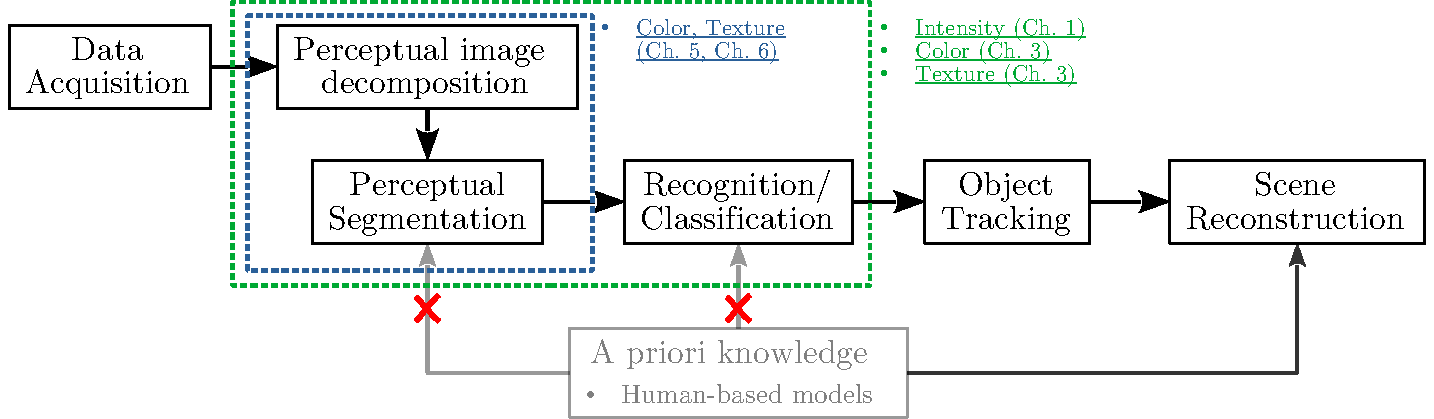
\includegraphics[width=\textwidth]{my_pipeline_scene_understanding_system}        
    \caption{Proposed pipeline of a scene understanding system.}\label{fig:my_scene_understanding_systme_pipeline}
\end{figure}

Throughout this work, we develop algorithms that are capable of handling a variety of real-world conditions. All these algorithms aim to segment the physical objects that we, as humans, define as perceptually interesting. For this purpose, we use intensity, color, and texture image information to extract low-level primitives, such as contours. In Fig. \ref{fig:my_scene_understanding_systme_pipeline}, we show the stages of scene understanding that we study in this thesis and the low-level primitives involved in the task: in green, the recognition and classification of objects use intensity, color, and texture, and in blue, the perceptual segmentation uses color, texture and the relationship between them. We use these primitives in conjunction with statistical and geometric tools from computer vision and signal theory, such as anomaly detector, optimal transport, and Gabor functions. Instead of using supervised methods, we focus on decomposing the image information from the point of view of signal theory and physics to use it later on non-supervised or mathematical morphology methods.
%So it is worth mentioning that the practical aspect linked to the implementation and the generation of solutions in real-time are not a priority. The developed algorithms provide solutions to the recognition and scene understanding problem's variants, such as the classification, identification, and detection of objects from a qualitative point of view, always looking for the application's physical meaning. 

Regarding the nature of the input data, we use only gray-level or color images as input information, favoring monocular cameras among the wide range of visual sensors reviewed previously. This choice allows replicating the algorithms with low-cost cameras that can be easily embedded in a drone.

%One last point about the focus of this work is about the type of computer vision techniques. The algorithms proposed in this thesis are based on traditional computer vision techniques, that is, non-deep learning techniques. This decision is consistent with drone applications' nature, where there are not necessarily rich enough annotated databases to apply the most sophisticated artificial intelligence models.

\section*{Contributions of the Thesis}\label{sec:objectives_of_the_thesis}
\markboth{Introduction}{Contributions of the Thesis}

%In this Ph.D. thesis, we aim to develop general computer vision algorithms considering the challenges and needs of UAV navigation. 

The primary objective of this Ph.D. thesis is to propose a new methodological framework for decomposing images before segmenting and detecting objects in the context of the scene understanding. The idea is to apply this methodological framework to assist in control and decision-making in drone navigation tasks. Therefore, the framework must be robust to image degradations existing in environments with uncontrolled conditions, in addition to being independent of the choice of specific parameters for its operation.

%During the thesis, we consider many specific drone tasks, such as:
%
%\begin{enumerate}[label=\roman*]
%	\item \textbf{Recognition} is a classic computer vision problem responsible for determining whether an image contains an object, characteristic, or exercise. Some variants of this problem are the classification, identification, and detection of objects from which many specialized tasks emerge. For example, content-based image search, pose estimation, optical character recognition, reading of 2-d codes, facial recognition, shape recognition, among others.
%	\item Environment awareness.
%	\item Detection and avoidance of obstacles.
%	\item Identification and following of targets.
%\end{enumerate}
%Given these tasks, the work focuses on the scene understanding problem. To deal with this problem, 
We extend the study of primary image information such as intensity, color, texture, and texture color and low-level image primitives such as contours. Therefore, some secondary objectives involve building a representation of the image in feature space using concepts from signal theory, geometry, and statistics, in addition to concepts from human perception. We seek to validate the proposed image representation using unsupervised approaches in real applications following traditional machine learning and segmentation algorithms.

Figure \ref{fig:general_diagram_framework} shows a general flowchart of the contributions of this thesis. The first stage of the flowchart shows low-level information and the methods we use to extract it; here, we work with intensity, color, texture, and the relationship between color and texture. The second stage of the diagram shows the different representations of the image obtained from the perceptual information contained in the primitives. Finally, the diagram's third section collects the different applications used to validate the image's feature spaces constructed in this thesis. Although the idea of a single framework itself is an ambitious goal, in this thesis, we present several algorithms that apply the proposed methodology with one or more features to solve different computer vision problems such as object detection and recognition, image retrieval systems, perceptual object boundaries detection, and image segmentation.

The interest of obtaining a representative space of the image information from low-level hand-made features lies in the possibility of using it in a semi-supervised pipeline. By injecting annotated information into the frame, it might make generalizations and obtain medium- or high-level features such as the importance of color and texture information to a human when segmenting an image. 

\begin{figure}[!ht]
    \centering
    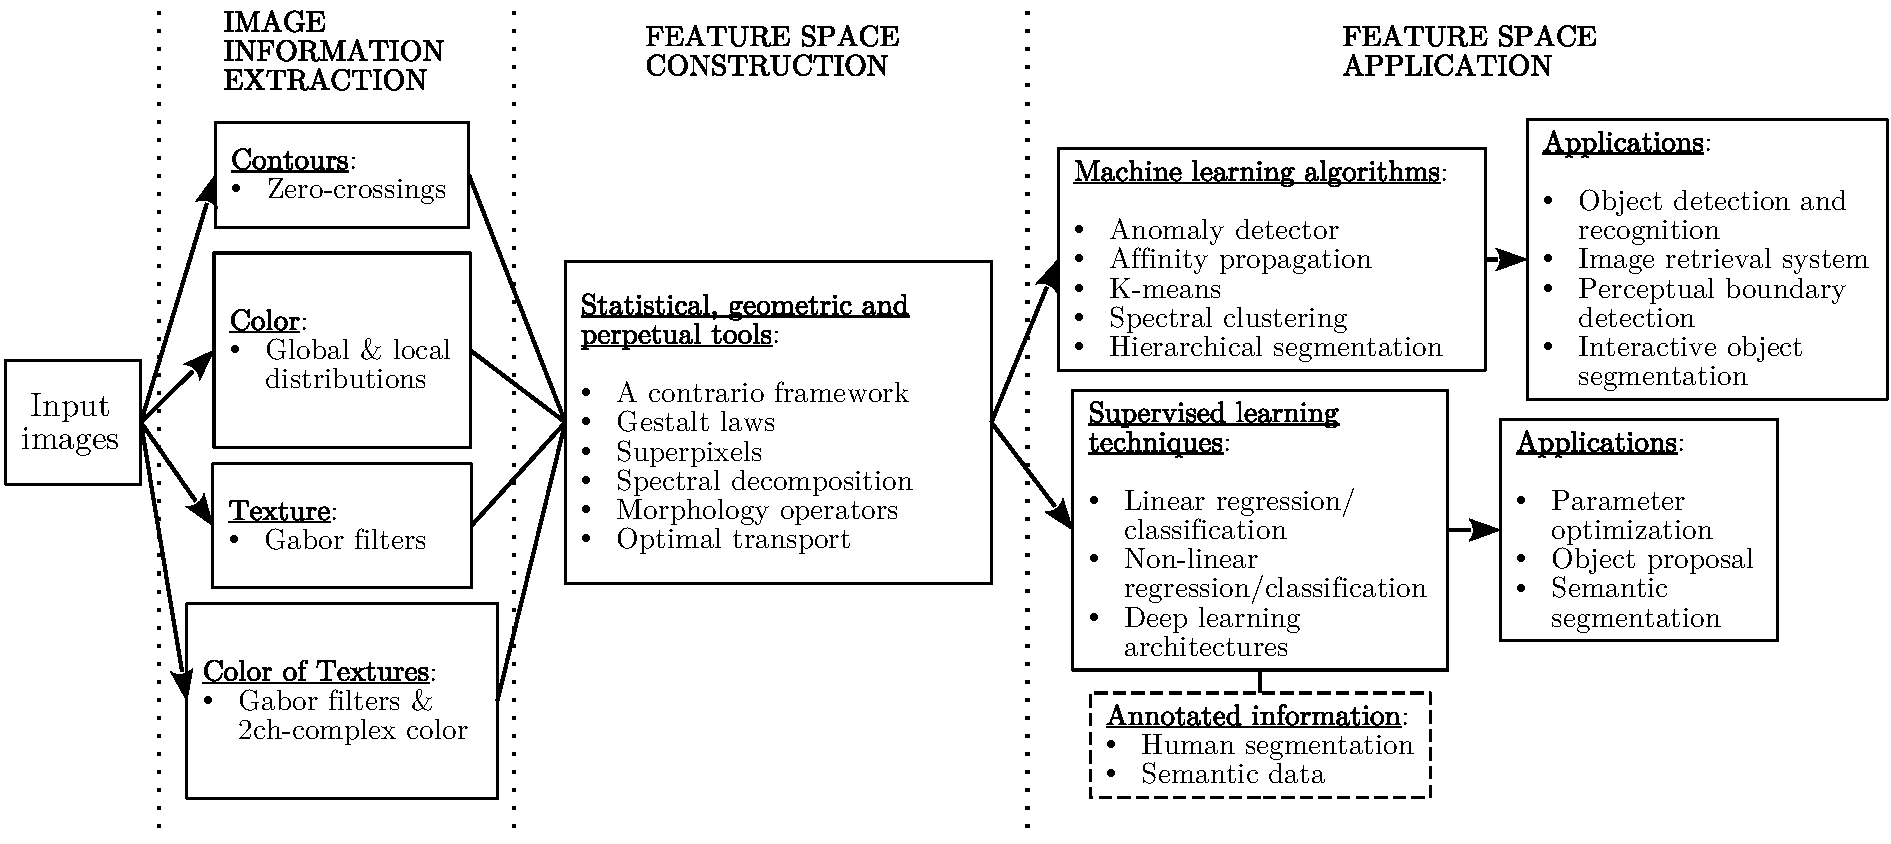
\includegraphics[width=\textwidth]{general_framework_diagram}        
    \caption{Flowchart of thesis contributions.}\label{fig:general_diagram_framework}
\end{figure}

Specifically, the contributions of this thesis include:

\begin{itemize}
	\item A novel non-parametric framework for fully unsupervised object detection robust to the image degradations present in complex, uncontrolled environments (chapter \ref{ch:landing_target_detection}).
	\item A qualitative and quantitative study between the most popular measures in the comparison of distributions (chapter \ref{ch:similarity_measures}). 
	\item An unsupervised image retrieval system based on global color/texture information (chapter \ref{ch:similarity_measures}).
	\item Extensive analysis of Gabor filters and their properties in the space-frequency domains (chapter \ref{ch:spectral_image_decomposition}).
	\item Generation of a feature space that includes the color and texture information of an image (chapter \ref{ch:complex_spectral_image_decomposition}).
	\item Unsupervised framework for natural image segmentation (chapter \ref{ch:perceptual_object_boundaries_detection}).
\end{itemize}

Finally, this thesis aims to show that traditional computer vision methods are (still) a reliable option to develop object detection and recognition for relatively complex tasks. We place this argument in the current context of computer vision, where there are hundreds of algorithms based on Neural Networks and Artificial Intelligence. Besides the NN and AI algorithms for image segmentation and object detection are highly performant, they lack a physical (and in many cases logical and argued) interpretation of its results. Furthermore, these algorithms are in trouble when it comes to image analysis of complex scenarios or applications where there is no database rich enough to do the learning process.


\section*{Organization of the Document}
\markboth{Introduction}{Organization of the Document}

To communicate our proposal and the objectives mentioned above in a clear and structured way, we present a thematic and chapter organization of the document. The thematic organization follows, to some extent, the complexity of the three low-level image information we used during this thesis: intensity, color, and texture. Then, we can identify three main parts in this thesis.

\begin{enumerate}
	\item The first part is dedicated to studying the intensity information of the image, in which we review in detail some of the classic methods for obtaining image contours. We use this information in conjunction with the \textit{a contrario} method and the Gestalt organizing laws to detect and identify landing targets. This part includes chapter \ref{ch:landing_target_detection}. 
	\item The second part main topic is studying the properties of color and texture of an image. We are interested in the global distribution of this information and the existing metrics to measure the similarity between the distributions; we apply and validate these concepts in two image retrieval systems. This part covers from chapter \ref{ch:color_texure_representations} to chapter \ref{ch:spectral_image_decomposition}.
	\item The third part extends the study of color and texture in images, exploding the local distribution of these primitives and studying the influence of color information on the generation of textures in an image. We propose a multi-spectral image decomposition helpful on the object segmentation tasks using classic clustering algorithms and for the generation of high-level texture features. Moreover, we propose a completely unsupervised framework for the detection of perceptual boundaries. We also explore different strategies to obtain the segmentation of natural images using the obtained perceptual boundaries. This part includes chapter \ref{ch:complex_spectral_image_decomposition} to chapter \ref{ch:perceptual_object_boundaries_detection}.
\end{enumerate}

The organization by chapters is structured as follows:

\begin{itemize}
	\item \textbf{Chapter \ref{ch:landing_target_detection}} addresses the bases of the Gestalt theory, including the grouping laws and the Helmholtz principle. We formalize these concepts of human perception mathematically and formulate a non-parametric algorithm that follows an unsupervised framework based on an image's contours. We use the developed framework in the autonomous drone landing problem, specifically detecting and identifying landing targets.  The chapter also presents a review and a quantitative comparison of different traditional methods for extracting image contours.
	
	\item \textbf{Chapter \ref{ch:color_texure_representations}} presents a detailed review of the different ways to represent the color and texture information in an image. The chapter contains a review of various color spaces and their main properties and an introduction to the different techniques for characterizing textures in the literature. Such information is of relevant importance in constructing the framework and the approaches to measure similarity between distributions.
	
	\item \textbf{Chapter \ref{ch:similarity_measures}} presents the analysis between different similarity measures between distributions, showing the advantages and disadvantages of each of them. In particular, we focus on the theory of optimal transport through the Earth Mover's Distance. We show the advantages of this metric over traditional similarity measures using an image retrieval system based on an image's global color and texture information.
	
	\item \textbf{Chapter \ref{ch:spectral_image_decomposition}} explores the physical and human perception aspects of Gabor's filters. We show the steps involved in designing an optimized and efficient Gabor family of filters. The proposed filter family models and captures the texture information through an energy-efficient decomposition of the image. Such spectral decomposition of the image deals with Heisenberg's uncertainty principle. The chapter presents the description of parameters that allow complete customization of the filter family according to the application.
	
	\item \textbf{Chapter \ref{ch:complex_spectral_image_decomposition}} brings an analysis of the texture information present in color images, showing the strong relationship between those two features. Using the spectral analysis of an image with the previously defined Gabor filters, we generate a feature space that simultaneously captures the color and texture information. We show the richness of such feature space by performing unsupervised image segmentation only using simple clustering techniques. Moreover, we show some novel high-level texture features resulting from the spectral image decomposition.
	
	\item \textbf{Chapter \ref{ch:perceptual_object_boundaries_detection}} introduces a framework for detecting perceptual boundaries of objects present in natural images. This framework brings together concepts addressed in this document, such as the spectral decomposition of images, the optimal transport as a true metric, and the relationship between color and texture information. Besides, using the hierarchical segmentation technique, we segment natural images in an unsupervised manner. We perform a quantitative and qualitative validation of our method using a known database.
	
%	\item \textbf{Chapter \ref{ch:general_conclusion}} contains the general conclusions of the thesis and addresses the different possible research lines as a continuation of this work.
	
\end{itemize}


%    \afterpage{\blankpage}
	\cleardoublepage

%	% created on 28/07/2020
% @author : ebazan
\part{Global Color and Texture}\label{part:global_color_texture}%Image Global Color and Texture

\section*{Introduction}
In part \ref{part:image_contours}, we show that low-level features, such as image contours, provide useful perceptual information that can be used to solve complex problems. We presented a framework that uses the concepts of human perception and contour information for the unsupervised detection of landing targets. This framework is able to identify the marker under degraded operating conditions using only exogenous features from the contours, which are identified on gray-level images. The framework can be improved by adding other features that provide perceptual information of a scene.

In this part of the thesis, we review two more low-level image features: color and texture. Both features are widely involved in the perceptual process of humans and their study can be very extensive. The objective of this part is to explore the image color and texture features for their future integration into a general framework for object detection. Particularly, in this part of the thesis we are interested in the global distribution of color and texture information of an image. For this purpose, the chapter that opens this part seeks to remember recall the definition of color and texture in the field of computer vision. Moreover, it review different approaches to color representation as well as different strategies for characterizing texture features. Later, in chapter \ref{ch:similarity_measures}, we take interest at the comparison of distributions, particularly in the study of the Optimal Transport (OT) as a metric for the measurement of similarity between distributions and its application in the field of computer vision.

Throughout these chapters of the thesis, we address the study of those two properties using simple images containing the information of interest; in the case of color, images containing low color variation and; in the case of texture, grayscale images with homogeneous textures.

The main contributions of this part are:

\begin{enumerate}
	\item Review of the state of the art of global color representations and texture characterizations.
	\item Review of the state of the art of similarity measures, particulary the interpretation of the OT in computer vision: the Earth Mover's Distance (EMD).
	\item Qualitative and quantitative study between the most popular measures in the comparison of distributions and the EMD. 
	\item An unsupervised image retrieval system based on global color/texture information.
\end{enumerate}


\chapter{Global Representations of Color and Texture } \label{ch:color_texure_representations}

\section*{Résumé}
\noindent 
Ce chapitre présente une compilation des différentes manières de représenter les informations de couleur et de texture présentes dans une image. En ce qui concerne les informations de couleur, nous introduisons certains types d'espaces colorimétriques et leurs origines. De plus, nous présentons quelques techniques pour synthétiser ces informations. Dans le cas de la texture, nous présentons les différentes méthodologies pour son étude, en mettant en évidence les avantages et les inconvénients de chaque méthode.
\section*{Abstract}
\noindent 
This chapter presents a compilation of the different ways of representing the color and texture information present in an image. When it comes to color information, we present some of the most popular color spaces used as well as their origins and relationship to human perception. In addition, we present some techniques to synthesize this information. In the case of texture, we present the different methodologies for its study, highlighting the advantages and disadvantages of each method. The information presented in this chapter serves as the basis for the next chapter.

\section{Introduction}

If we look around us, we can see that many of the materials and objects of our environment only exist with certain colors. For example, the clouds are mostly  white, the grass is green, the ocean is blue, etc. Performing the same experience, but this time with textures, we realize that we are surrounded by them everywhere. We find textures, for example, at textiles, buildings, tilings and on skins or objects surfaces. The color and texture of an image is very valuable information and therefore, the perception of such information is a powerful tool for classifying and recognizing certain objects and materials.

For decades several vision algorithms have sought to exploit this information. Color and texture are of relevant importance for its use as a feature to characterize objects. Due to these facts, the definition and the various representations of the color, as well as the texture information, is addressed in this chapter. As far as color information is concerned, we give a brief introduction to what color is and how it can be represented. In the case of texture, we present a brief introduction to textures including its types and an overview to the various methodologies for its study, highlighting the advantages and disadvantages of each method. 


\begin{figure}[!ht]
    \centering
    \begin{subfigure}[b]{0.24\textwidth}
        
\includegraphics[width=\textwidth]{tempo}
        \caption{}
        \label{fig:tempo}
    \end{subfigure}
    %~ %add desired spacing between images, e. g. ~, \quad, \qquad, \hfill etc. 
      %(or a blank line to force the subfigure onto a new line)
    \begin{subfigure}[b]{0.24\textwidth}
        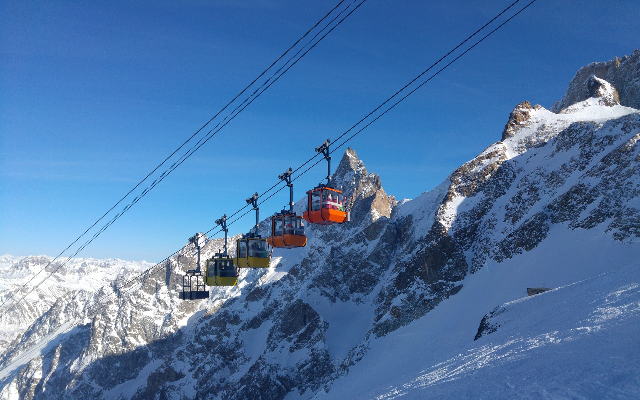
\includegraphics[width=\textwidth]{mountain}
        \caption{}
        \label{fig:parrots}
    \end{subfigure} 
    %~ %add desired spacing between images, e. g. ~, \quad, \qquad, \hfill etc. 
      %(or a blank line to force the subfigure onto a new line)    
    \begin{subfigure}[b]{0.24\textwidth}
        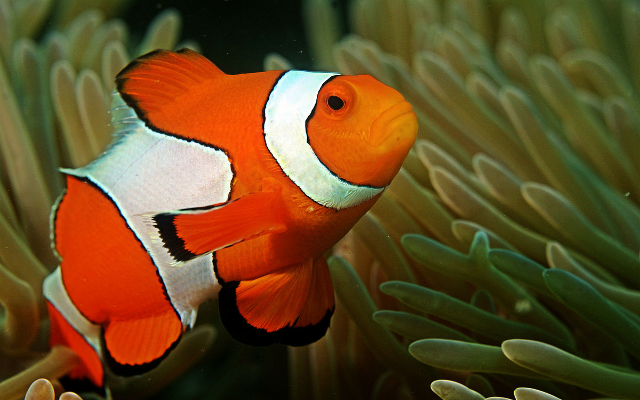
\includegraphics[width=\textwidth]{clownfish}
        \caption{}
        \label{fig:clownfish}
    \end{subfigure}
    %~ %add desired spacing between images, e. g. ~, \quad, \qquad, \hfill etc. 
      %(or a blank line to force the subfigure onto a new line)
    \begin{subfigure}[b]{0.24\textwidth}
        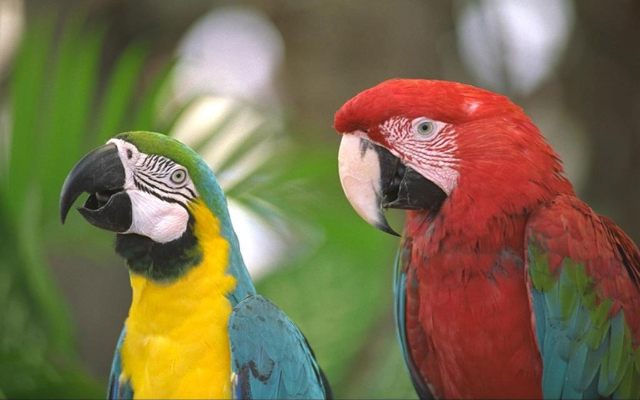
\includegraphics[width=\textwidth]{araras}
        \caption{}
        \label{fig:mountains}
    \end{subfigure}
                  
    \caption{Some examples of color images: One synthetic image {\small \textsf{\textbf{(a)}}} and three natural images [{\small \textsf{\textbf{(b) (c) (d)}}}].}\label{fig:color_images}    
\end{figure}


\section{Color}

Color is a physical property linked to the electromagnetic spectrum of light \citep{Beyerer.Leon.ea:Book:2016}. The perception of color in humans results from the quantity and wavelength captured by the eyes. This perception depends on many factors such as the type of surfaces or objects where the light is reflected, the environment and even the eyes of the observer. The perception of color is then an entirely arbitrary creation of our nervous system, and there is no way it is contained in the wavelengths or in light-reflecting objects and materials \citep{Goldstein:Book:2009} \citep{Beyerer.Leon.ea:Book:2016}. When an incident spectrum contains all frequencies in the range of visible wavelengths, humans perceive objects that reflect all frequencies as clear or \textit{white}. In the opposite case, when the material absorbs and does not reflect the visible frequencies, it is perceived as dark or \textit{black} {Gonzalez.Woods:Book:2008}. 

Although color has measurable physical properties, the interpretation and perception of this information is completely subjective. A clear example of this is the naming of colors. Some works in this regard state that the naming of colors varies according to culture and language \citep{Berlin.Kay:Book:1991}. However, it is possible to find a correlation between languages and identify eleven basic color terms in English language that  seem to be anchored across the different languages as points in a certain color space \citep{Kay.Regier:PNAS:2003}. The definition of a coherent color space to the final task is therefore essential to represent the color information digitally.


\section{Color representation}

The representation of color has evolved over time developing theories, such as the trichromatic theory or the opponent-colors theory \citep{Fairchild:Book:2005}, that attempt to explain the function of color vision. The result of these theories has been the development of abstract mathematical models that serve to represent colors as vectors or tuples of numbers. These vectors, which are mostly in three dimensions, can be arranged in a variety of ways. Such particular organizations are known as color models.

One of the main contributors in the creation of color spaces is the \textit{Commission Internationale de l'Éclairage} (CIE) \citep{CIE:Journal:1932}, who defined the three standard primaries of color $X$, $Y$ and $Z$. These primaries allow to define any visible color of the spectrum (see figure \ref{fig:visual_spectrum}) as a weighted sum of the three primary colors. They are defined mathematically with positive color-matching functions that specify the amount of each primary needed to describe any spectral color \citep{Wright:BookCh2:2007}. This color model is known as the CIE 1931 XYZ.

The \textbf{XYZ color model} quantify an object’s color using a standardized method taking into account the human eye’s (observer) response to these colors in the calculation. $X$, $Y$ and $Z$ are the amount of each primary needed to produce a desired color
\begin{eqnarray} 
 C(\lambda) = (X,Y,Z) \label{eq:XYZ_color}
\end{eqnarray}
where the primary $Y$ is chosen such that its colour-matching function exactly matches the luminous-efficiency function for the human eye, i.e., $Y$ measure the luminance of a color \citep{Wright:BookCh2:2007}. Therefore, to define a color in this space, we need to provide the weights fot the $X$, $Y$ and $Z$ primaries, for example, color $=xX + yY + zZ$, where 
\begin{eqnarray} 
	x = \frac{X}{X+Y+Z} \\
	y = \frac{Y}{X+Y+Z} \\ 
	z = \frac{Z}{X+Y+Z} = 1-x-y \label{eq:xyz_color_coords}
\end{eqnarray}

Under this representation, we can ignore the dimension of the luminance by the normalizacion of the primaries with the total light intensity; $x+y+z=1$. This allow to show all visibles colors of the spectrum in the chromaticity diagram (see figure \ref{fig:chrom_diagram}). The $x$ and $y$ axis give the normalised amounts of the $X$ and $Y$ primaries for a particular colour, and hence $z = 1 - x - y$ gives the amount of the $Z$ primary required. Chromaticity depends on dominant wavelength and saturation, and is independent of luminous energy. Colours with the same chromaticity but different luminance, all map to the same point within this region.

\begin{figure}[!ht]
    \centering
    \begin{subfigure}[b]{0.45\textwidth}
        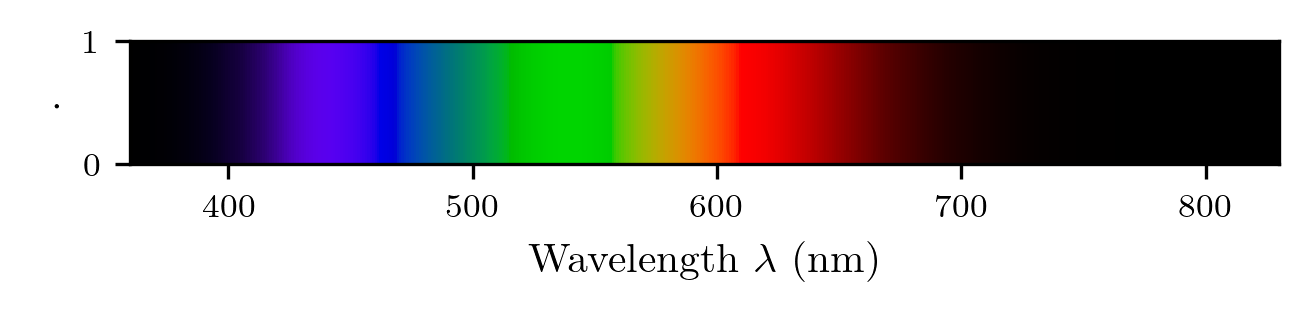
\includegraphics[width=\textwidth]{CIE_visible_spectrum}
        \caption{}
        \label{fig:visual_spectrum}
    \end{subfigure}
    %~ %add desired spacing between images, e. g. ~, \quad, \qquad, \hfill etc. 
      %(or a blank line to force the subfigure onto a new line)
    \begin{subfigure}[b]{0.45\textwidth}
        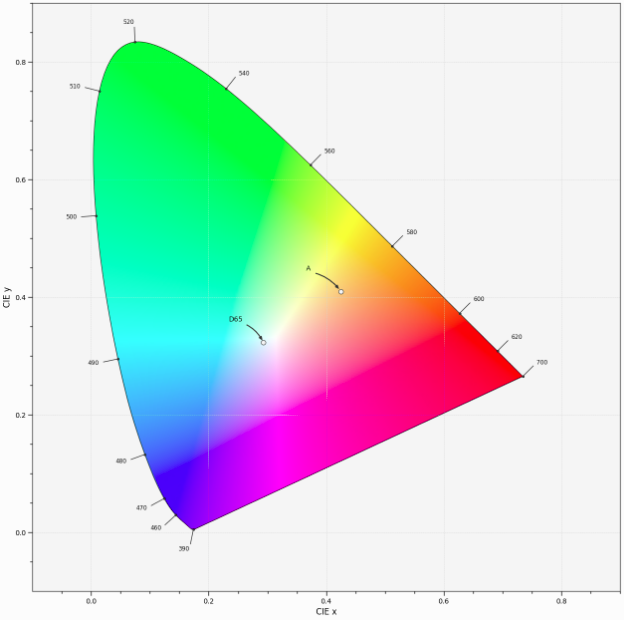
\includegraphics[width=\textwidth]{CIE_chromaticity_diagram}
        \caption{}
        \label{fig:chrom_diagram}
    \end{subfigure} 
                      
    \caption{CIE 1931 2 Degree Standard Observer: visible light spectrum {\small \textsf{\textbf{(a)}}} and chromaticity diagram {\small \textsf{\textbf{(b)}}}.}\label{fig:cie_standard_observer}    
\end{figure}


The \textbf{RGB color model} is an additive model coming from the three-component theory. This model consists of three independent planes, represented as a three
dimensional vector, one in each of the primary colours: red, green and blue. Therefore, to define a color in this model, we specify the proportion of red, green, and blue colors. 

\textbf{HSV color model}

\textbf{HSL color model}

\textbf{LAB color model} (also known as CIEL*a*b* or CIELAB)


\begin{itemize}

	\item \textbf{RBG (Red-Green-Blue)} A color space that maps the amount of red, green and blue light perceived to reproduce the visible color gamut.
	\item \textbf{HSV (Hue-Saturation-Value) and HSL (Hue-Saturation-Lightness)} Alternative representations to the RGB color space that more closely aligns with the way human vision perceives color-creating attributes.
	\item \textbf{Lab (CIEL*a*b*) / Luv (CIEL*u*v*).} A color space where L compenent represents luminance and a* and b* (resp. u* v*) components represent chroma. This representation was created to reflect the high sensitivity of humans to changes in luminance in the perception of color.
\end{itemize}


\begin{figure}[!ht]
    \begin{subfigure}[t]{\dimexpr0.3\textwidth+20pt\relax}
    	\makebox[20pt]{\raisebox{35pt}{ \rotatebox[origin=c]{90} {\small \textsf{\textbf{Input image}}} }}%
    	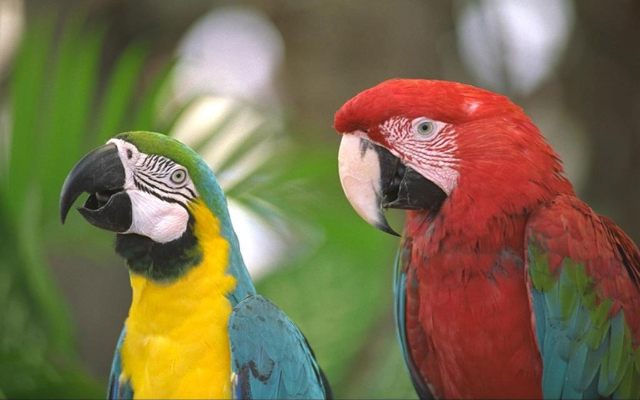
\includegraphics[width=\dimexpr\linewidth-20pt\relax]{araras}
    \end{subfigure} \\    
     
    \begin{subfigure}[t]{\dimexpr0.3\textwidth+20pt\relax}
    	\makebox[20pt]{\raisebox{35pt}{ \rotatebox[origin=c]{90} {\small \textsf{\textbf{RGB channels}}} }}%
    	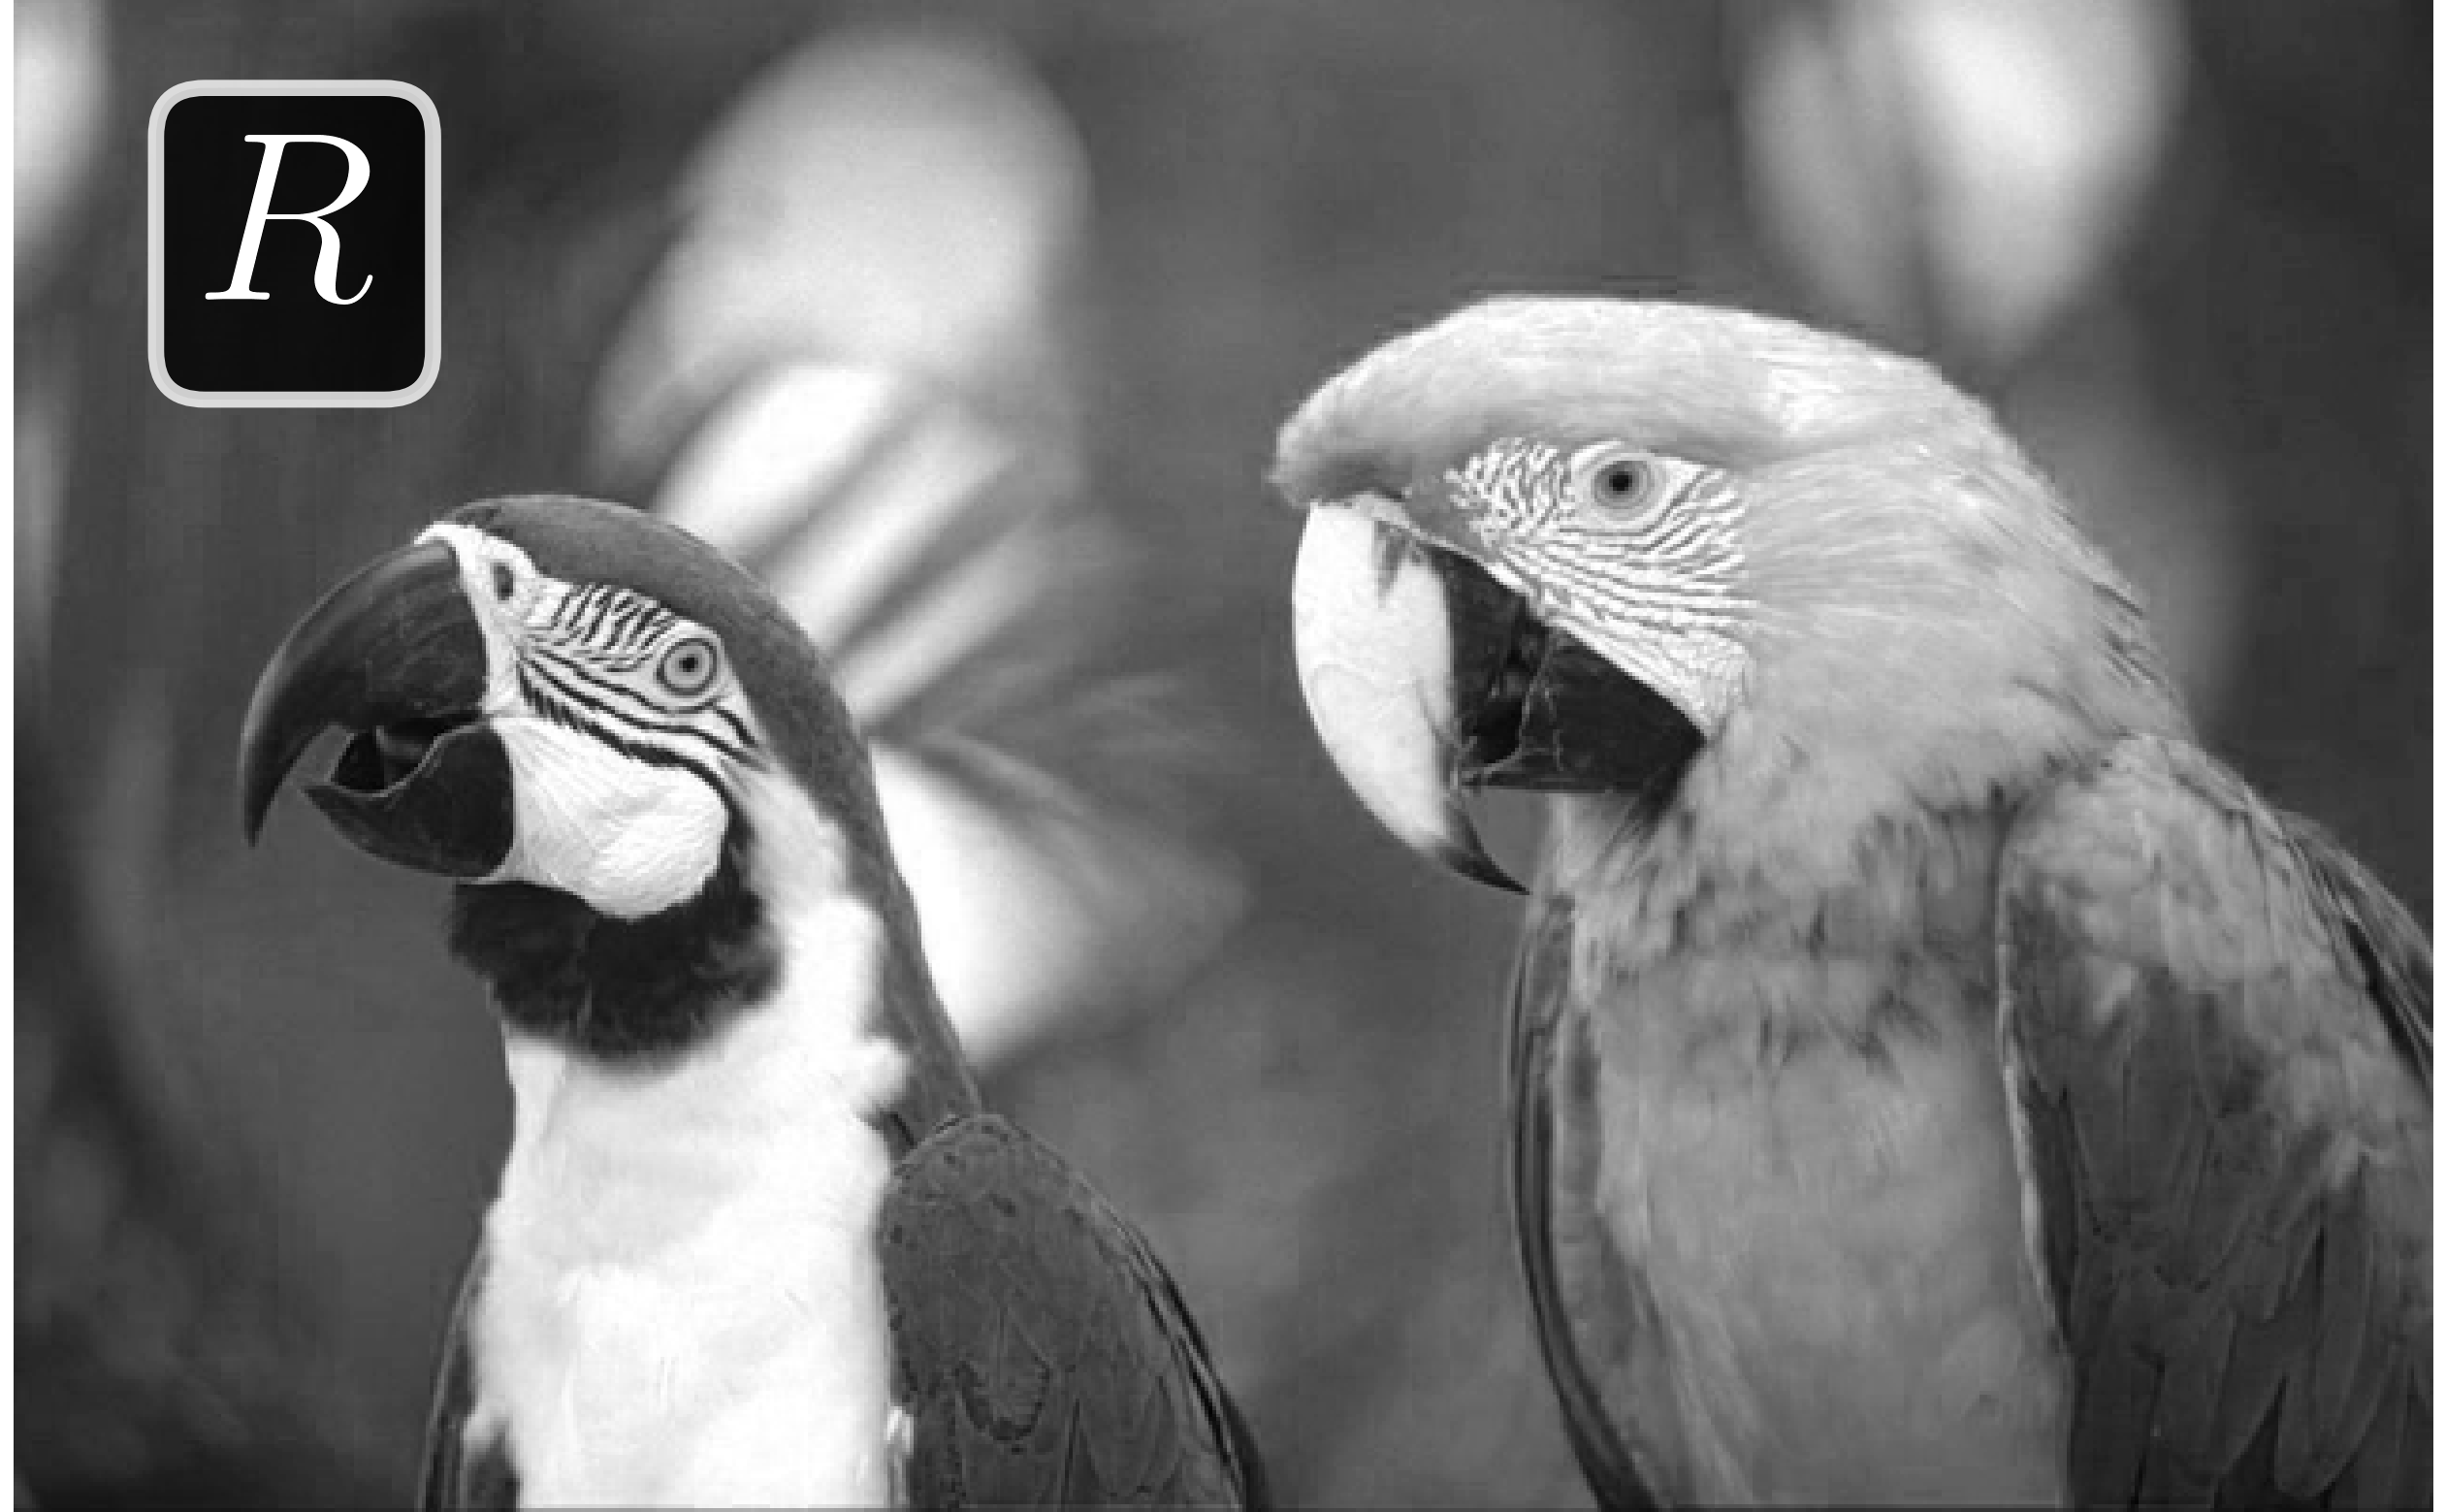
\includegraphics[width=\dimexpr\linewidth-20pt\relax]{araras_R}
    \end{subfigure}      
    ~ %add desired spacing between images, e. g. ~, \quad, \qquad, \hfill etc. 
      %(or a blank line to force the subfigure onto a new line)
    \begin{subfigure}[b]{0.3\textwidth}
        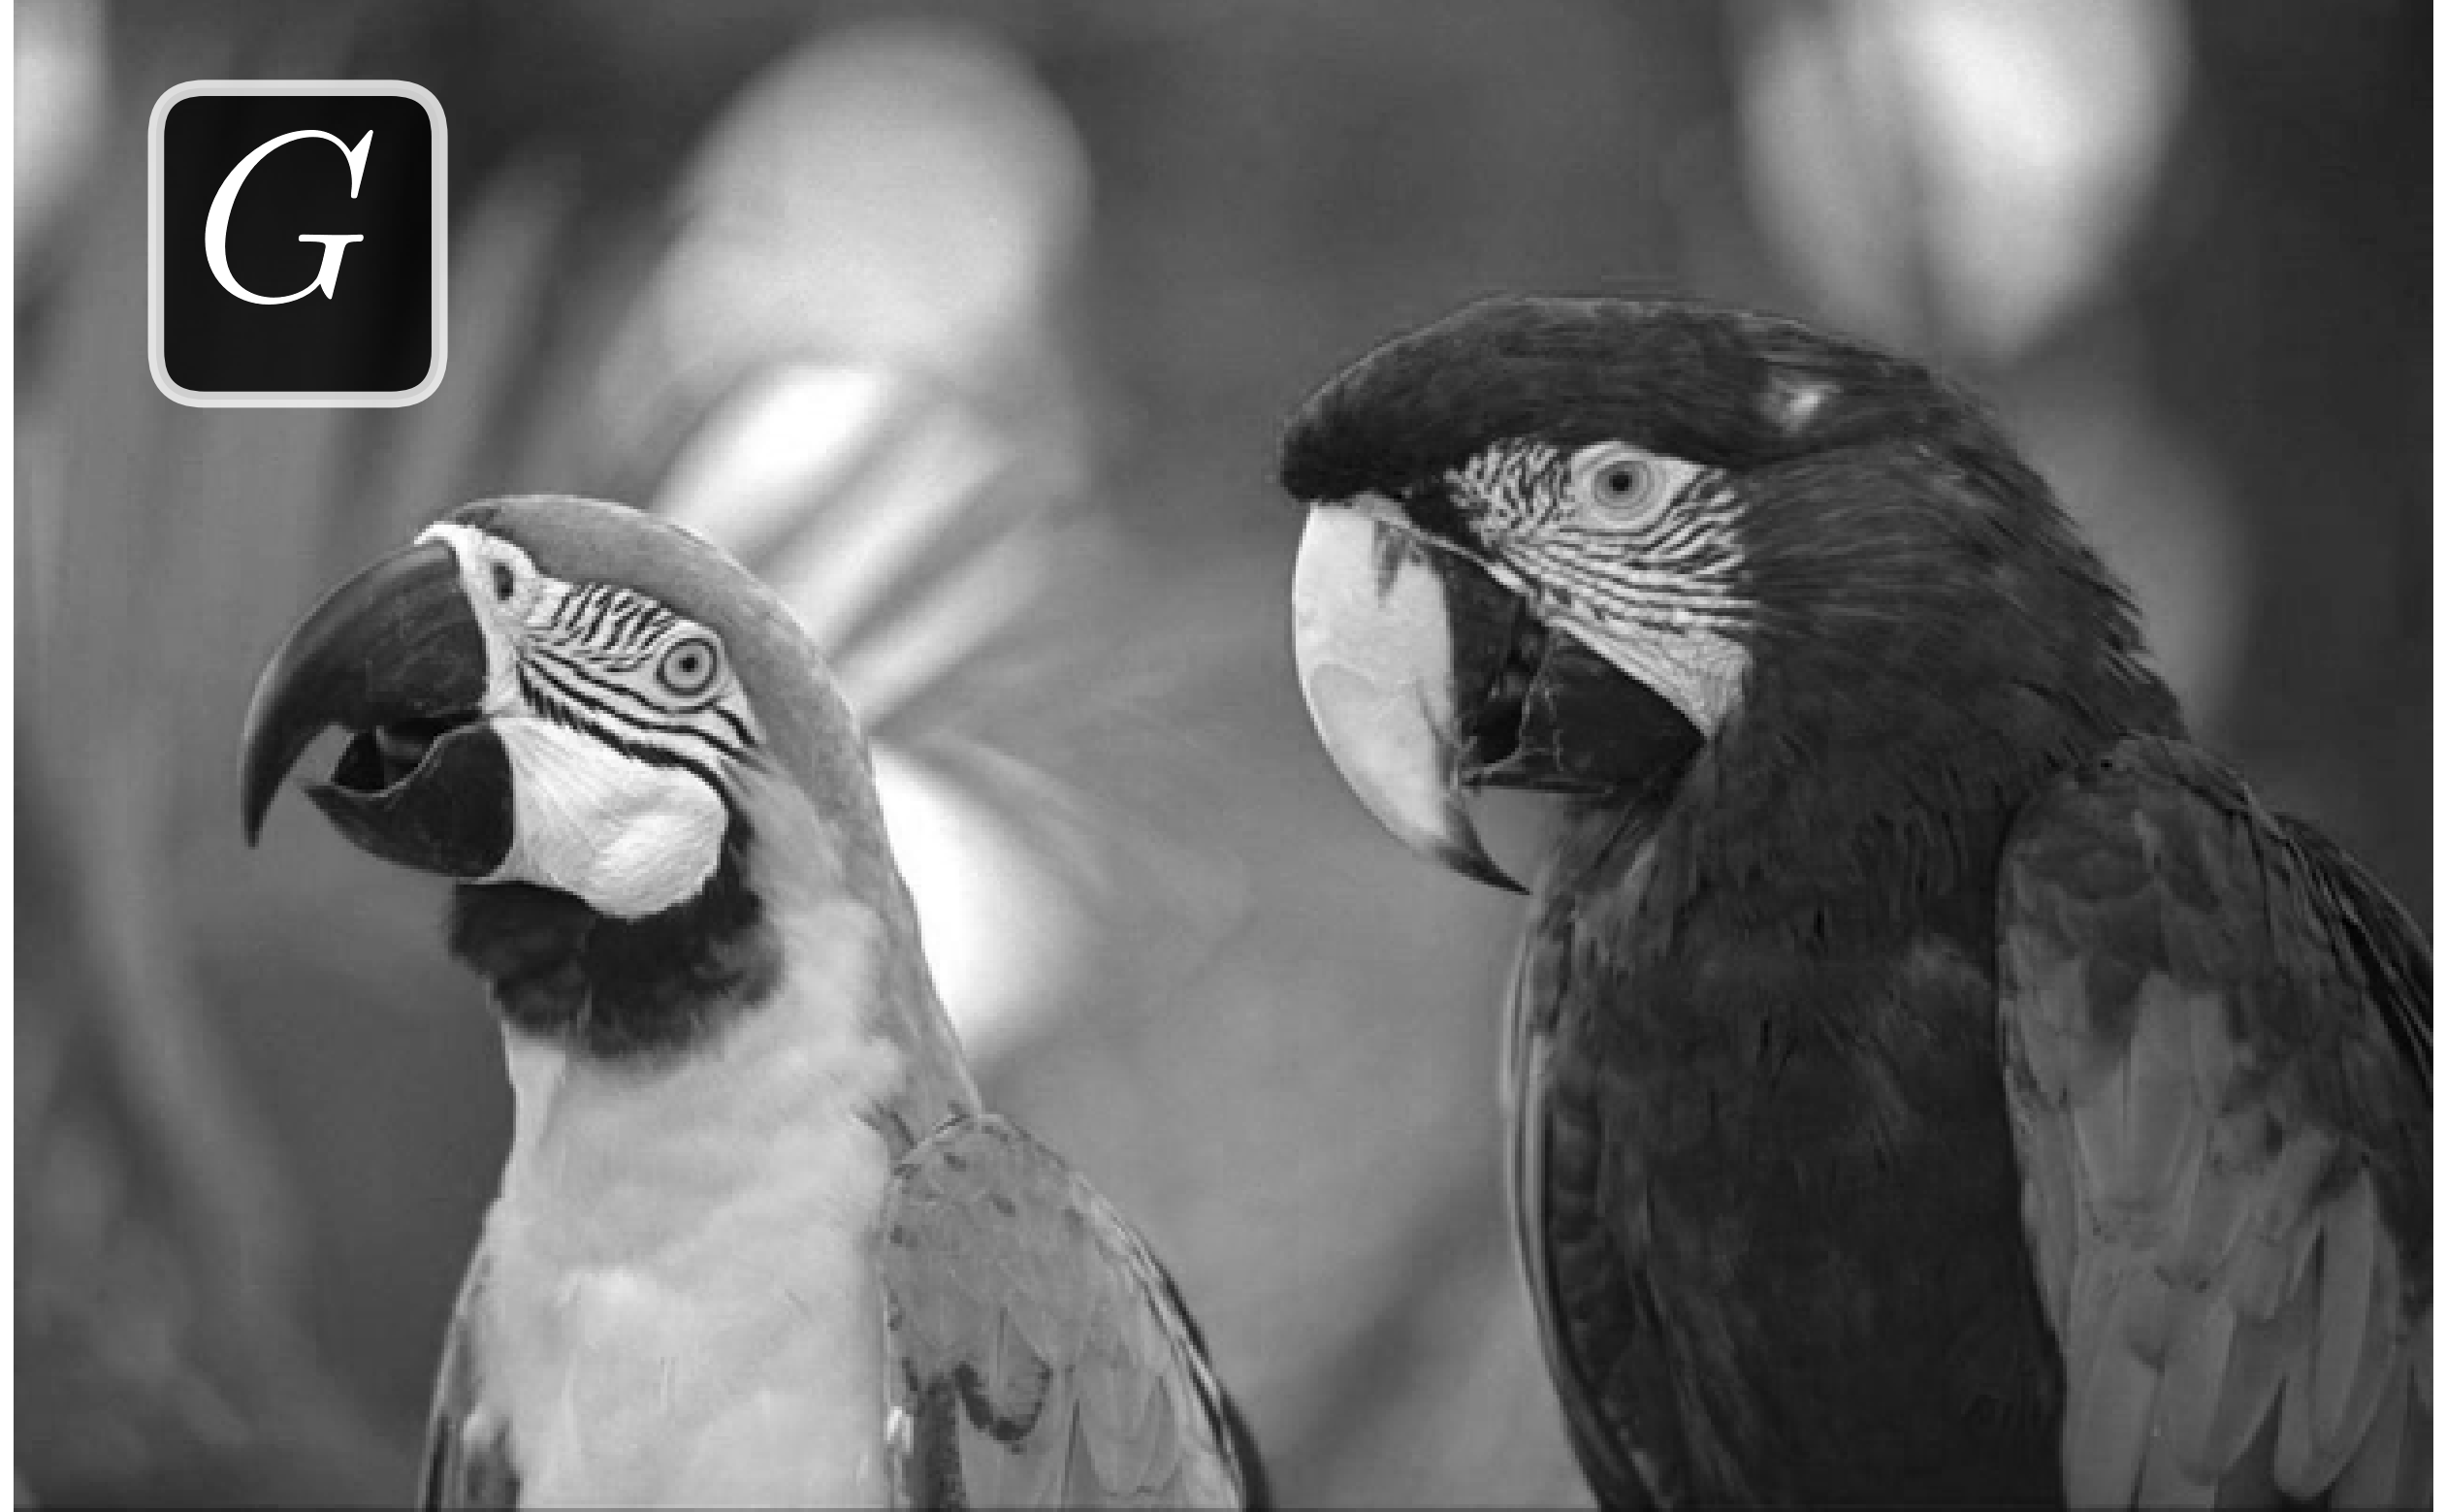
\includegraphics[width=\textwidth]{araras_G}
    \end{subfigure}
    ~ %add desired spacing between images, e. g. ~, \quad, \qquad, \hfill etc. 
      %(or a blank line to force the subfigure onto a new line)
    \begin{subfigure}[b]{0.3\textwidth}
        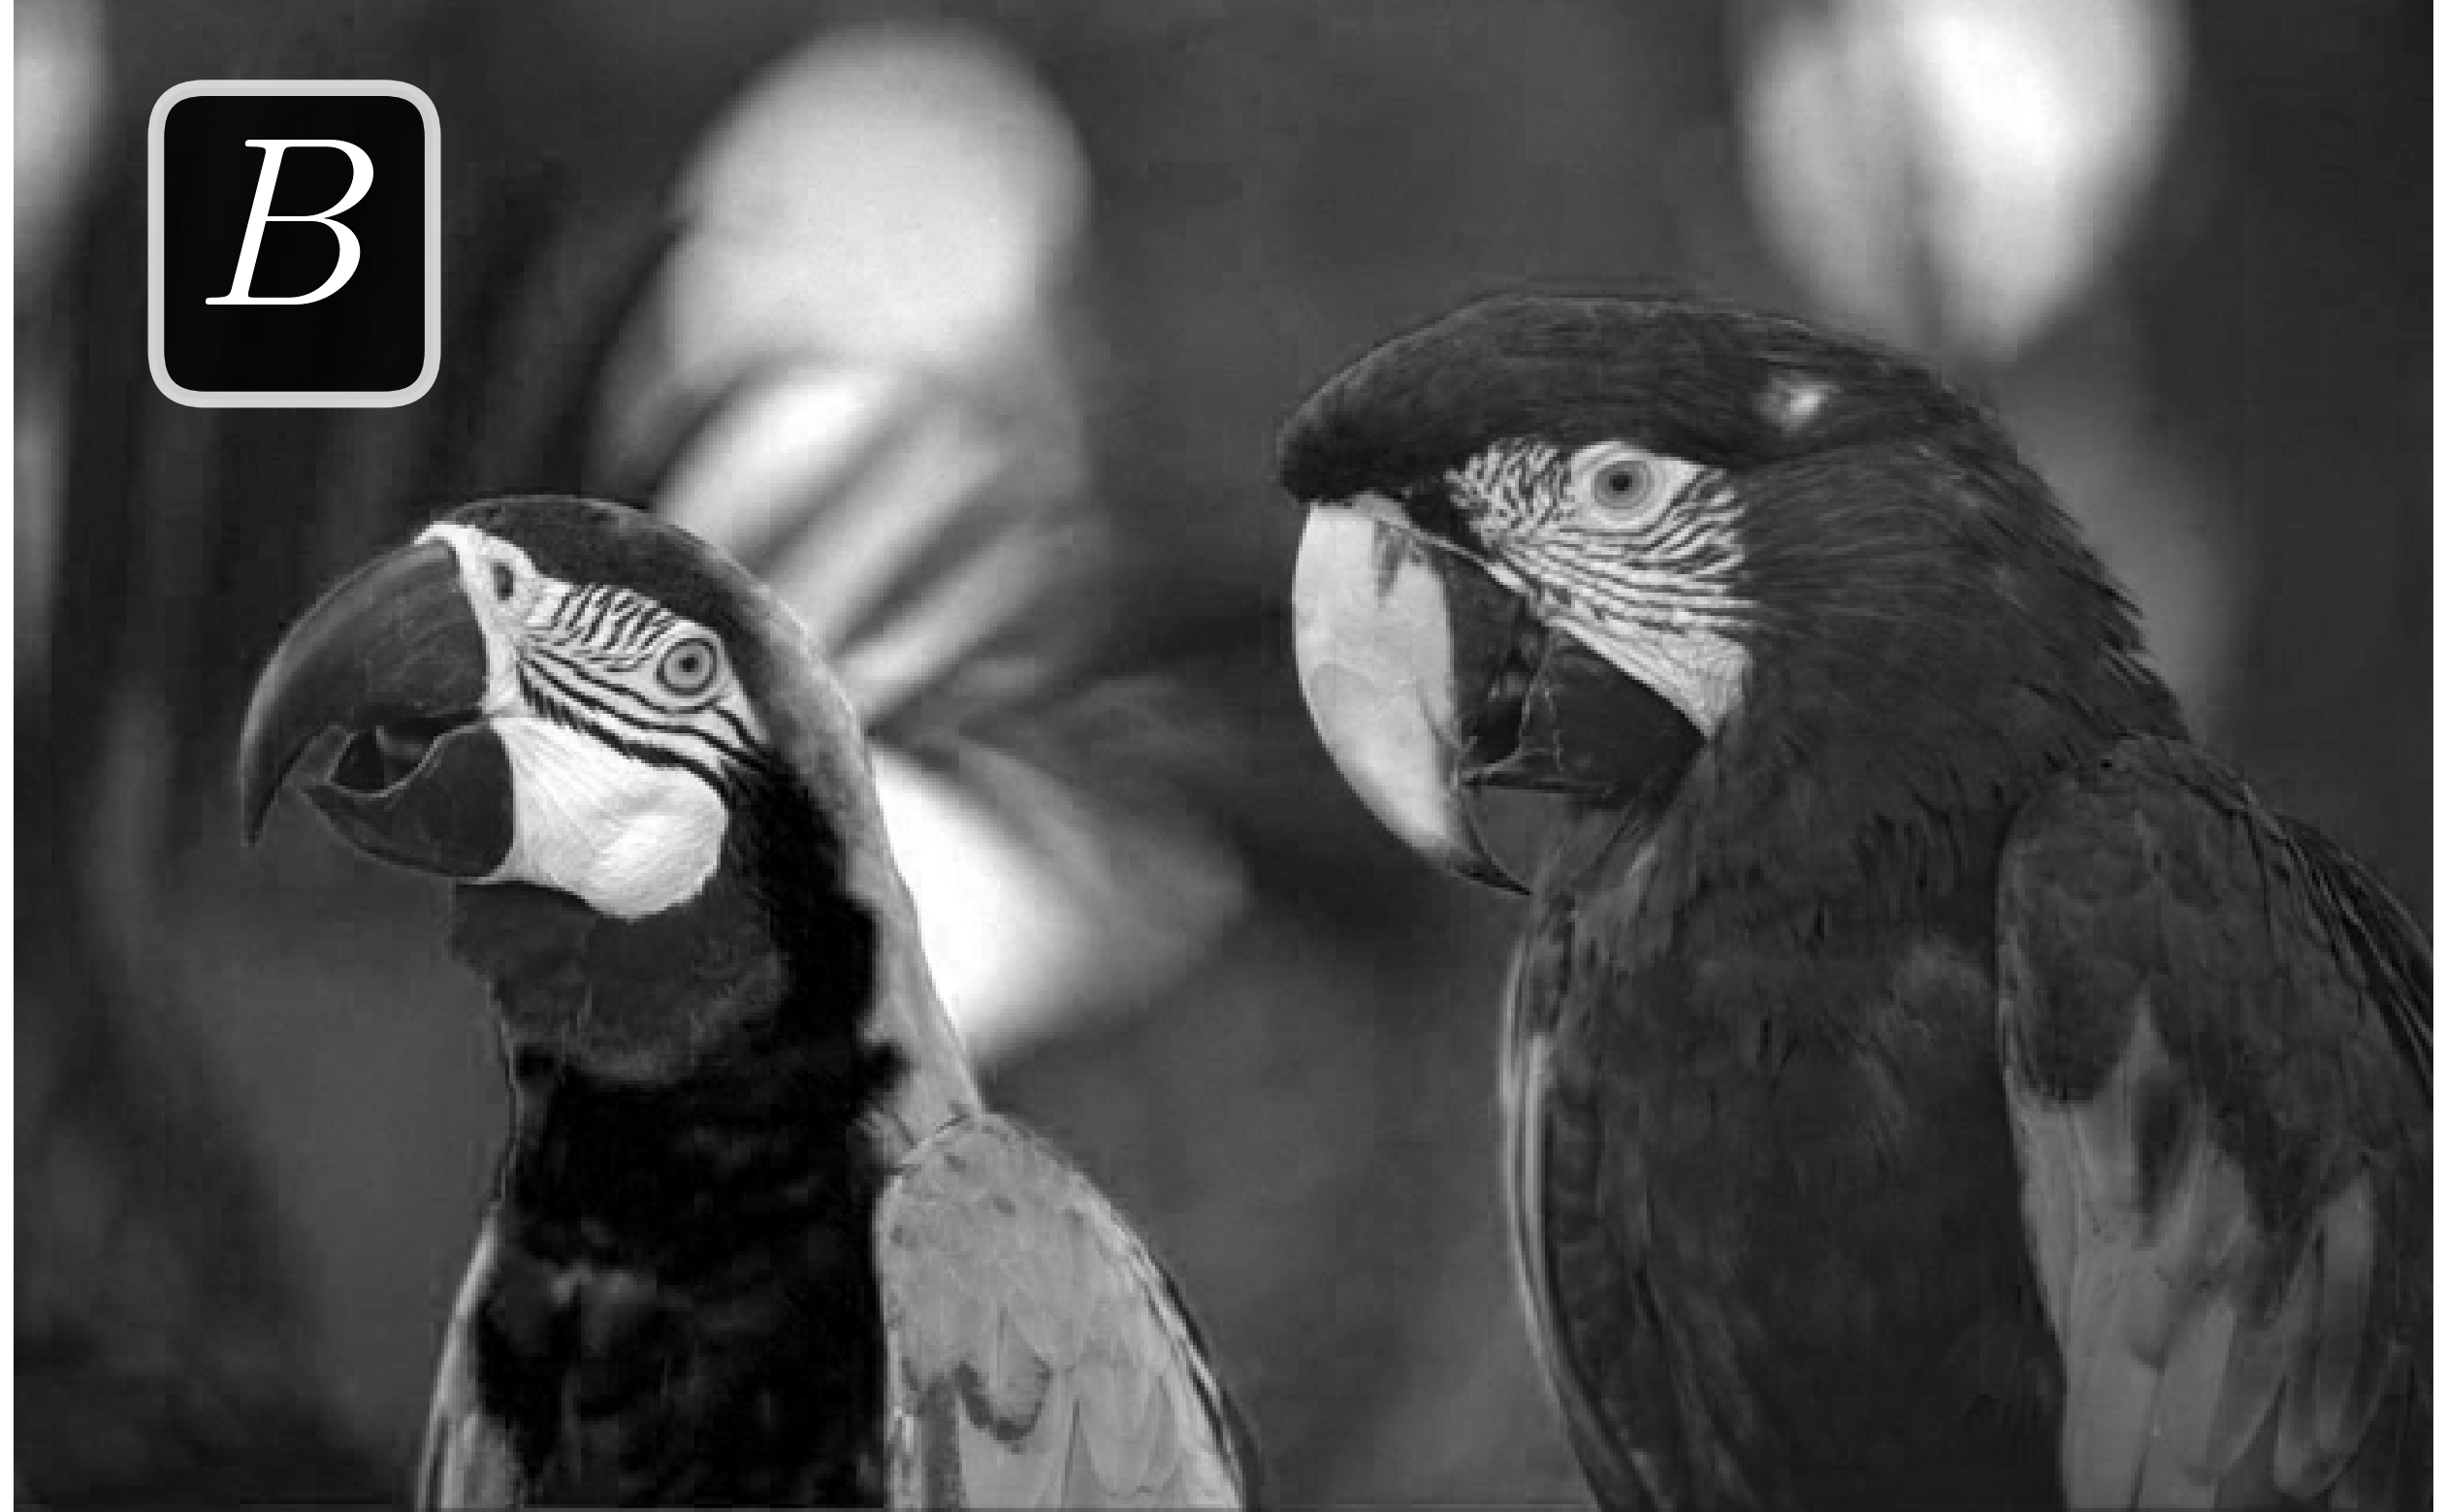
\includegraphics[width=\textwidth]{araras_B}
    \end{subfigure} \vspace{5pt}      
    
    \begin{subfigure}[t]{\dimexpr0.3\textwidth+20pt\relax}
    	\makebox[20pt]{\raisebox{35pt}{ \rotatebox[origin=c]{90} {\small \textsf{\textbf{HSV channels}}} }}%
    	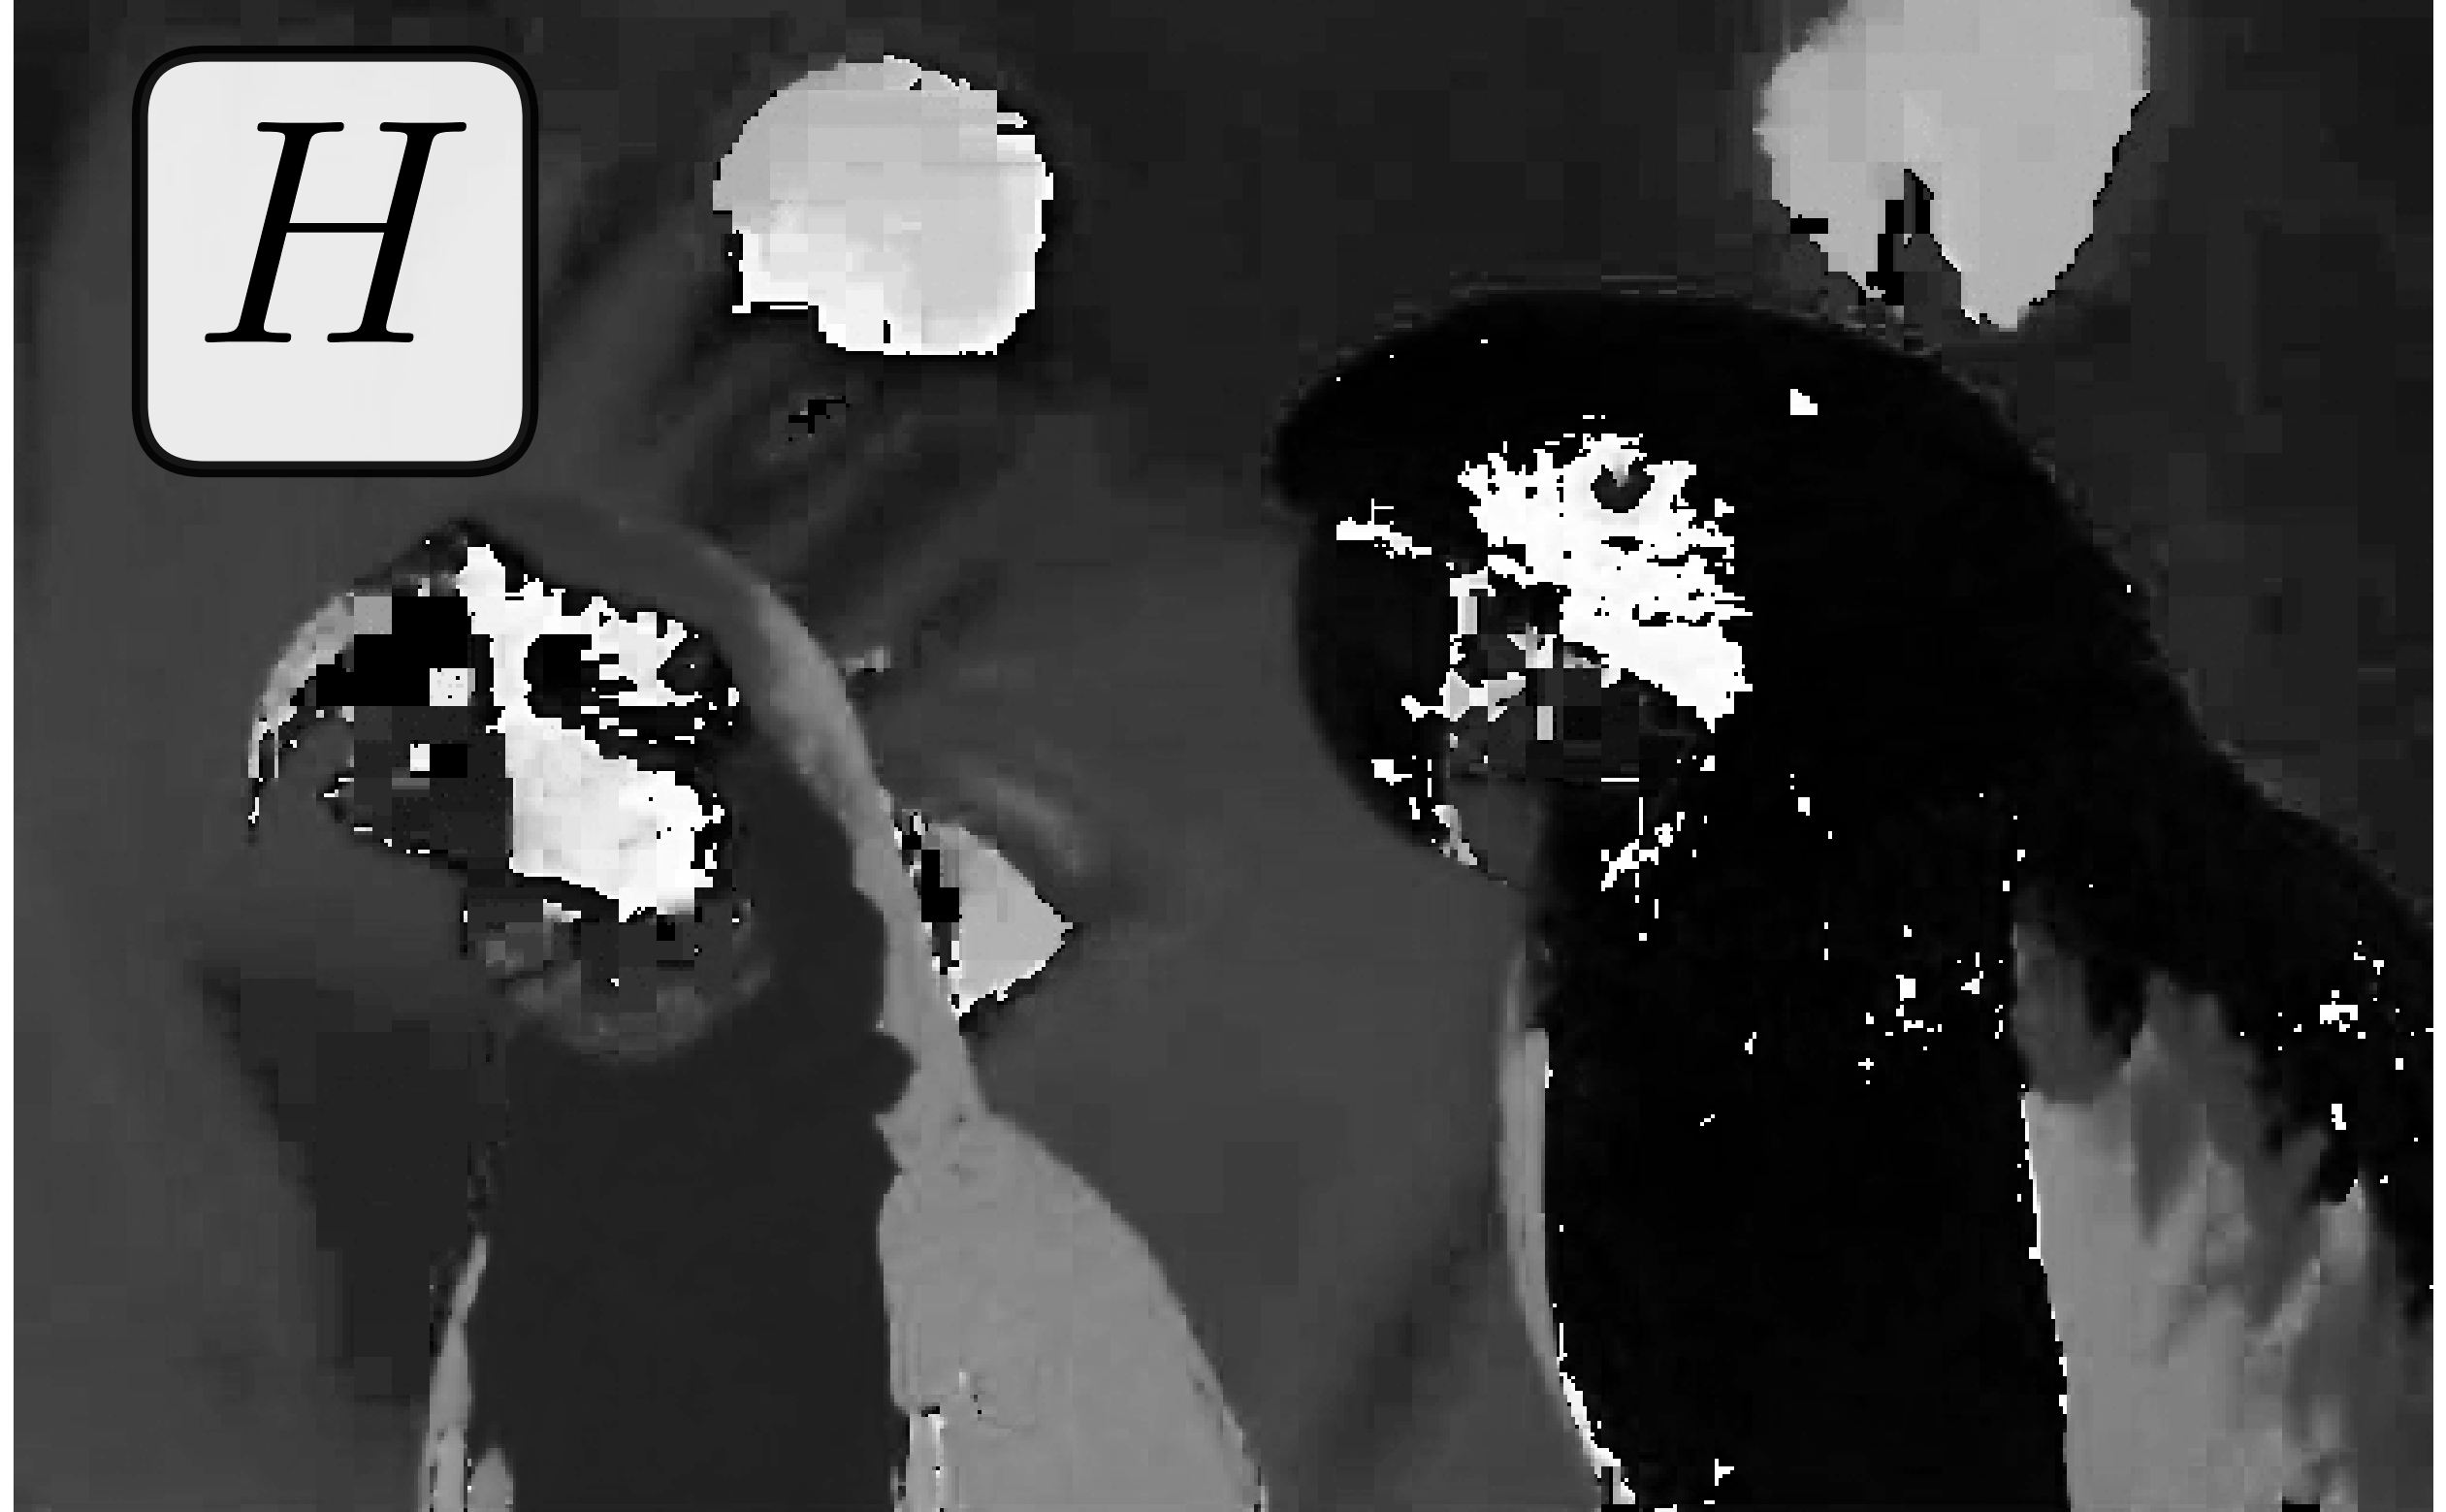
\includegraphics[width=\dimexpr\linewidth-20pt\relax]{araras_H}
    \end{subfigure}     
    ~ %add desired spacing between images, e. g. ~, \quad, \qquad, \hfill etc. 
      %(or a blank line to force the subfigure onto a new line)
    \begin{subfigure}[b]{0.3\textwidth}
        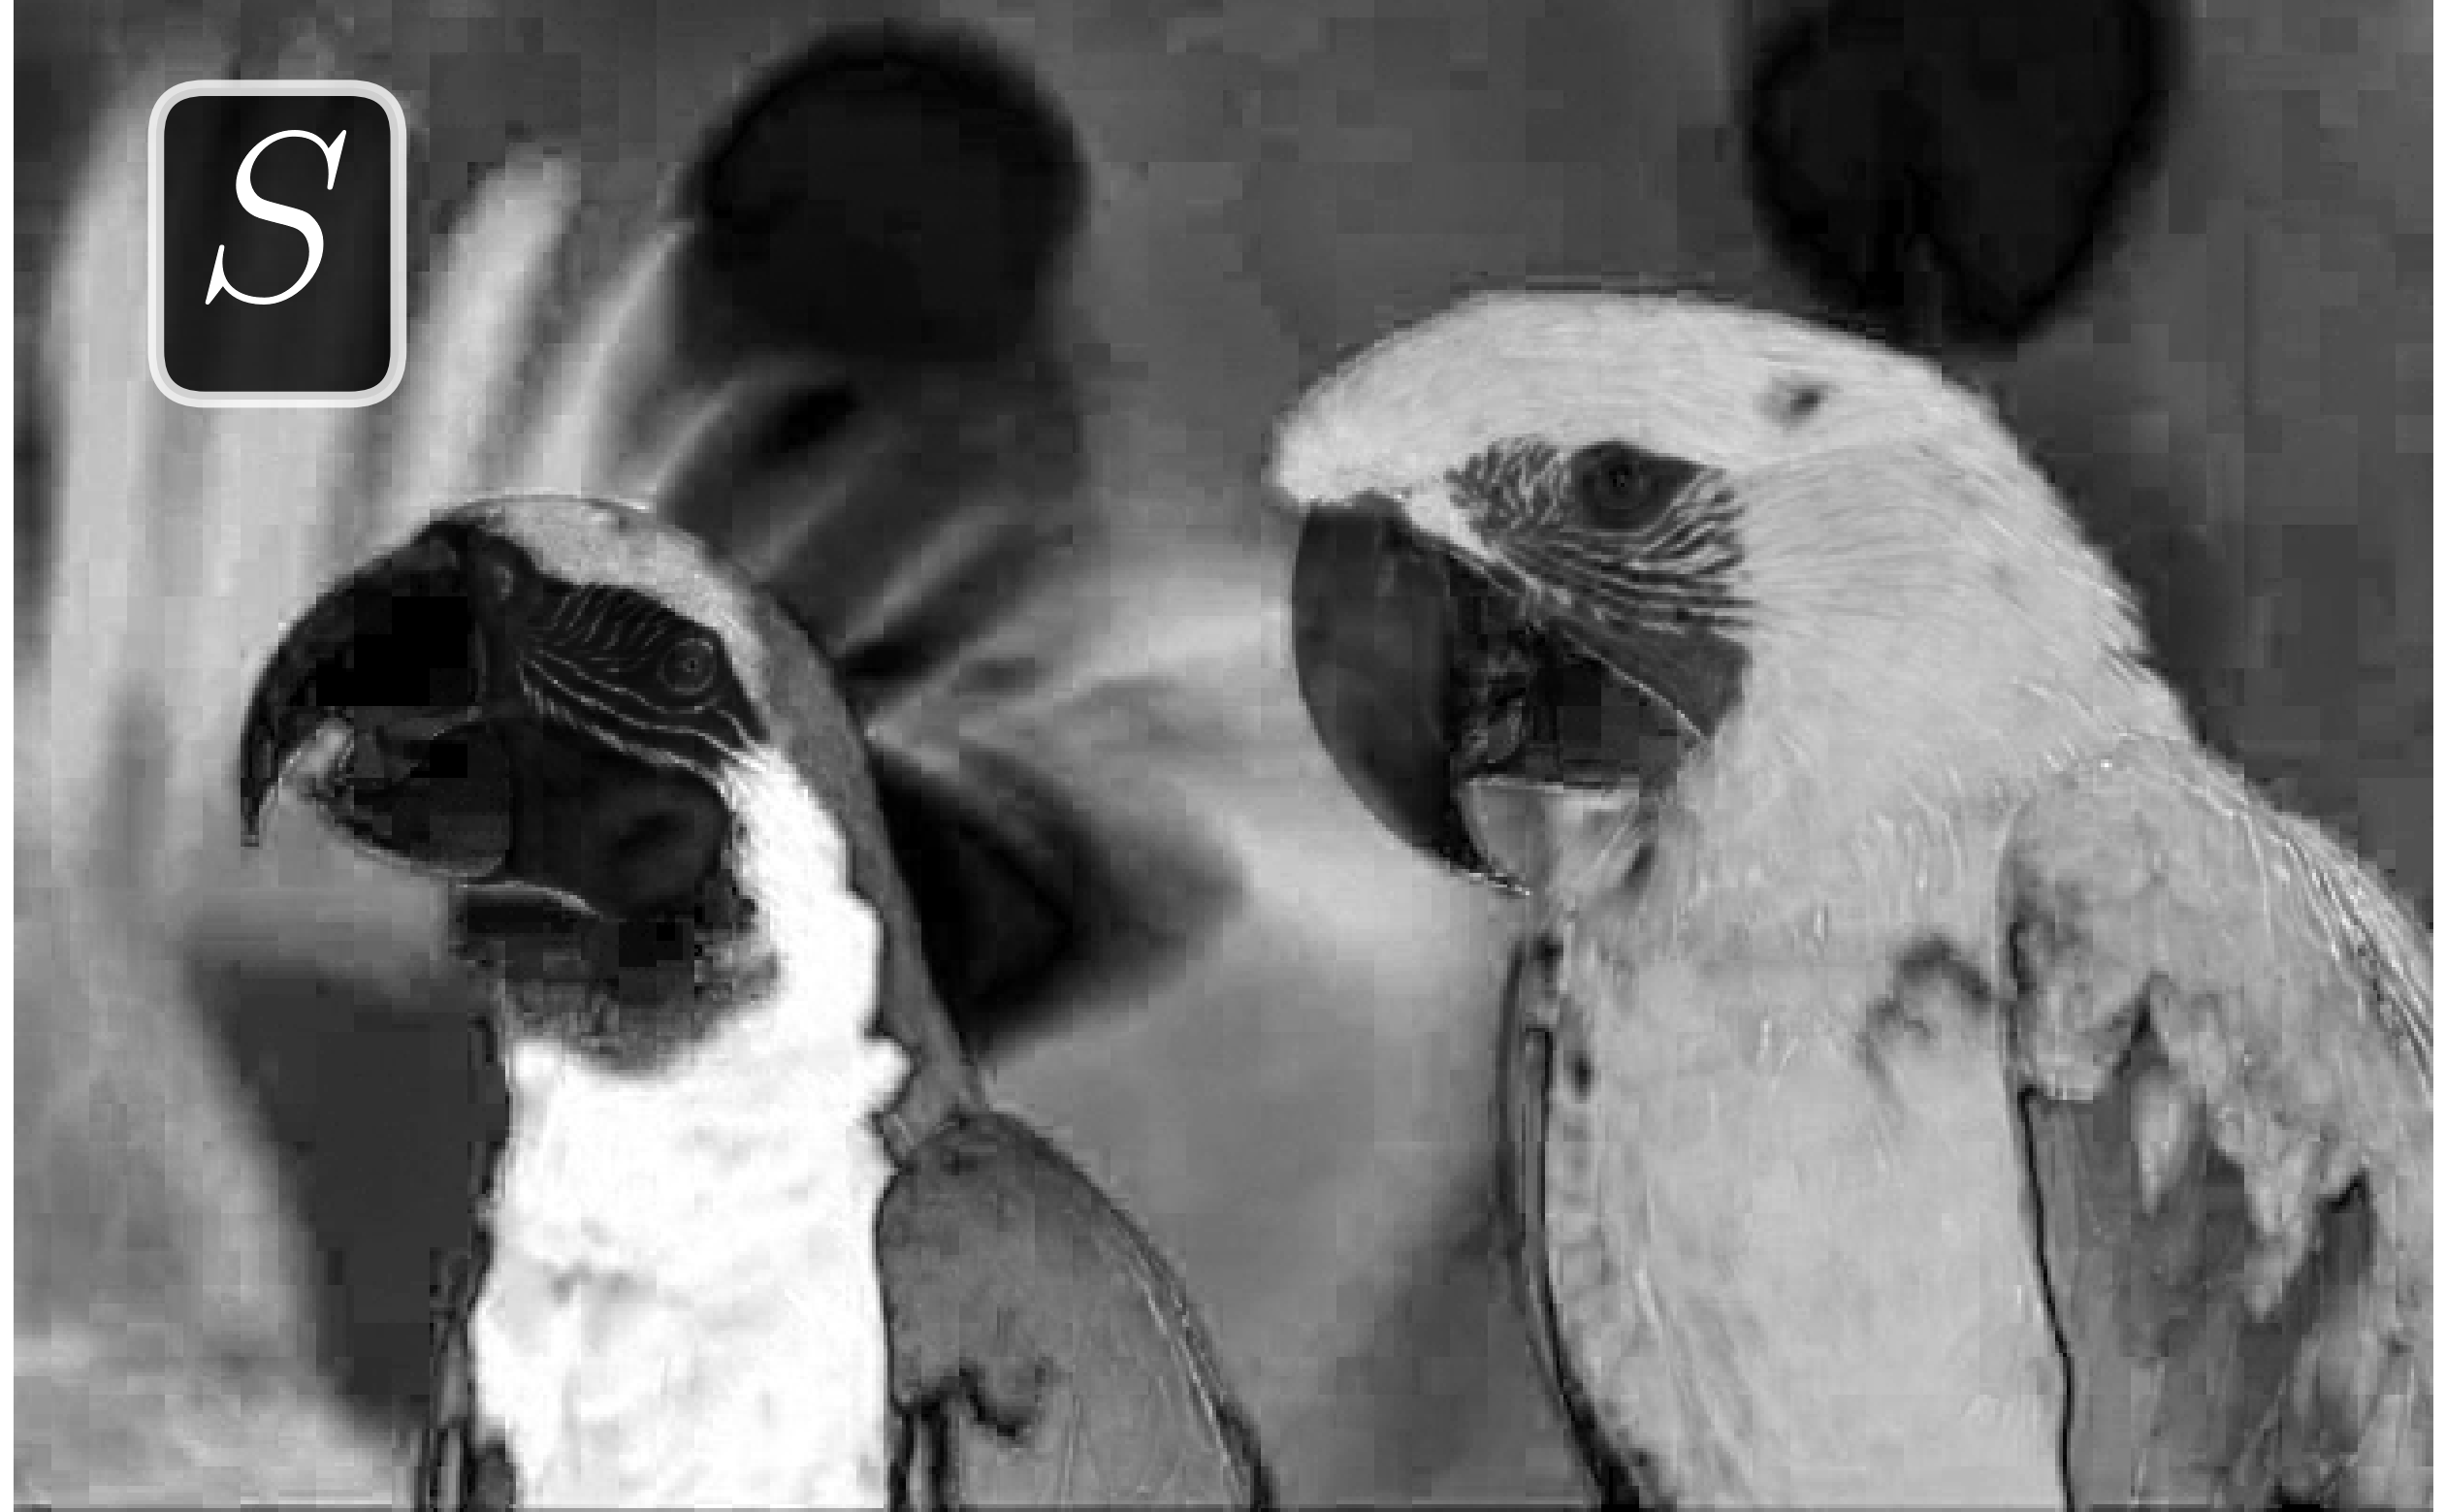
\includegraphics[width=\textwidth]{araras_S}
    \end{subfigure}
    ~ %add desired spacing between images, e. g. ~, \quad, \qquad, \hfill etc. 
      %(or a blank line to force the subfigure onto a new line)
    \begin{subfigure}[b]{0.3\textwidth}
        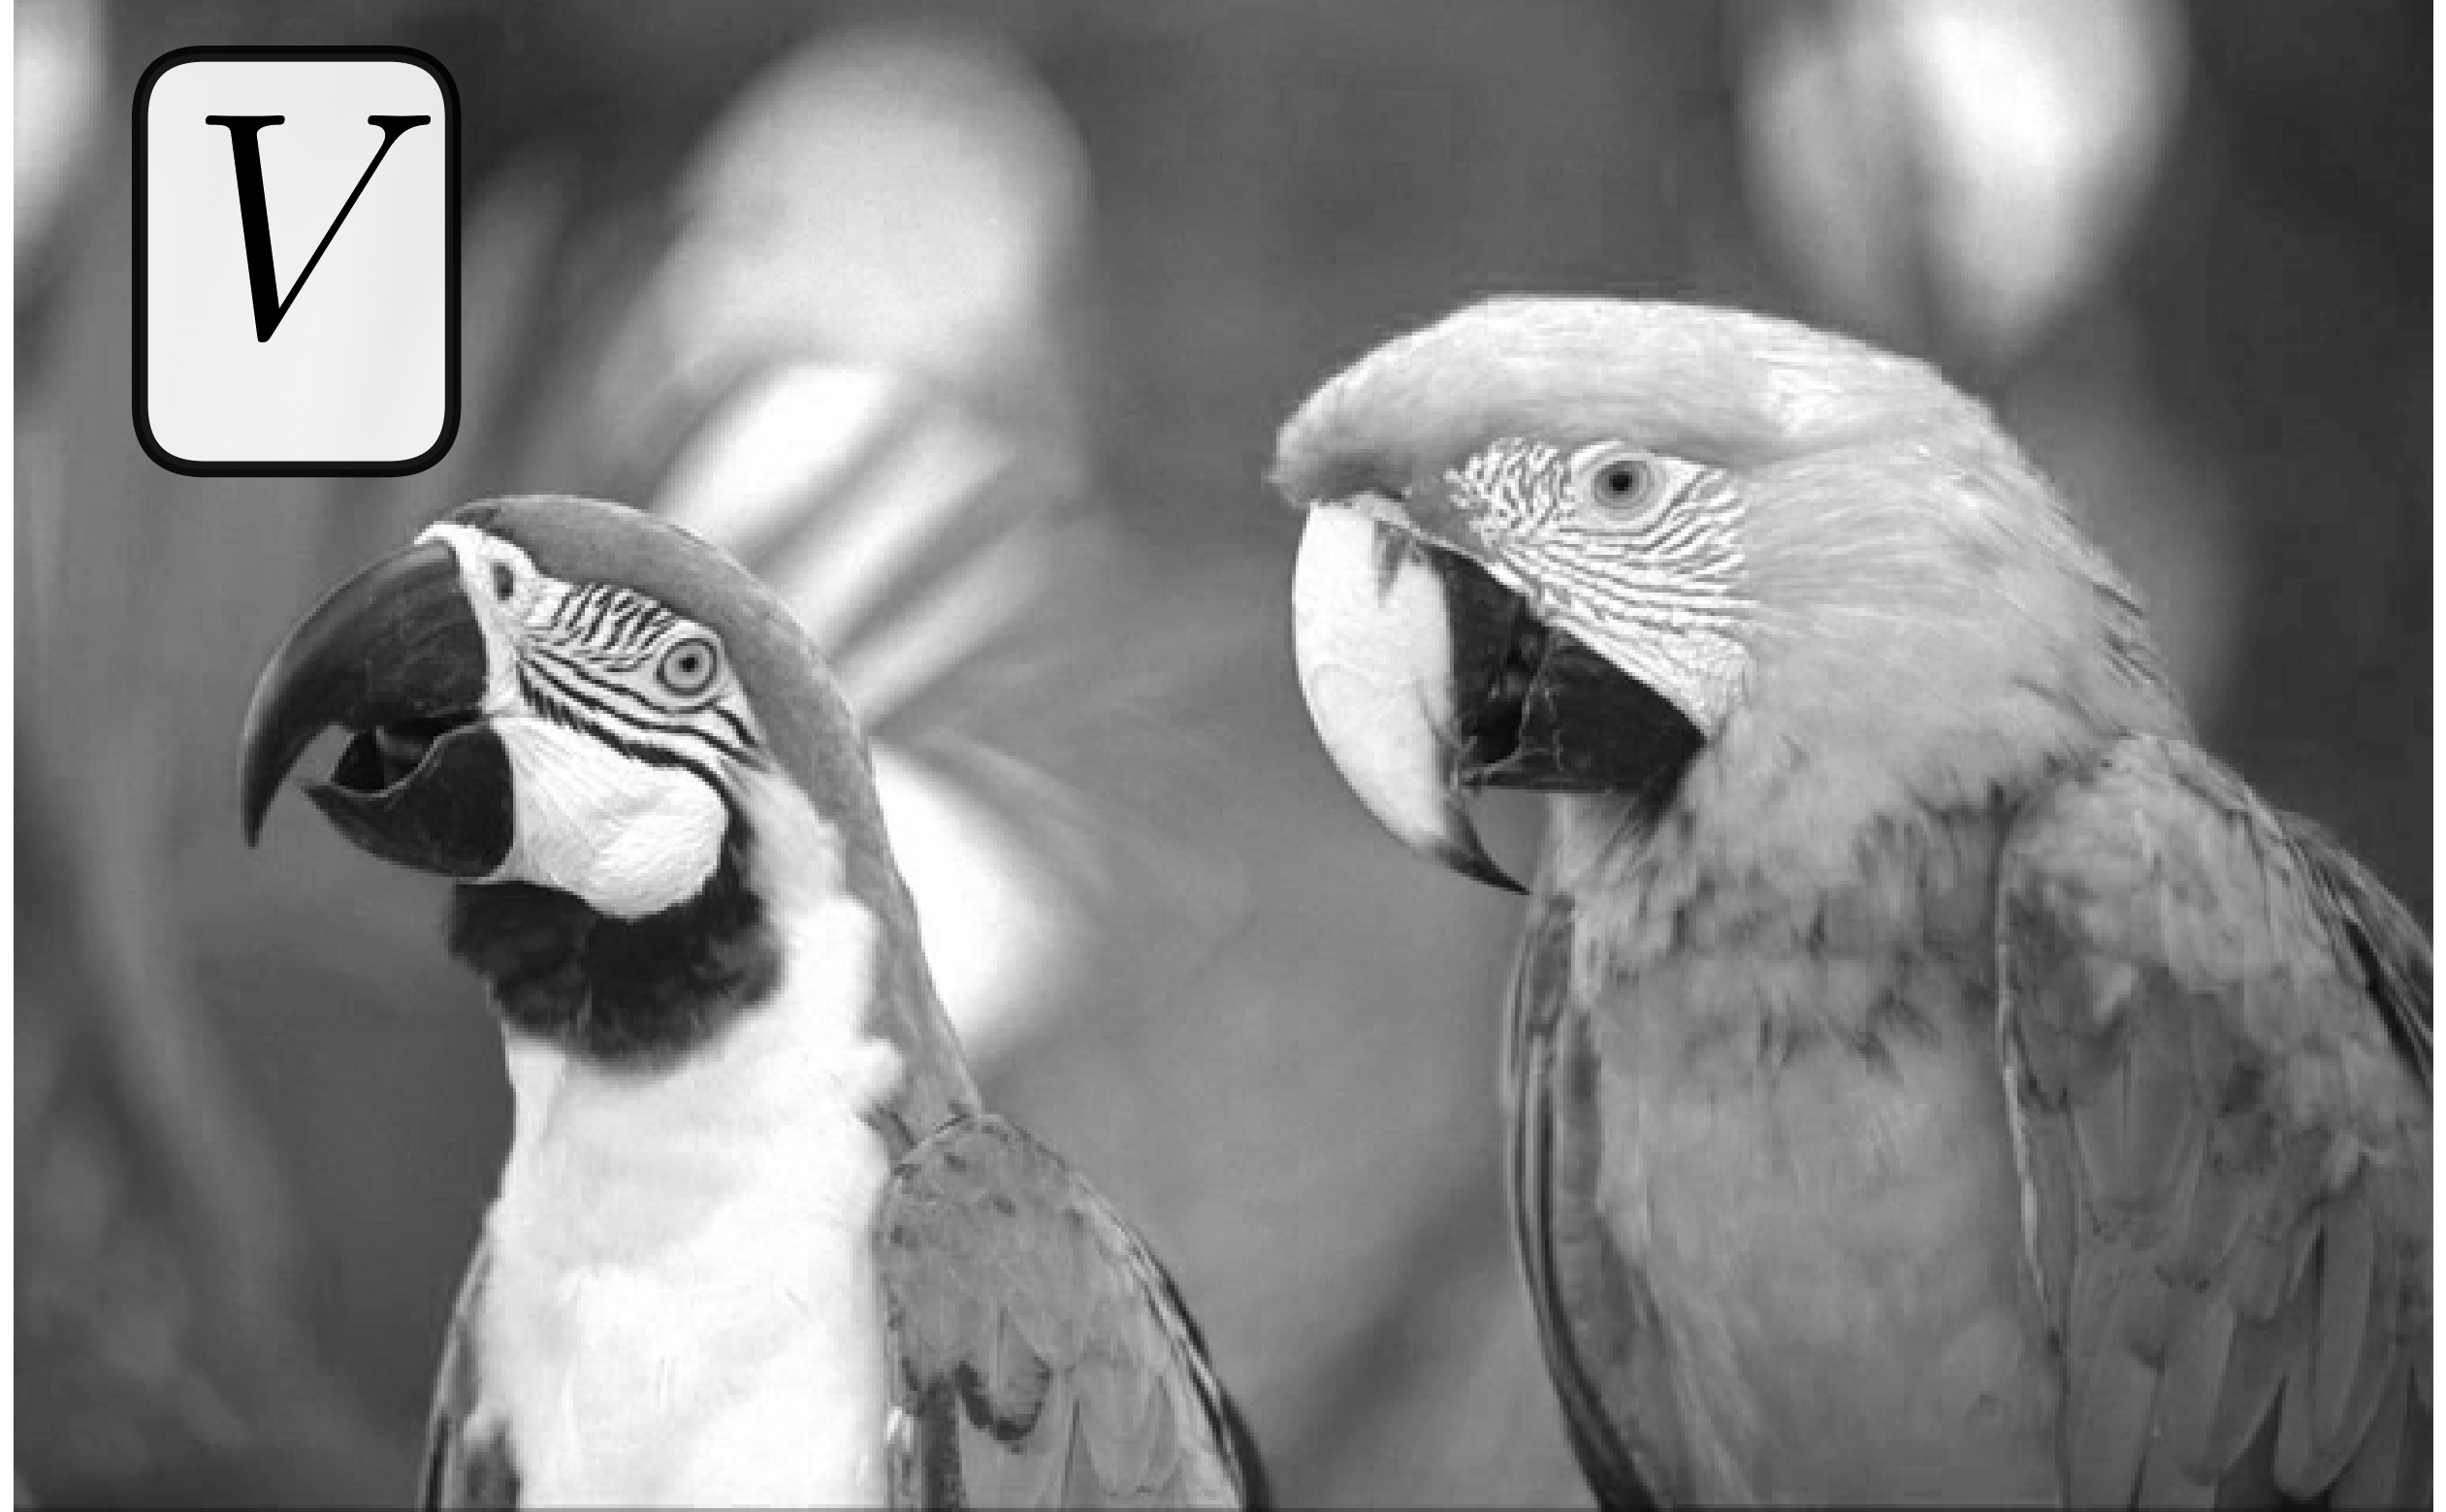
\includegraphics[width=\textwidth]{araras_V}
    \end{subfigure} \vspace{5pt}  
        
    \begin{subfigure}[t]{\dimexpr0.3\textwidth+20pt\relax}
    	\makebox[20pt]{\raisebox{35pt}{ \rotatebox[origin=c]{90} {\small \textsf{\textbf{LAB channels}}} }}%
    	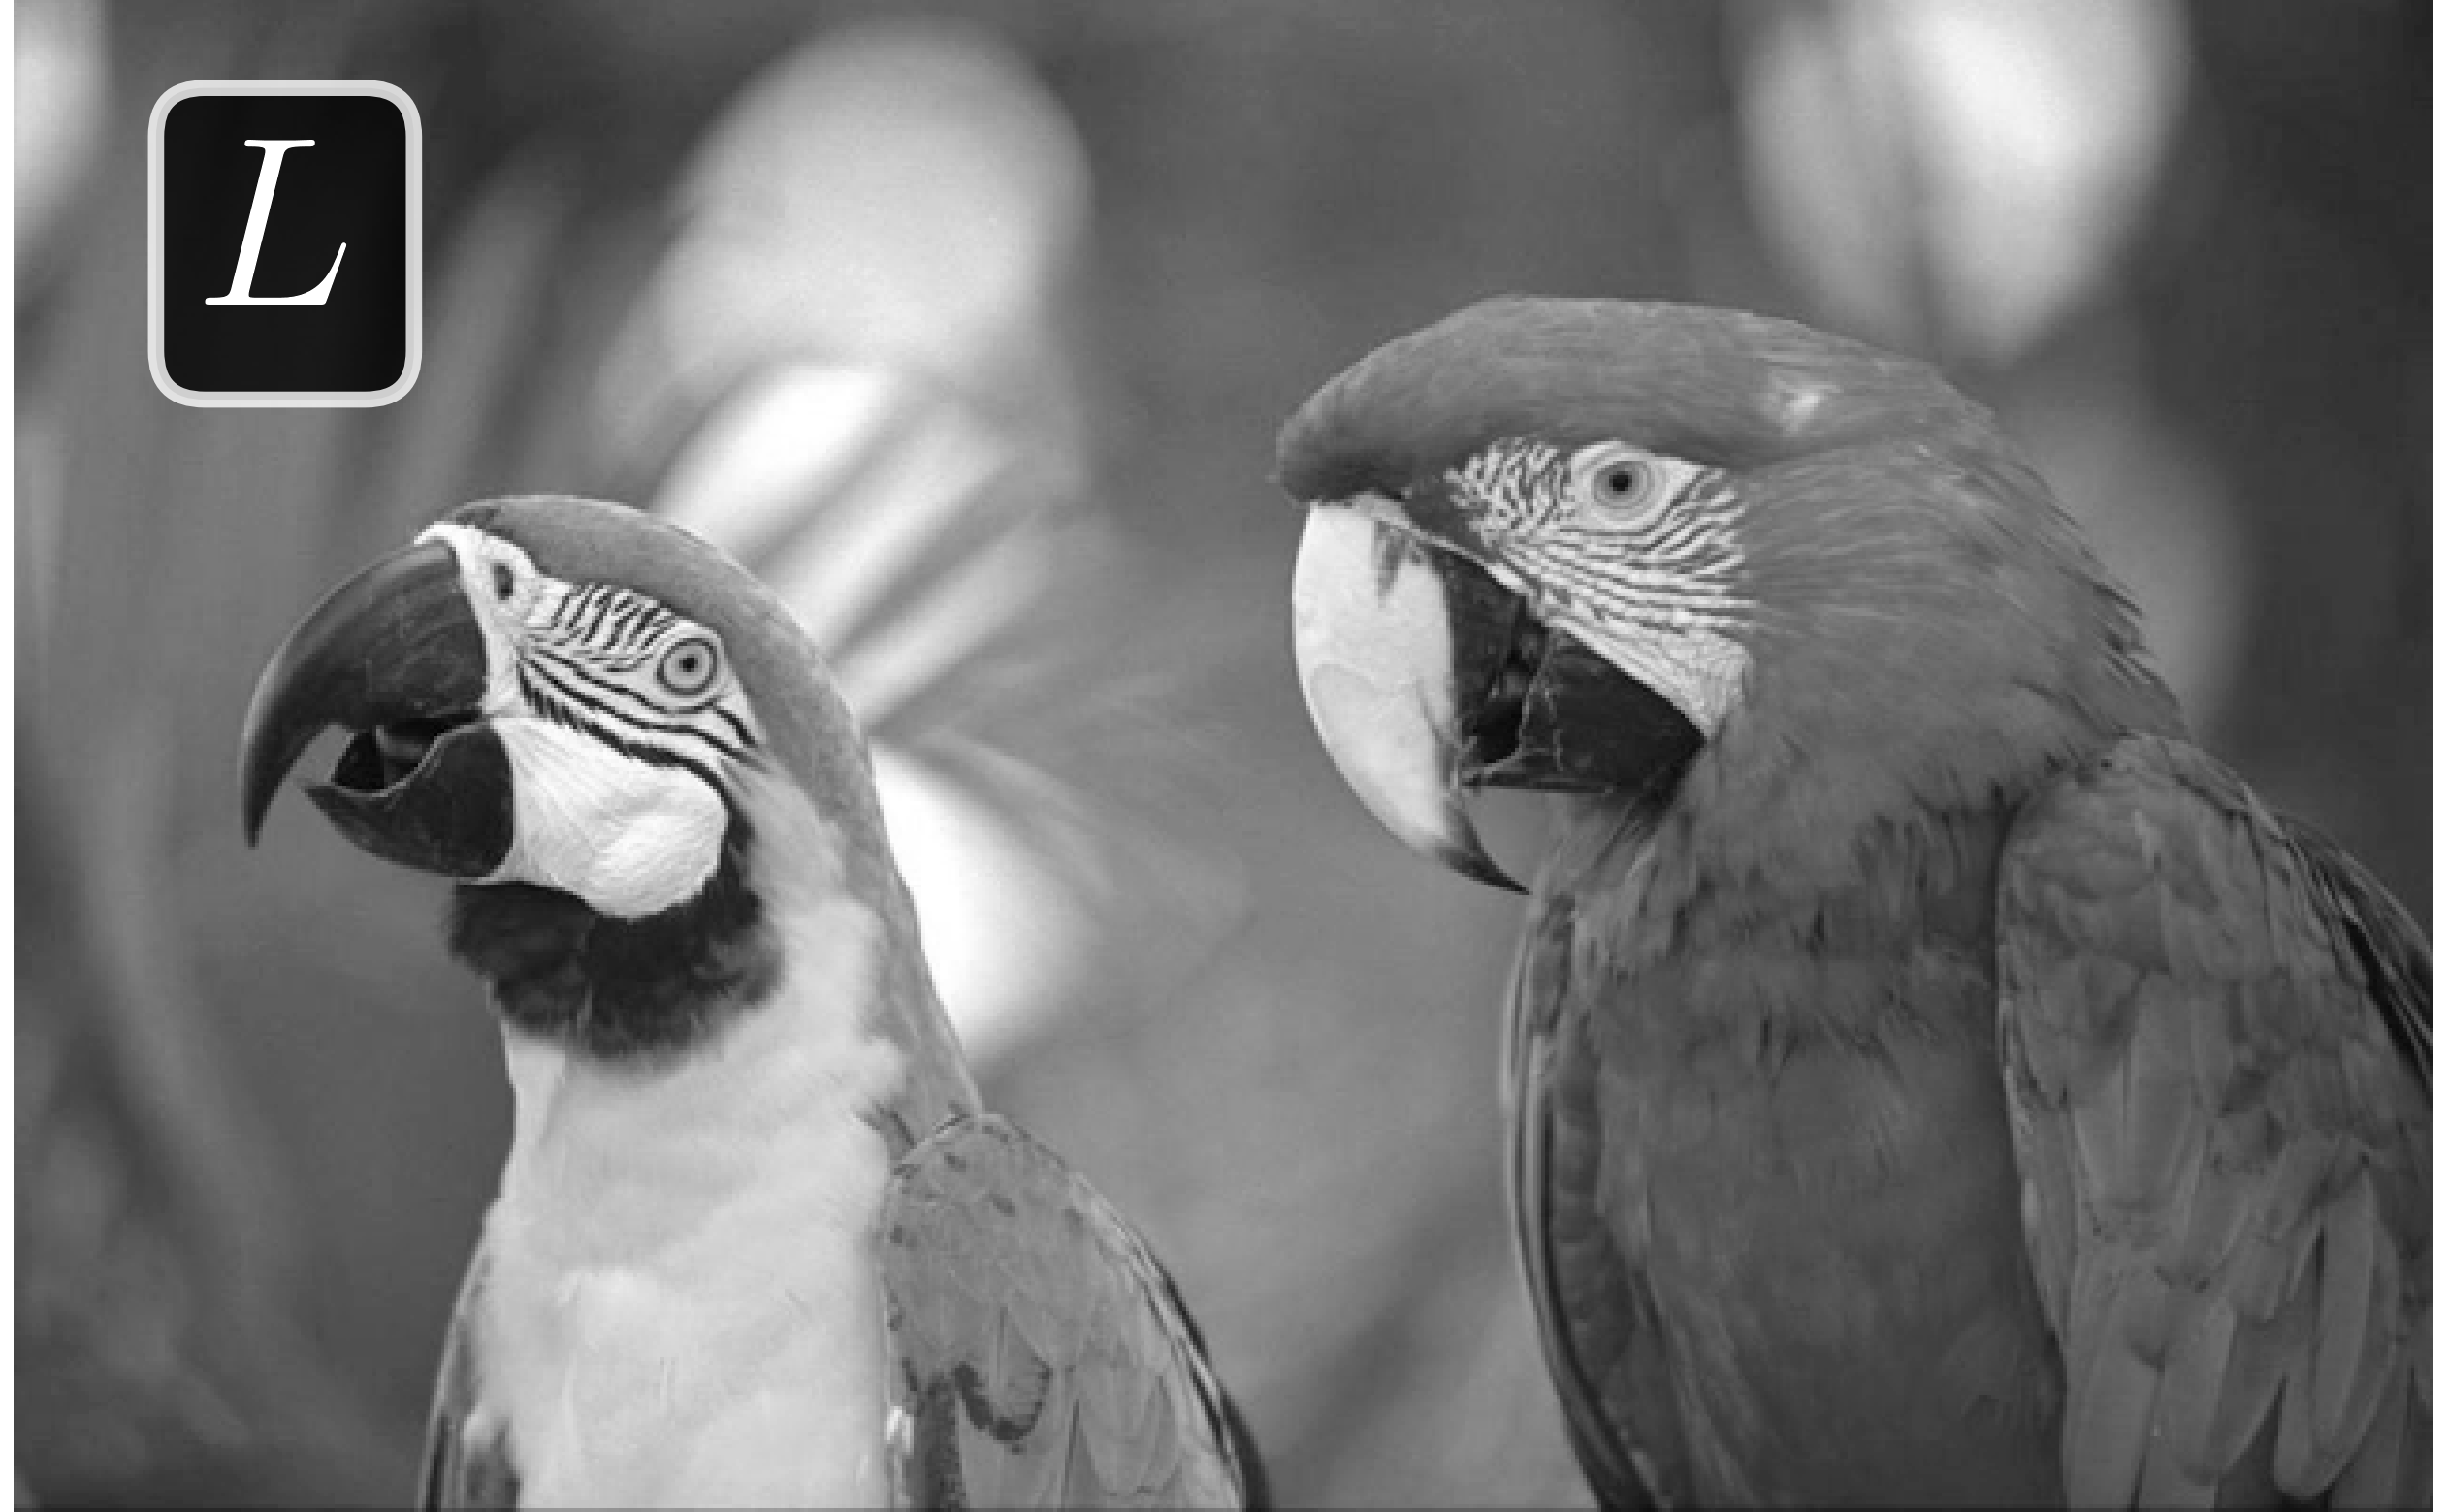
\includegraphics[width=\dimexpr\linewidth-20pt\relax]{araras_L}
    \end{subfigure}    
    ~ %add desired spacing between images, e. g. ~, \quad, \qquad, \hfill etc. 
      %(or a blank line to force the subfigure onto a new line)
    \begin{subfigure}[b]{0.3\textwidth}
        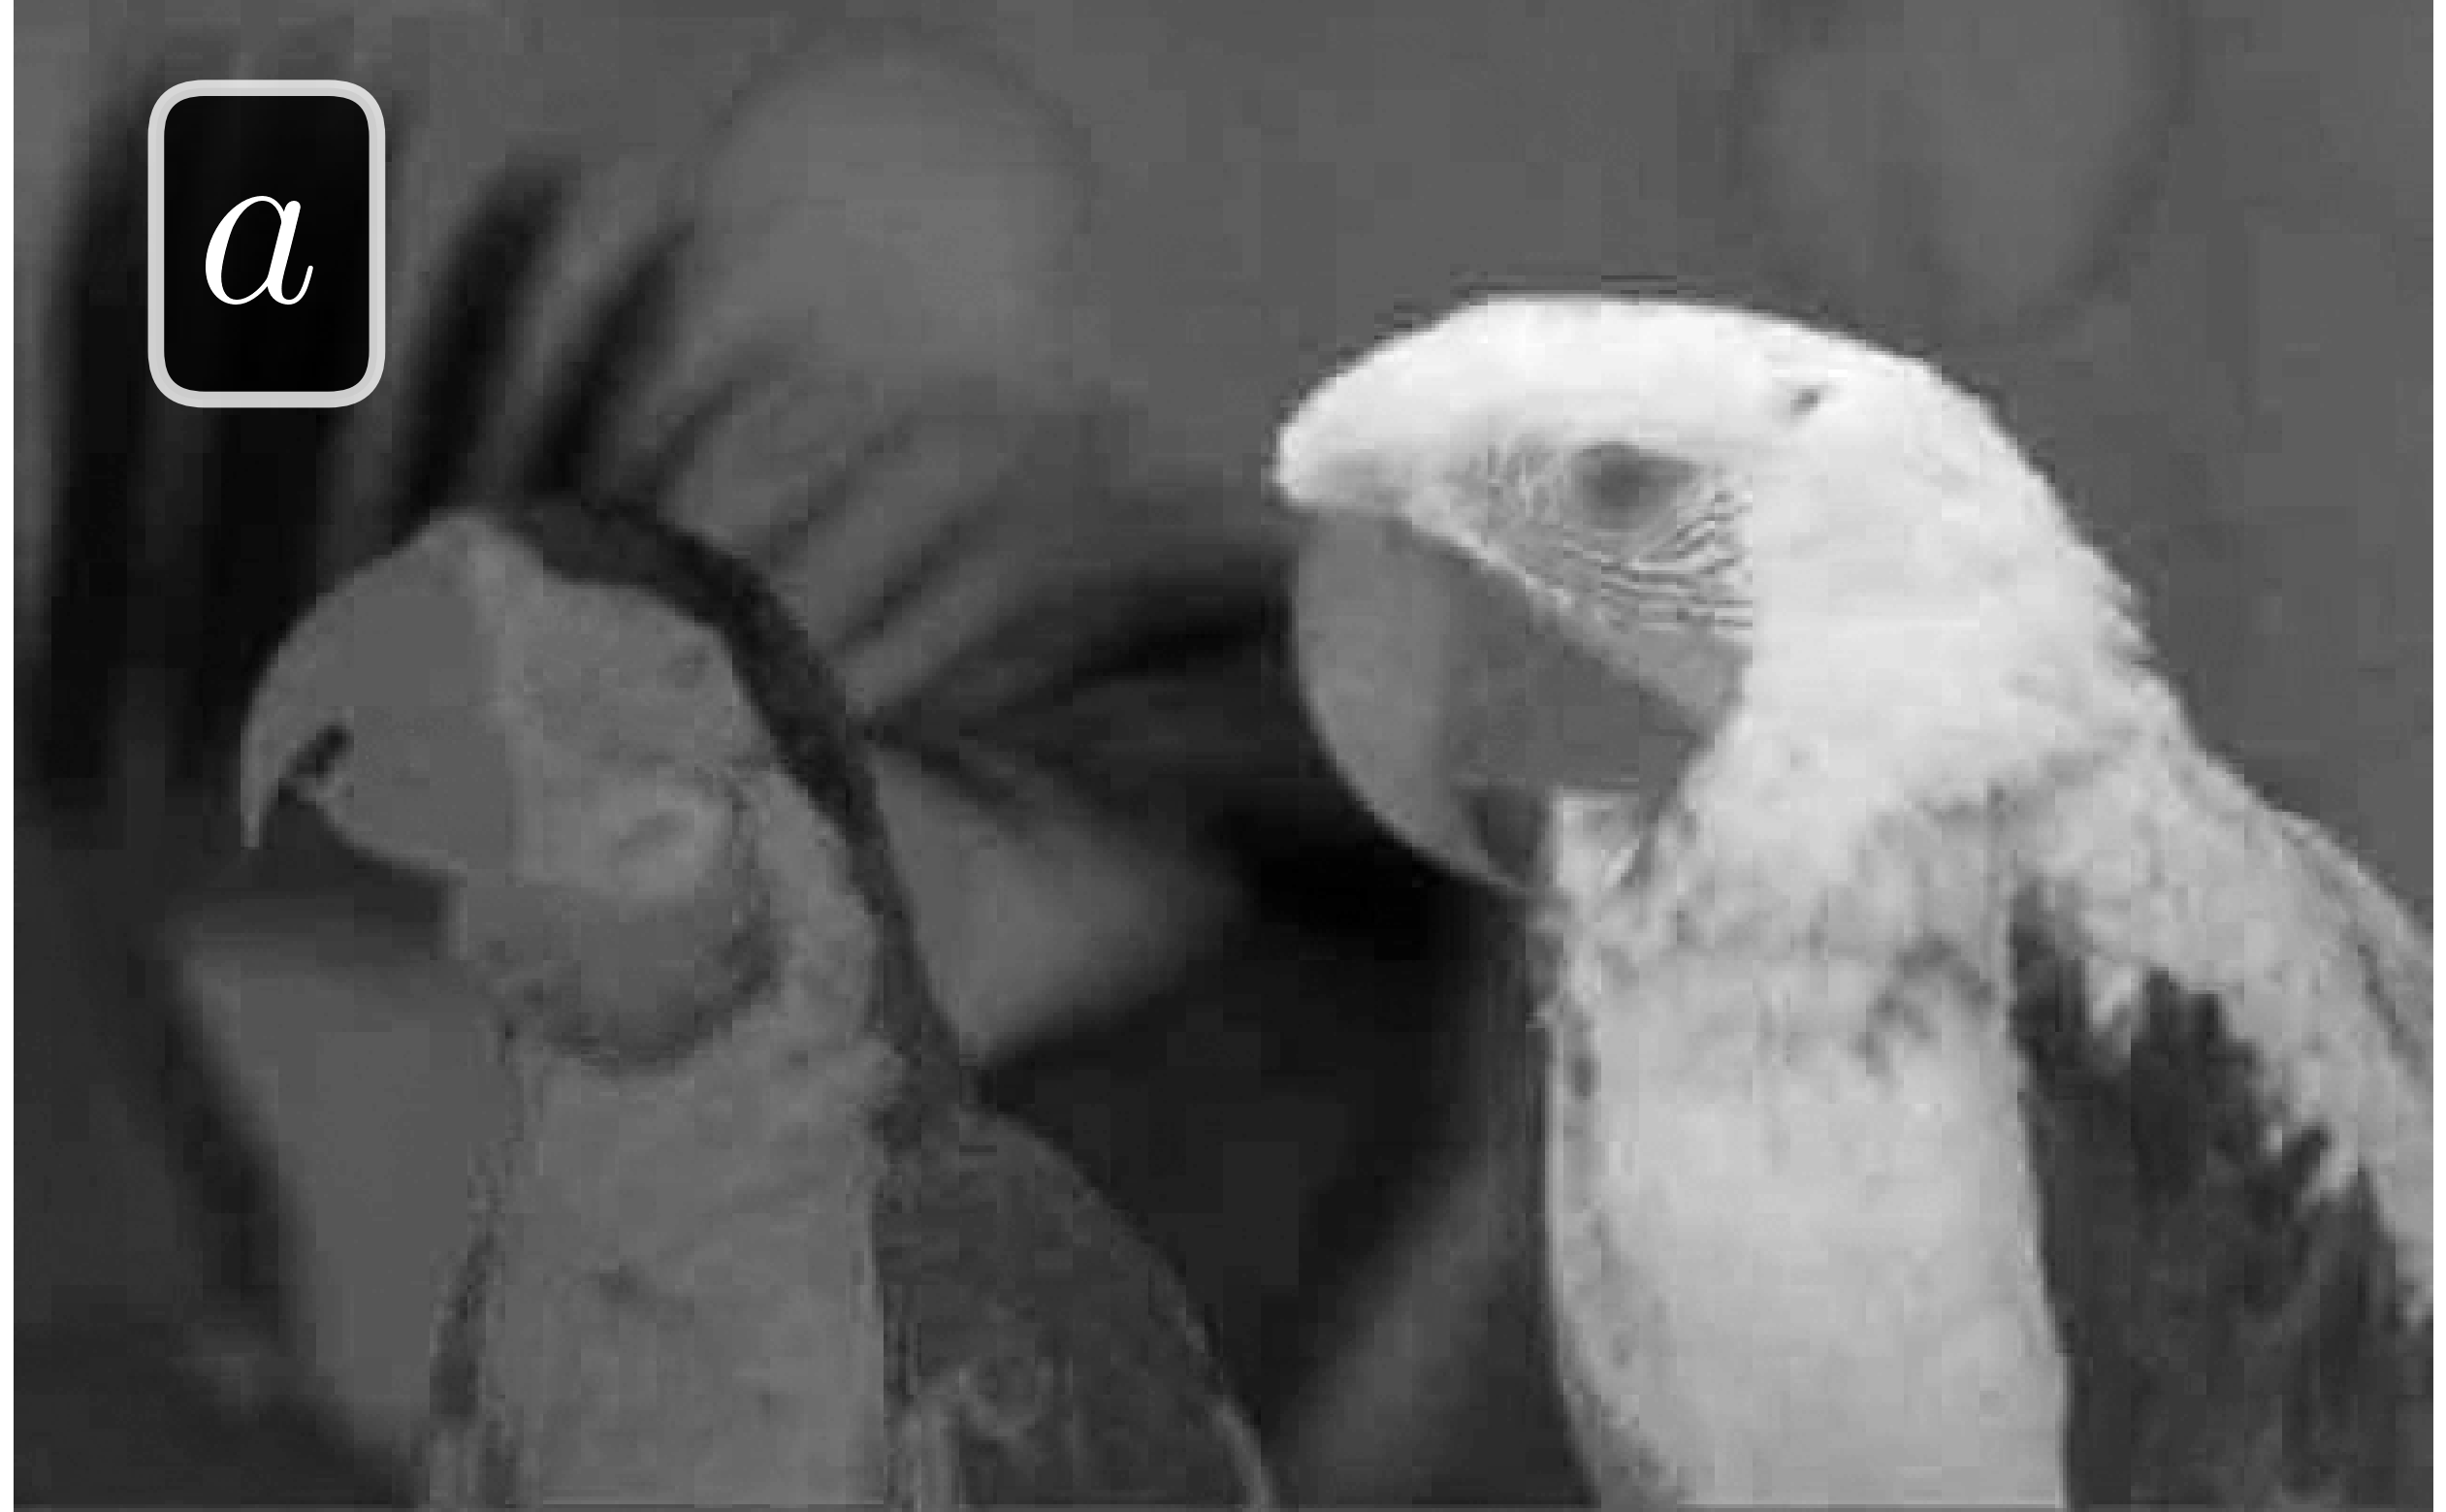
\includegraphics[width=\textwidth]{araras_a}
    \end{subfigure}
    ~ %add desired spacing between images, e. g. ~, \quad, \qquad, \hfill etc. 
      %(or a blank line to force the subfigure onto a new line)
    \begin{subfigure}[b]{0.3\textwidth}
        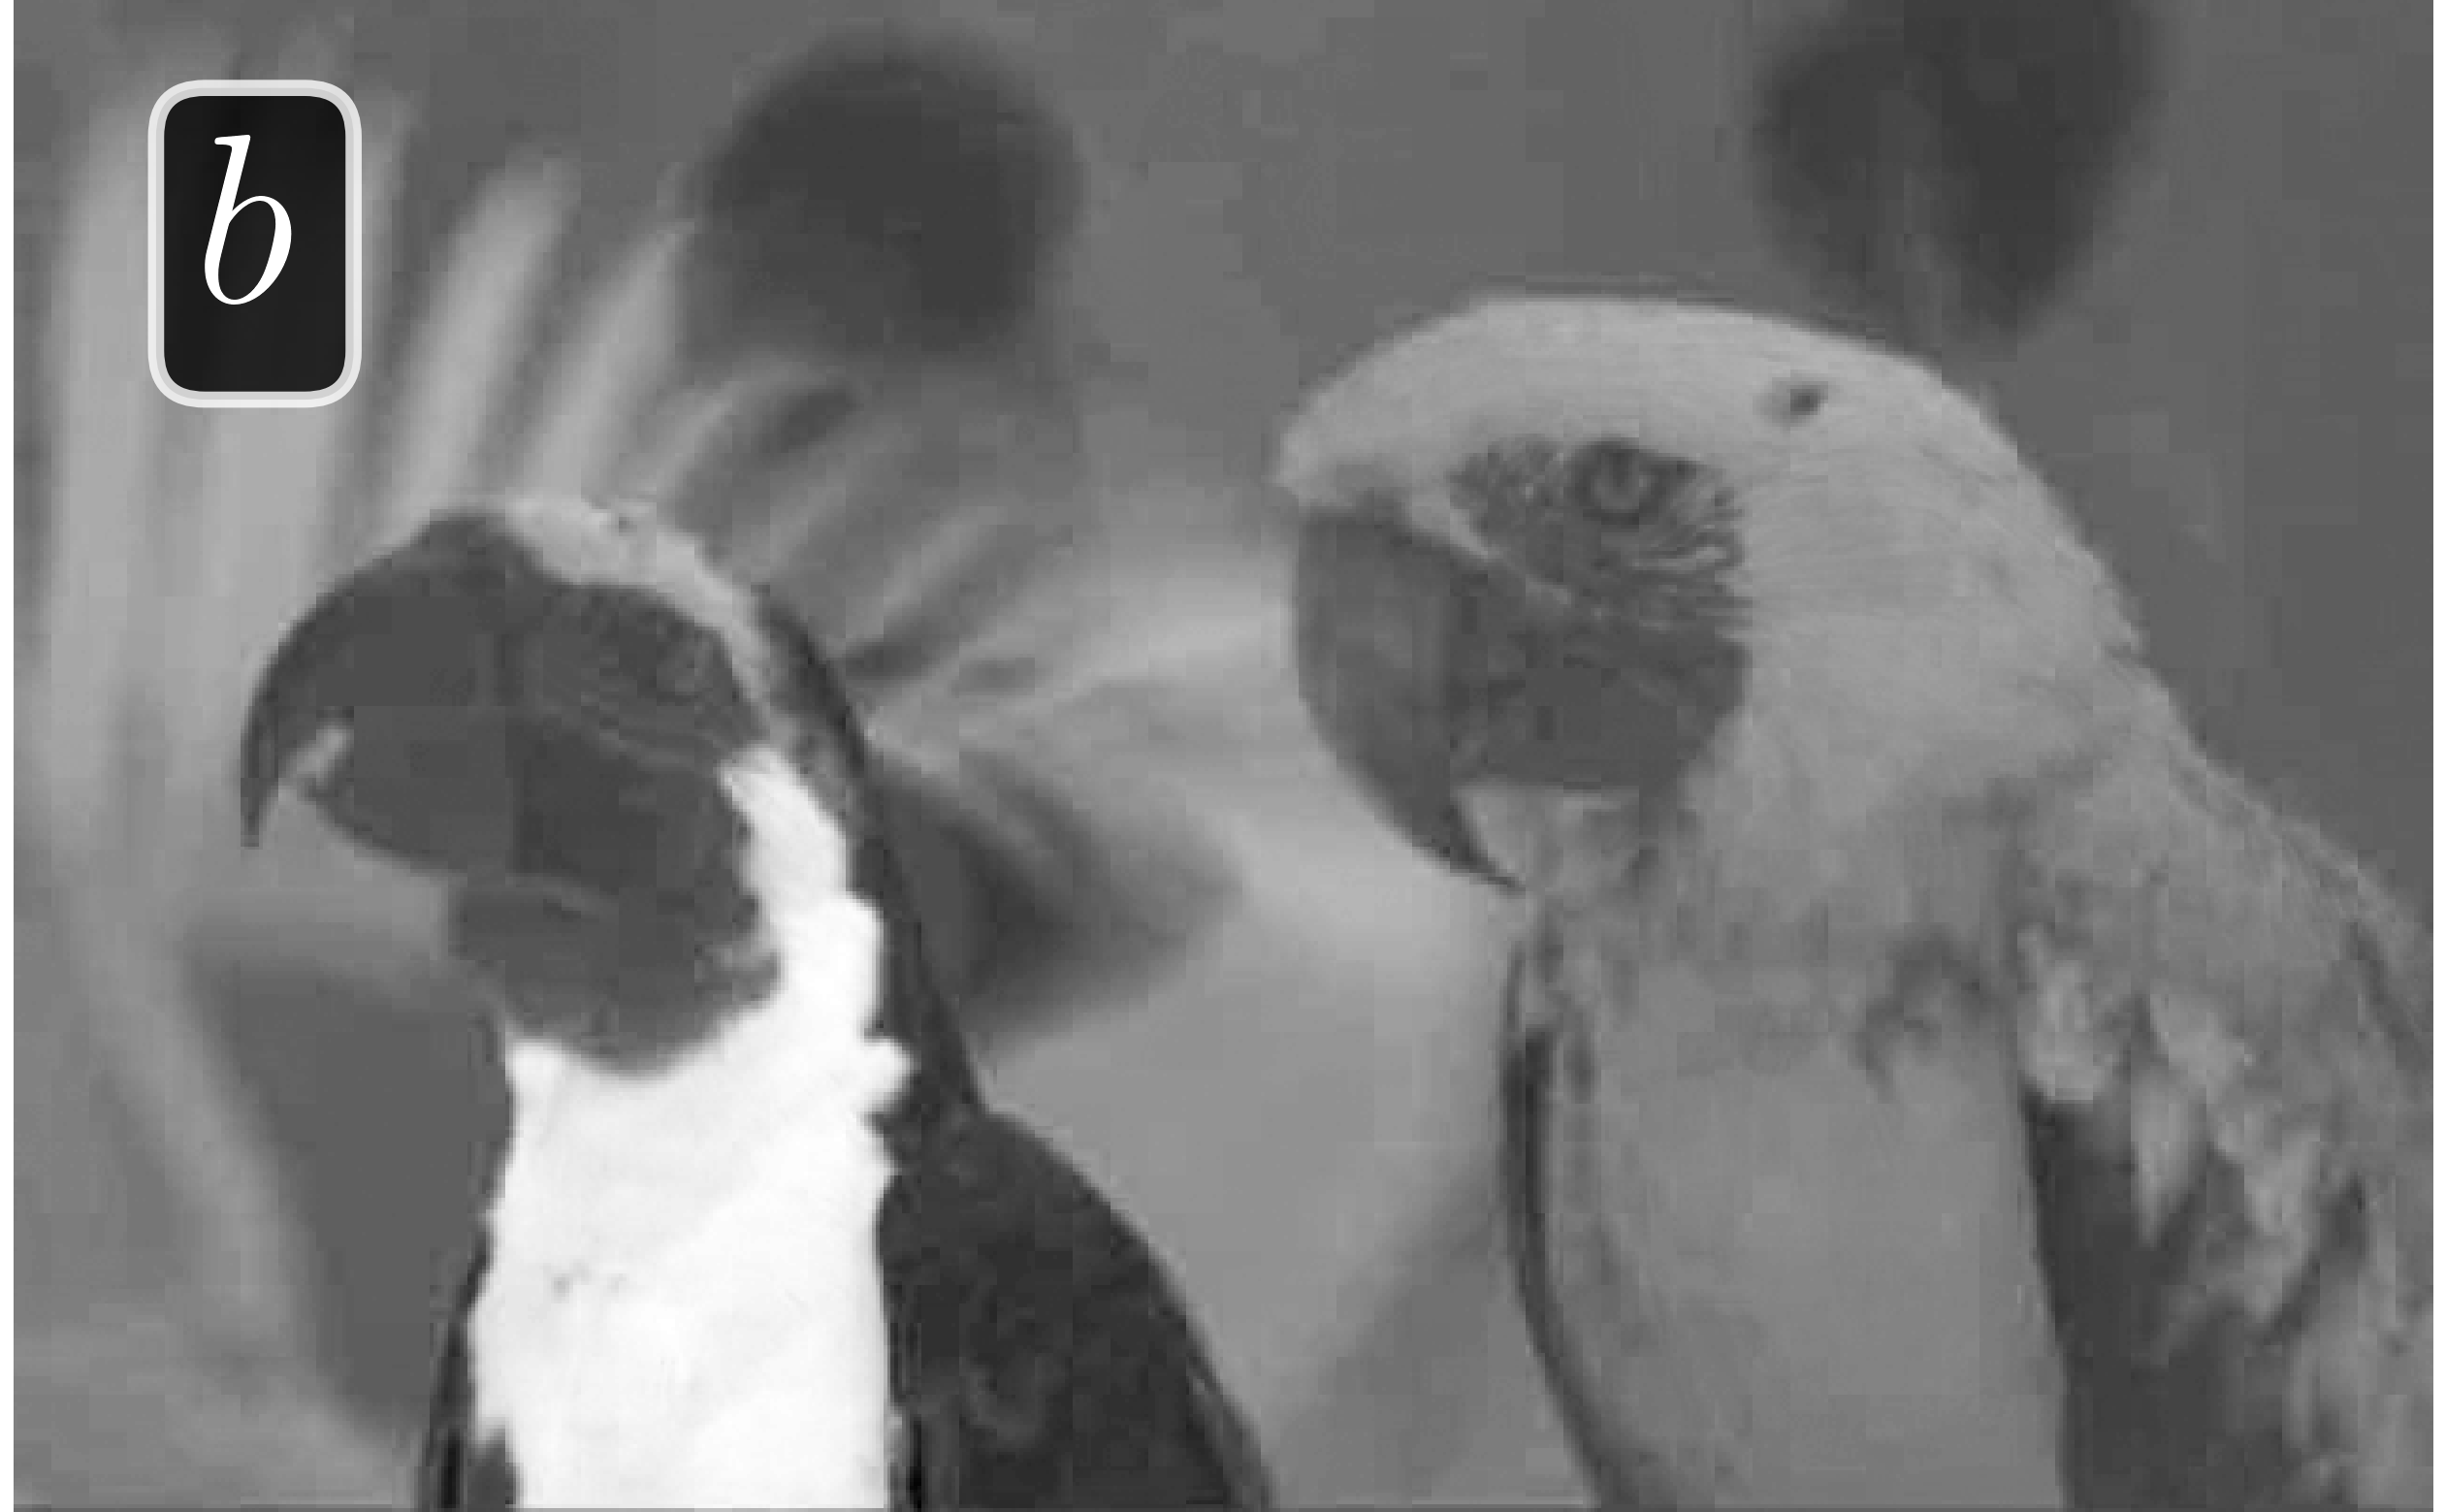
\includegraphics[width=\textwidth]{araras_b}
    \end{subfigure} 

	\caption{Color channels of an image in different color spaces in a grayscale}\label{fig:images_color_space}    
\end{figure}

The overall distribution of color within an image is a useful clue that contributes to the description of the content of an image. For example, we can characterize images that contain landscapes with mountains, jungles, urban environments, deserts or other scenes with different elements by their color distribution. The global color distribution can be represented by means of a color image histogram, which is a discrete function that associates to each intensity value (per color channel) the number of pixels that belong to this value.

The advantages of this representation is that they are invariant to the rotation or translation of the image, as well as, to a lesser extent, to changes of point of view and changes of scale. In addition, we can compact the image color information by reducing the count intervals, that is, by selecting a small number of bins.

\subsection{Single-channel Color Histogram}

\begin{figure}[!ht]
    \centering
    \begin{subfigure}[b]{0.45\textwidth}
        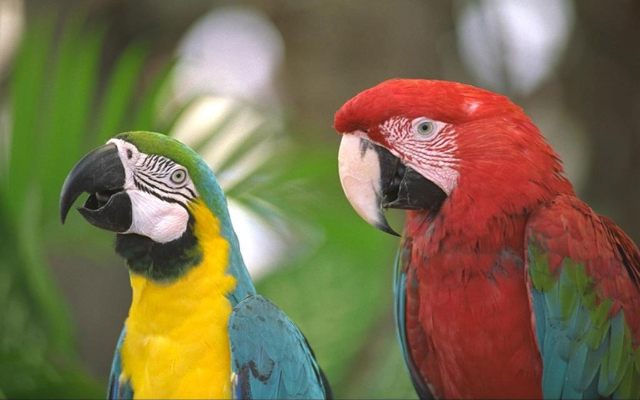
\includegraphics[width=\textwidth]{araras}
        \caption{Input image}
    \end{subfigure}
        ~ %add desired spacing between images, e. g. ~, \quad, \qquad, \hfill etc. 
      %(or a blank line to force the subfigure onto a new line)
    \begin{subfigure}[b]{0.45\textwidth}
        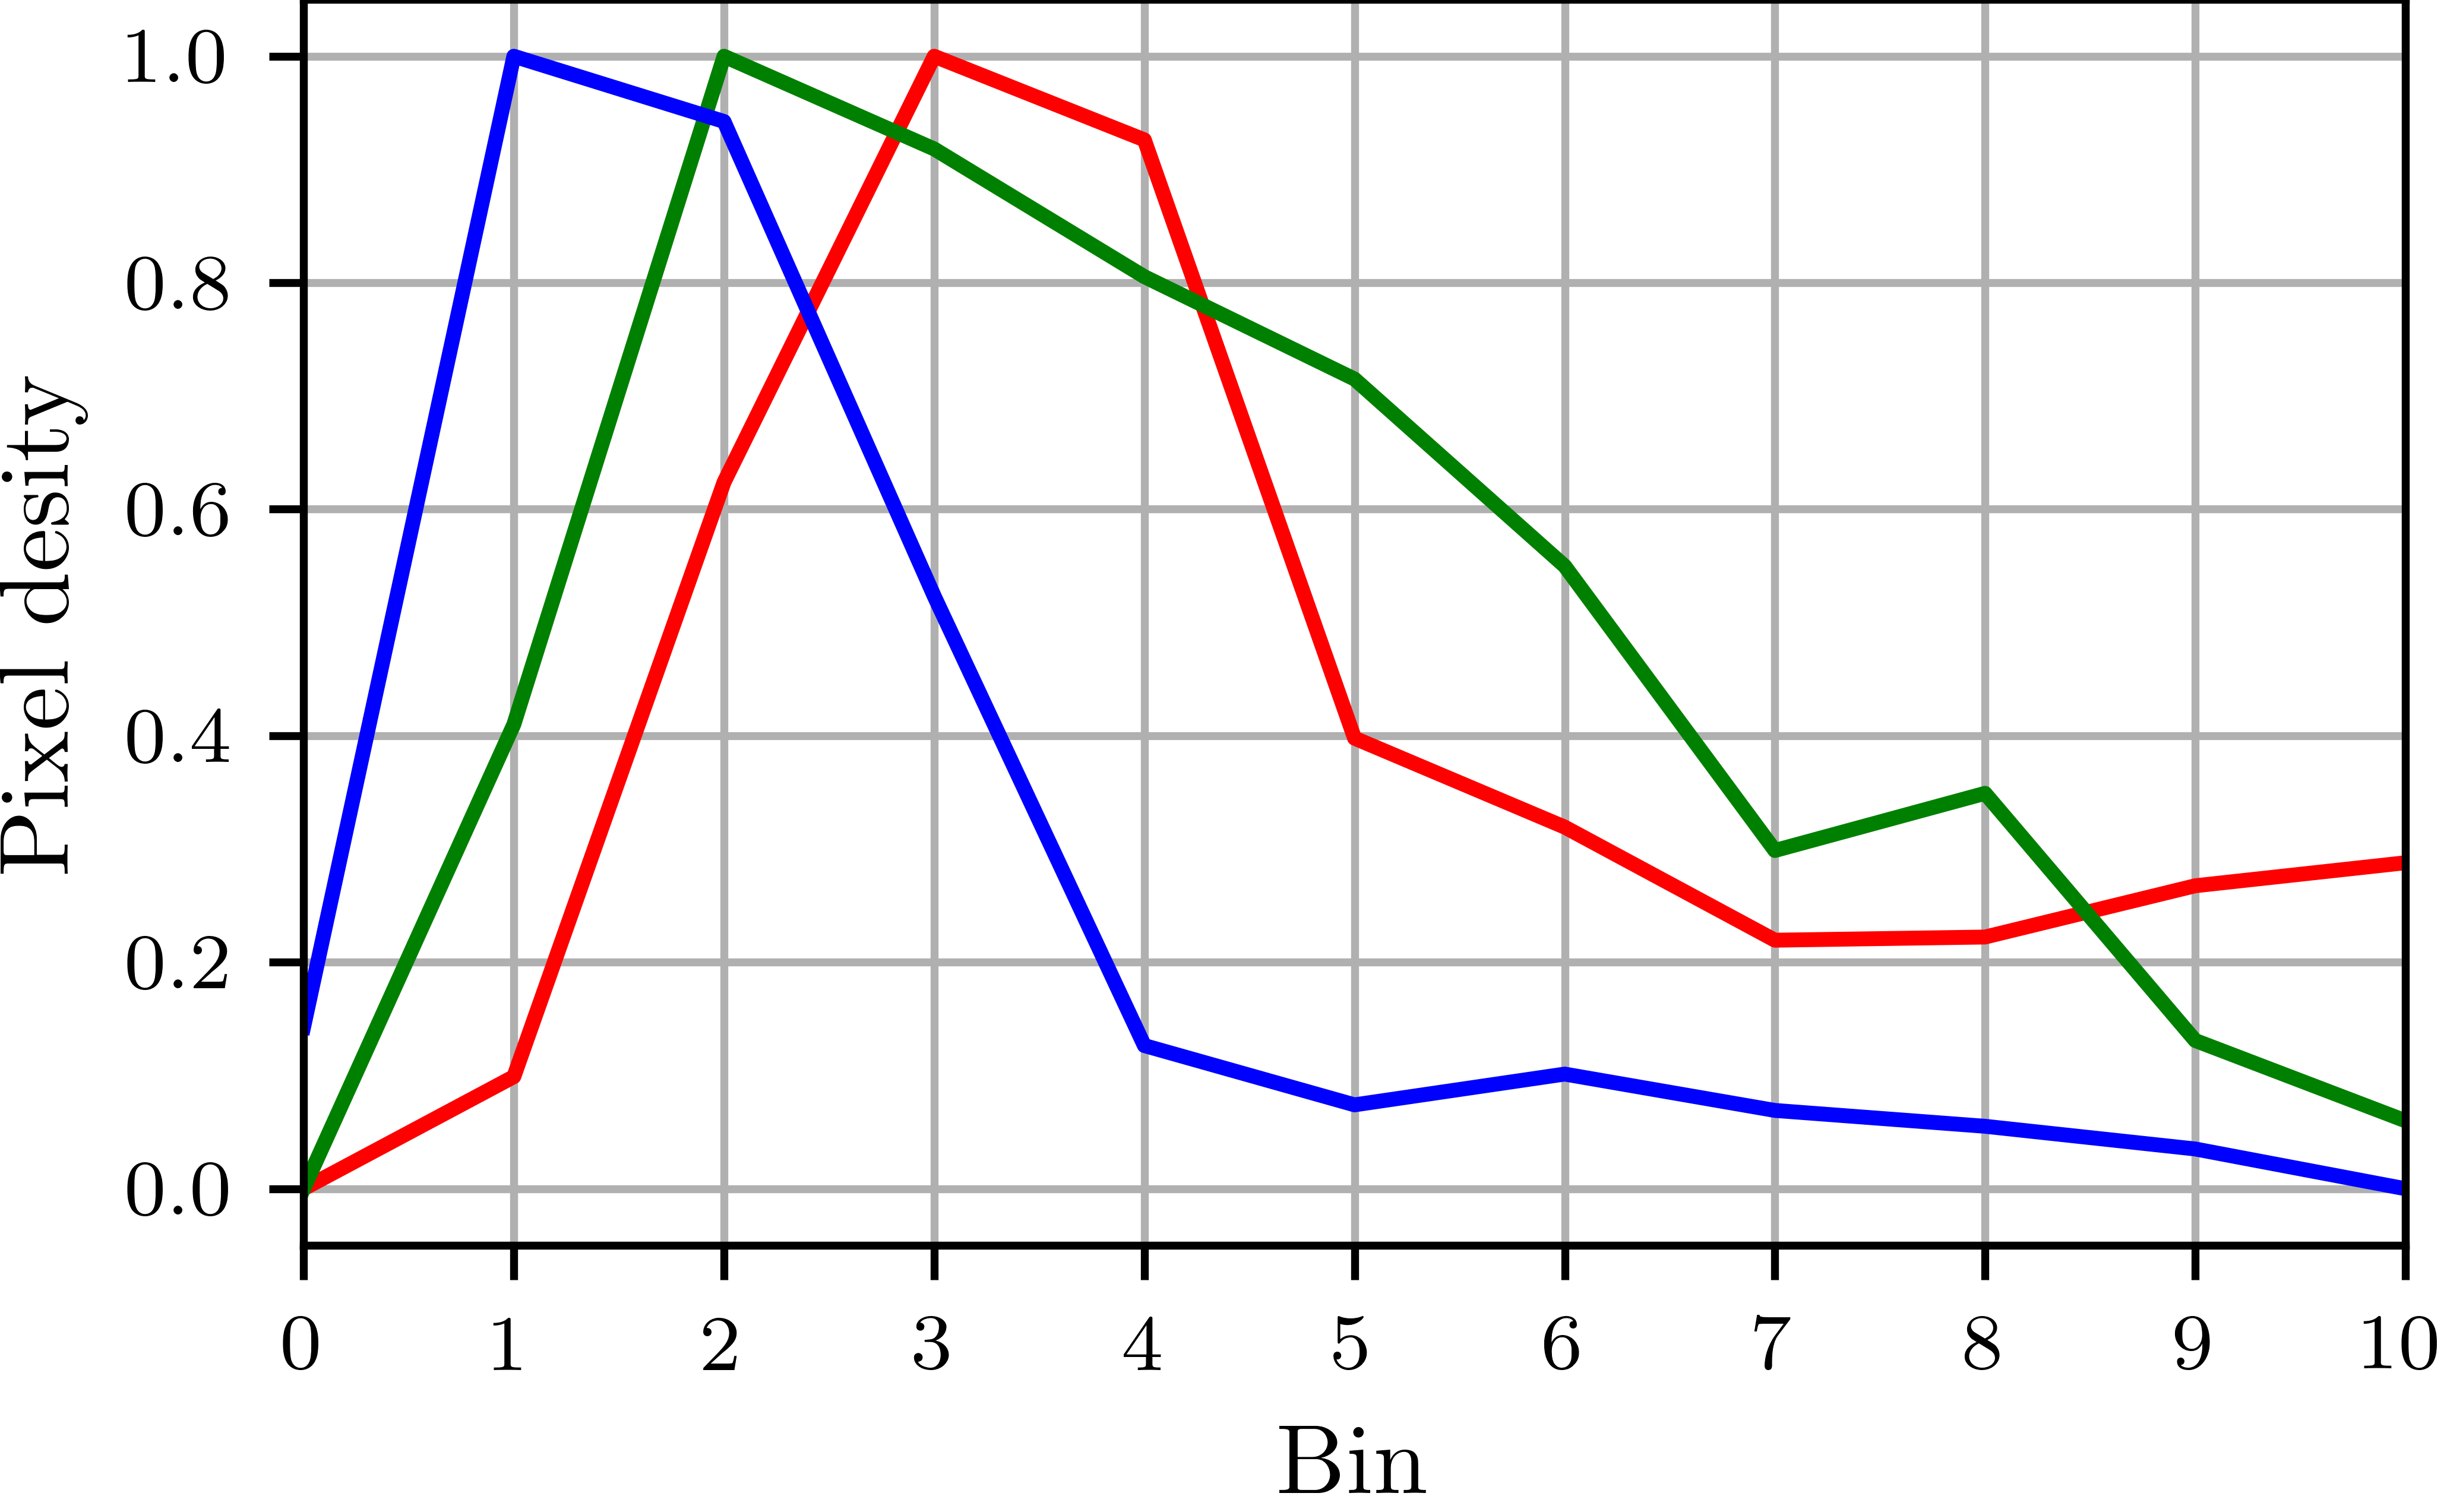
\includegraphics[width=\textwidth]{araras_single_histogram}
        \caption{Single-channel color pixel distribution}
    \end{subfigure} 
    
    \caption{}\label{fig:single_channel_histogram}    
\end{figure}
    
    
\subsection{3-d Color Histogram}

\begin{figure}[!ht]
    \centering
    \begin{subfigure}[b]{0.4\textwidth}
        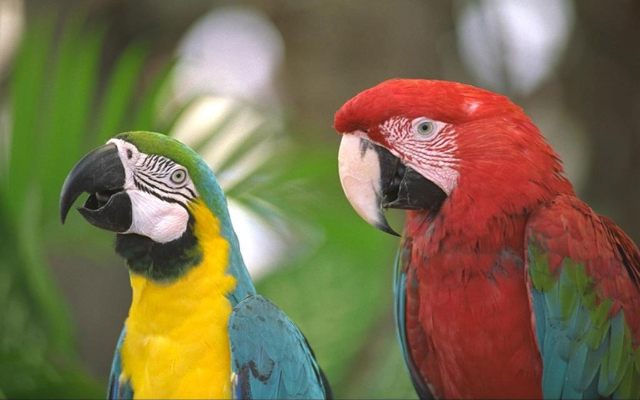
\includegraphics[width=\textwidth]{araras}
        \caption{Input image}
    \end{subfigure} \\
       
    \begin{subfigure}[b]{0.49\textwidth}
        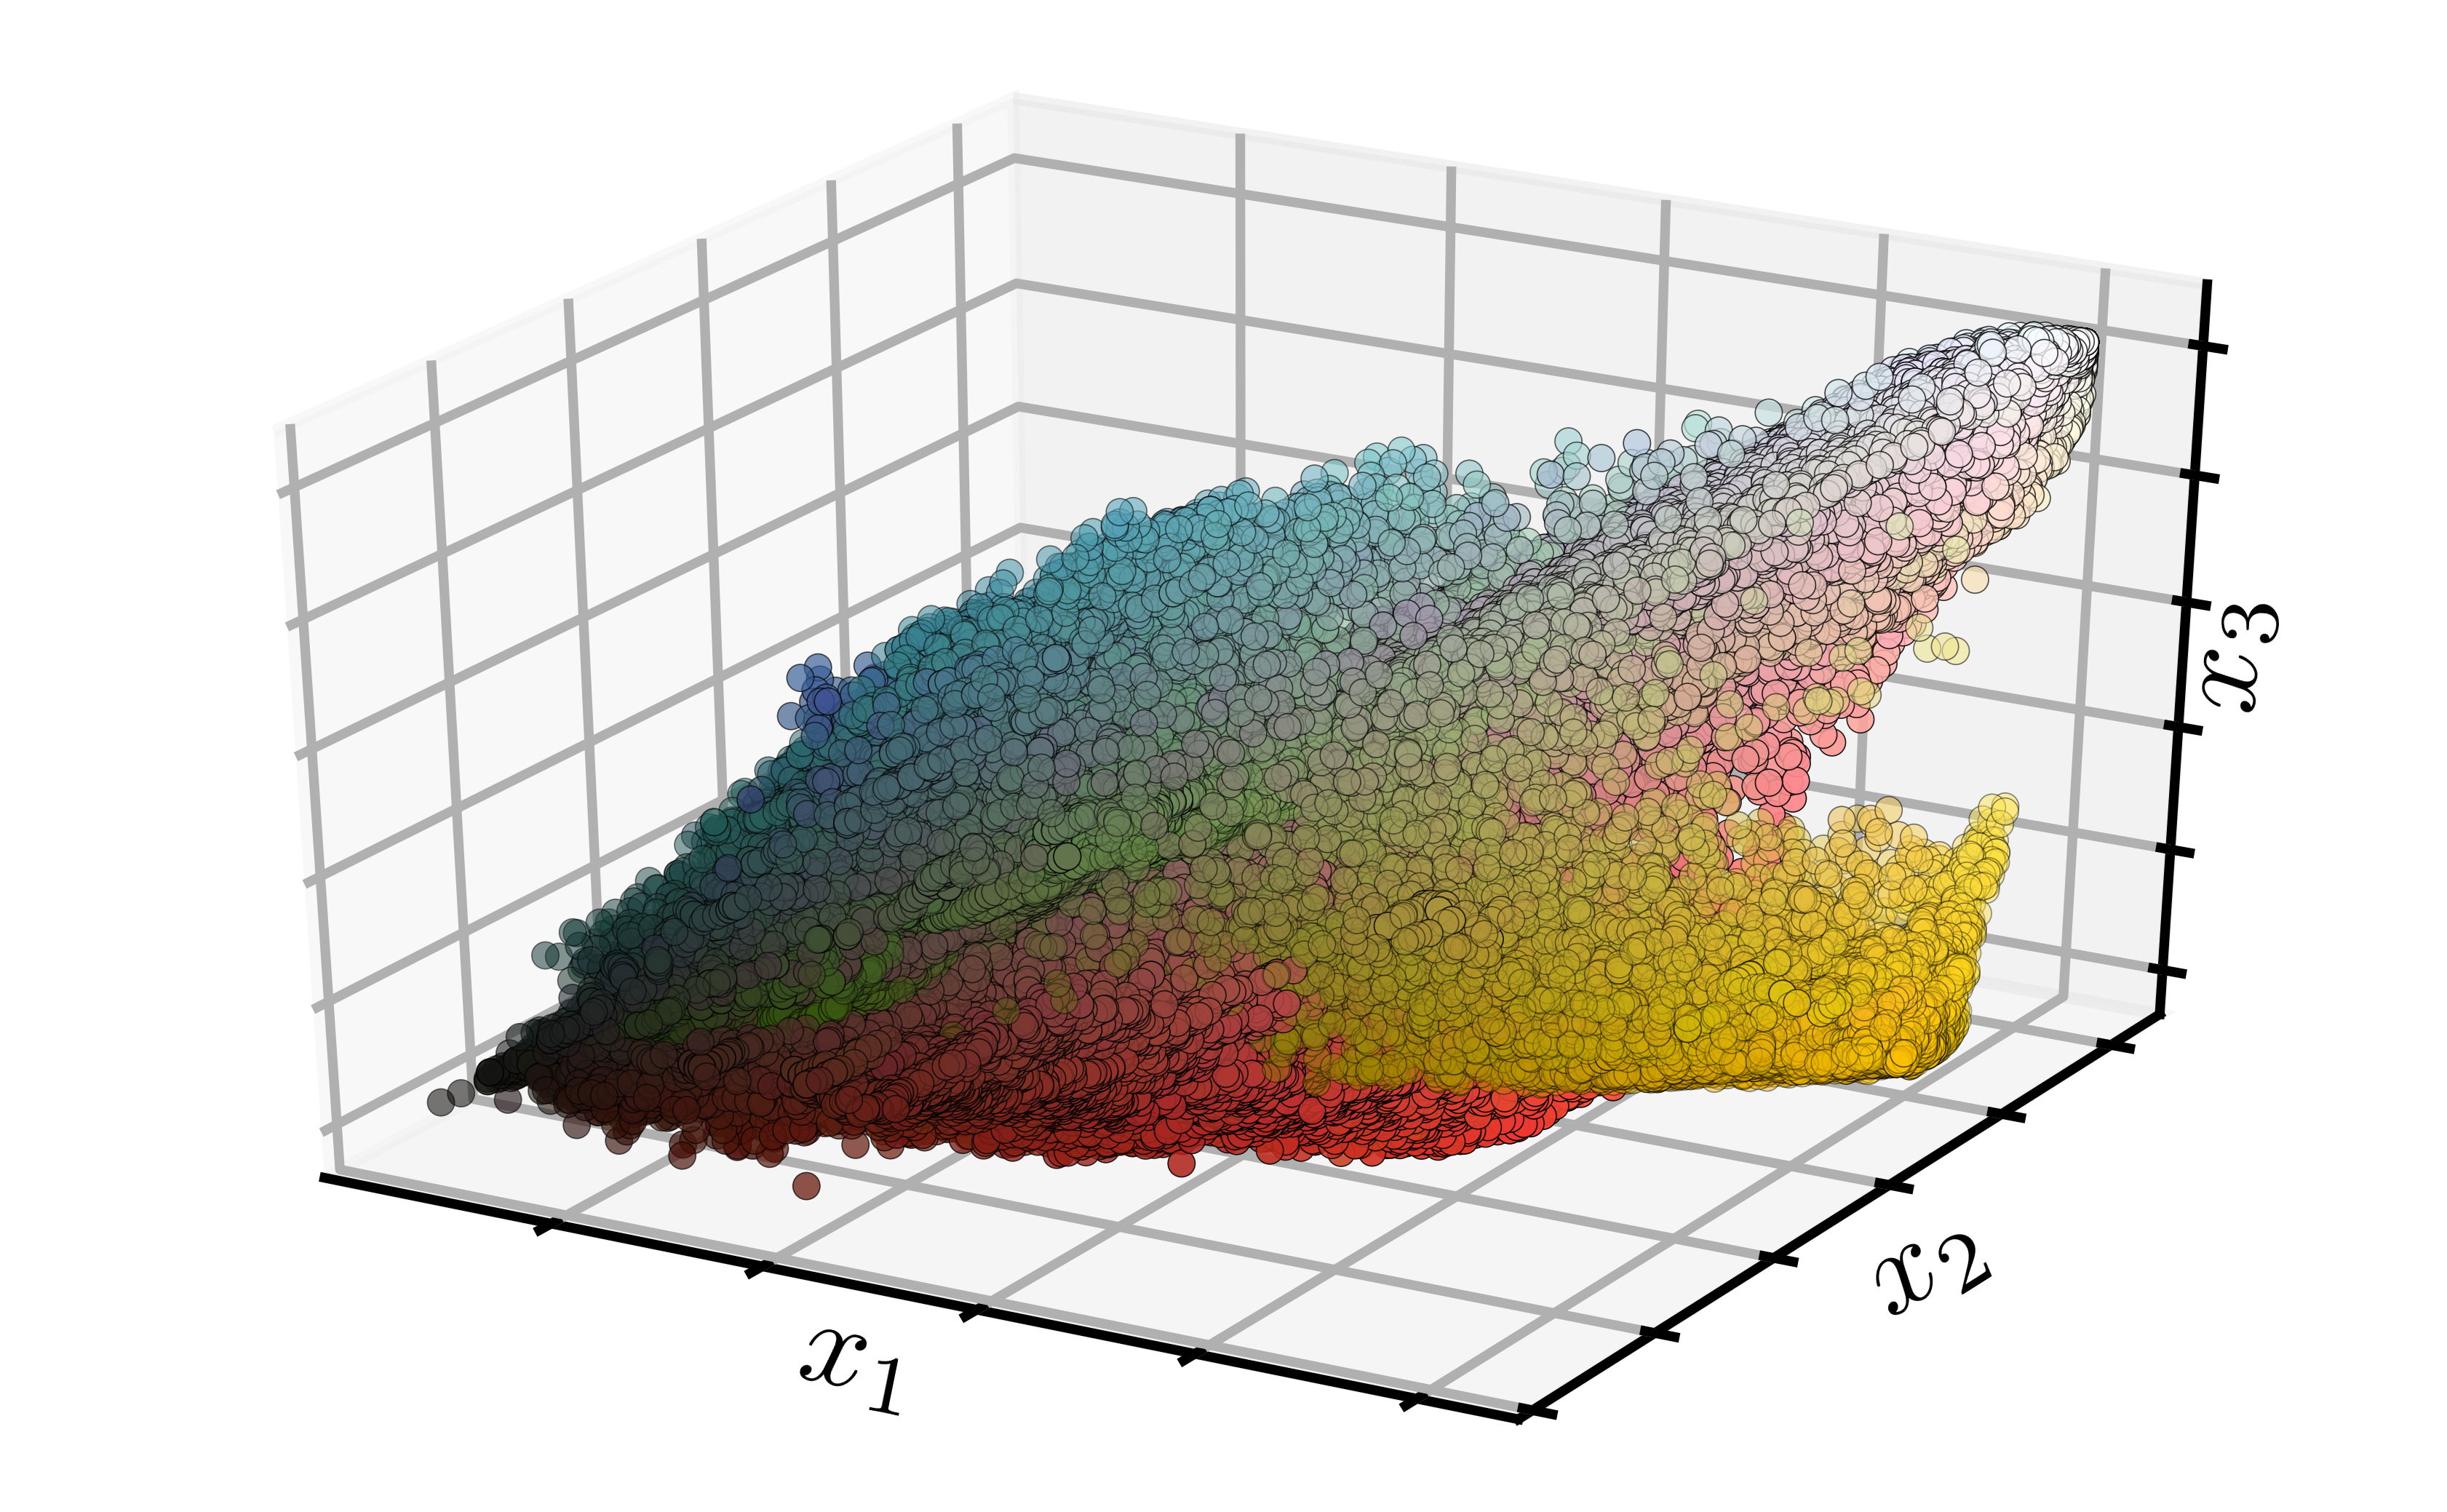
\includegraphics[width=\textwidth]{araras_3d_distribution}
        \caption{3-d image color pixel distribution}
    \end{subfigure} 
    \begin{subfigure}[b]{0.49\textwidth}
        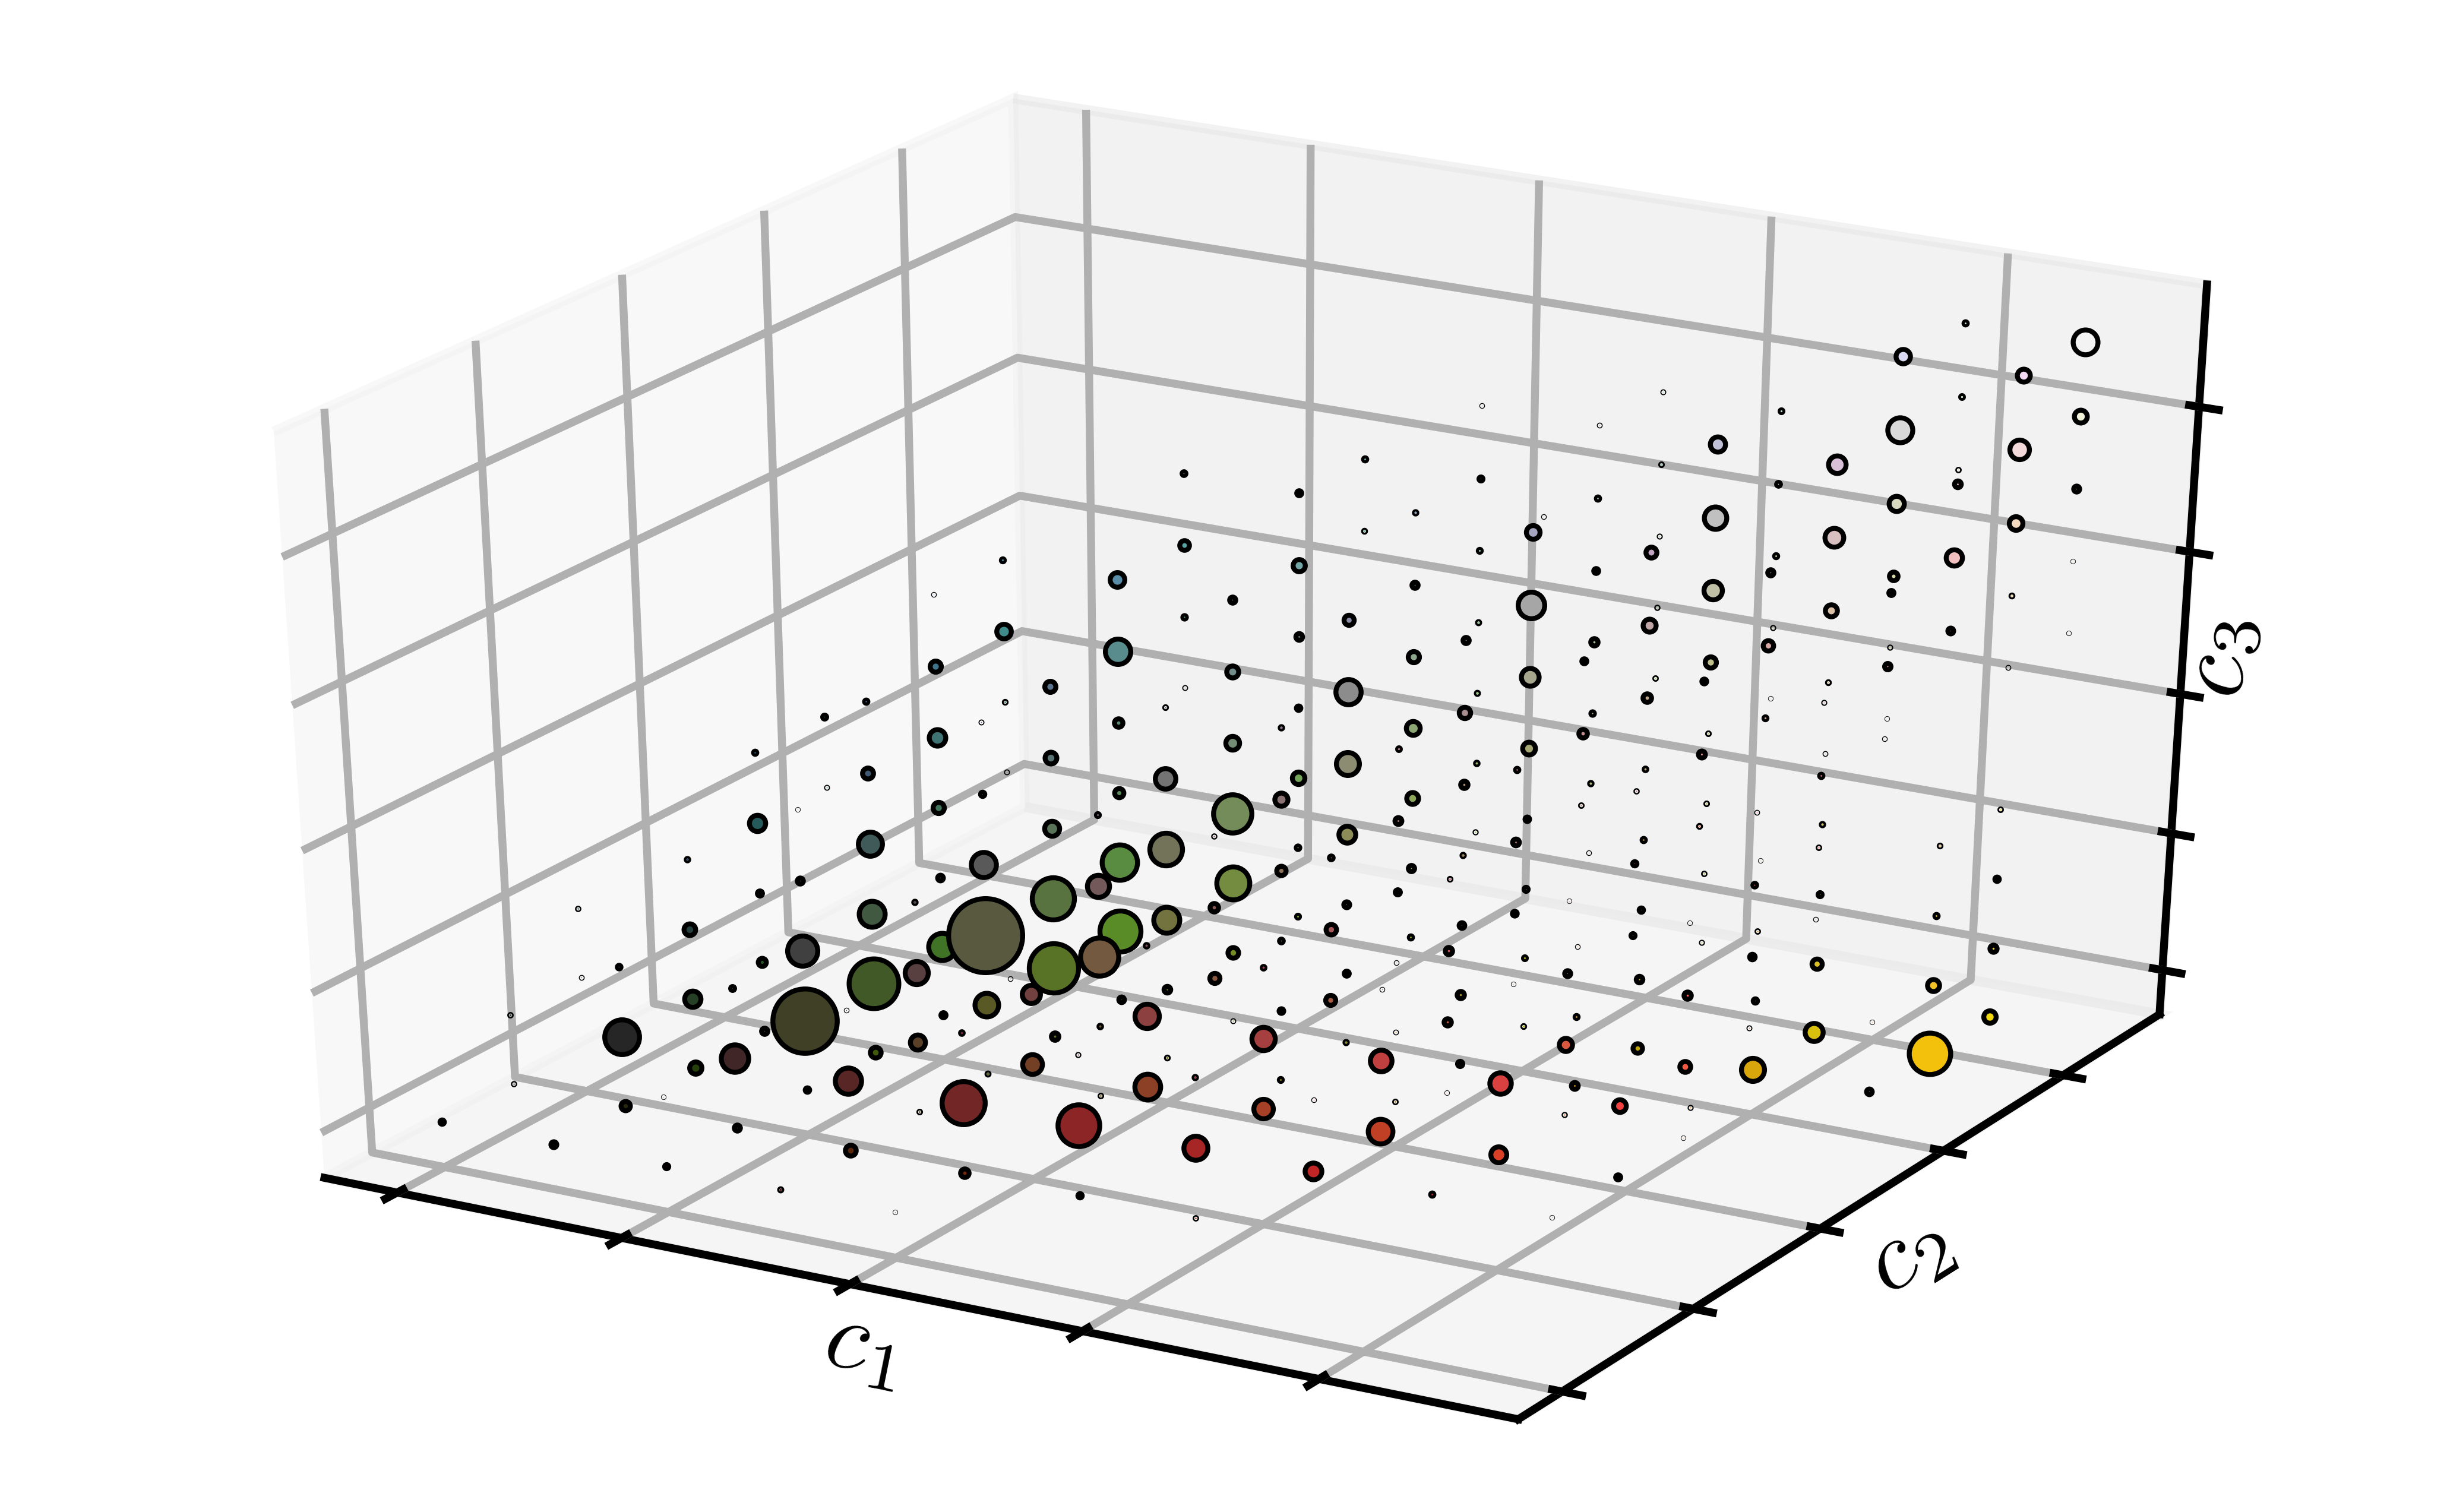
\includegraphics[width=\textwidth]{araras_3d_histogram}
        \caption{3-d color pixel histogram}
    \end{subfigure} 
    
    \caption{3-d image color representation. 3-d pixel distribution and 10 bins 3-d pixel histogram.}\label{fig:3d_color_representation}    
\end{figure}


\subsection{Color Signature}

\begin{figure}[!ht]
    \centering
    \begin{subfigure}[b]{0.4\textwidth}
        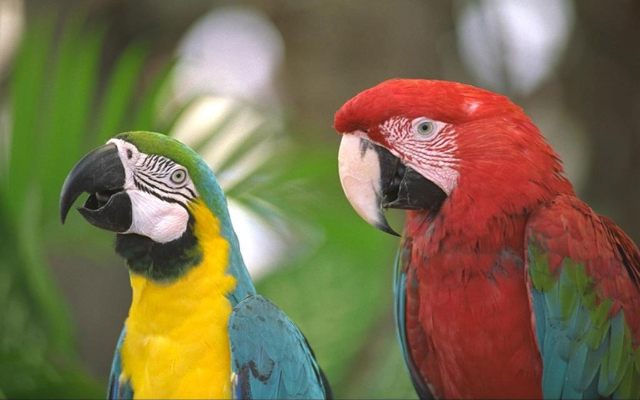
\includegraphics[width=\textwidth]{araras}
        \caption{Input image}
    \end{subfigure} \\
    
    \begin{subfigure}[b]{0.4\textwidth}
    	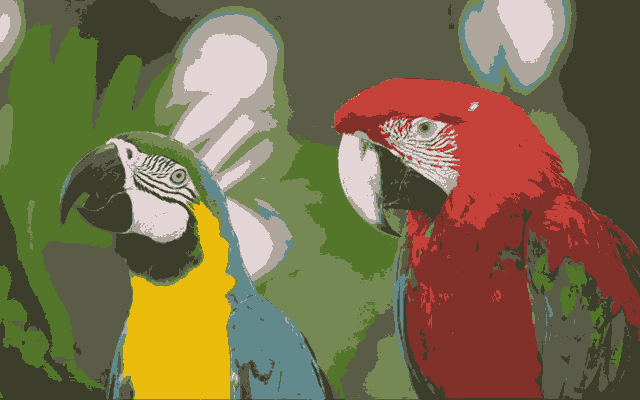
\includegraphics[width=\textwidth]{araras_color_clusters}
        
\includegraphics[width=\textwidth]{araras_bar_signature}
        \caption{Color signature}
    \end{subfigure}
    	~ %add desired spacing between images, e. g. ~, \quad, \qquad, \hfill etc. 
      %(or a blank line to force the subfigure onto a new line)
    \begin{subfigure}[b]{0.5\textwidth}
        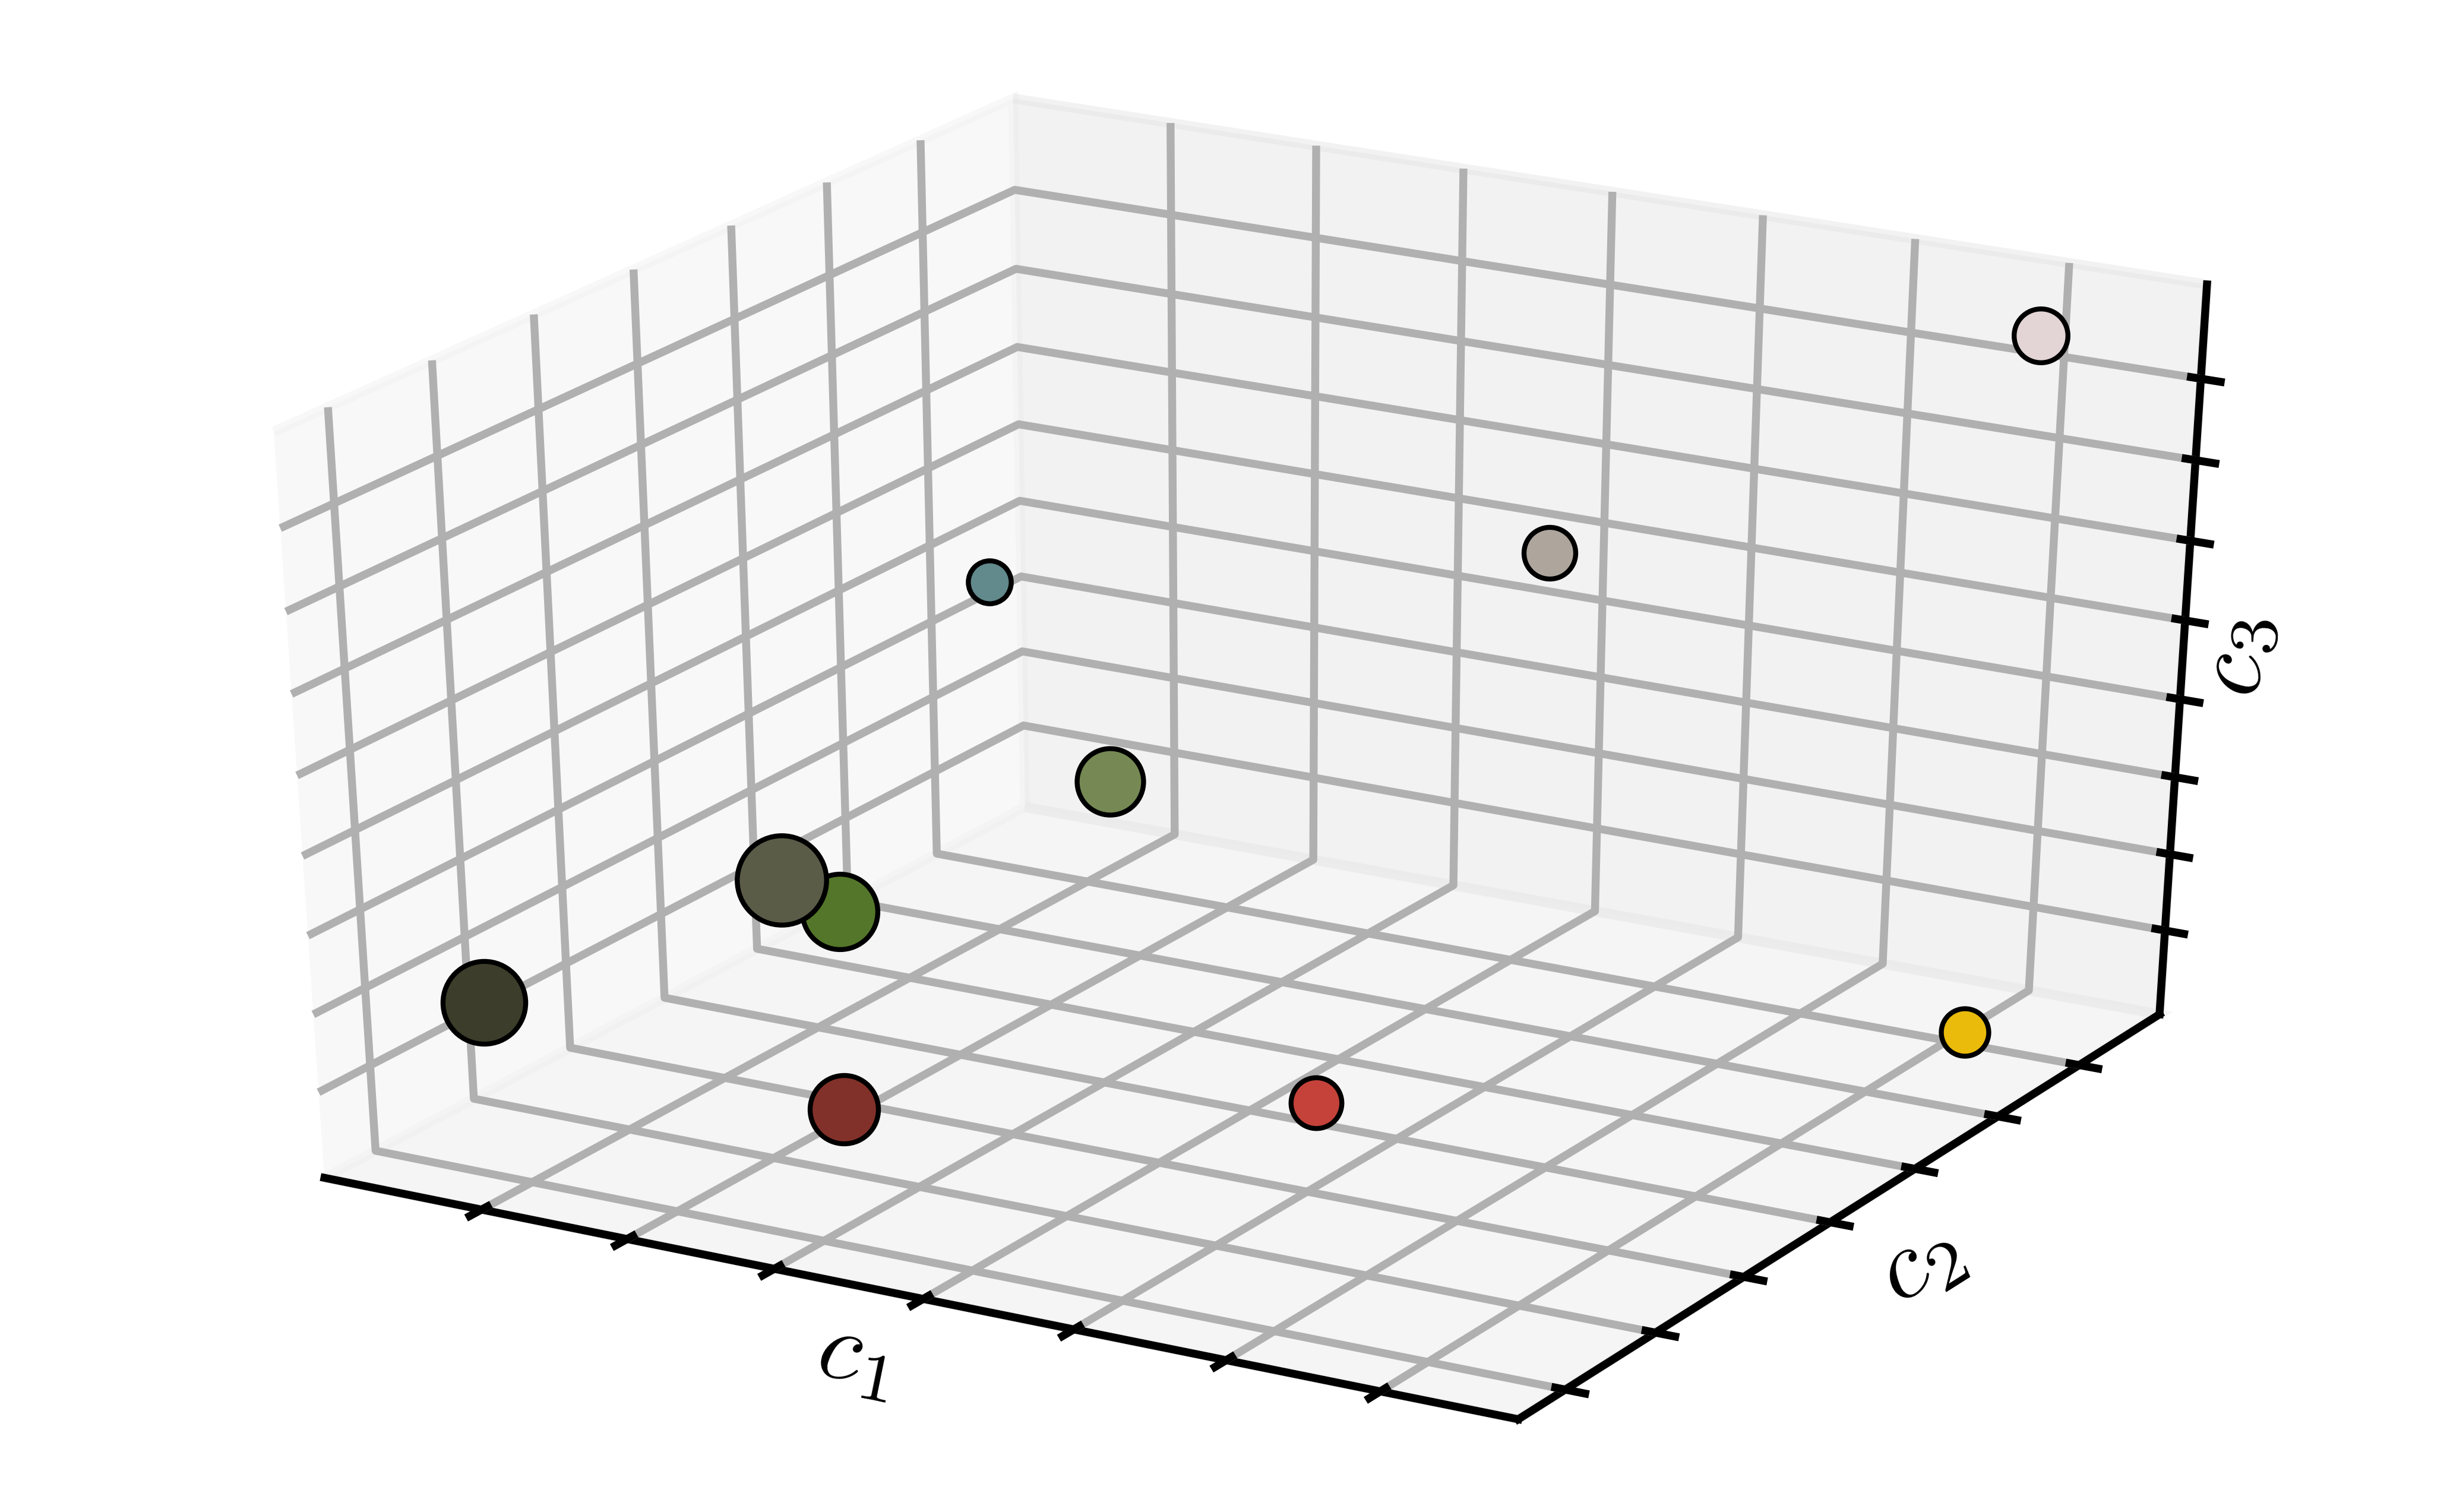
\includegraphics[width=\textwidth]{araras_3d_signature}
        \caption{3-d representation of color ignature}
    \end{subfigure} 
    	    
    \caption{Image color signature and the 3-d visualization of signature clusters.}\label{fig:color_signature}    
\end{figure}



\begin{figure}[!ht]
    \centering
    \begin{subfigure}[t]{\dimexpr0.32\textwidth+20pt\relax}
    	\makebox[20pt]{\raisebox{40pt}{ \small\textbf{\textsf{(a)}} }}%
    	
\includegraphics[width=\dimexpr\linewidth-20pt\relax]{tempo}
    \end{subfigure}~ 
%    \begin{subfigure}[b]{0.32\textwidth}
%        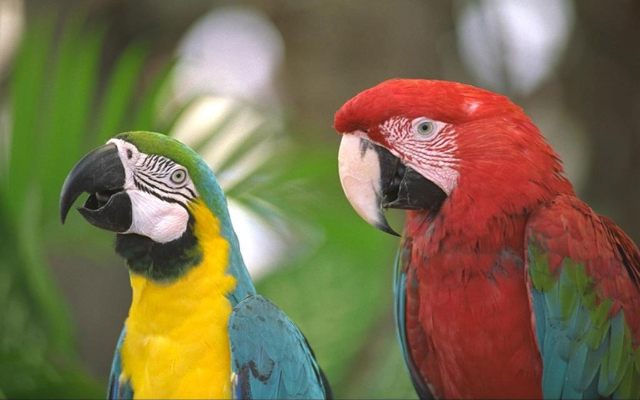
\includegraphics[width=\textwidth]{araras}
%    \end{subfigure}~
    \begin{subfigure}[b]{0.32\textwidth}
        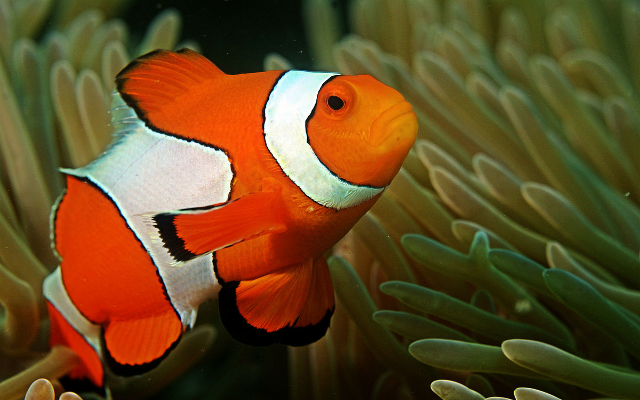
\includegraphics[width=\textwidth]{clownfish}
    \end{subfigure}~
    \begin{subfigure}[b]{0.32\textwidth}
        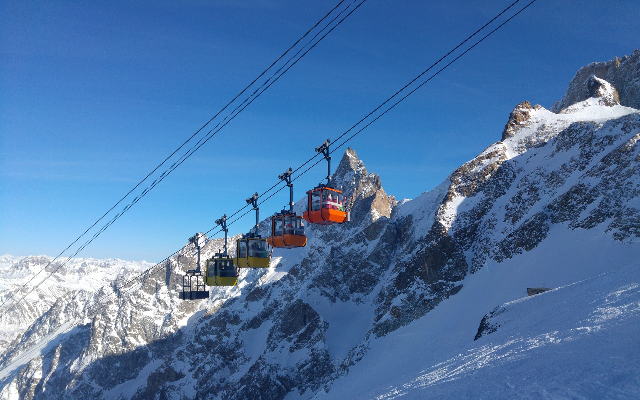
\includegraphics[width=\textwidth]{mountain}
    \end{subfigure}\vspace{10pt}
    
    \begin{subfigure}[t]{\dimexpr0.32\textwidth+20pt\relax}
    	\makebox[20pt]{\raisebox{40pt}{ \small\textbf{\textsf{(b)}} }}%
    	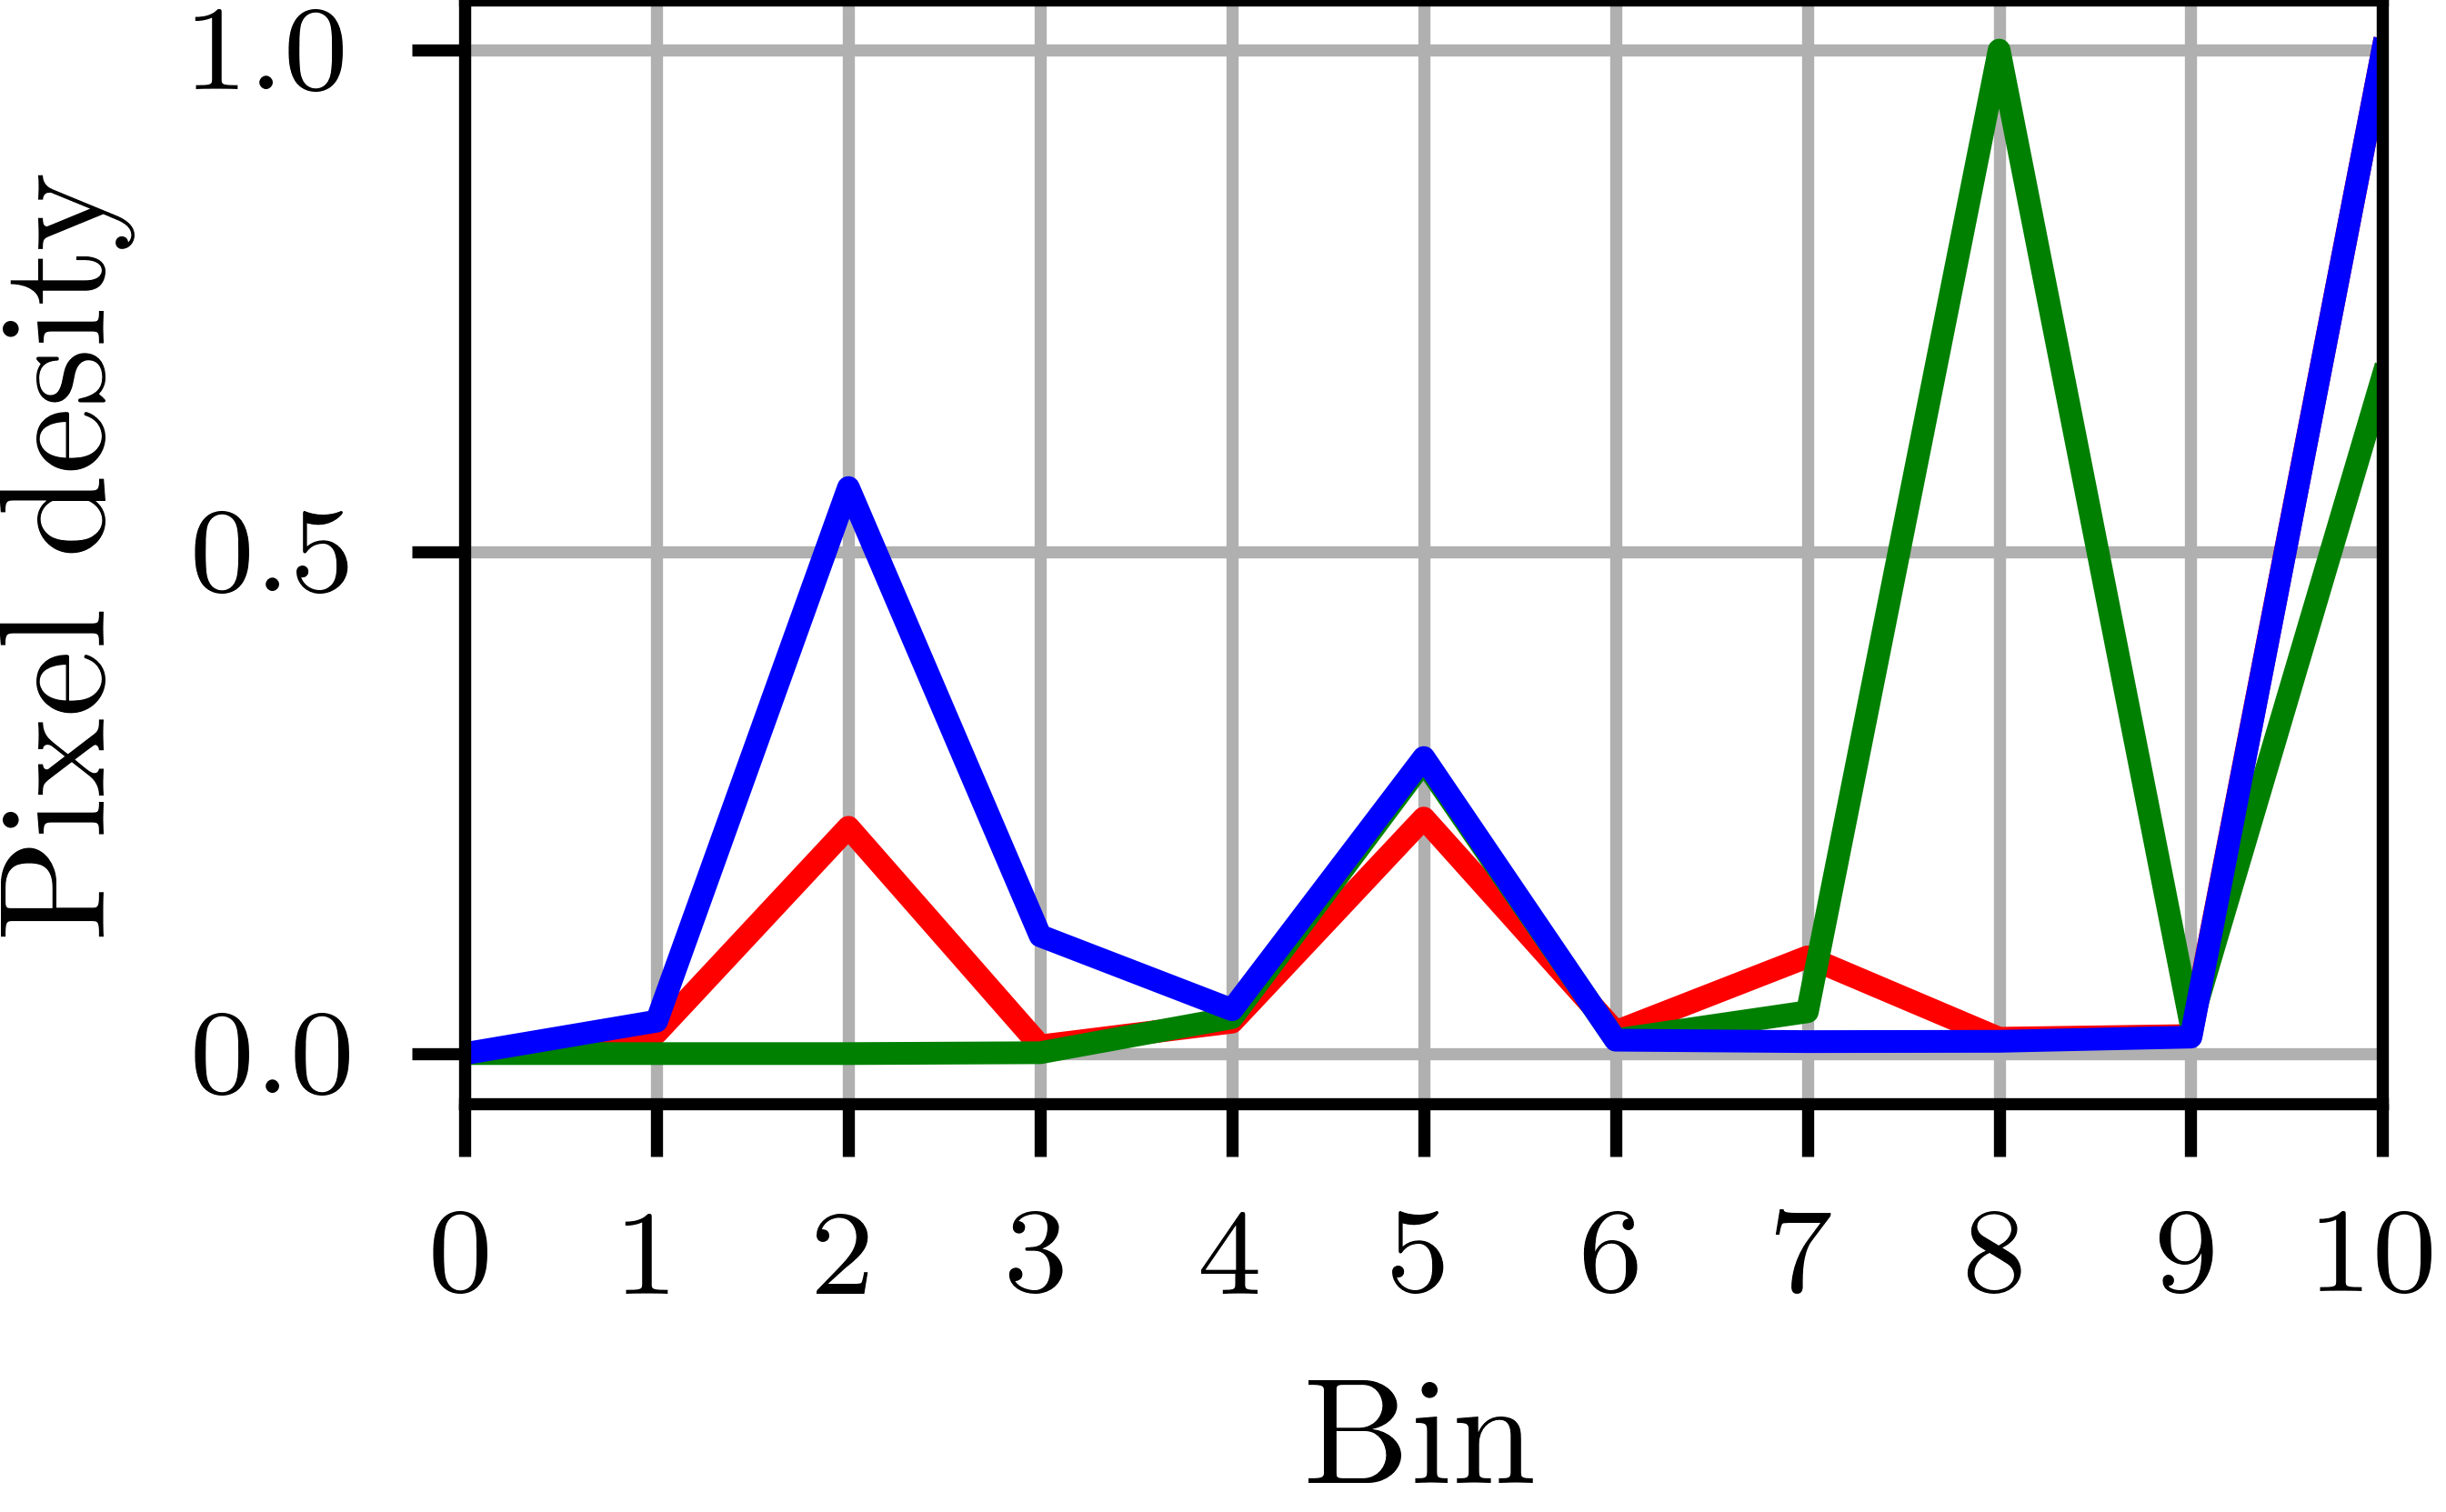
\includegraphics[width=\dimexpr\linewidth-20pt\relax]{tempo_single_histogram}
    \end{subfigure}~     
%    \begin{subfigure}[b]{0.32\textwidth}
%        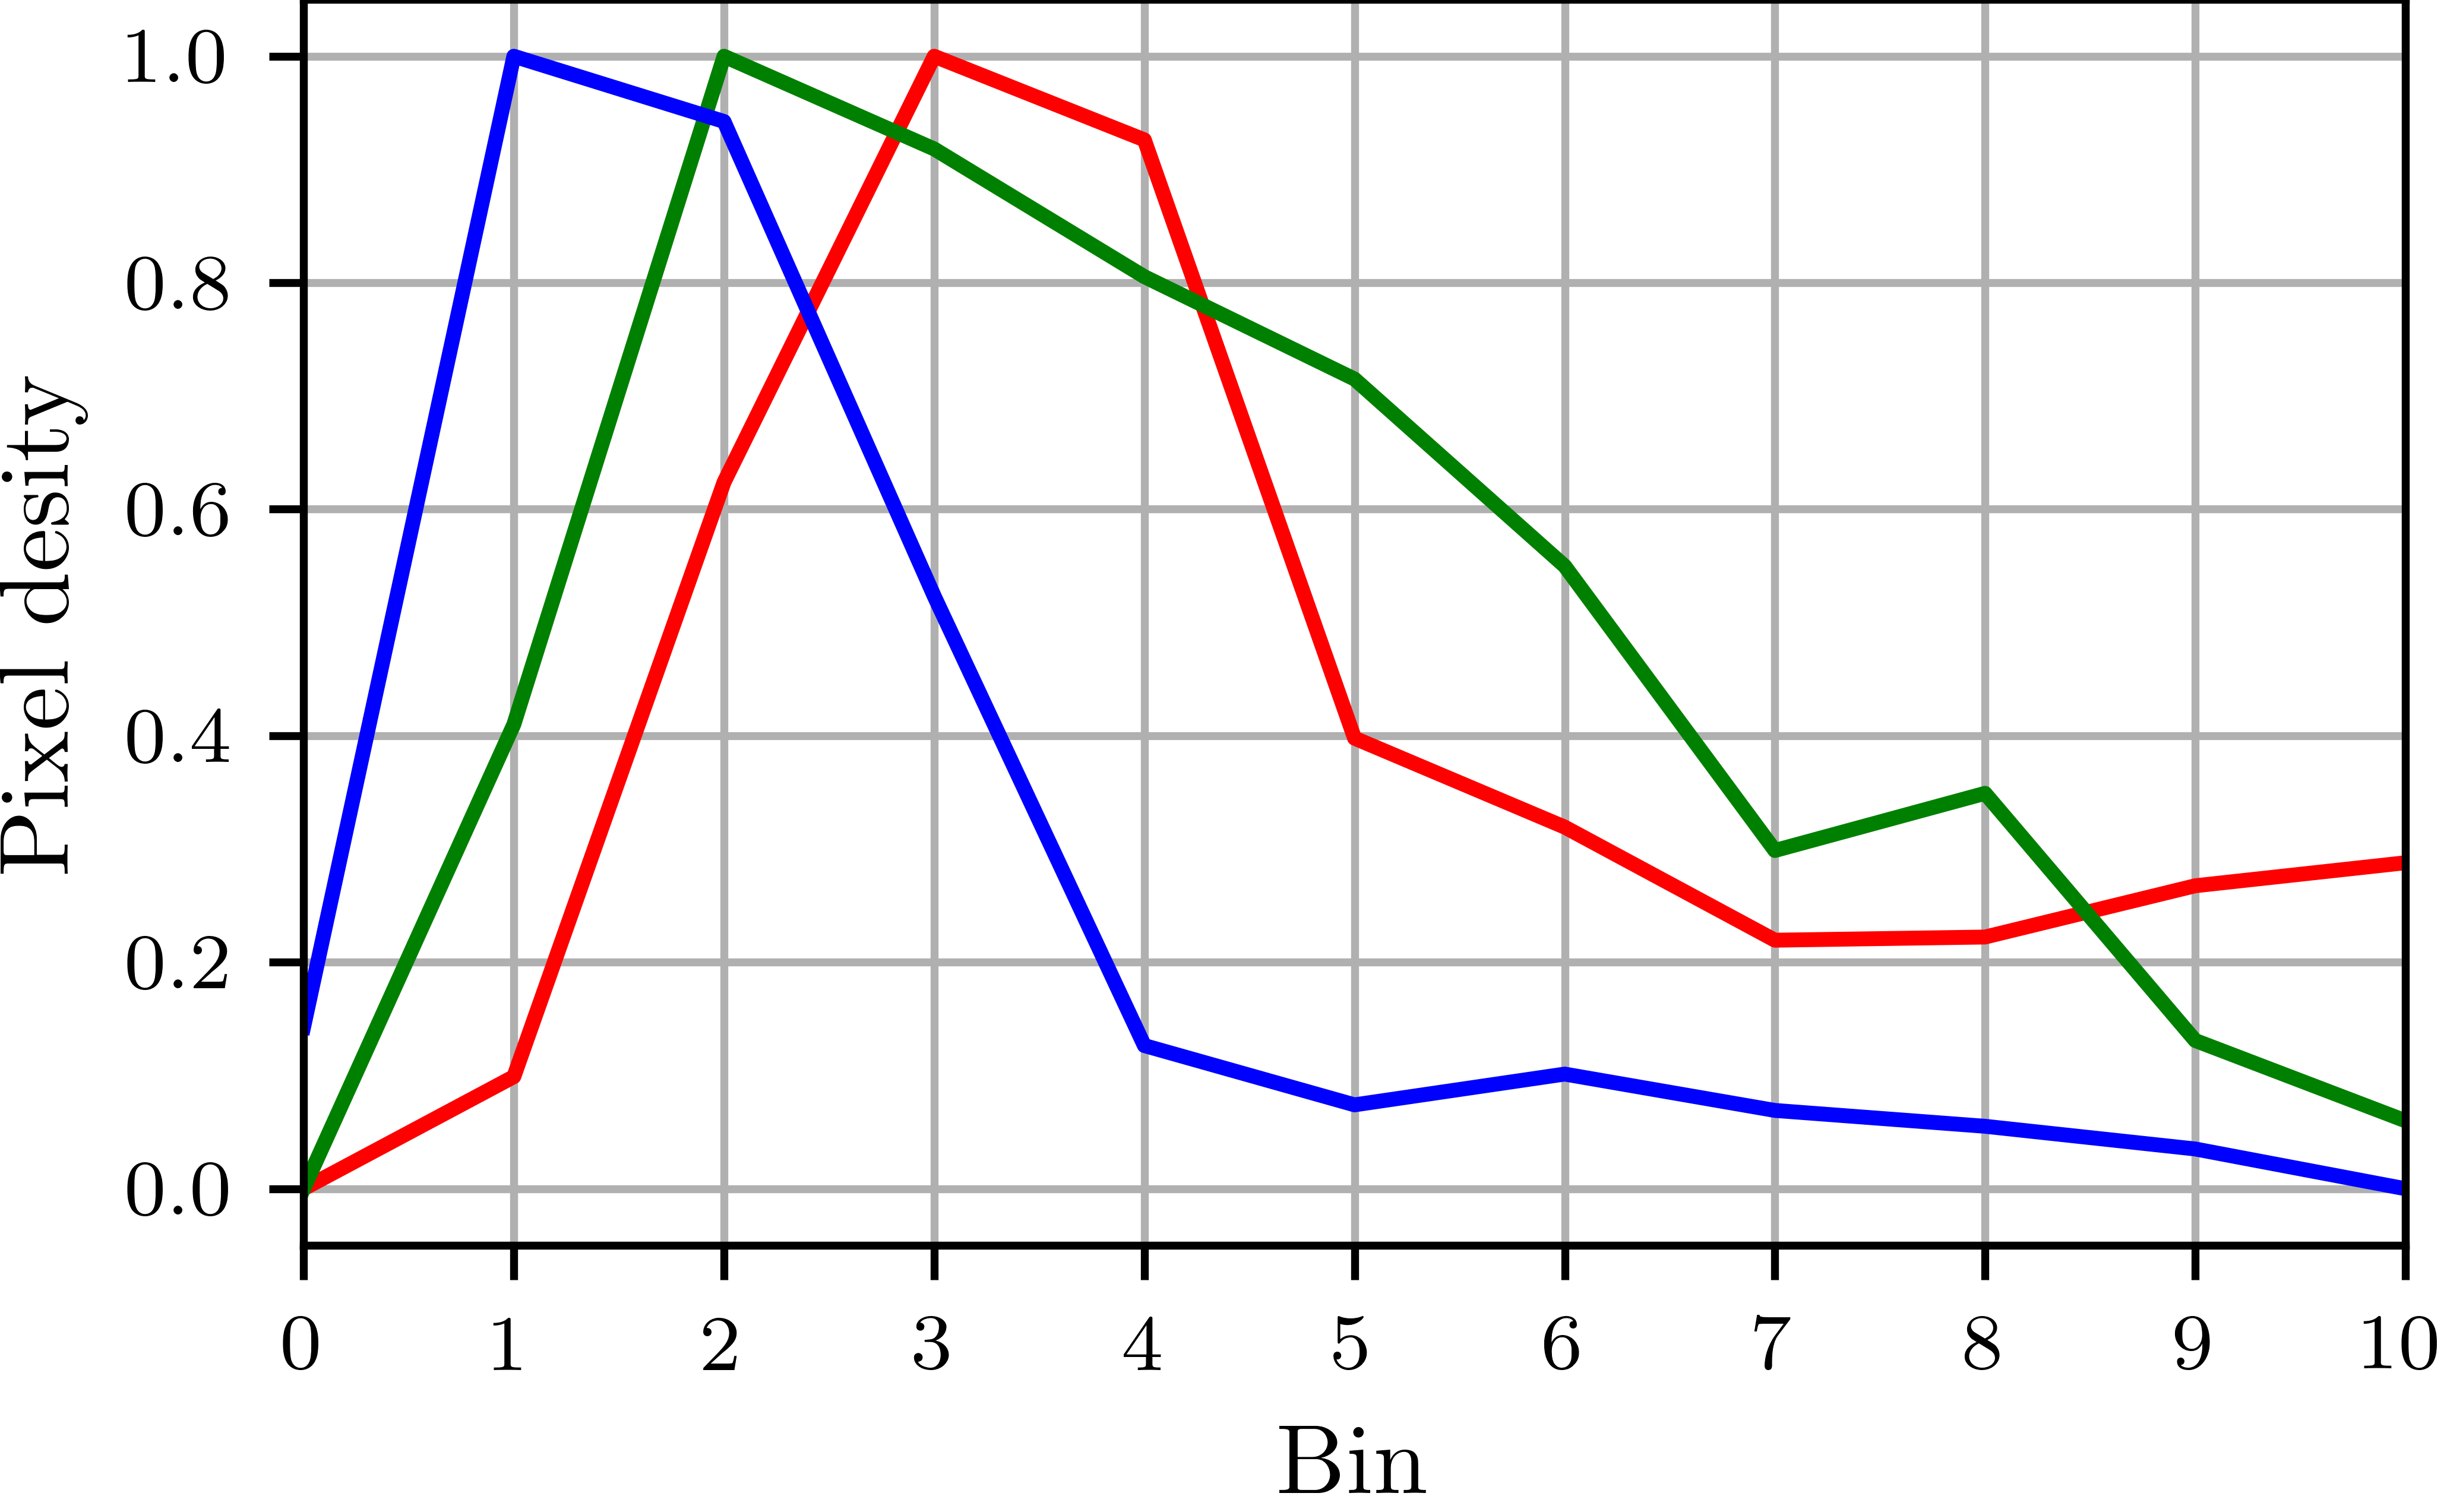
\includegraphics[width=\textwidth]{araras_single_histogram}
%    \end{subfigure}~
    \begin{subfigure}[b]{0.32\textwidth}
        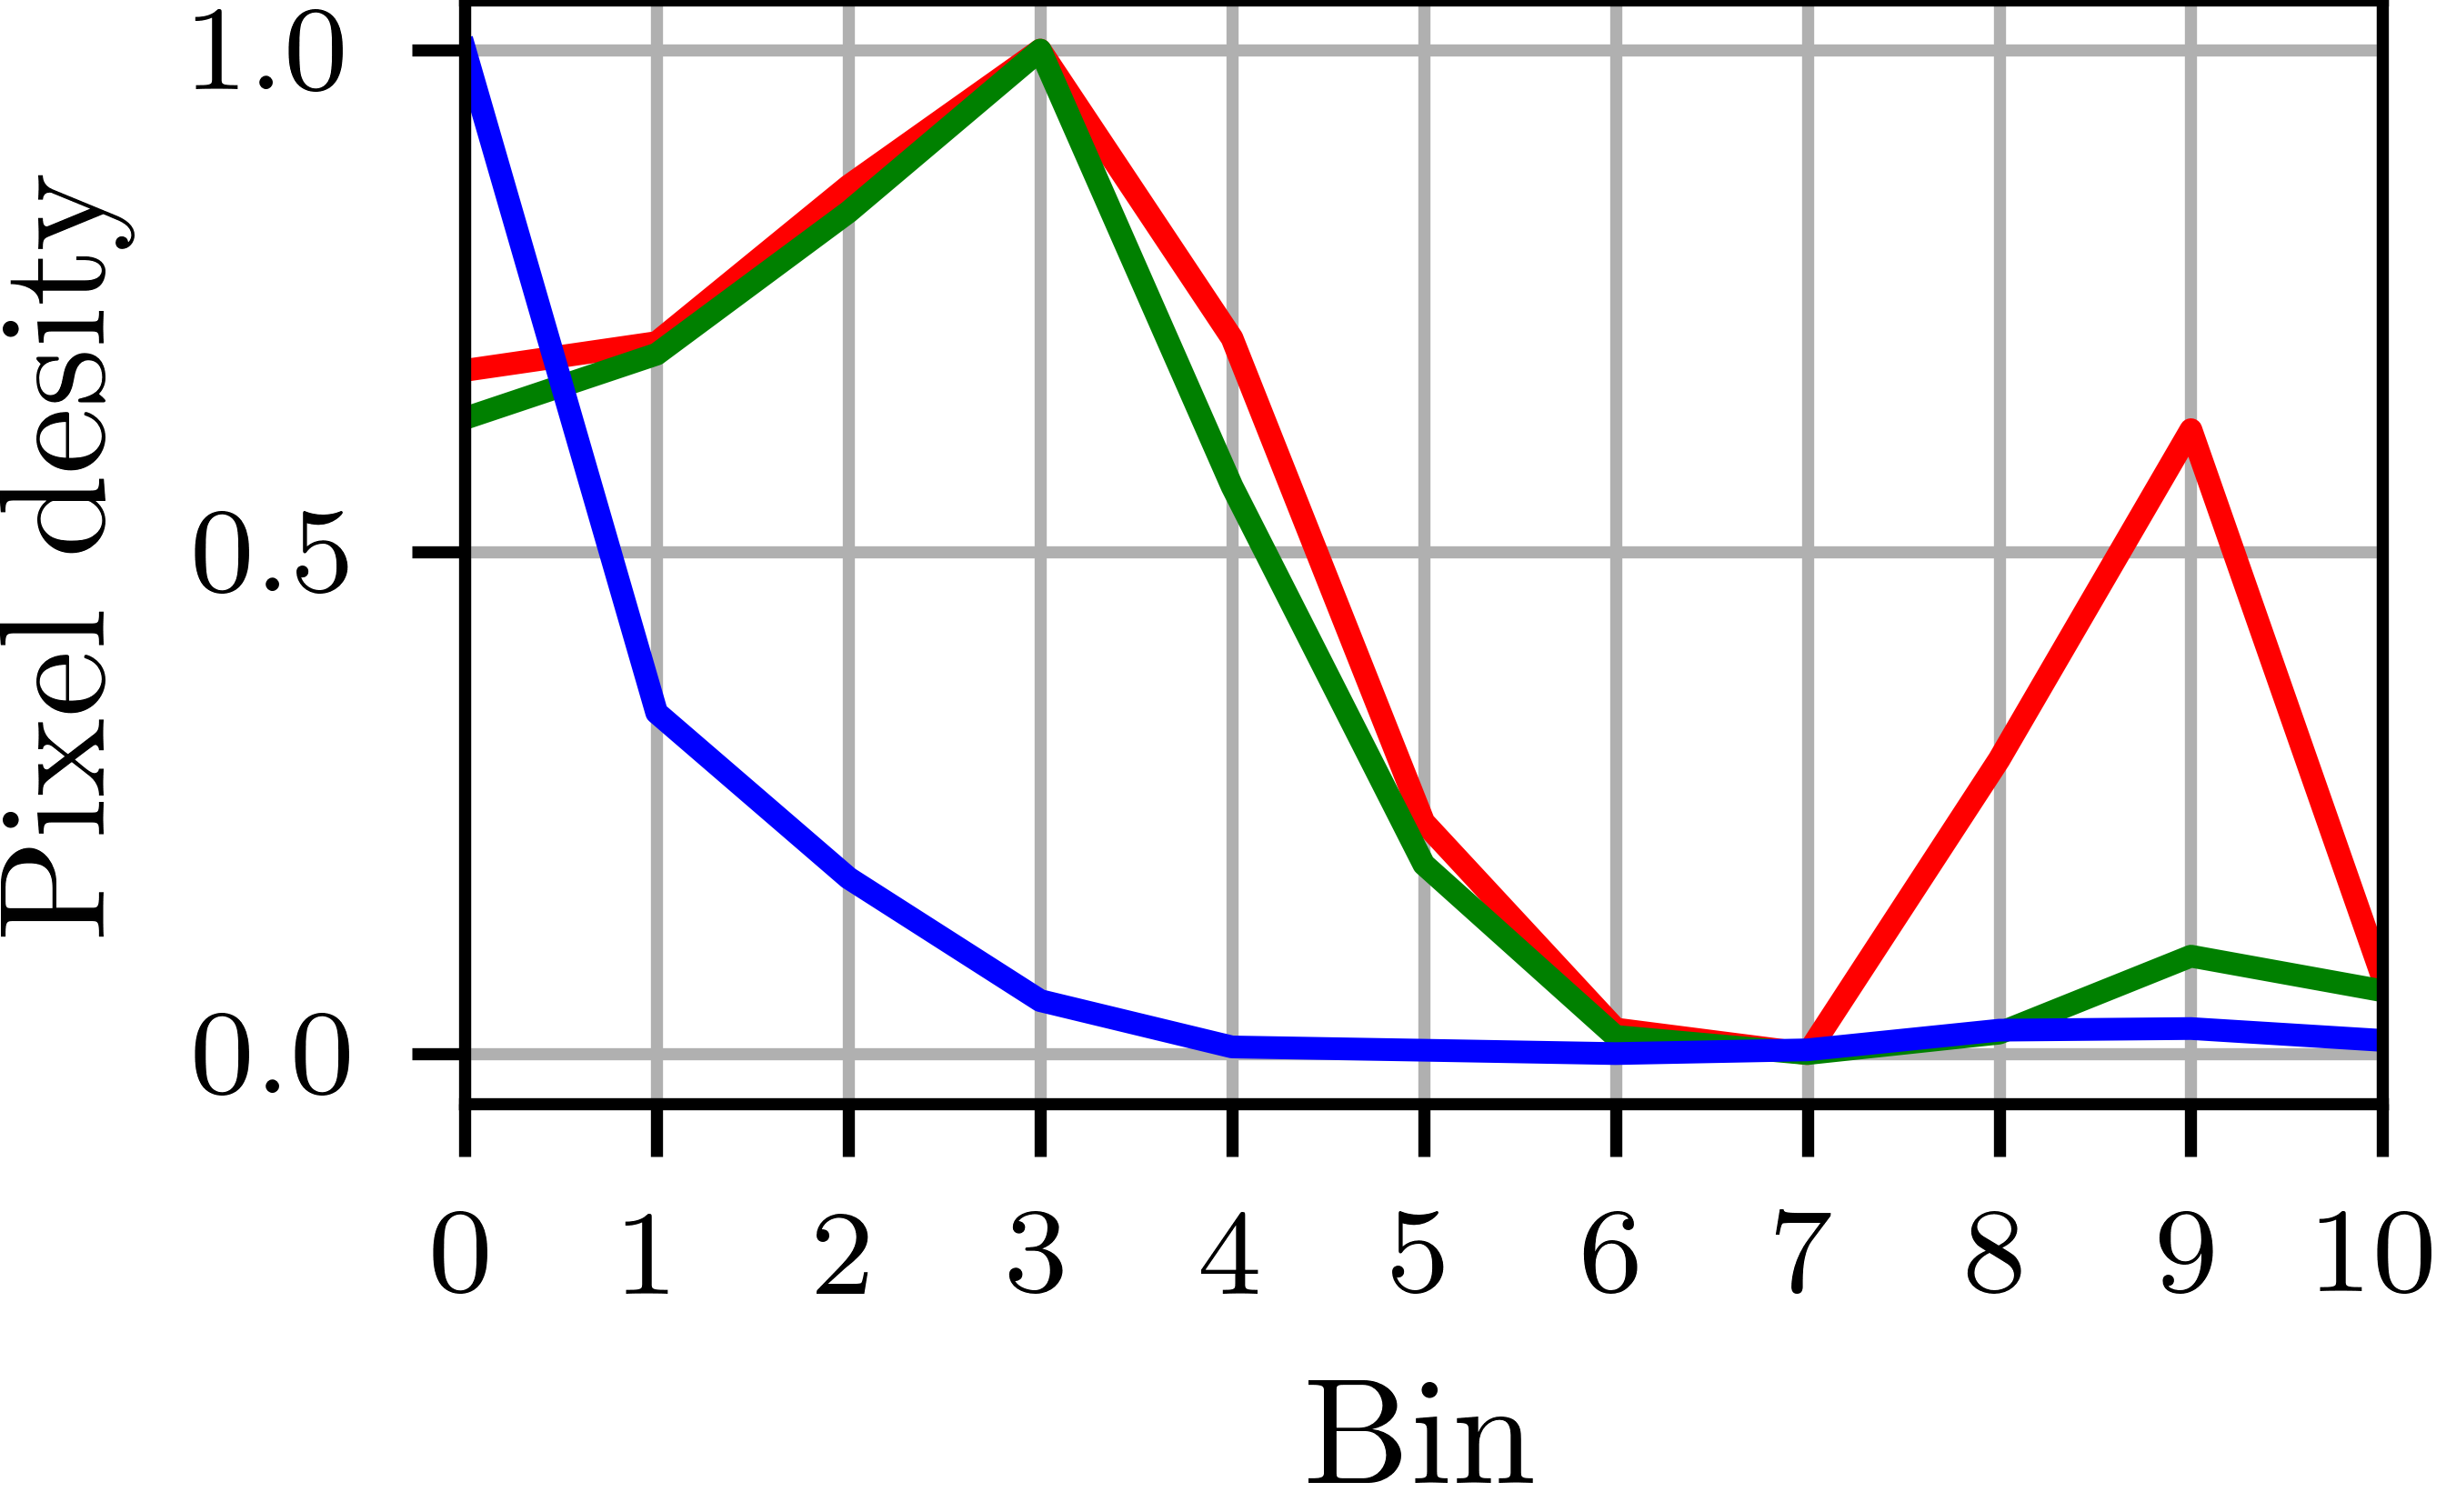
\includegraphics[width=\textwidth]{clownfish_single_histogram}
    \end{subfigure}~
    \begin{subfigure}[b]{0.32\textwidth}
        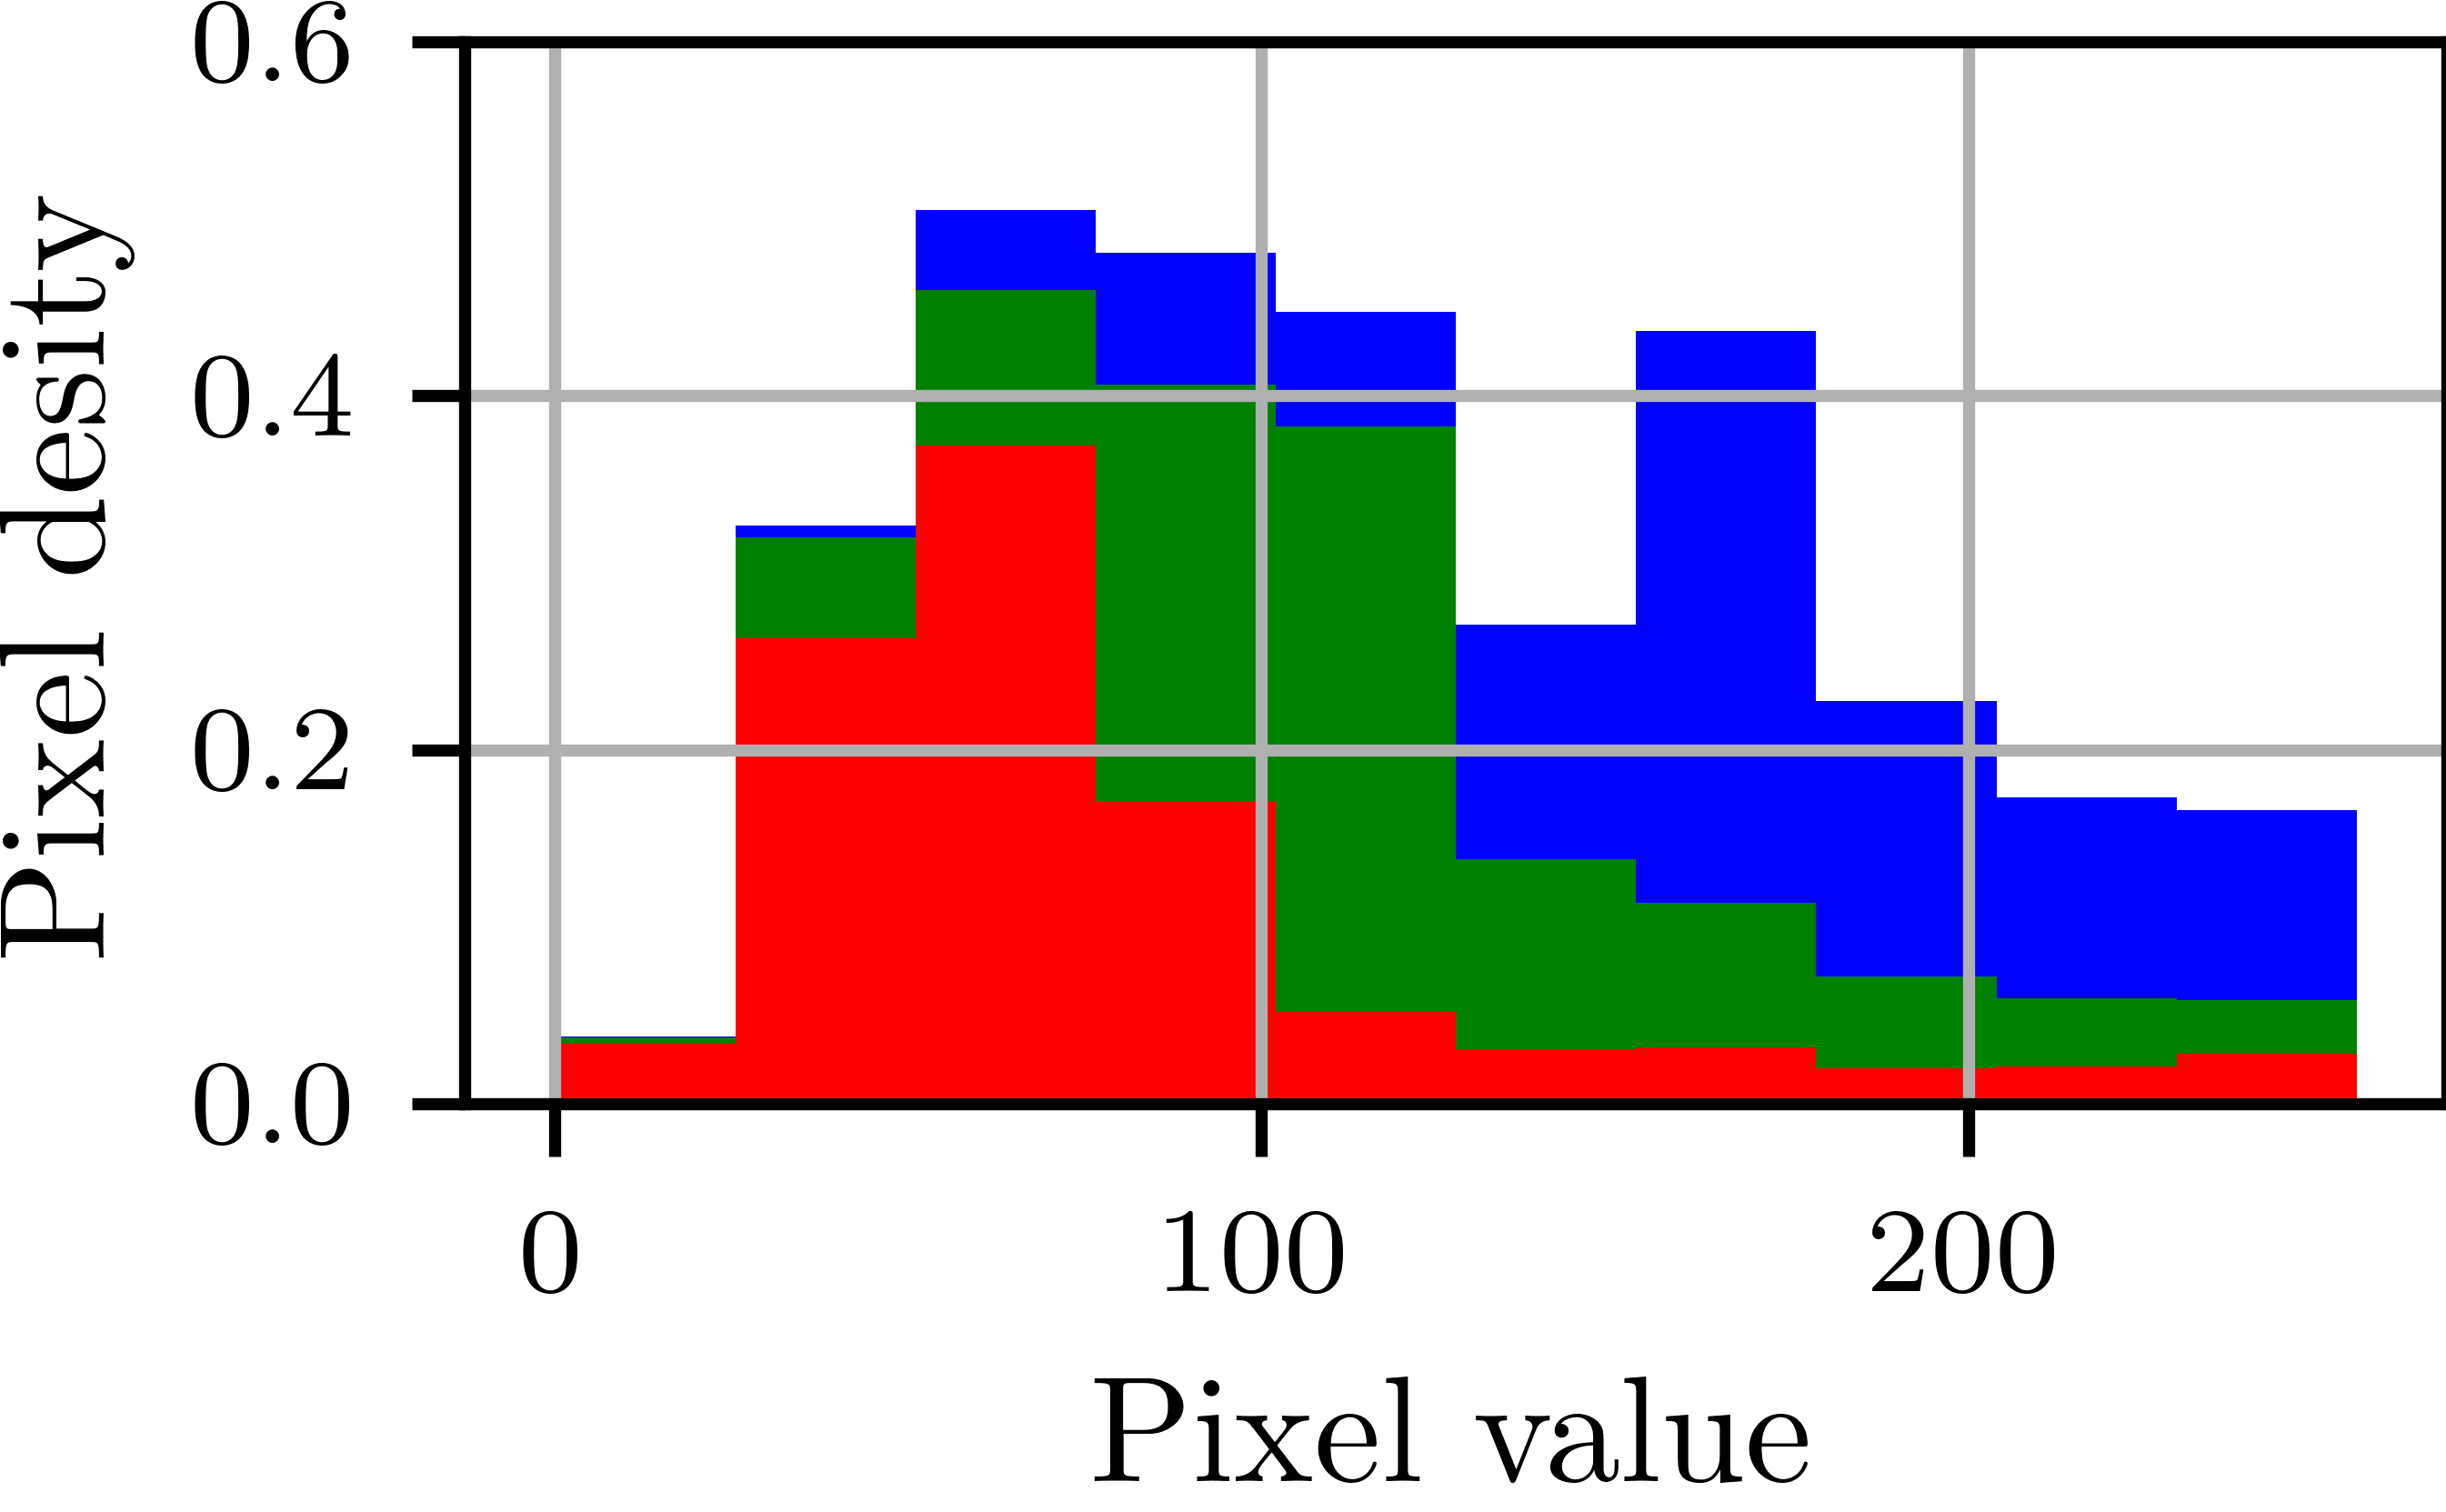
\includegraphics[width=\textwidth]{mountain_single_histogram}
    \end{subfigure}\vspace{10pt}
    
    \begin{subfigure}[t]{\dimexpr0.32\textwidth+20pt\relax}
    	\makebox[20pt]{\raisebox{40pt}{ \small\textbf{\textsf{(c)}} }}%
    	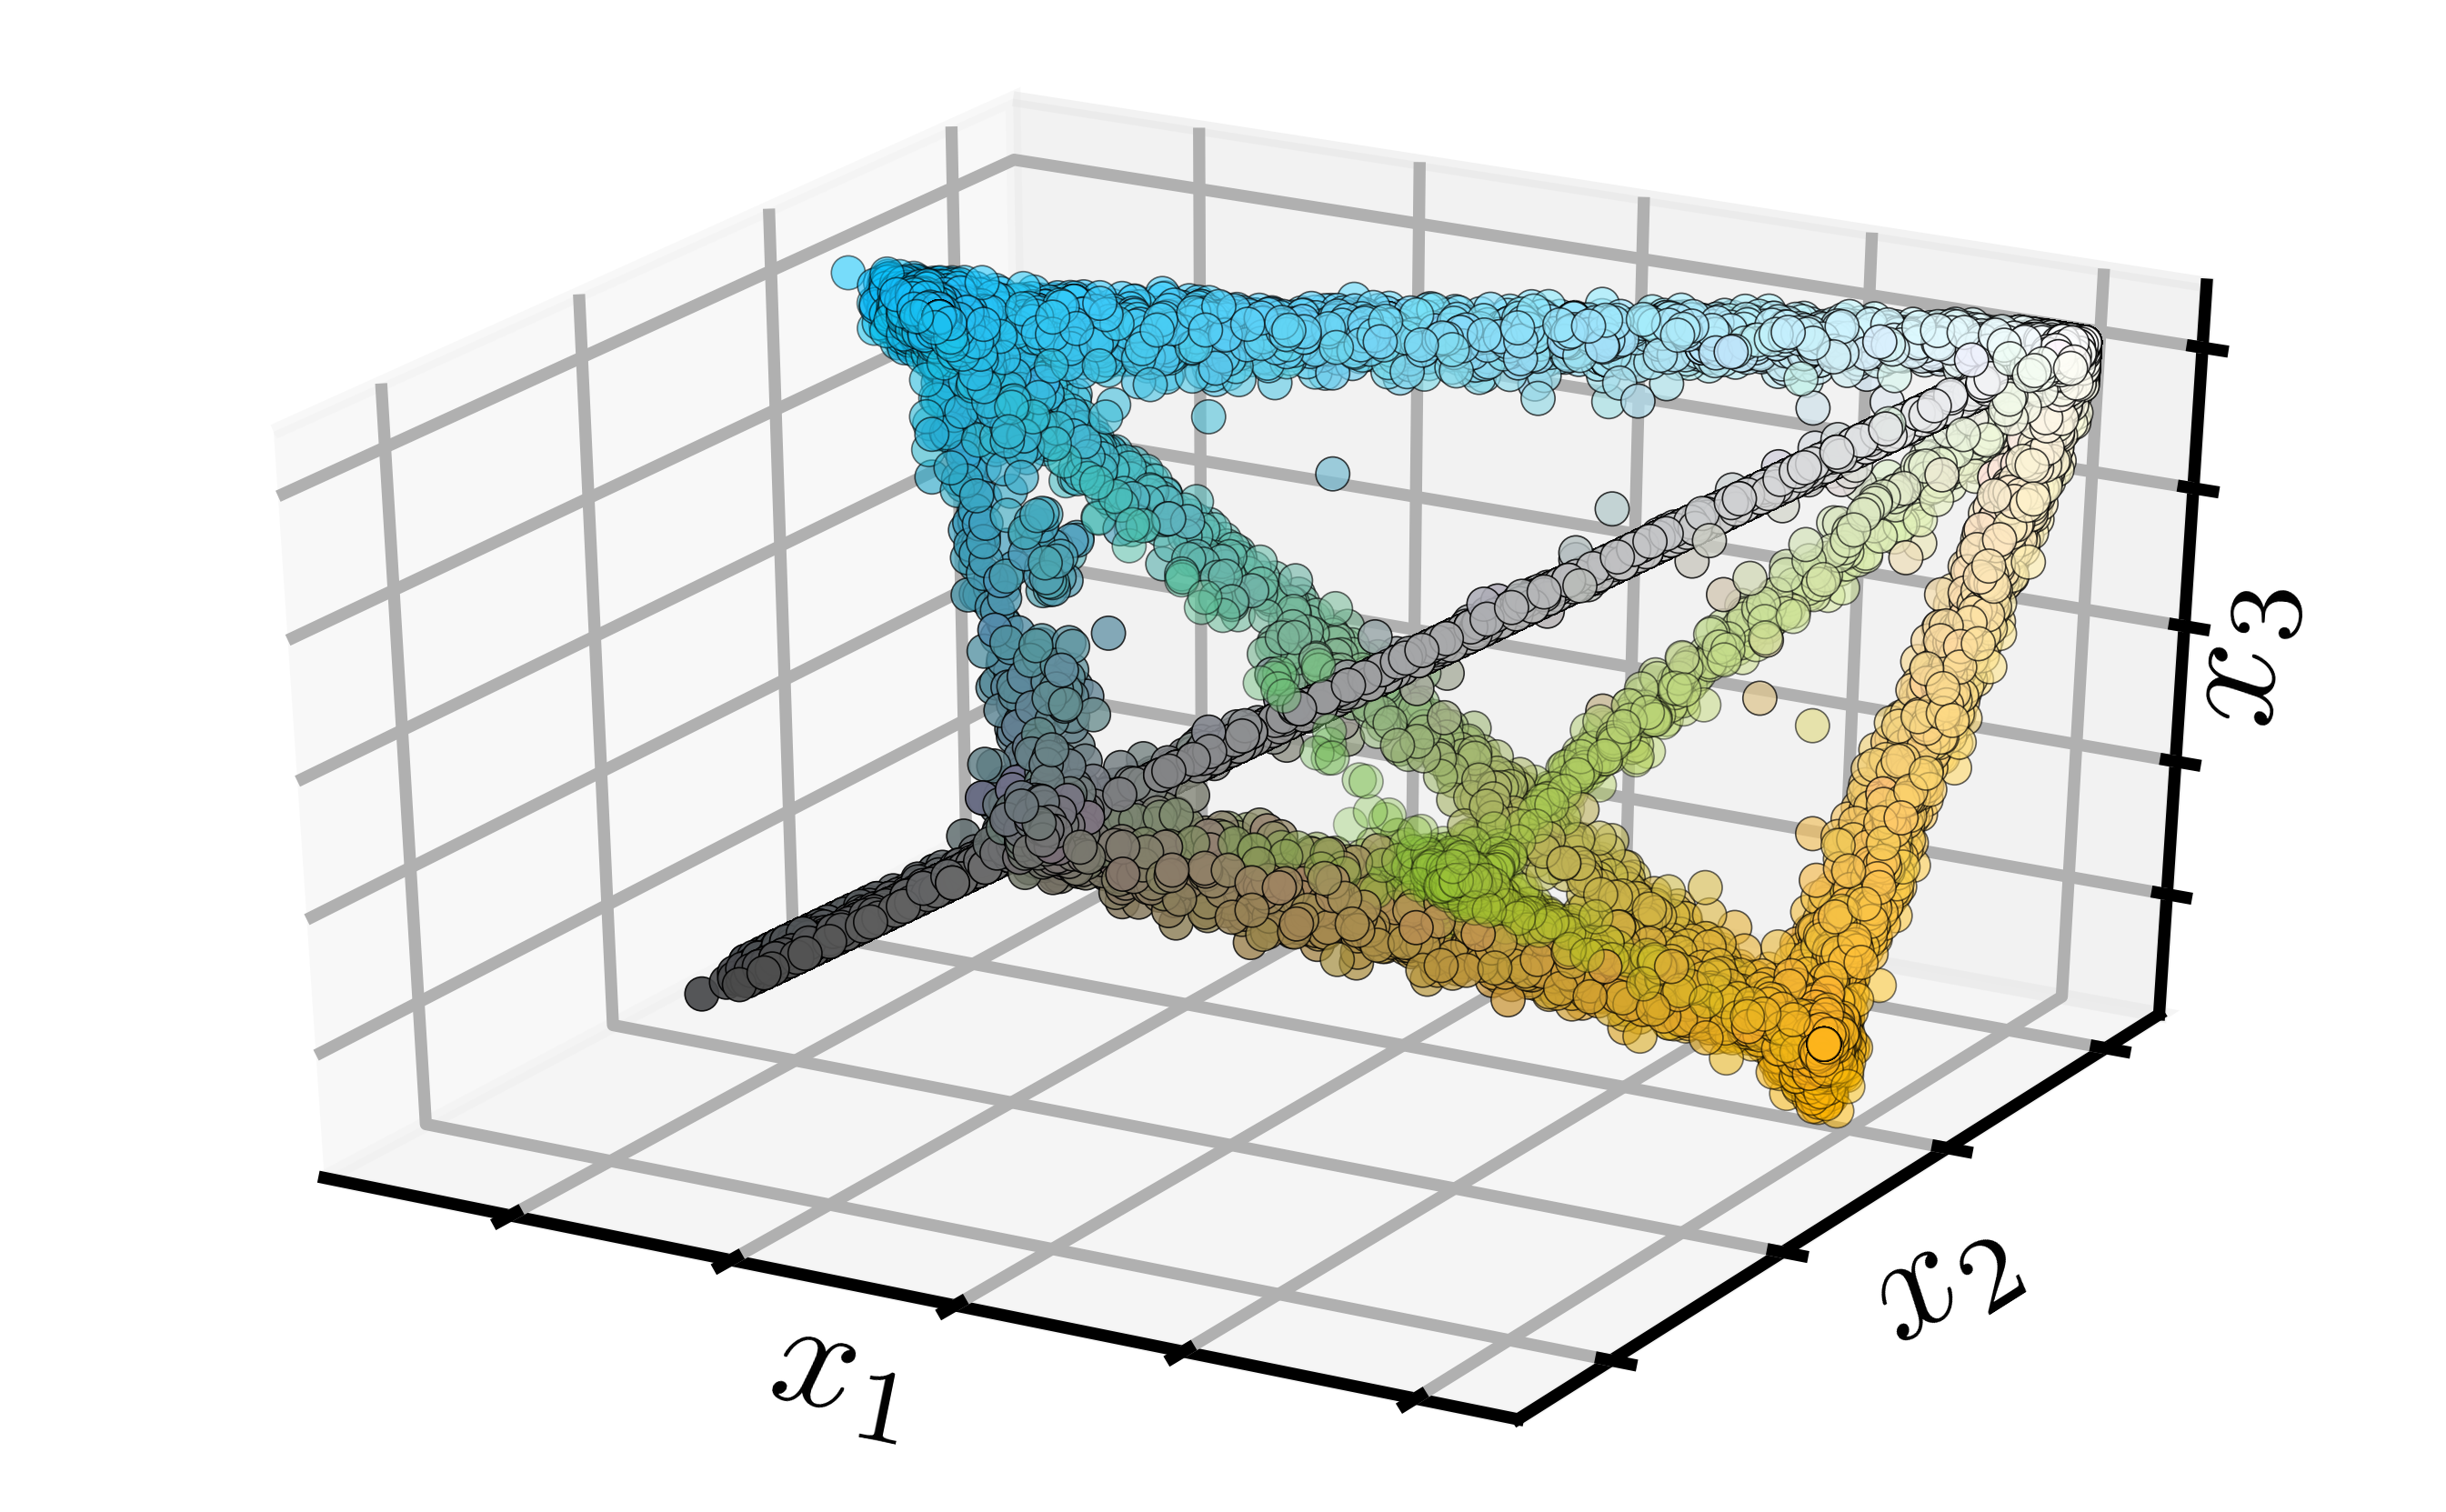
\includegraphics[width=\dimexpr\linewidth-20pt\relax]{tempo_3d_distribution}
    \end{subfigure}~ 
%    \begin{subfigure}[b]{0.32\textwidth}
%        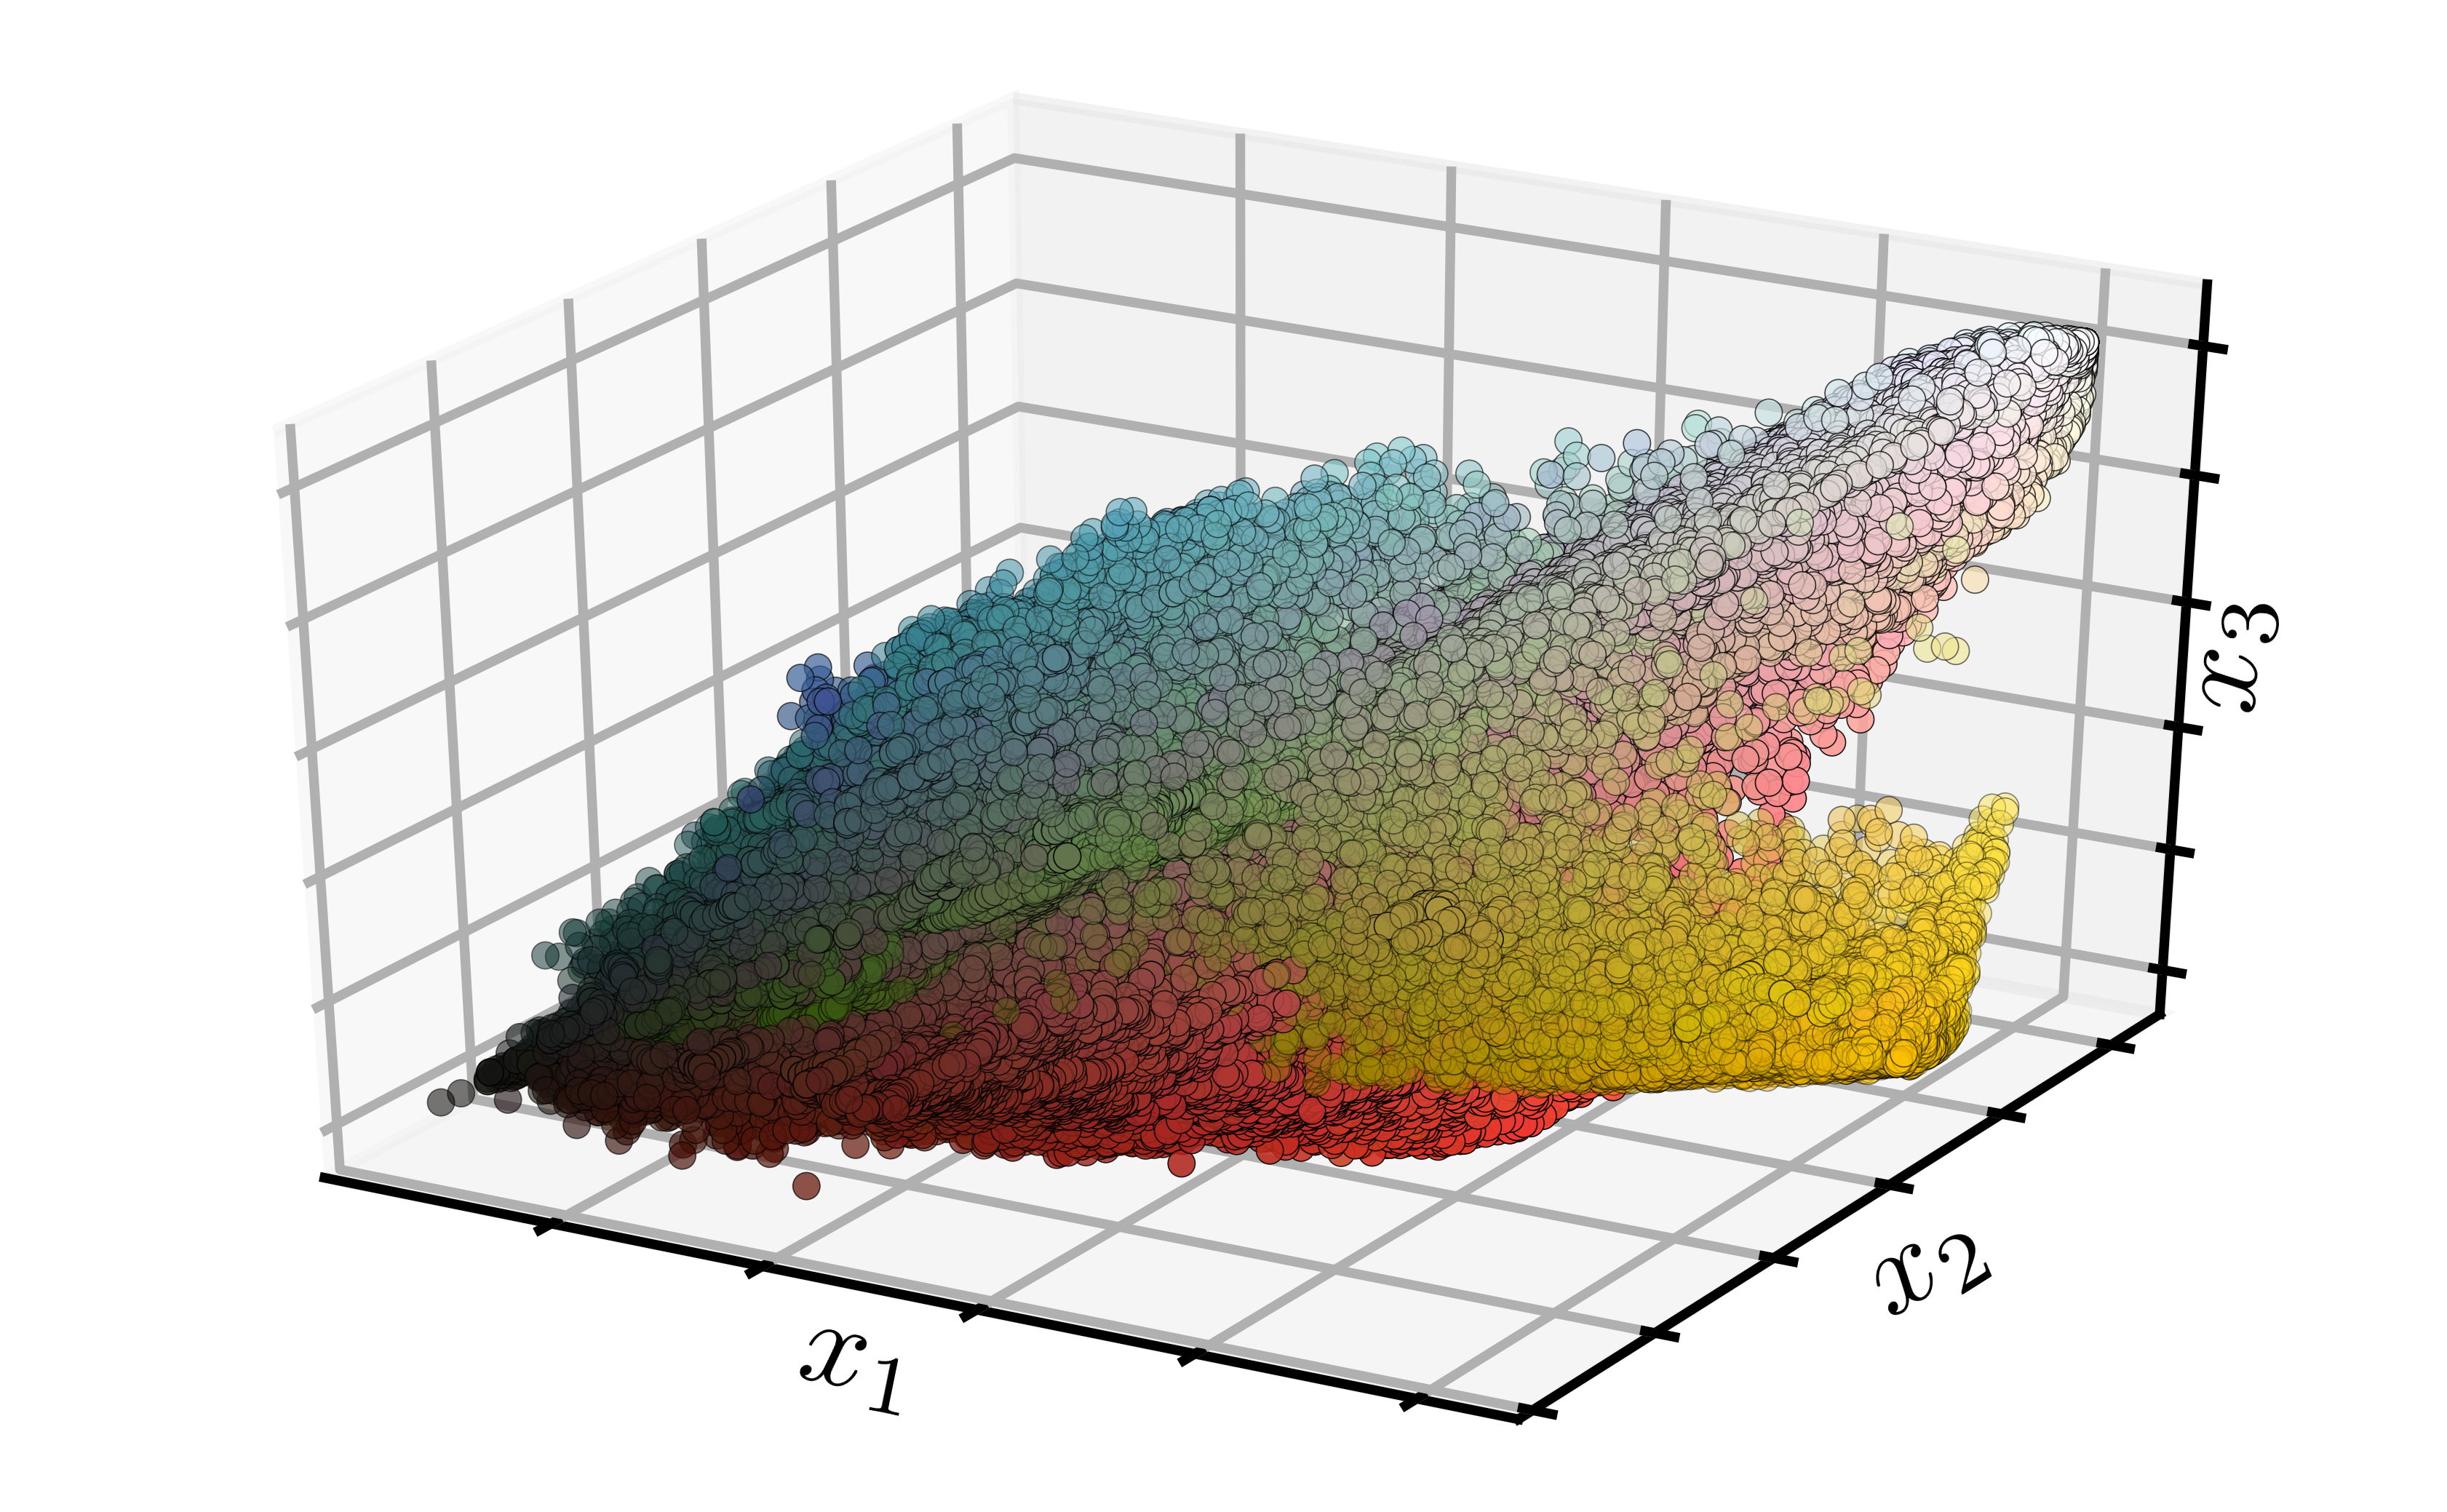
\includegraphics[width=\textwidth]{araras_3d_distribution}
%    \end{subfigure}~
    \begin{subfigure}[b]{0.32\textwidth}
        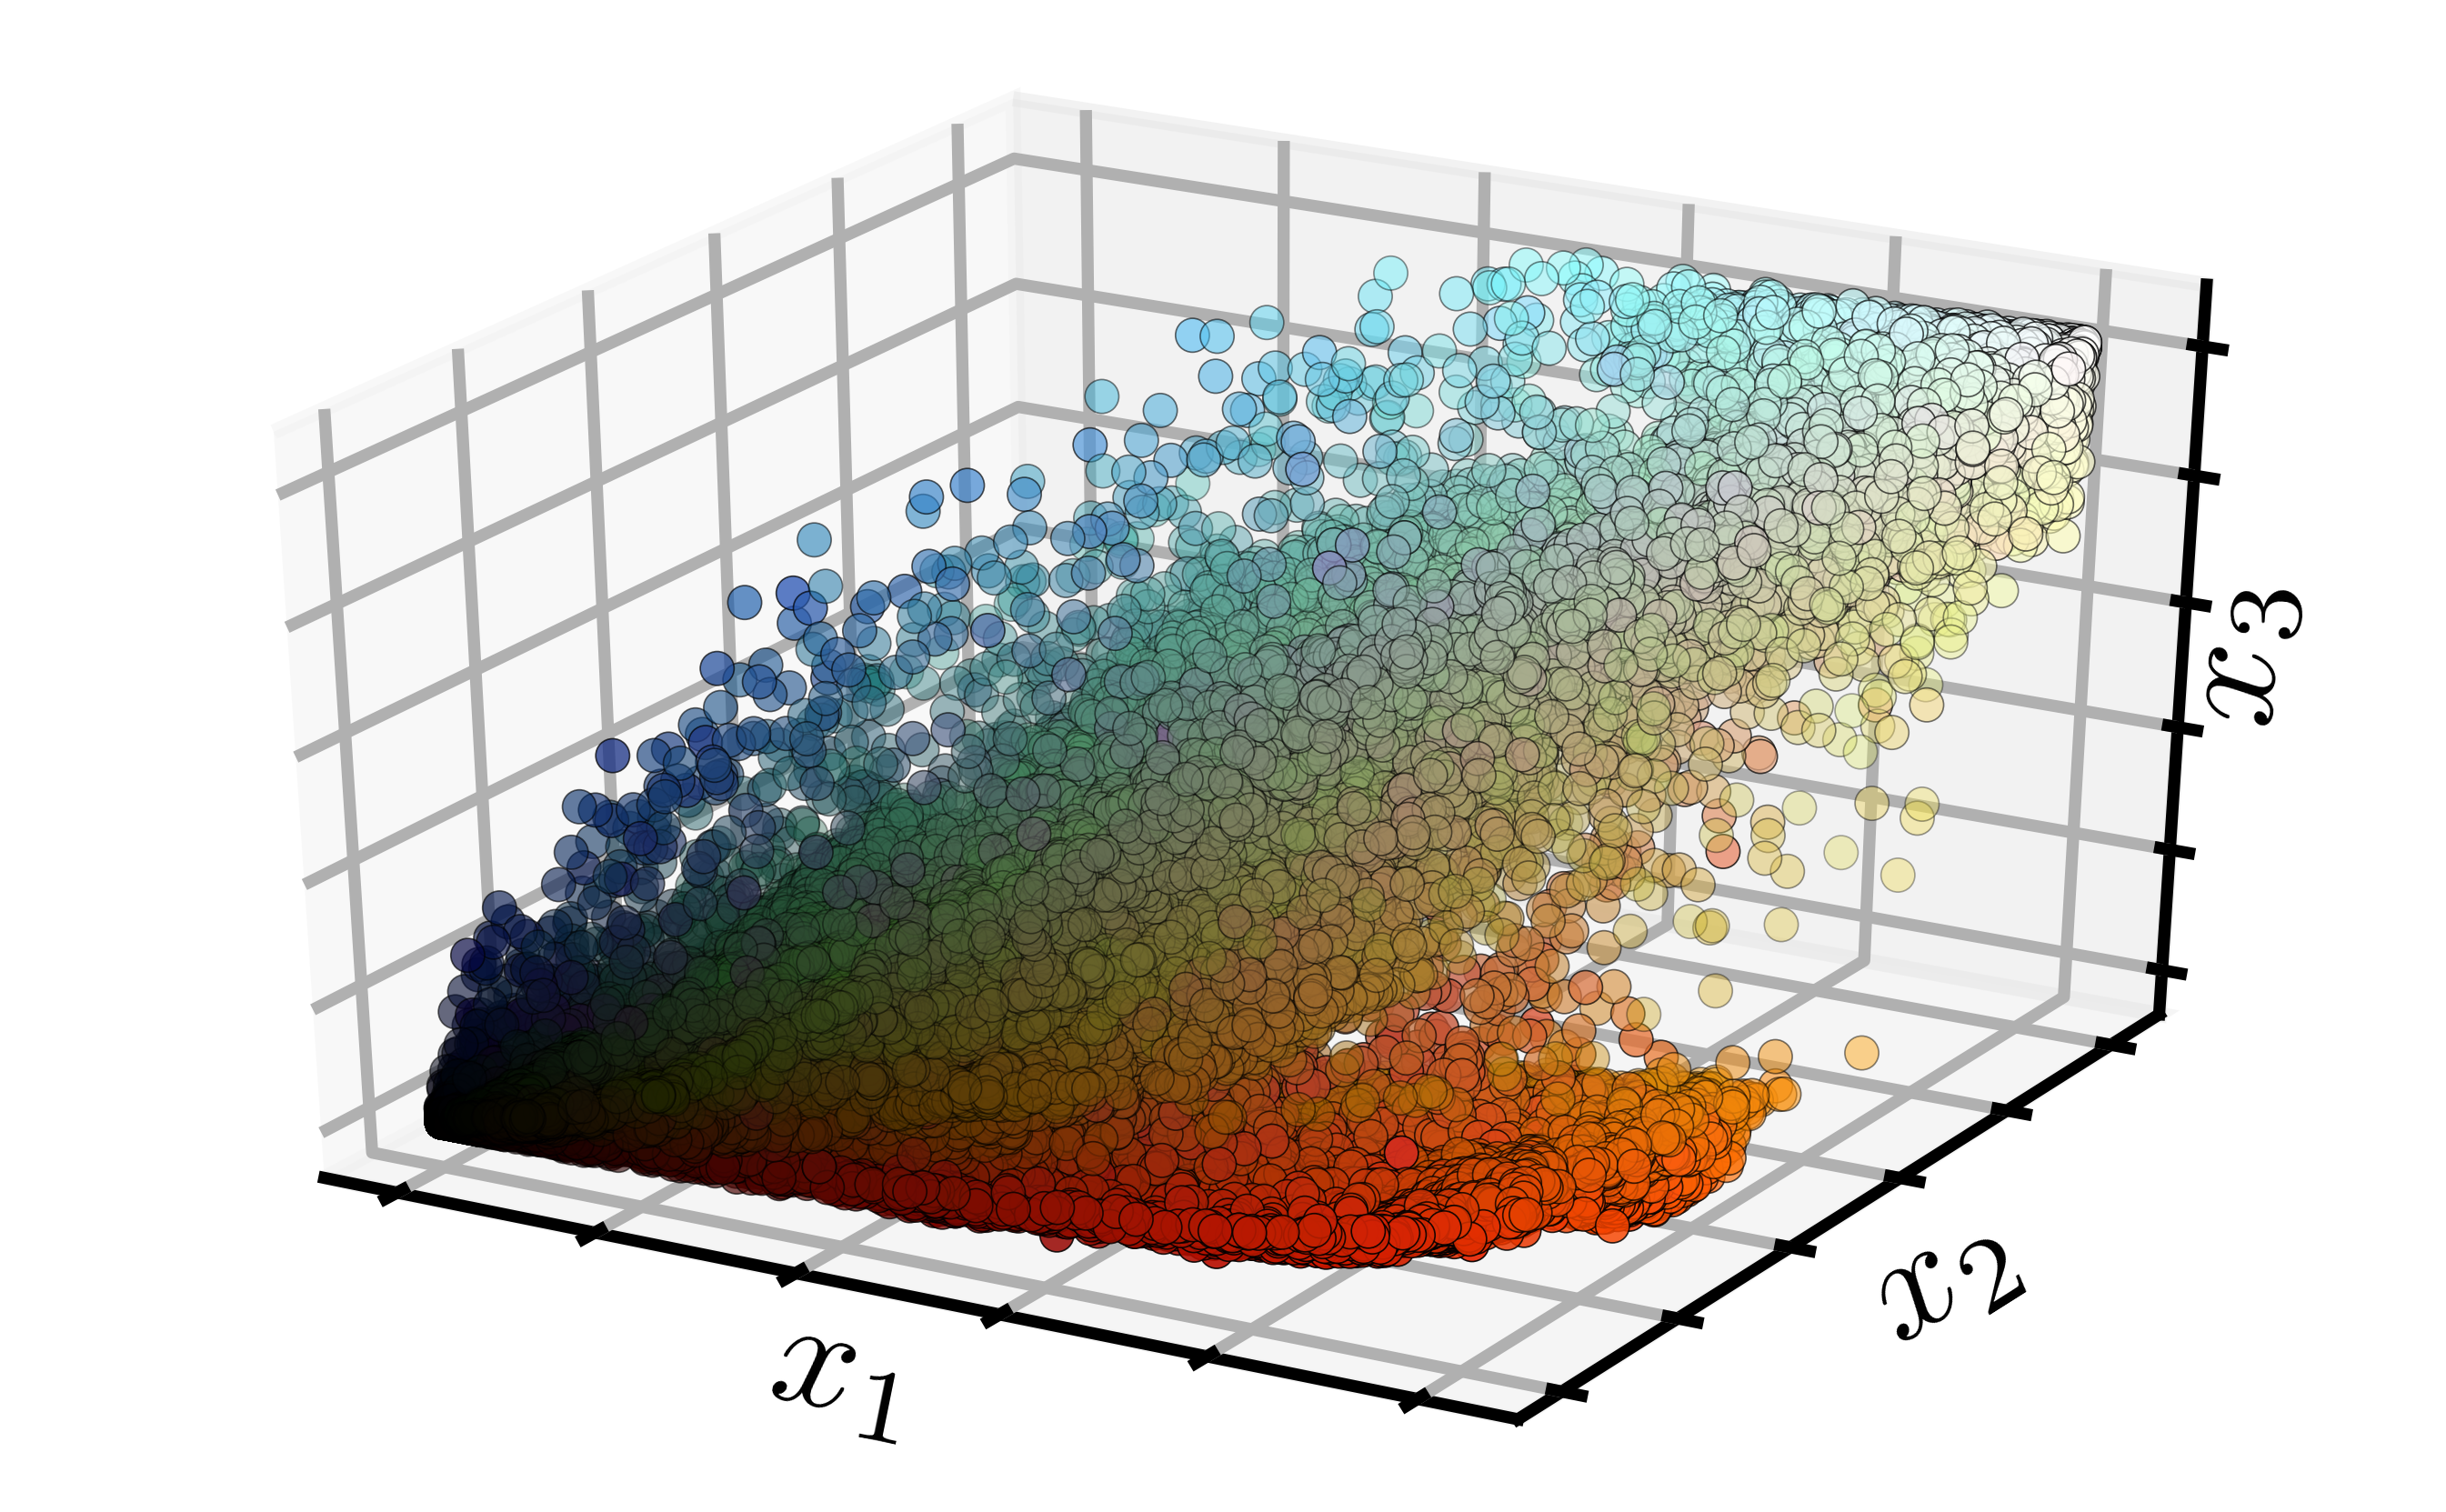
\includegraphics[width=\textwidth]{clownfish_3d_distribution}
    \end{subfigure}~
    \begin{subfigure}[b]{0.32\textwidth}
        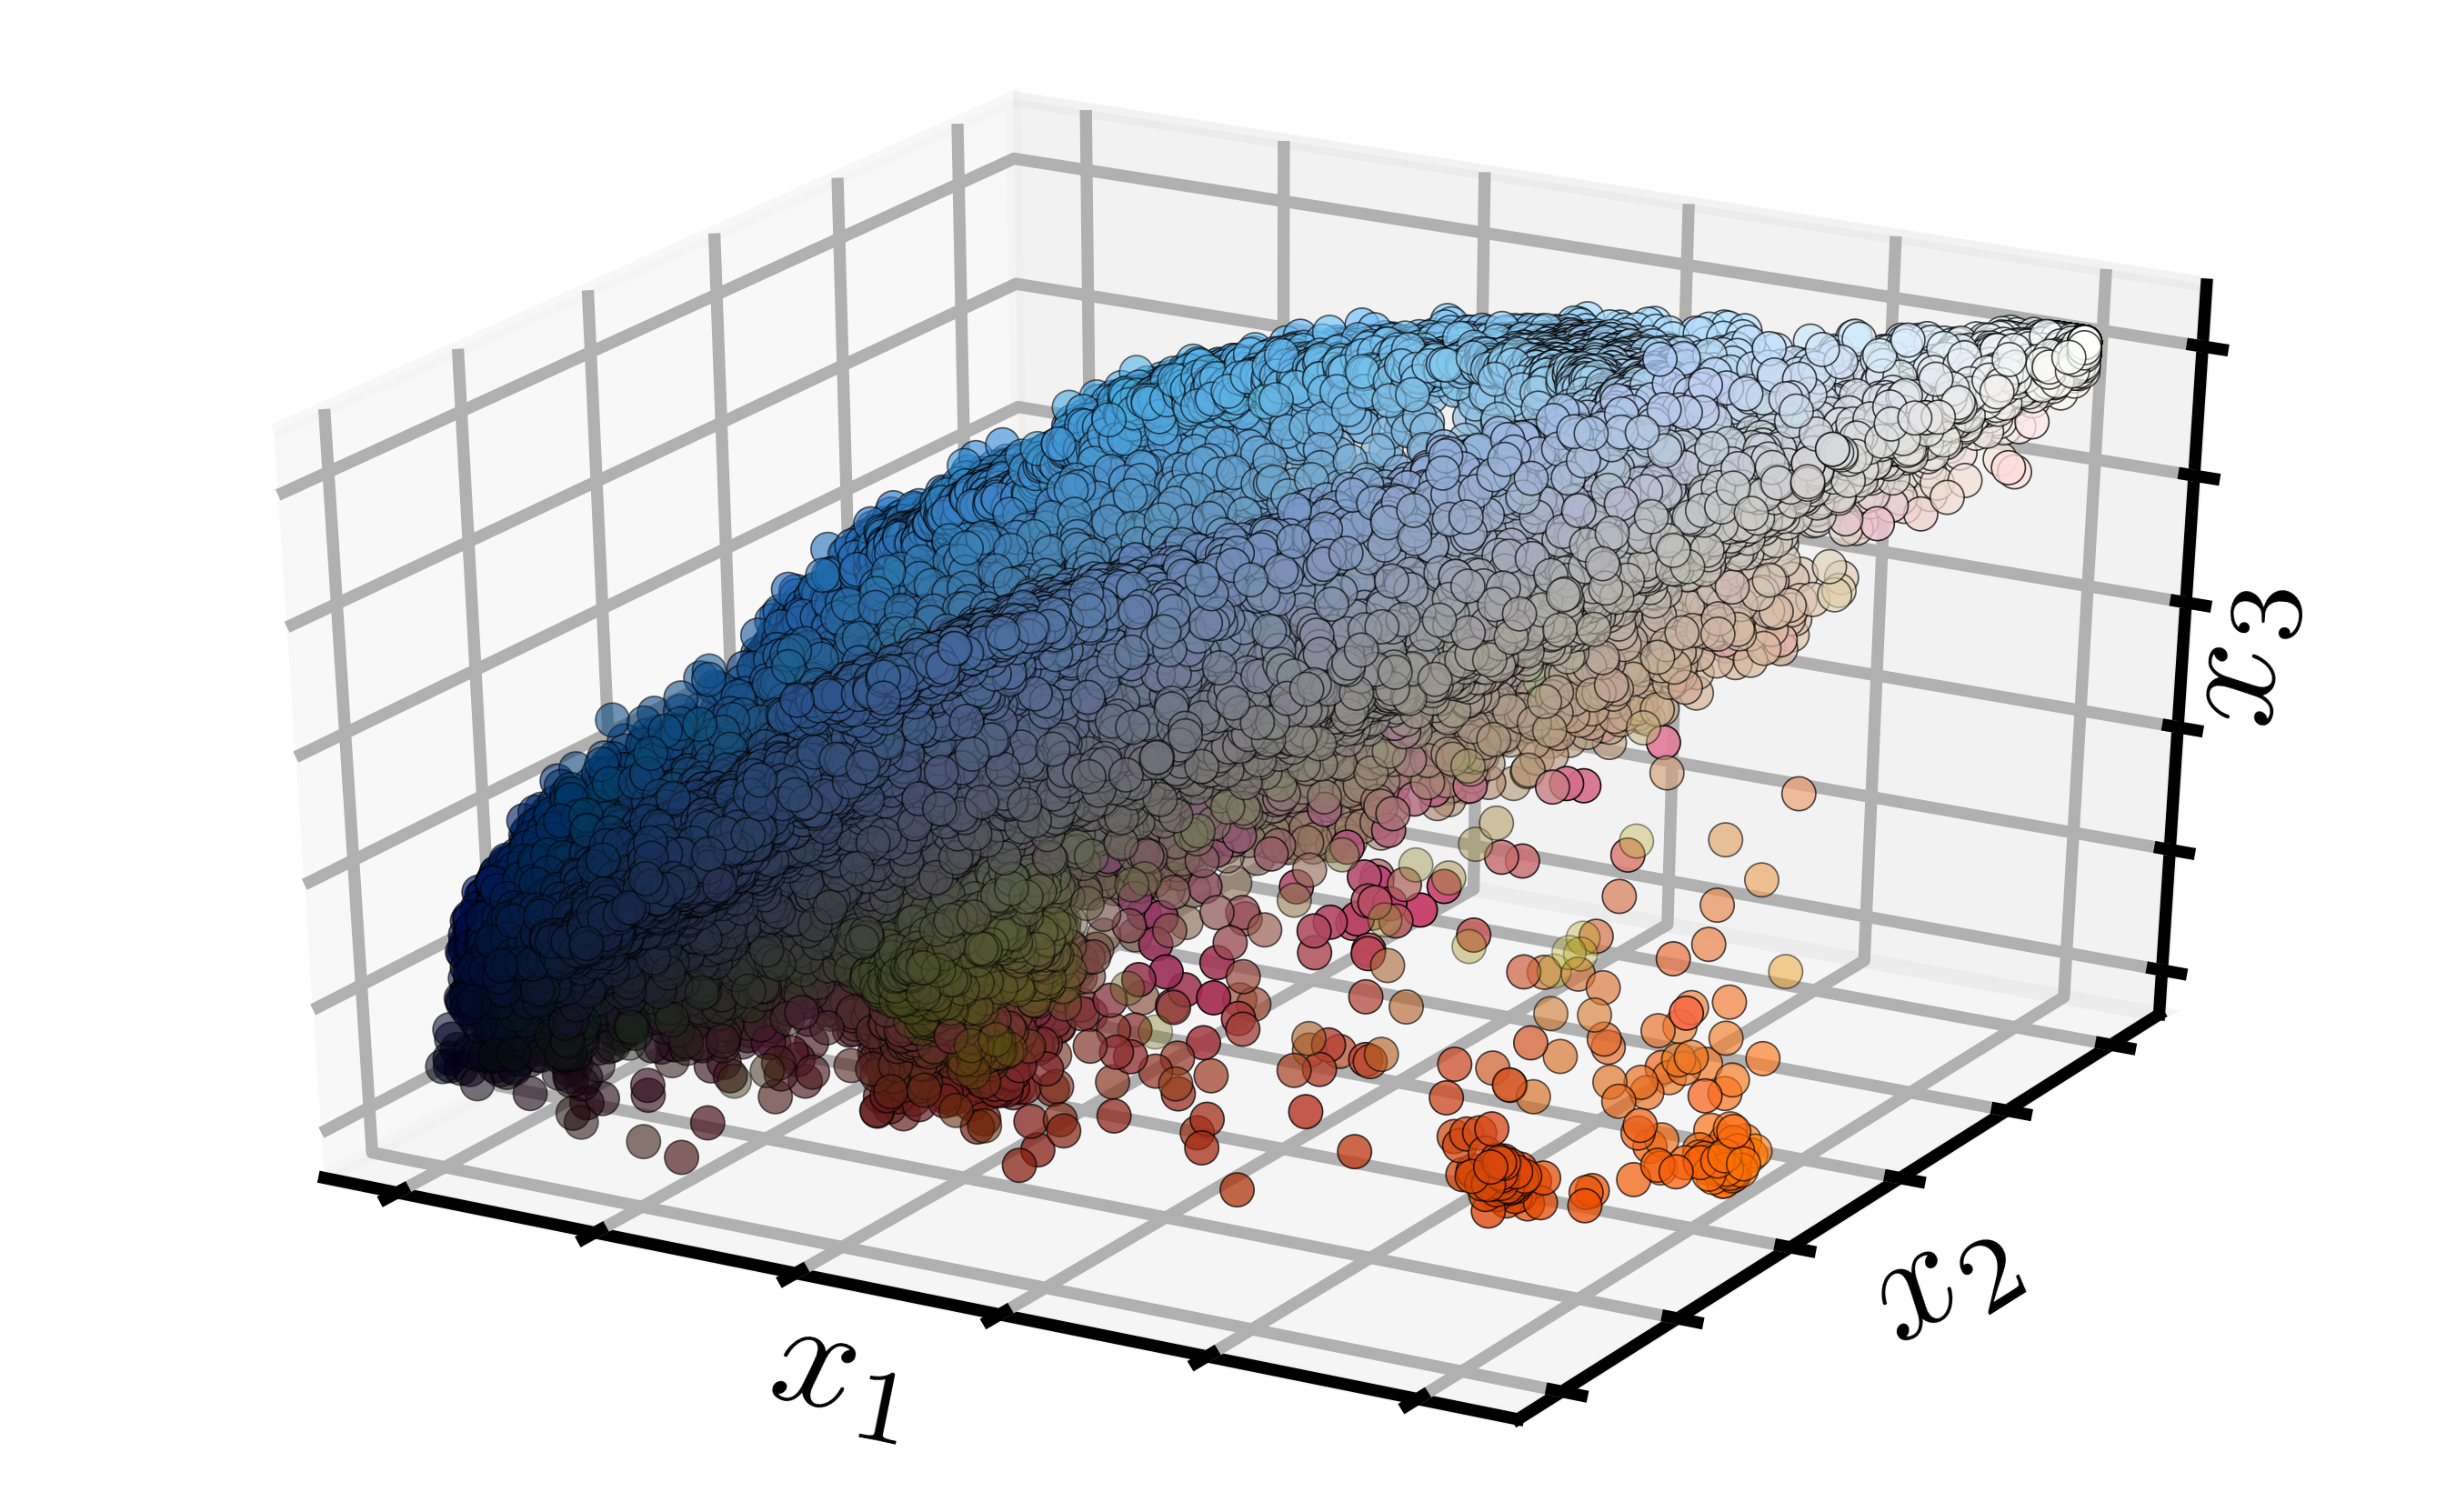
\includegraphics[width=\textwidth]{mountain_3d_distribution}
    \end{subfigure}\vspace{10pt}
    
    \begin{subfigure}[t]{\dimexpr0.32\textwidth+20pt\relax}
    	\makebox[20pt]{\raisebox{40pt}{ \small\textbf{\textsf{(d)}} }}%
    	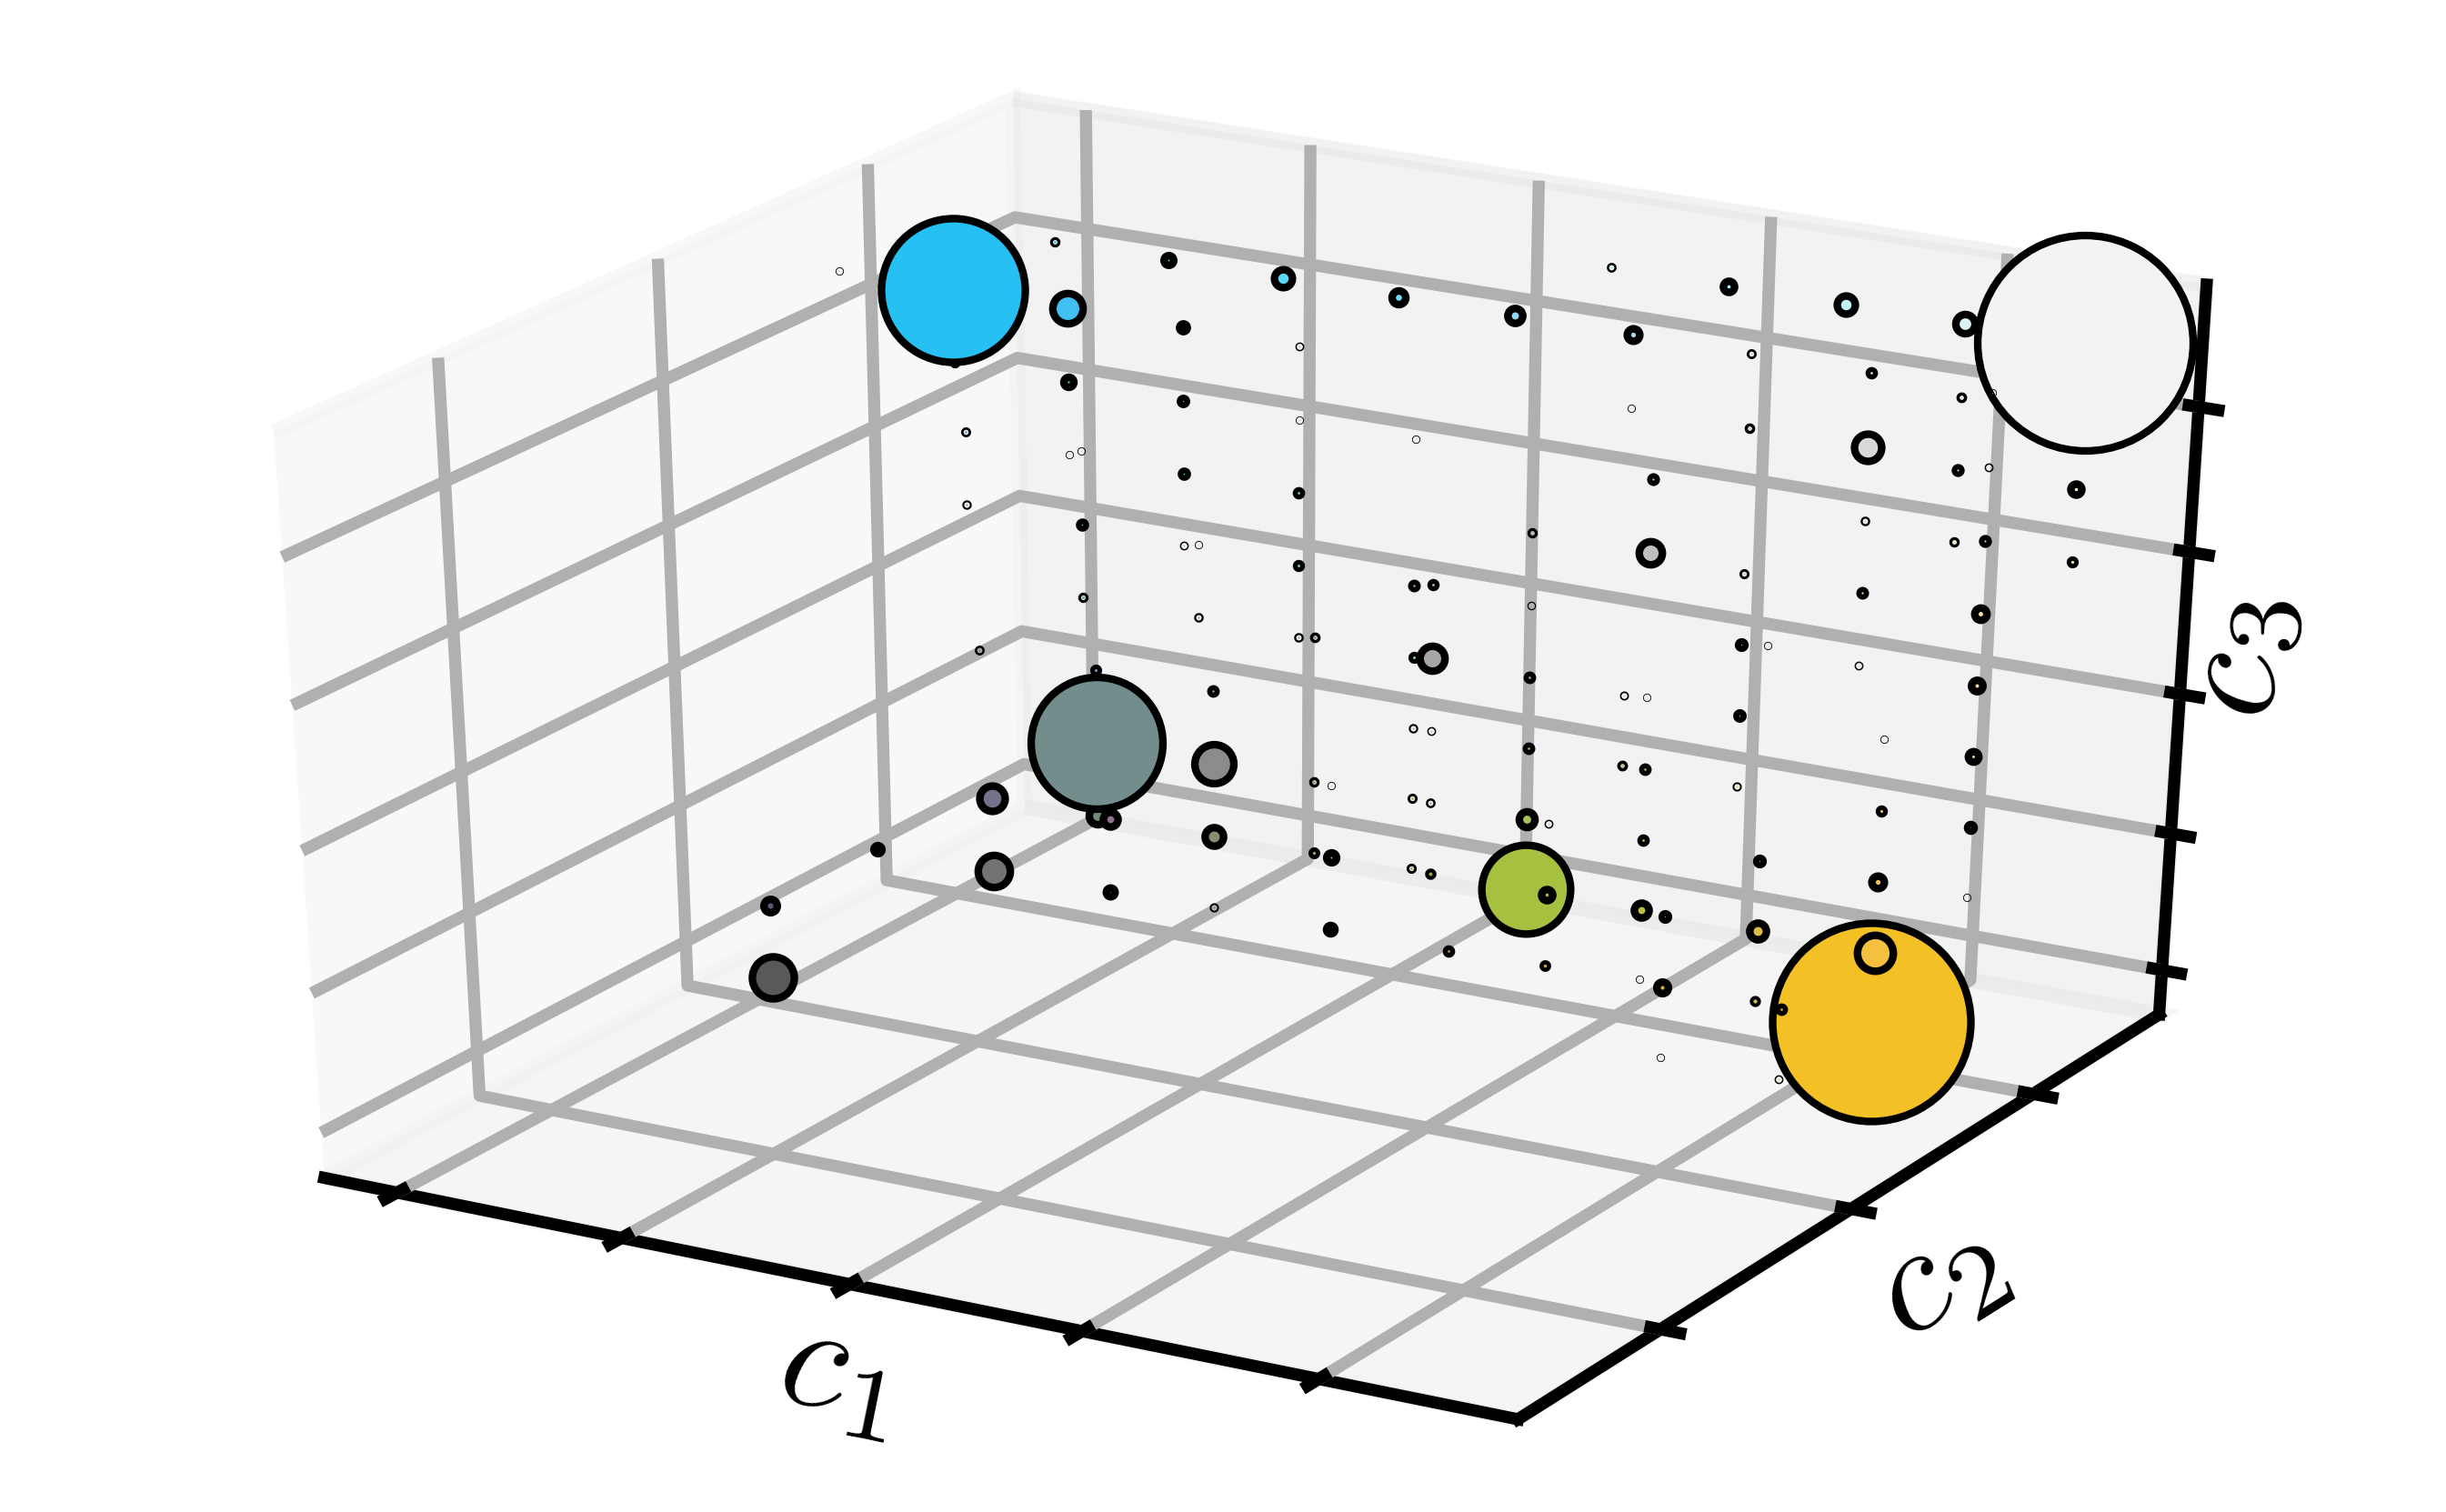
\includegraphics[width=\dimexpr\linewidth-20pt\relax]{tempo_3d_histogram}
    \end{subfigure}~ 
%    \begin{subfigure}[b]{0.32\textwidth}
%        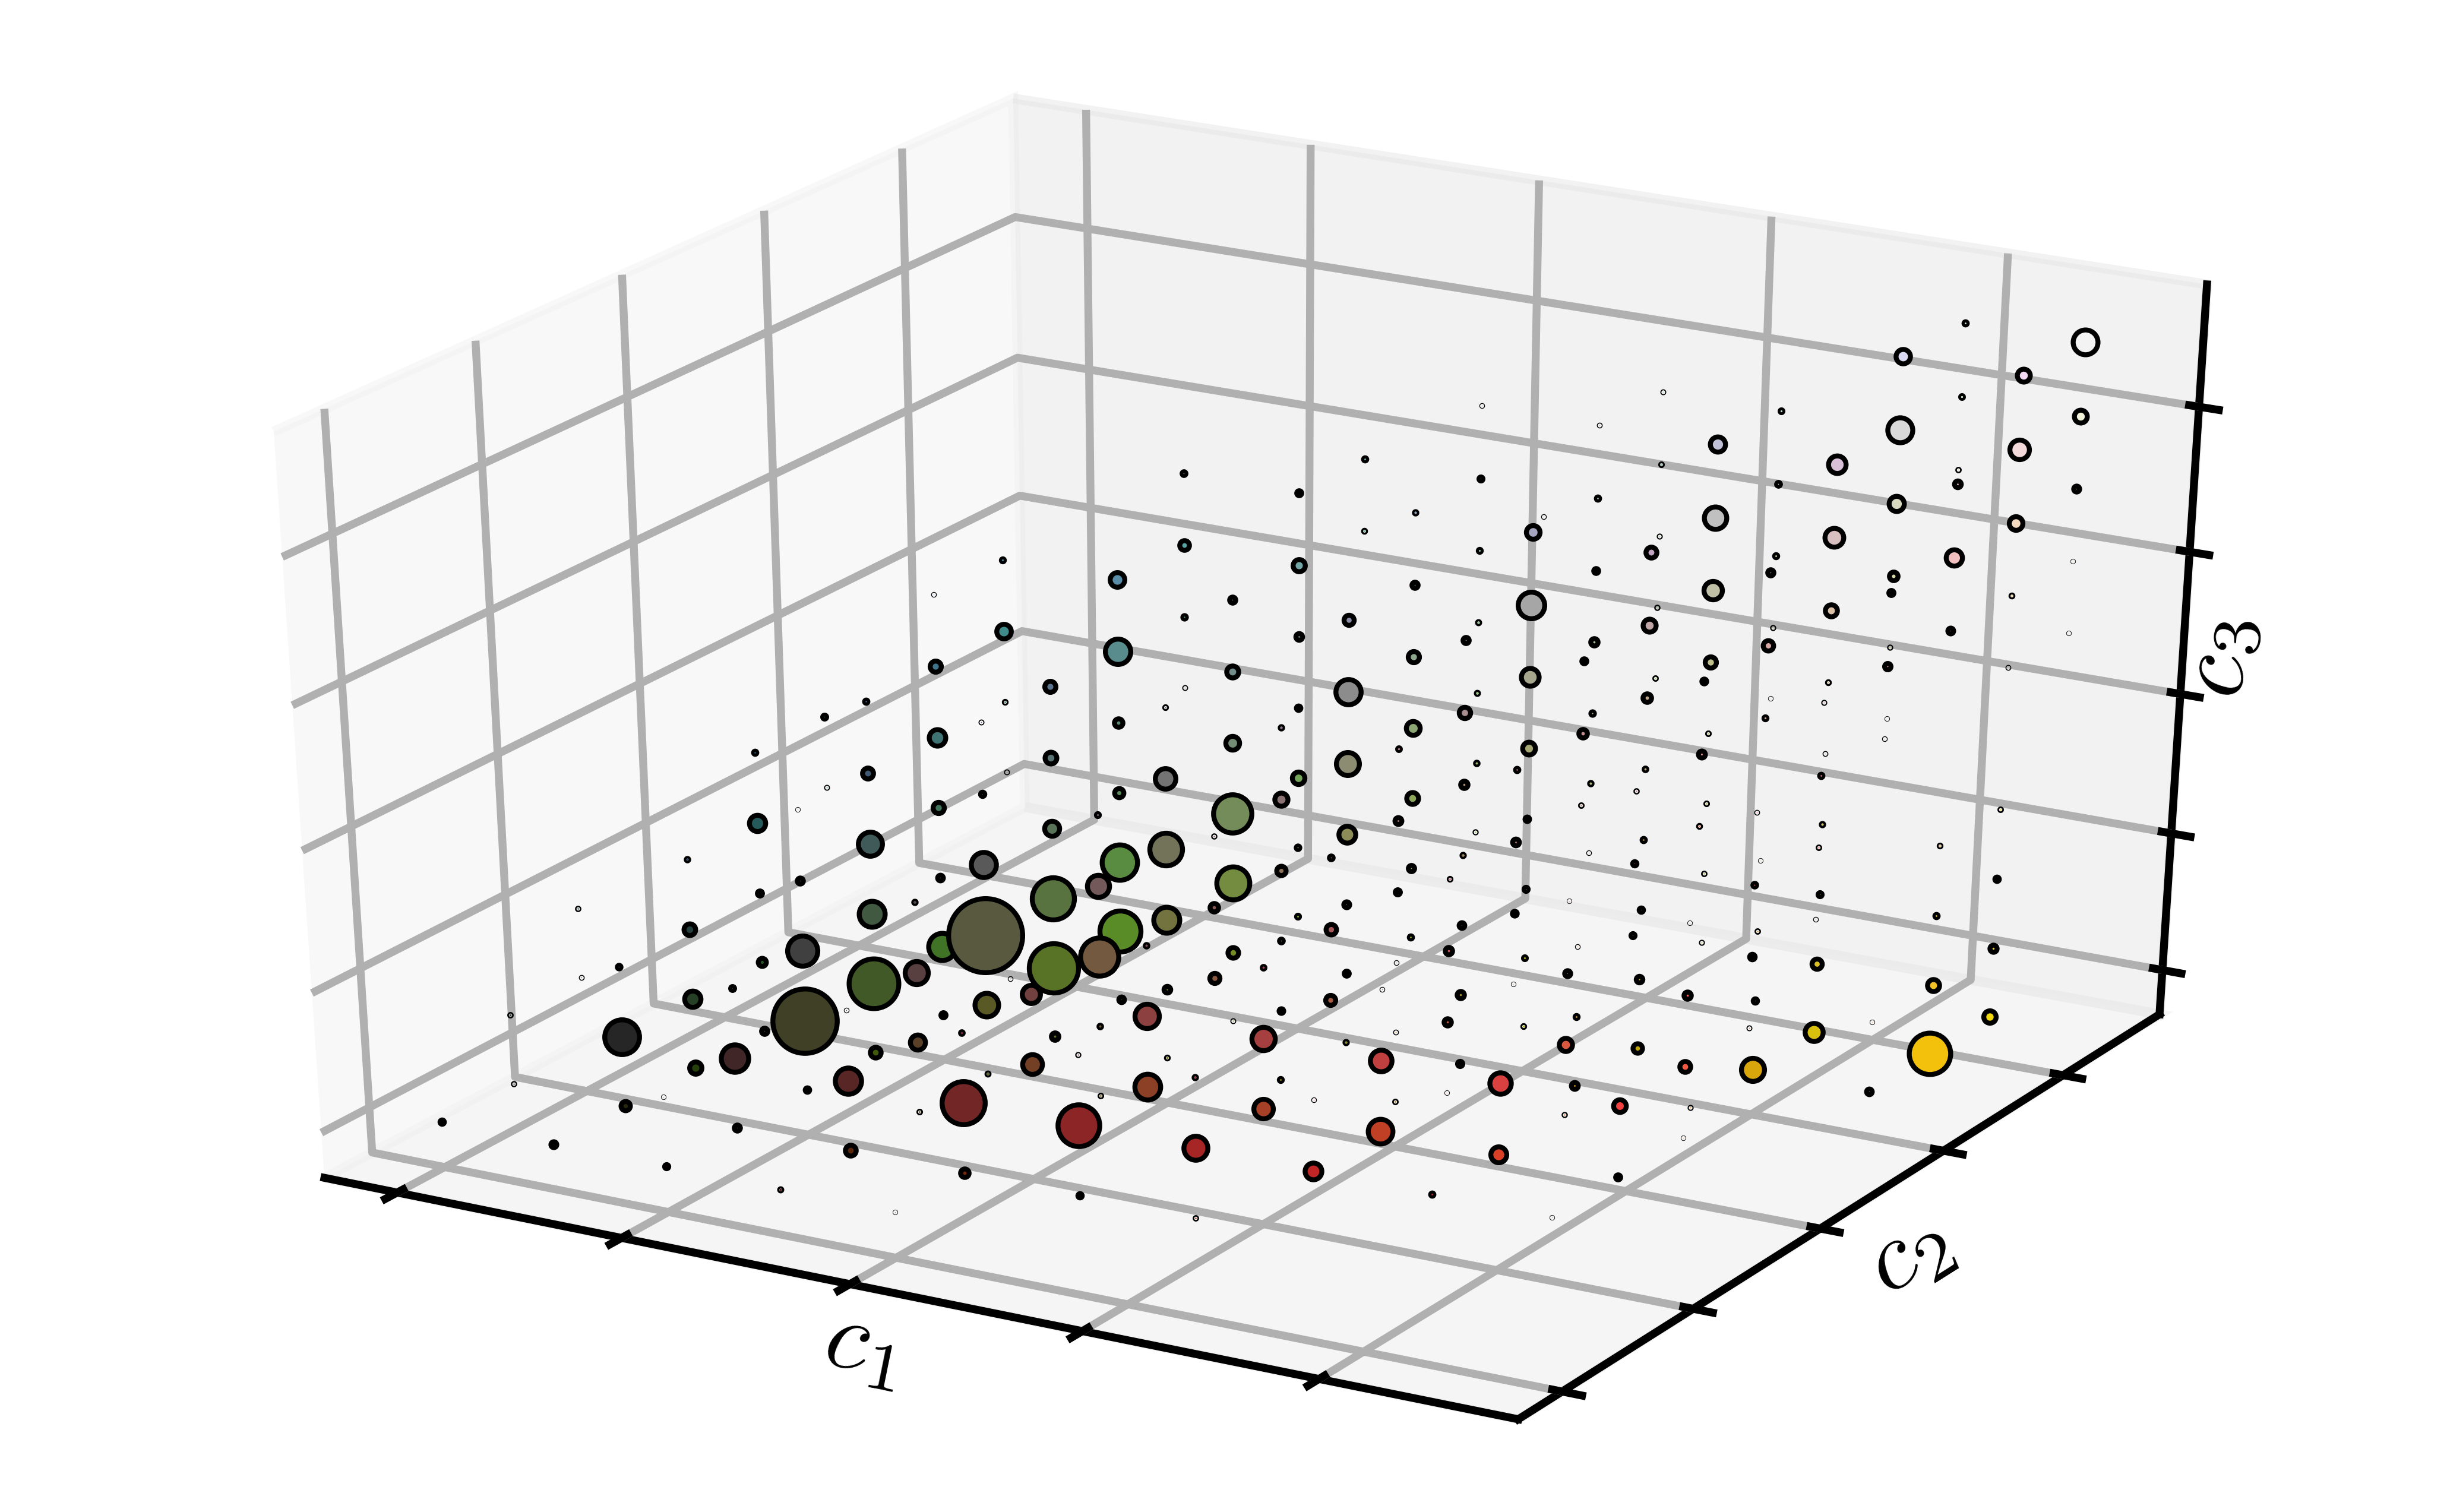
\includegraphics[width=\textwidth]{araras_3d_histogram}
%    \end{subfigure}~
    \begin{subfigure}[b]{0.32\textwidth}
        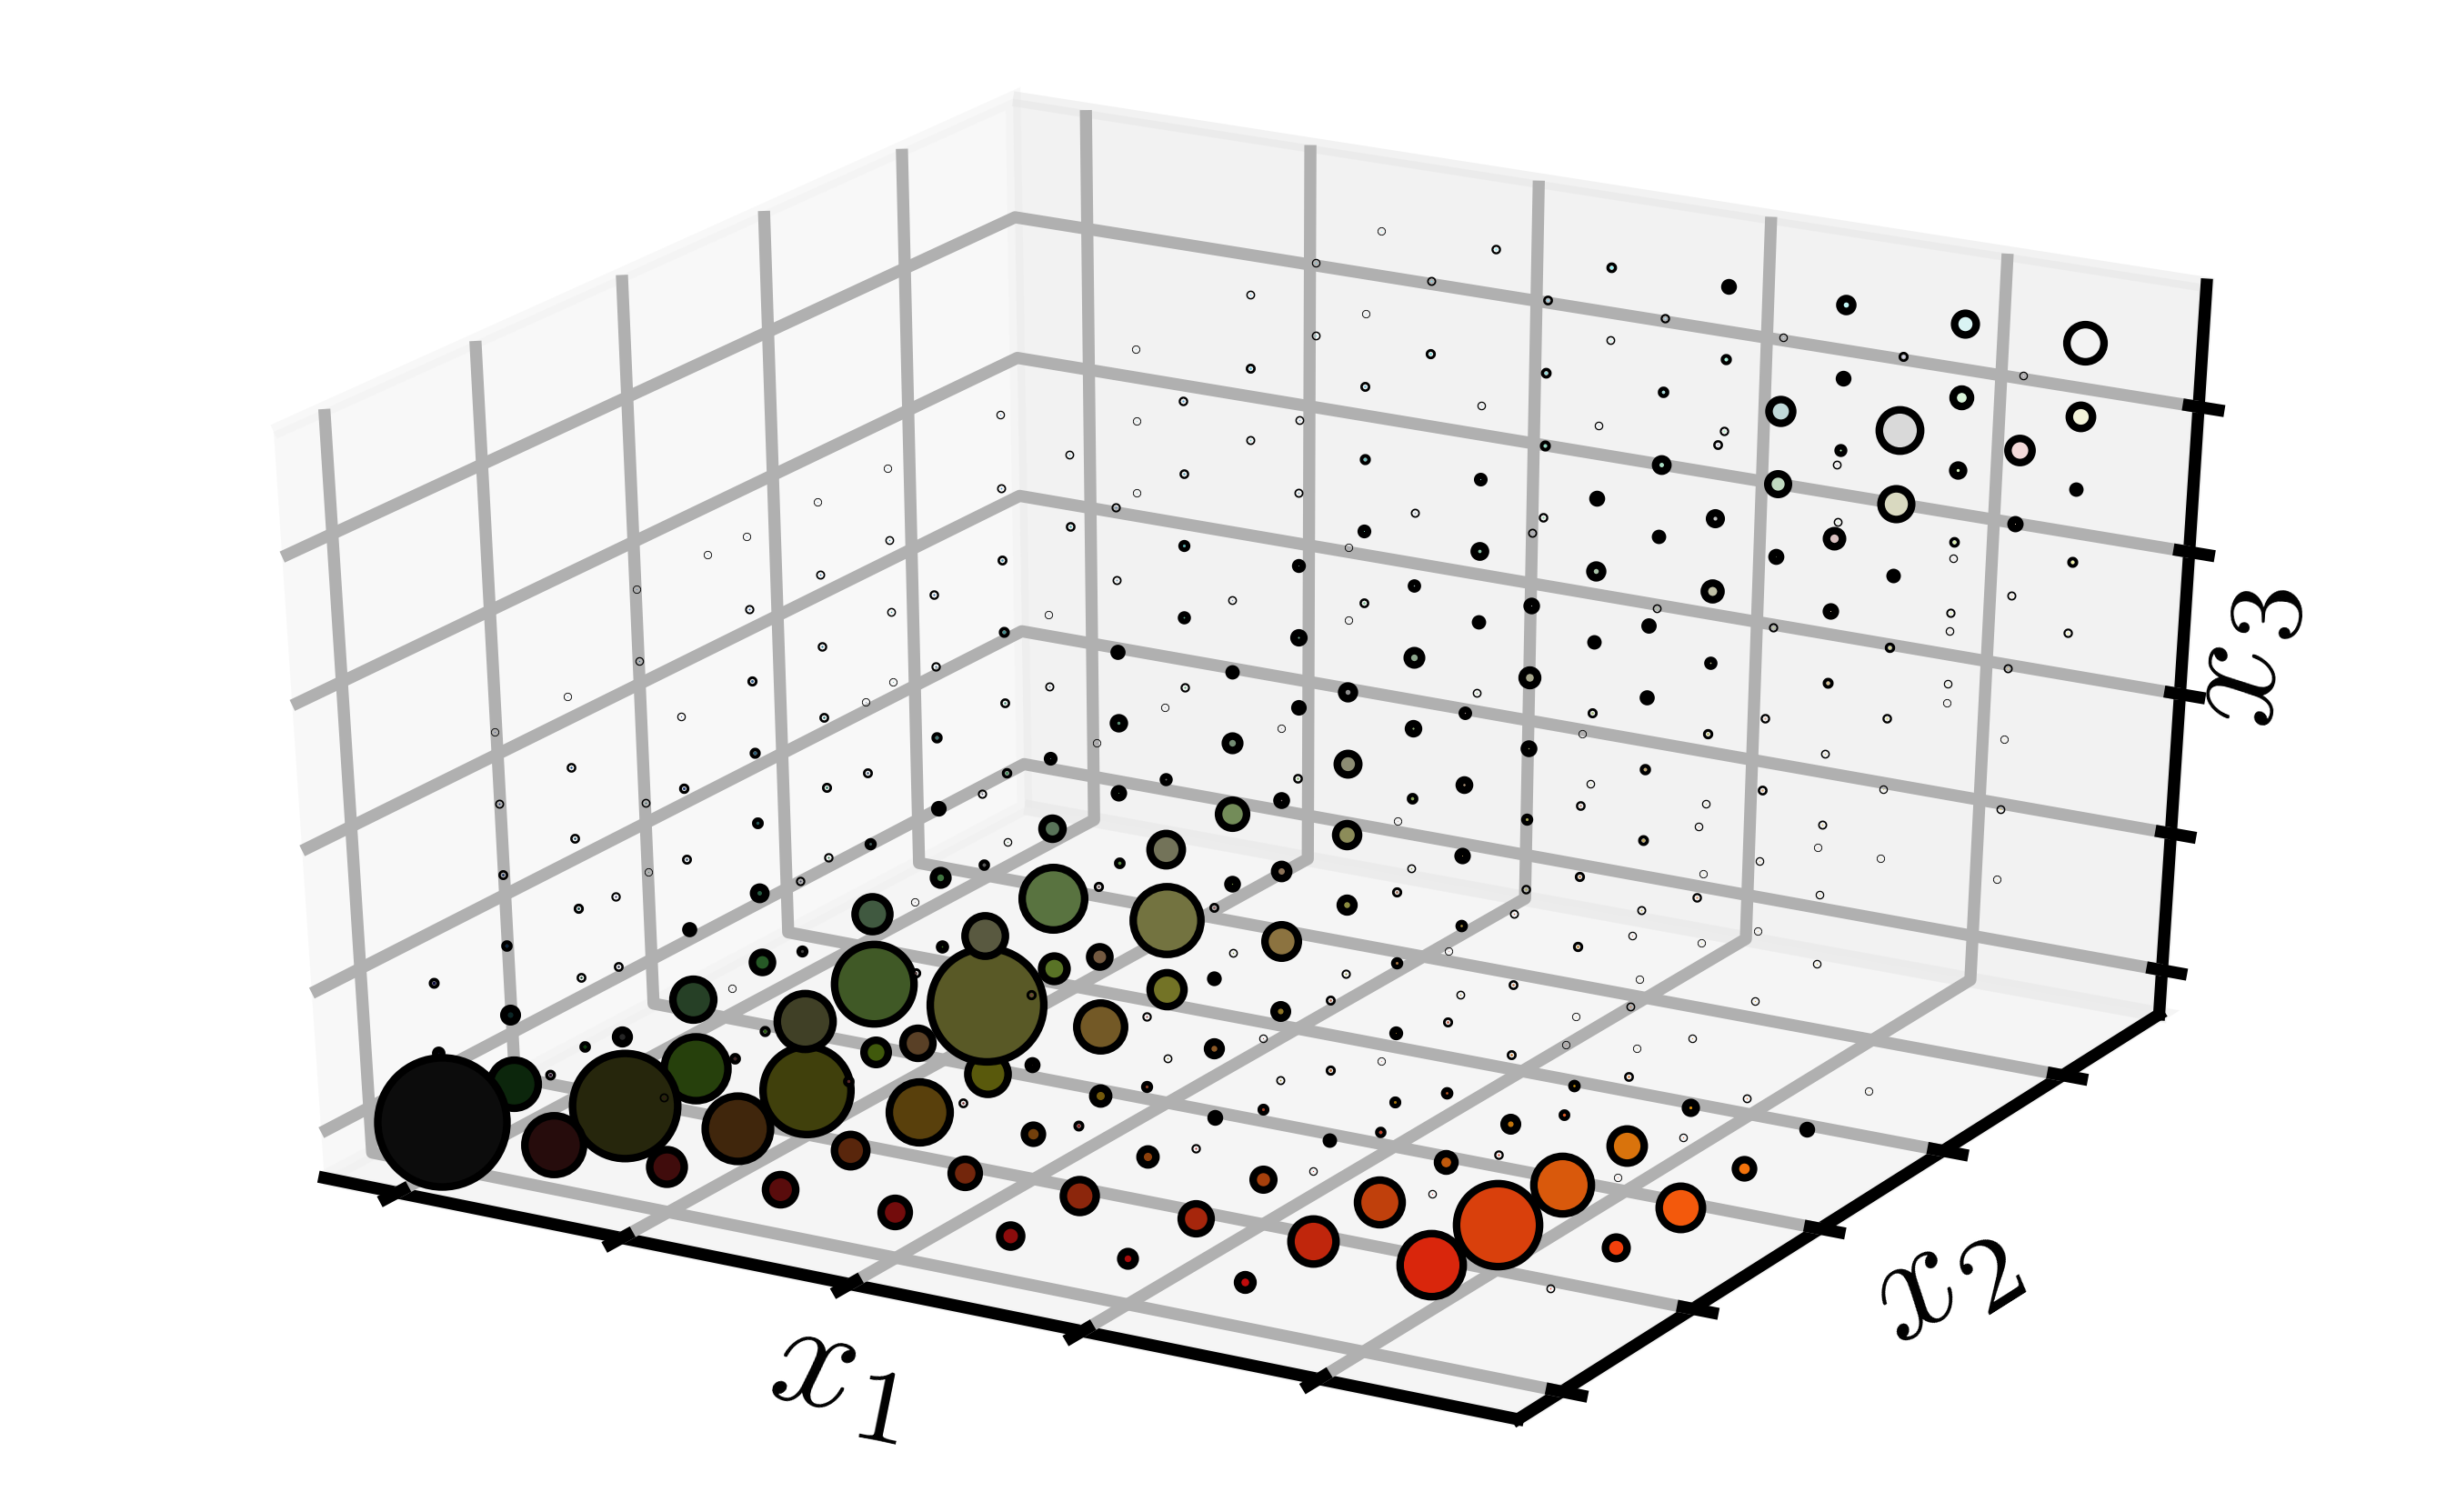
\includegraphics[width=\textwidth]{clownfish_3d_histogram}
    \end{subfigure}~
    \begin{subfigure}[b]{0.32\textwidth}
        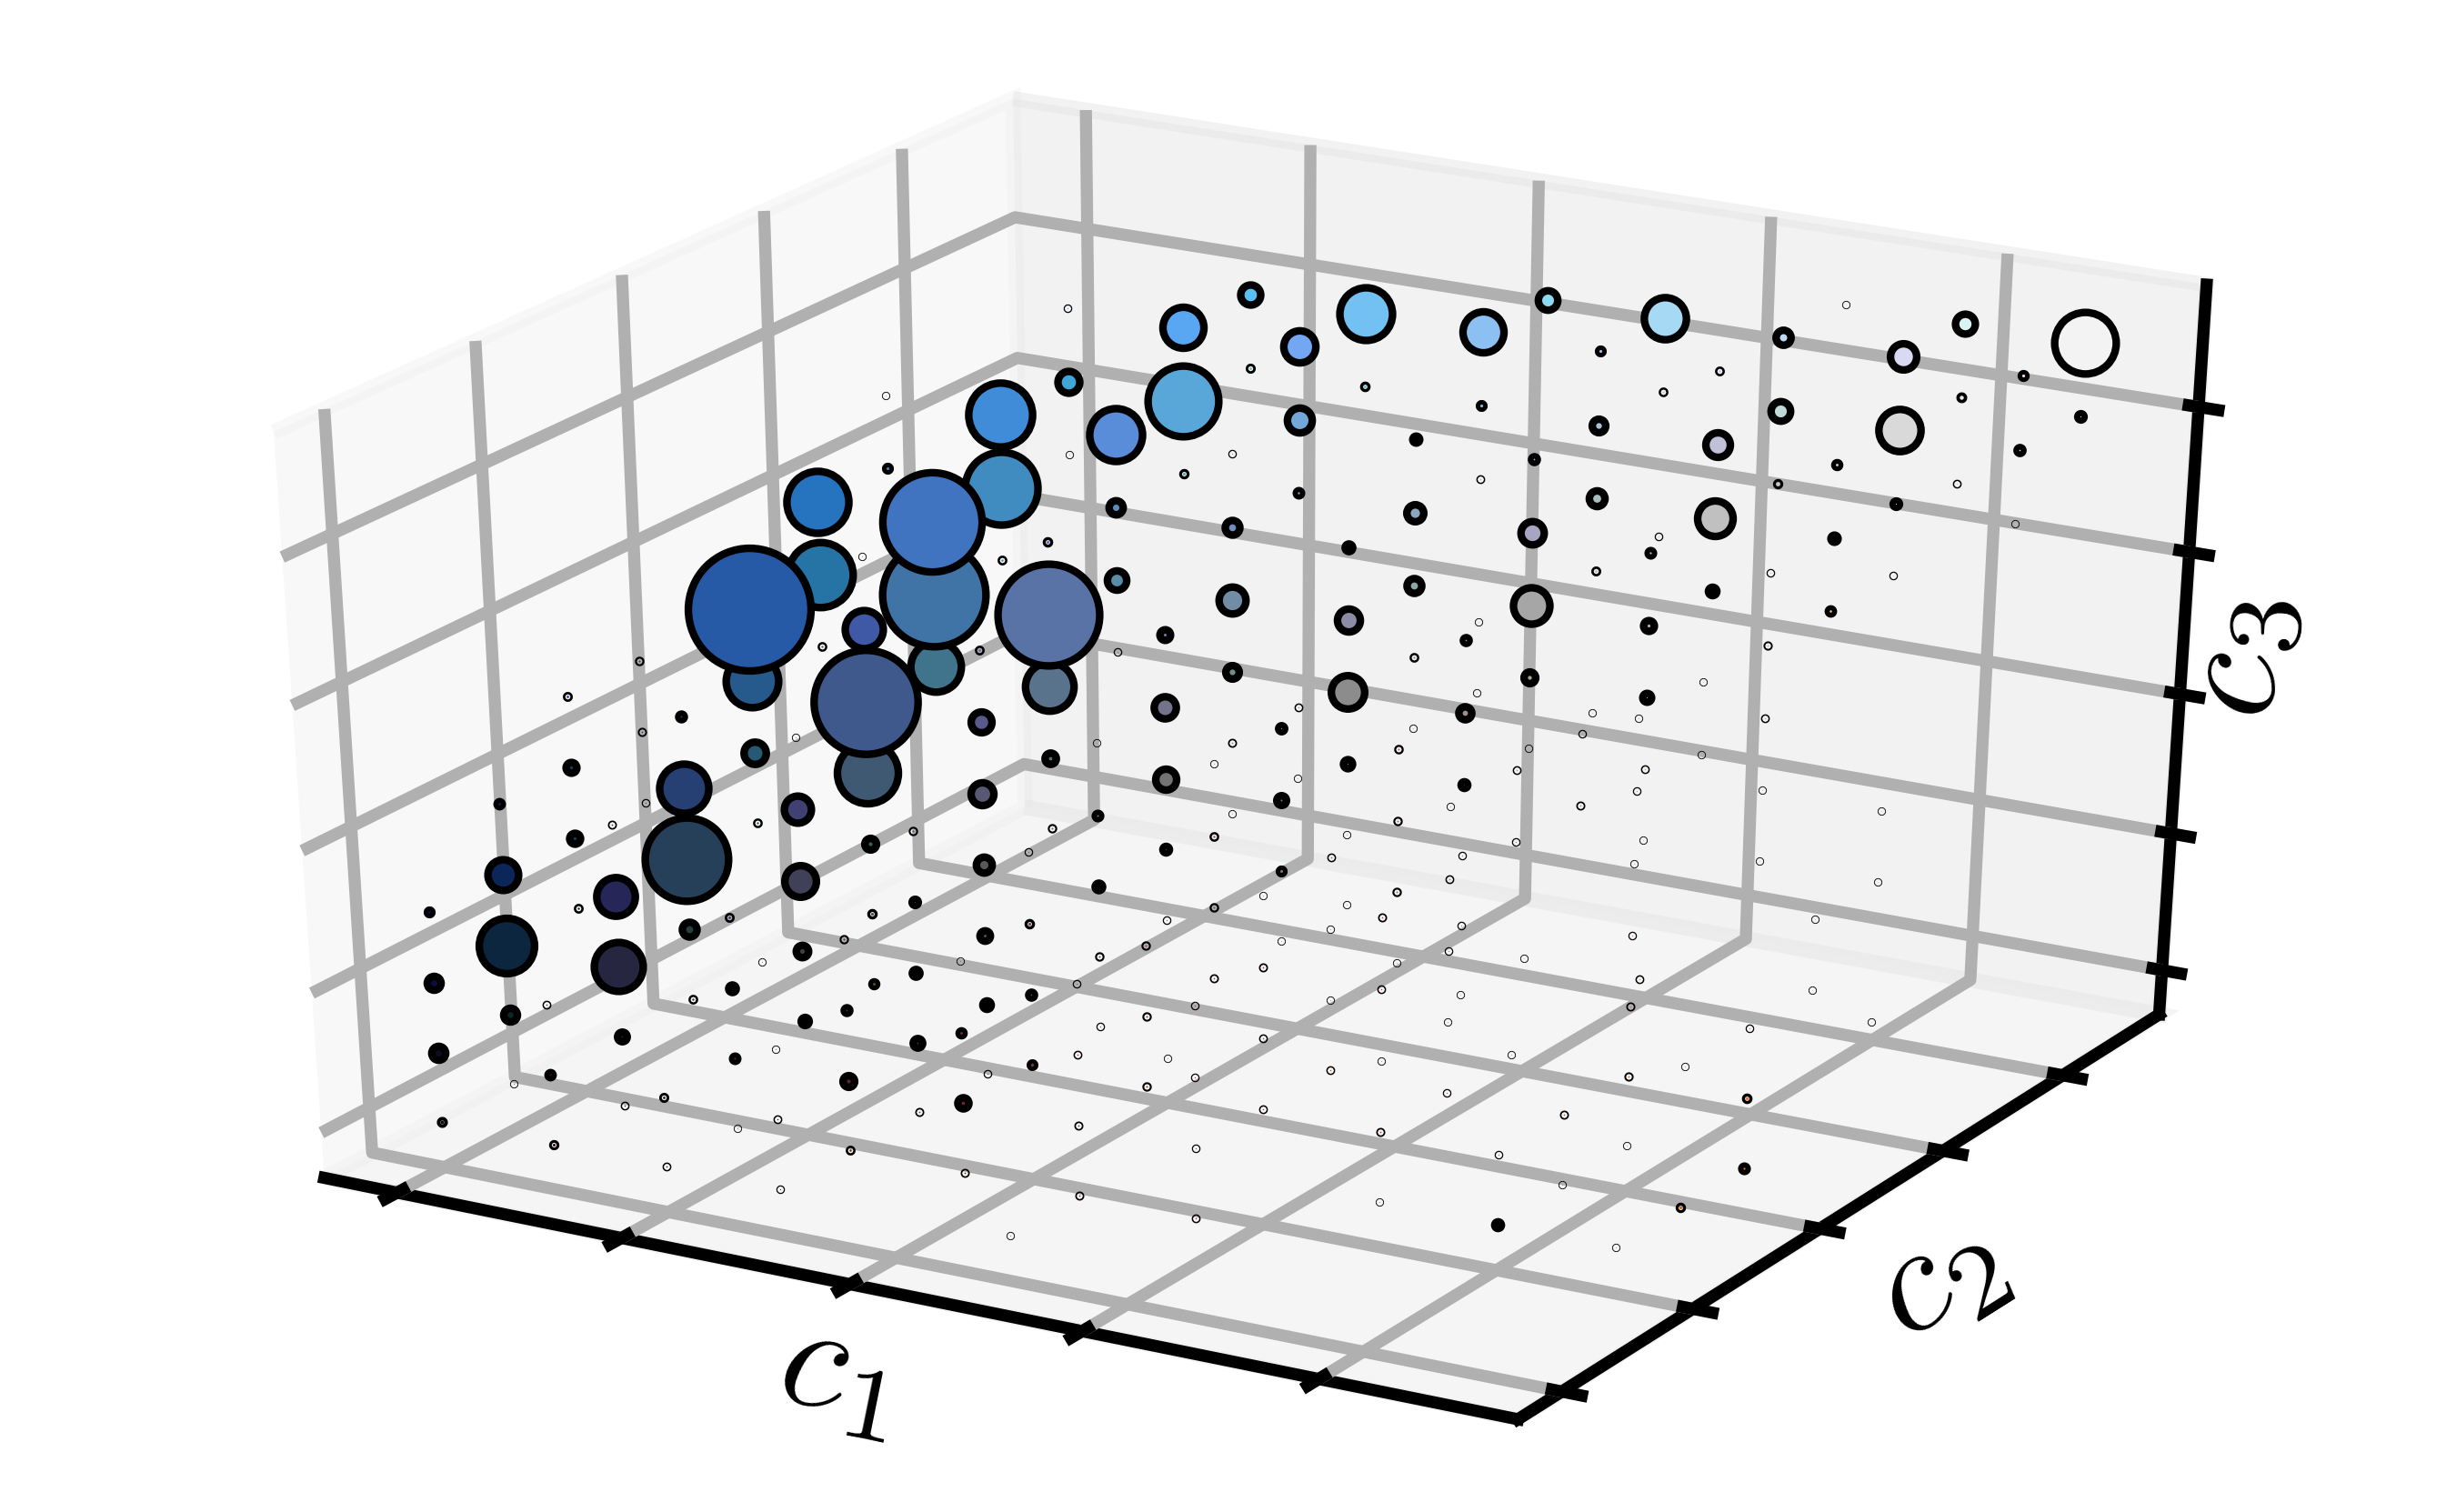
\includegraphics[width=\textwidth]{mountain_3d_histogram}
    \end{subfigure}\vspace{10pt}
    
    \begin{subfigure}[t]{\dimexpr0.32\textwidth+20pt\relax}
    	\makebox[20pt]{\raisebox{40pt}{ \small\textbf{\textsf{(e)}} }}%
    	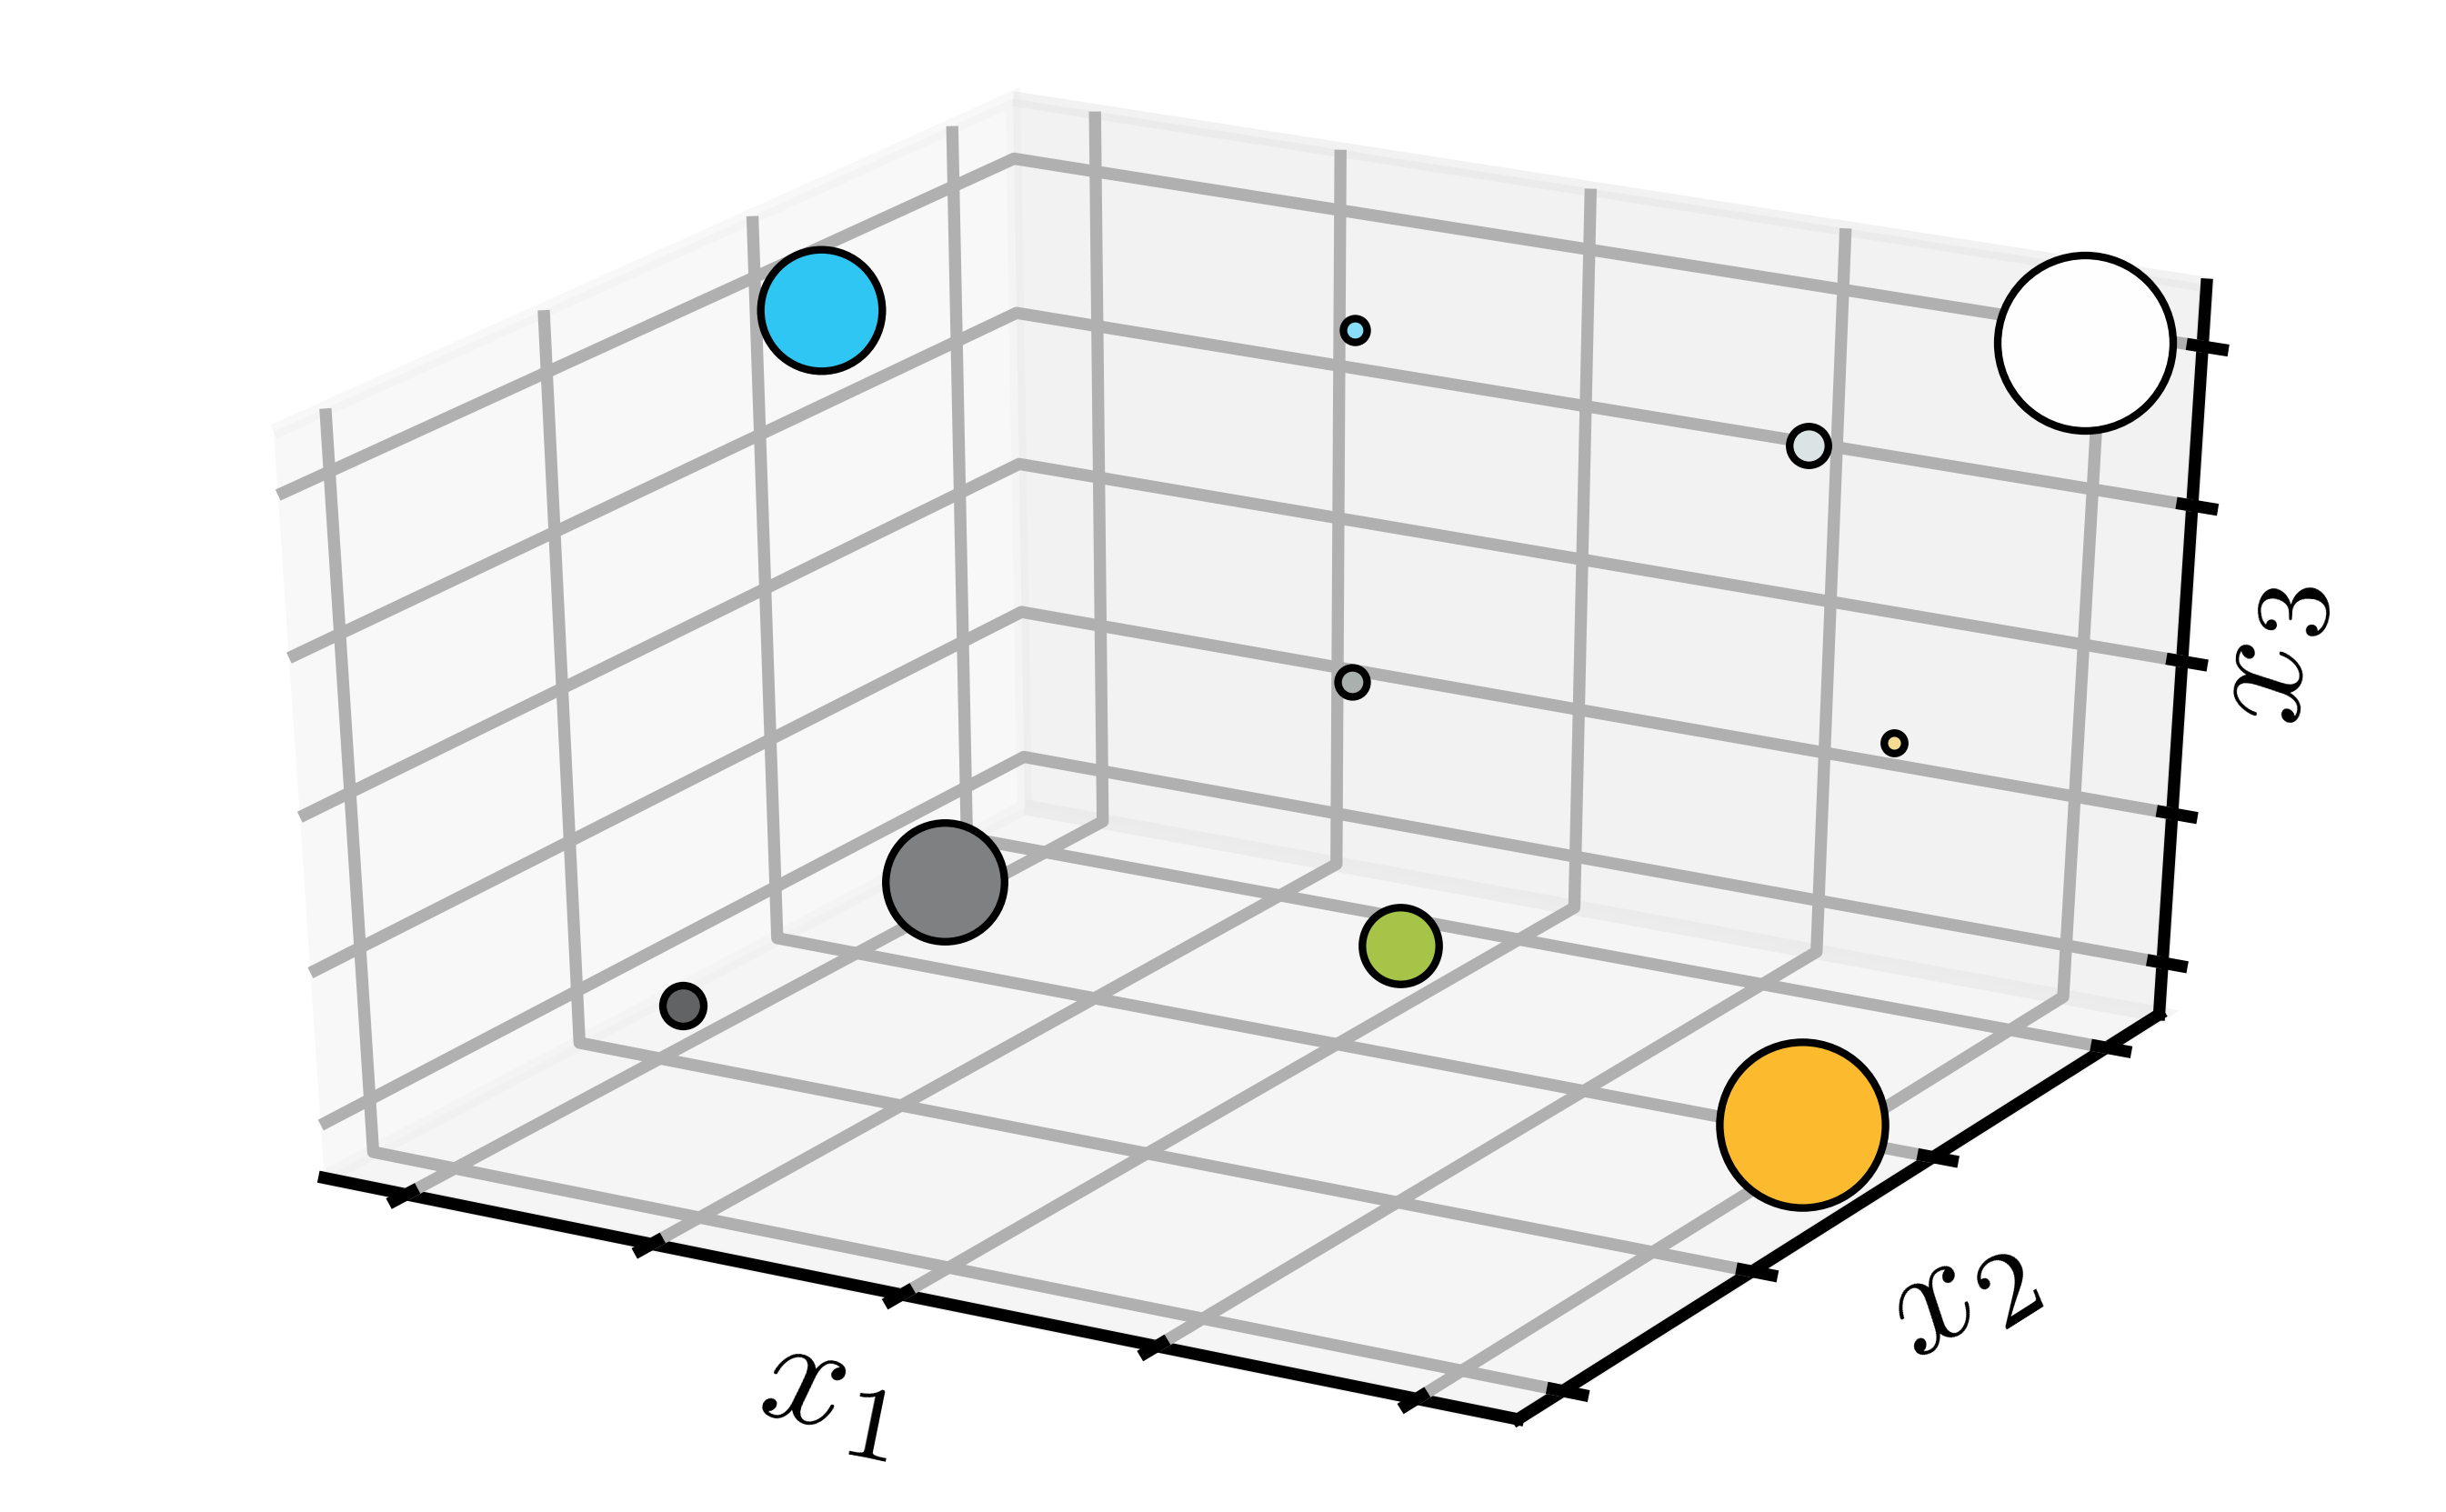
\includegraphics[width=\dimexpr\linewidth-20pt\relax]{tempo_3d_signature}
    \end{subfigure}~ 
%    \begin{subfigure}[b]{0.32\textwidth}
%        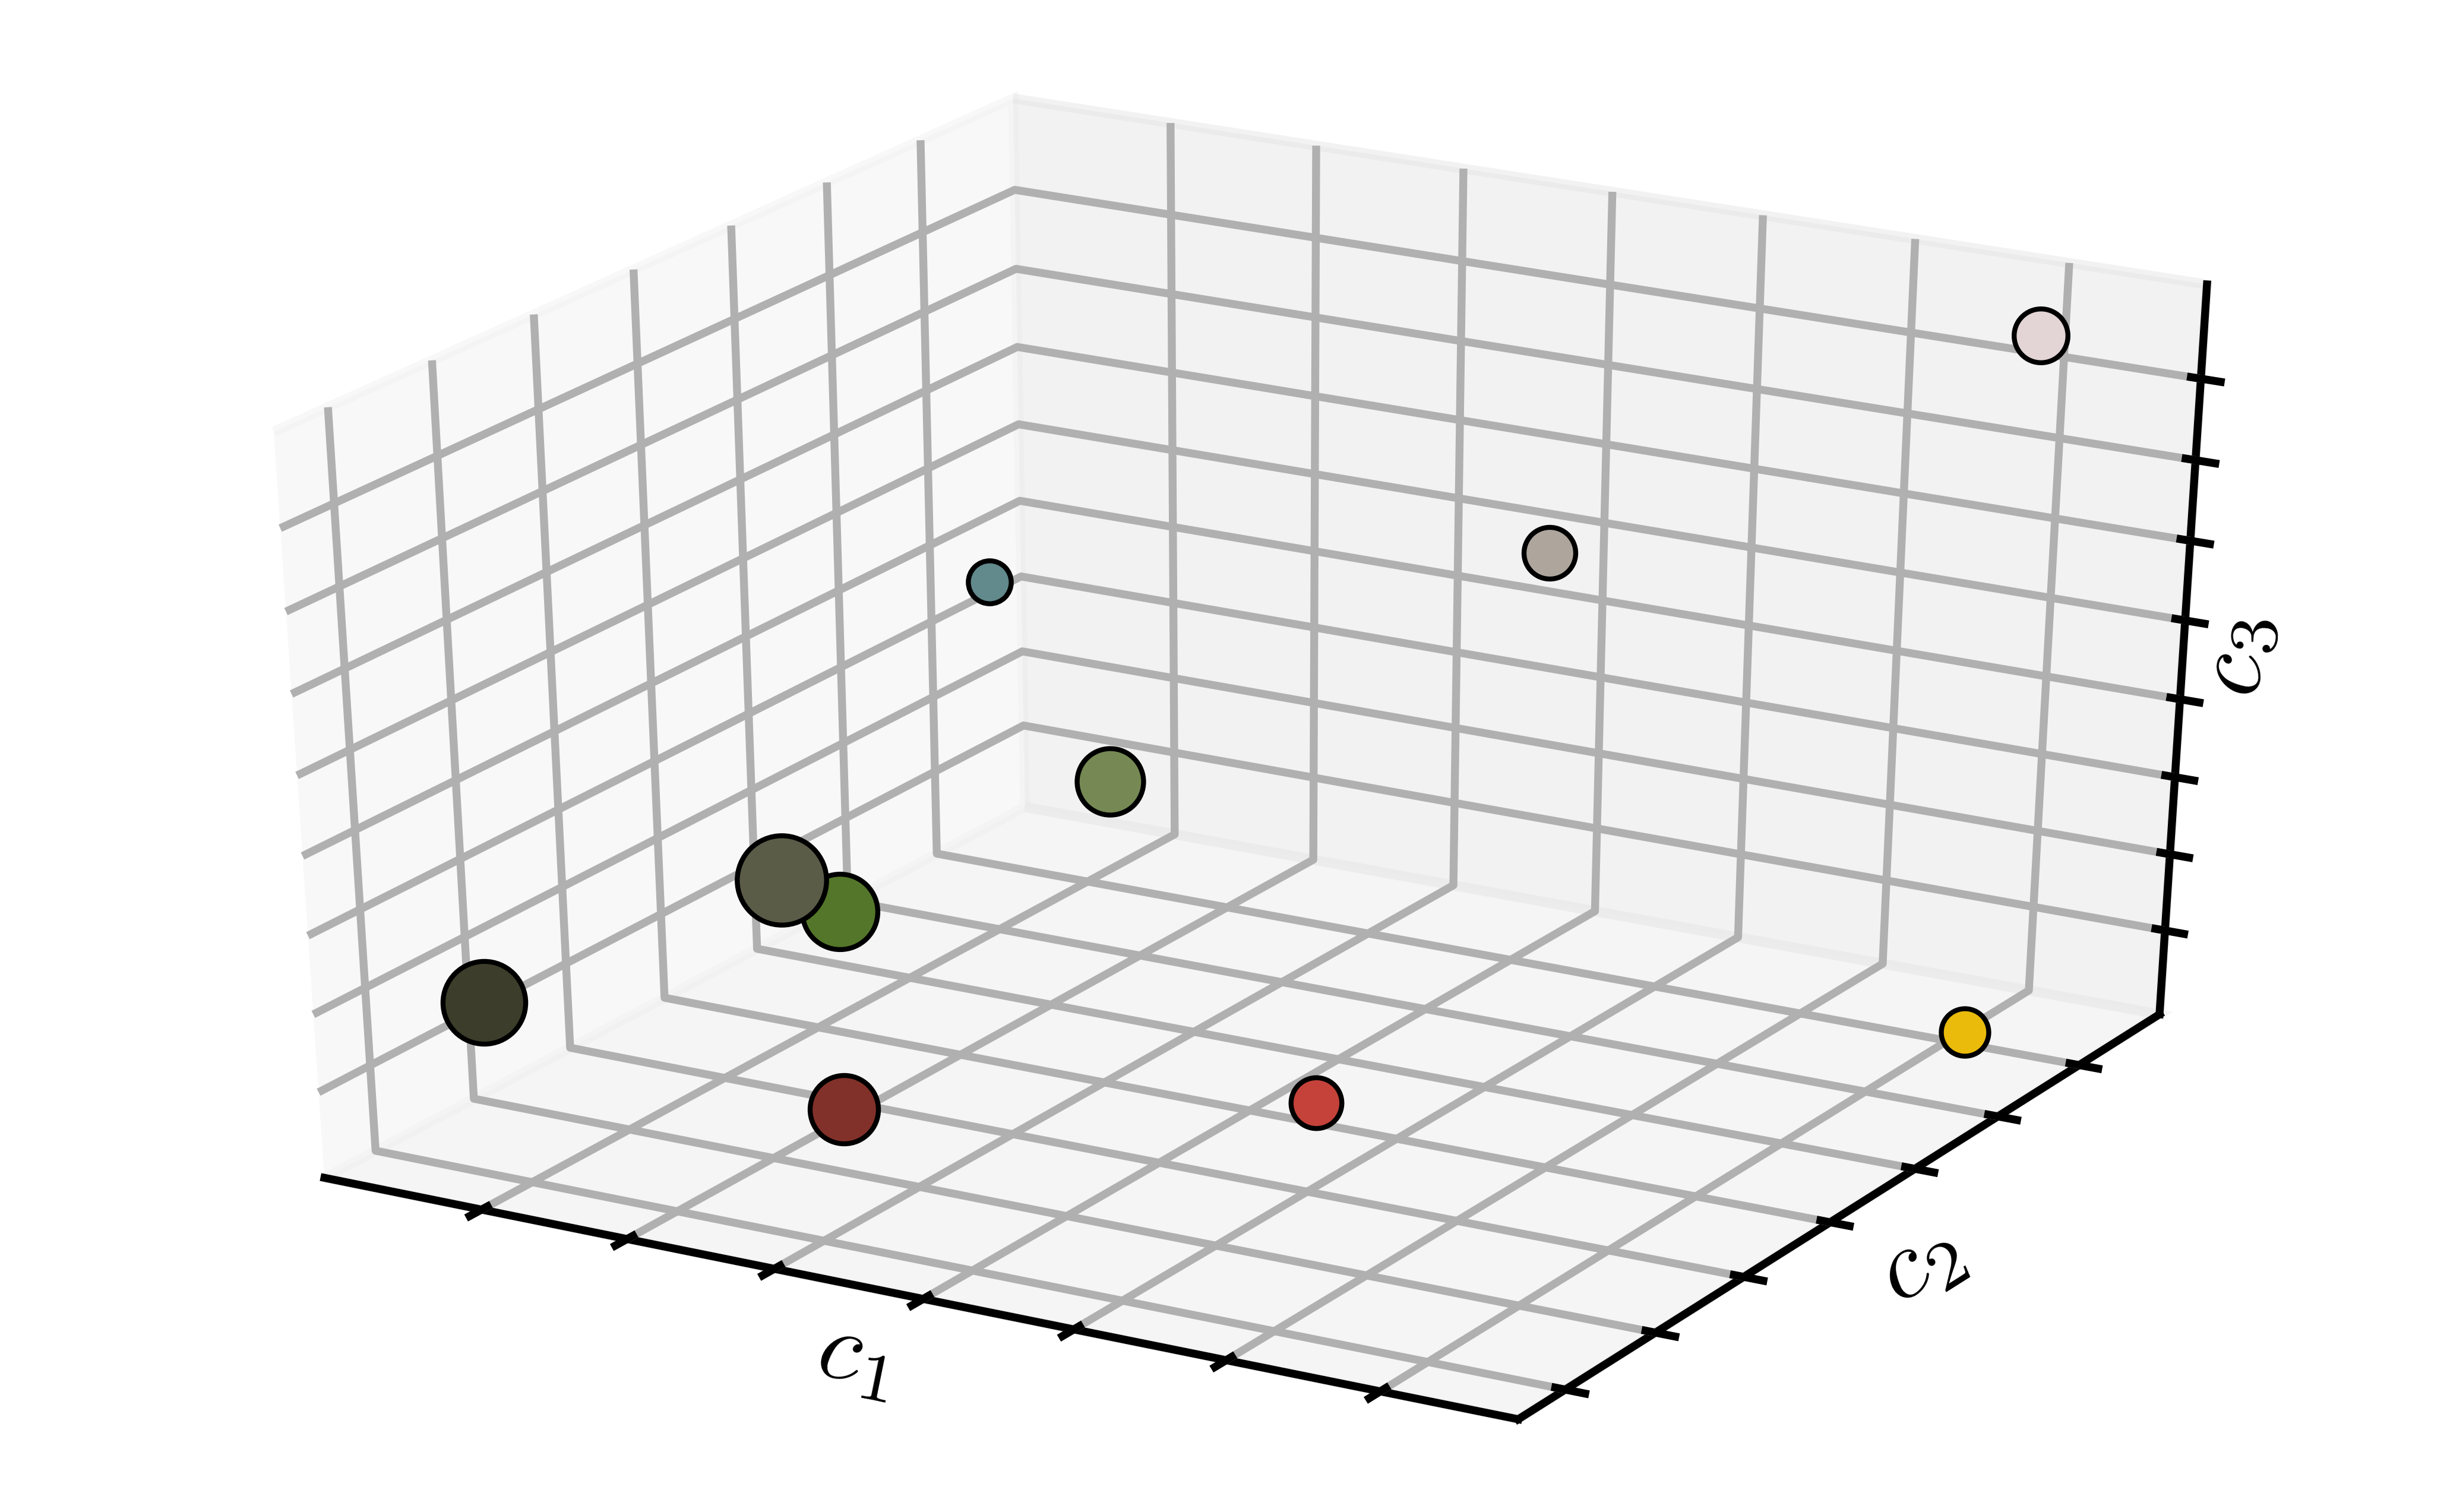
\includegraphics[width=\textwidth]{araras_3d_signature}
%    \end{subfigure}~
    \begin{subfigure}[b]{0.32\textwidth}
        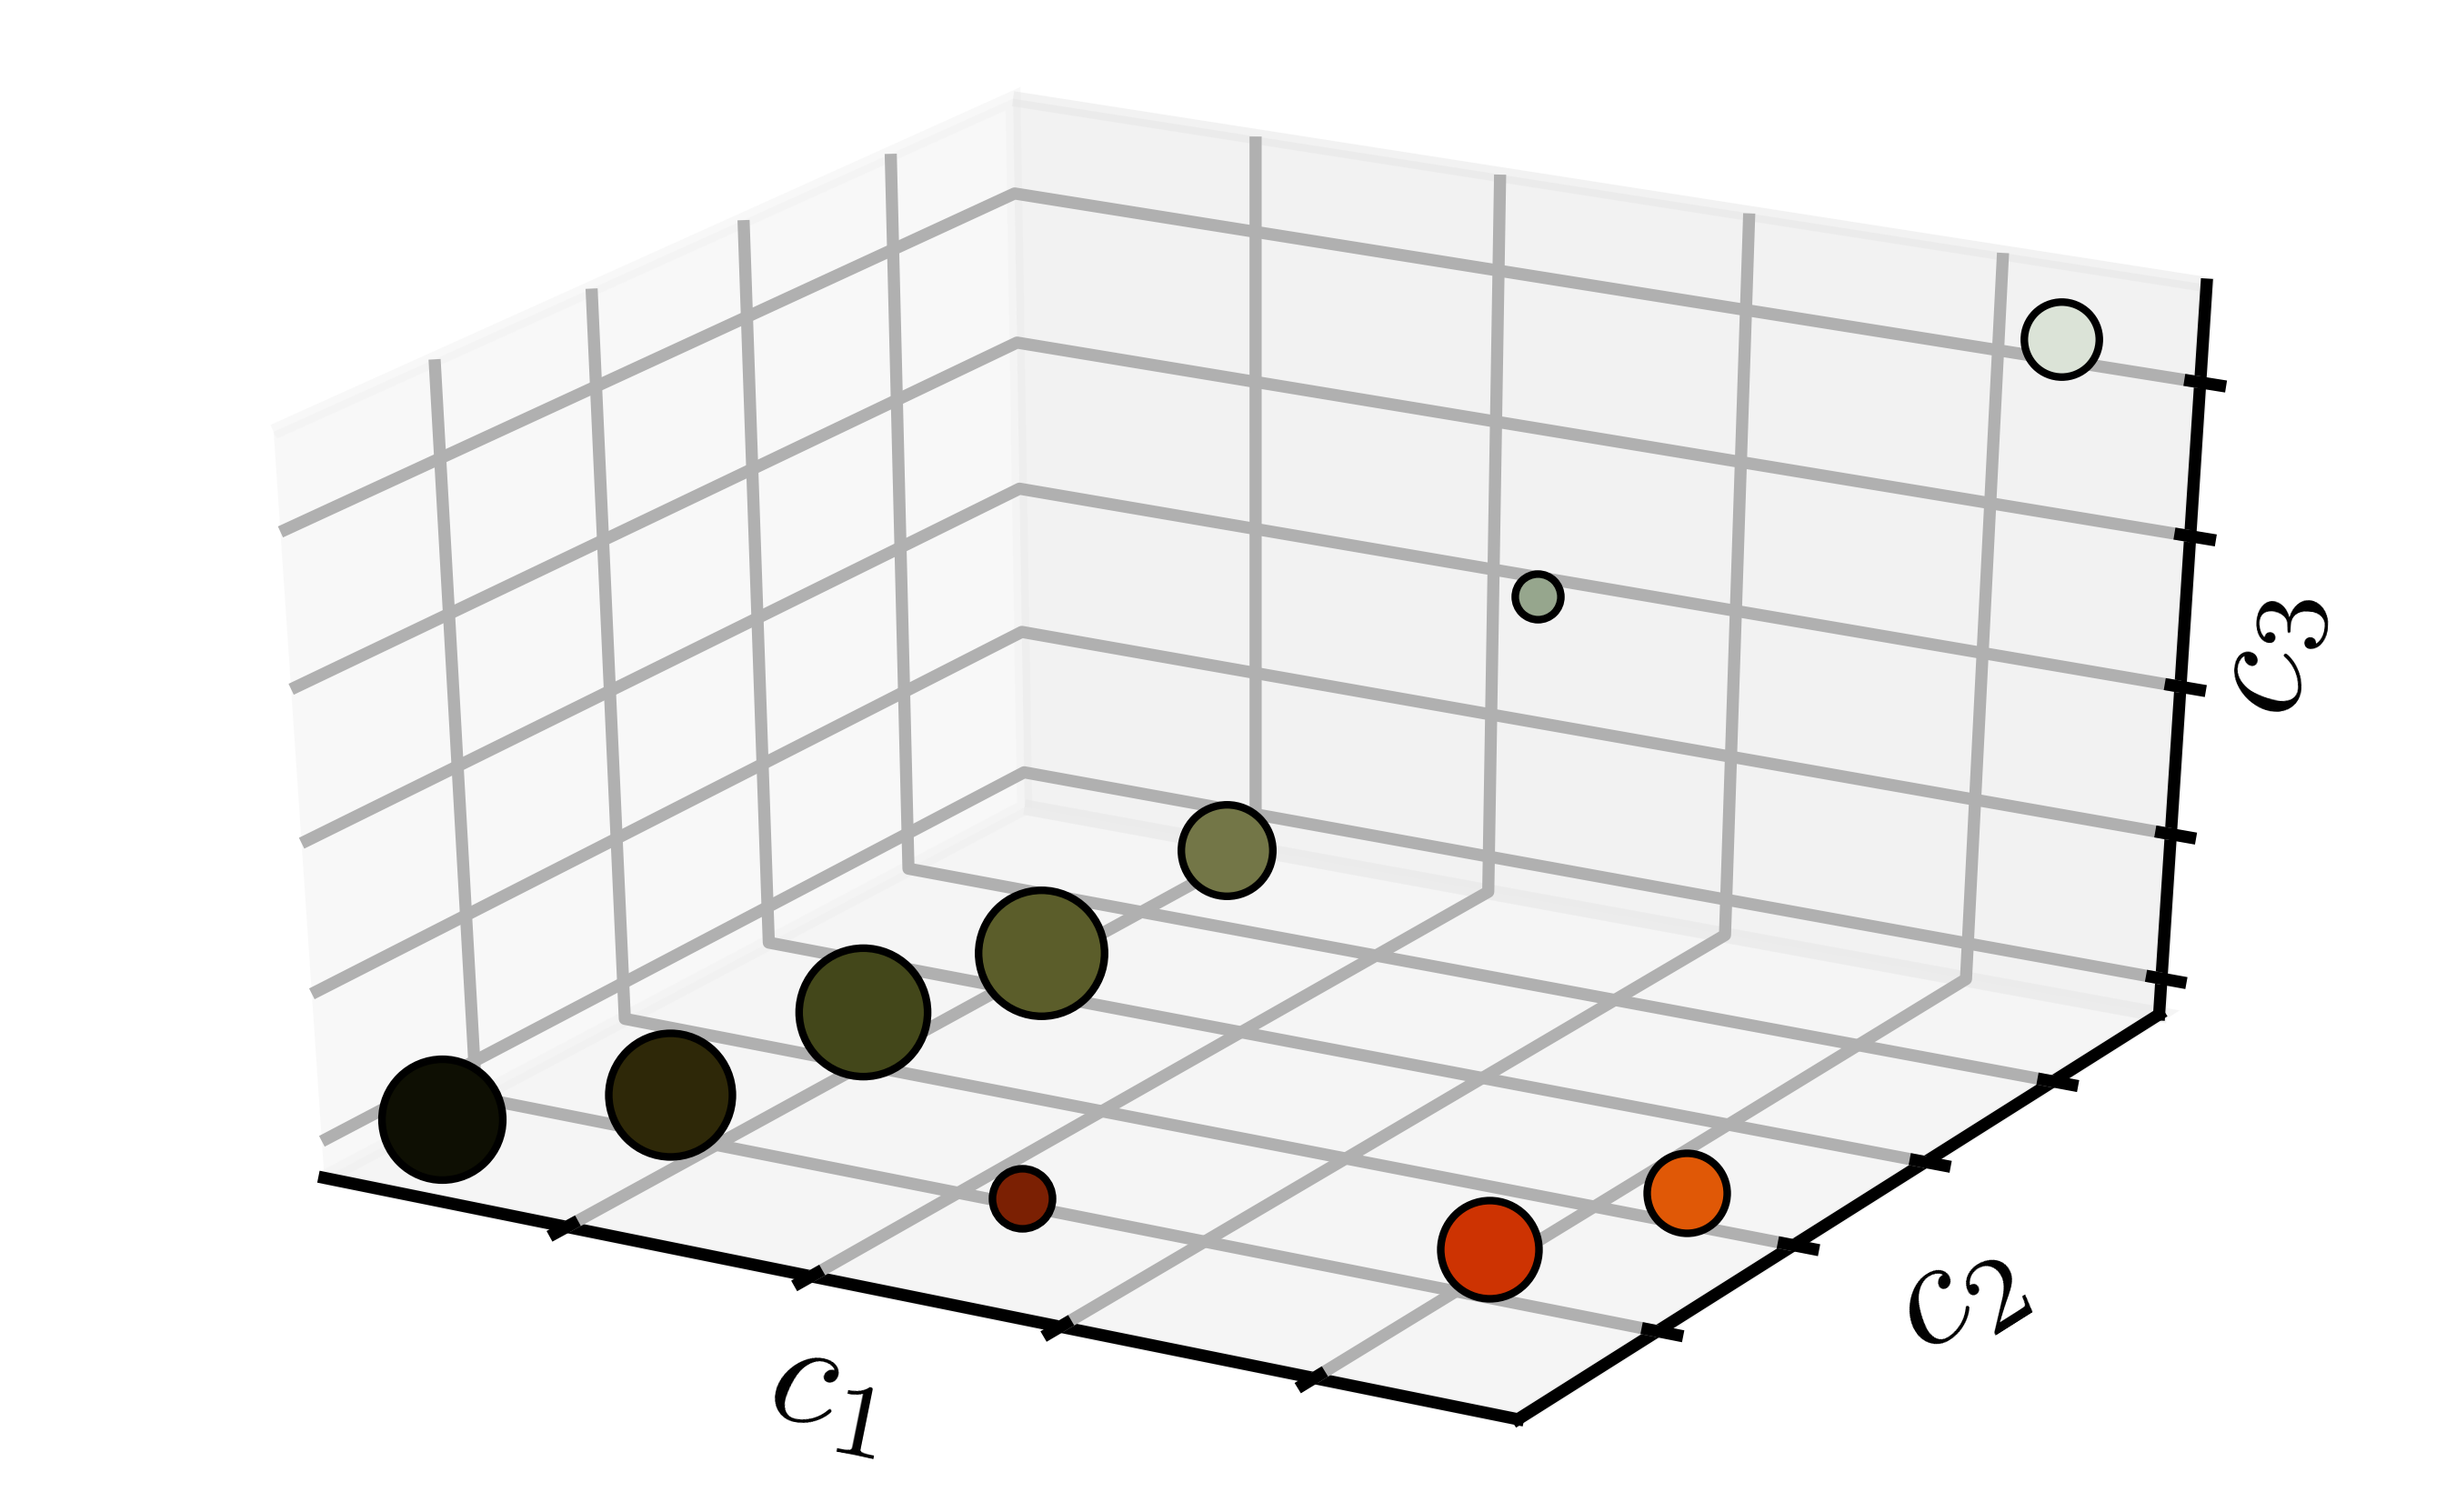
\includegraphics[width=\textwidth]{clownfish_3d_signature}
    \end{subfigure}~
    \begin{subfigure}[b]{0.32\textwidth}
        \includegraphics[width=\textwidth]{mountain_3d_signature}
    \end{subfigure}\vspace{10pt}
    
    \begin{subfigure}[t]{\dimexpr0.32\textwidth+20pt\relax}
    	\makebox[20pt]{\raisebox{40pt}{ \small\textbf{\textsf{(f)}} }}%
    	\includegraphics[width=\dimexpr\linewidth-20pt\relax]{tempo_color_clusters}
    \end{subfigure}~ 
%    \begin{subfigure}[b]{0.32\textwidth}
%        \includegraphics[width=\textwidth]{araras_color_clusters}
%    \end{subfigure}~
    \begin{subfigure}[b]{0.32\textwidth}
        \includegraphics[width=\textwidth]{clownfish_color_clusters}
    \end{subfigure}~
    \begin{subfigure}[b]{0.32\textwidth}
        \includegraphics[width=\textwidth]{mountain_color_clusters}
    \end{subfigure}\vspace{-5pt}
    
    \begin{subfigure}[t]{\dimexpr0.32\textwidth+20pt\relax}
    	\makebox[20pt]{\raisebox{25pt}{}}%
    	\includegraphics[width=\dimexpr\linewidth-20pt\relax]{tempo_bar_signature}
    \end{subfigure}~ 
%    \begin{subfigure}[b]{0.32\textwidth}
%        \includegraphics[width=\textwidth]{araras_bar_signature}
%    \end{subfigure}~
    \begin{subfigure}[b]{0.32\textwidth}
        \includegraphics[width=\textwidth]{clownfish_bar_signature}
    \end{subfigure}~
    \begin{subfigure}[b]{0.32\textwidth}
        \includegraphics[width=\textwidth]{mountain_bar_signature}
    \end{subfigure}
                    
	\caption{Different representations of color information. {\small \textsf{\textbf{(a)}}} input color image , {\small \textsf{\textbf{(b)}}} single-channel color histogram , {\small \textsf{\textbf{(c)}}} 3-d color distribution , {\small \textsf{\textbf{(d)}}} 3-d color histogram , {\small \textsf{\textbf{(e)}}} 3-d color signature , {\small \textsf{\textbf{(f)}}} color signature clusters .}\label{fig:color_image_representations}    
\end{figure}


\section{Texture}

\section{Texture characterization}

\begin{figure}[!ht]
    \centering
    \begin{subfigure}[b]{0.19\textwidth}
        \includegraphics[width=\textwidth]{brodatz_skin}
        \caption{}
    \end{subfigure}
    %~ %add desired spacing between images, e. g. ~, \quad, \qquad, \hfill etc. 
      %(or a blank line to force the subfigure onto a new line)
    \begin{subfigure}[b]{0.19\textwidth}
        \includegraphics[width=\textwidth]{brodatz_three}
        \caption{}
    \end{subfigure} 
    %~ %add desired spacing between images, e. g. ~, \quad, \qquad, \hfill etc. 
      %(or a blank line to force the subfigure onto a new line)    
    \begin{subfigure}[b]{0.19\textwidth}
        \includegraphics[width=\textwidth]{brodatz_wall}
        \caption{}
    \end{subfigure}
    %~ %add desired spacing between images, e. g. ~, \quad, \qquad, \hfill etc. 
      %(or a blank line to force the subfigure onto a new line)
    \begin{subfigure}[b]{0.19\textwidth}
        \includegraphics[width=\textwidth]{brodatz_vlines}
        \caption{}
    \end{subfigure}
    %~ %add desired spacing between images, e. g. ~, \quad, \qquad, \hfill etc. 
      %(or a blank line to force the subfigure onto a new line)
    \begin{subfigure}[b]{0.19\textwidth}
        \includegraphics[width=\textwidth]{brodatz_sponge}
        \caption{}
    \end{subfigure}\\
    
    \begin{subfigure}[b]{0.19\textwidth}
        \includegraphics[width=\textwidth]{brodatz_tissue}
        \caption{}
    \end{subfigure}
    %~ %add desired spacing between images, e. g. ~, \quad, \qquad, \hfill etc. 
      %(or a blank line to force the subfigure onto a new line)
    \begin{subfigure}[b]{0.19\textwidth}
        \includegraphics[width=\textwidth]{brodatz_cafe}
        \caption{}
    \end{subfigure} 
    %~ %add desired spacing between images, e. g. ~, \quad, \qquad, \hfill etc. 
      %(or a blank line to force the subfigure onto a new line)    
    \begin{subfigure}[b]{0.19\textwidth}
        \includegraphics[width=\textwidth]{brodatz_crystal}
        \caption{}
    \end{subfigure}
    %~ %add desired spacing between images, e. g. ~, \quad, \qquad, \hfill etc. 
      %(or a blank line to force the subfigure onto a new line)
    \begin{subfigure}[b]{0.19\textwidth}
        \includegraphics[width=\textwidth]{brodatz_flowers}
        \caption{}
    \end{subfigure}
    %~ %add desired spacing between images, e. g. ~, \quad, \qquad, \hfill etc. 
      %(or a blank line to force the subfigure onto a new line)
    \begin{subfigure}[b]{0.19\textwidth}
        \includegraphics[width=\textwidth]{brodatz_paint}
        \caption{}
    \end{subfigure}    
                  
    \caption{ Examples of texture images and its classification. [{\small \textsf{\textbf{(a) (b) (e) (h)}}}] nautural textures, [{\small \textsf{\textbf{(c) (d) (f) (g) (i) (j)}}}] man-made textures, [{\small \textsf{\textbf{(c) (d)}}}] regular textures, [{\small \textsf{\textbf{(g) (h)}}}] stochastic textures, [{\small \textsf{\textbf{(c) (d)}}}] homogeneous, [{\small \textsf{\textbf{(a) (b) (f) (g) (h)}}}] weakly-homogeneous, [{\small \textsf{\textbf{(i) (j)}}}] inhomogeneous.}\label{fig:texture_images}    
\end{figure}


\begin{itemize}
	\item Natural and artificial 
	\item Regular, stochastic
	\item Homogeneous, non-homogeneous, in-homogeneous
\end{itemize}



There is a disagreement in the definition of texture in the field of computer vision. It is possible to give a mathematical definition based on its statistical properties, however, these properties are very imprecise and/or restrictive to adapt to the diversity of existing textures.

The definition that we support is based on an experimental finding: a texture is a field of the image that appears as a coherent and homogeneous domain, that is, it forms a whole for an observer. In fact, it is this property of coherence of the texture placed in the context of being perceived as a homogeneous whole for the human eye that is most often sought for image processing, either with the aim of isolating textures, to segment the image or for the recognition of regions.

Some examples of natural textures are shown in the figure. These images come from the reference work Brodatz and show the possible variety of textures that are commonly used to test different algorithms and methods of vision.

The perception of textures is a key property of human vision. Although there is still no generalized definition, we can define texture as a measure of coarseness, contrast, directionality, line similarity, regularity and roughness. Therefore, the features that chracterize texture attempt to capture the granularity and repetition of perceptually similar patterns of surfaces within a region of the image, such that a human observer perceives the region as homogeneous.
Unlike color, texture information is not a purely pixel-level property. Texture implies the notion of spatial extent, that is, that the spatial variation of intensities of a group of pixels generate textures in the images.

There are numerous studies that review, compare and organize the work of texture analysis in different ways \citep{Materka.Strzelecki:Report:1998}, \citep{Zhang.Tan:PR:2002}, \citep{Bharati.Liu.ea:CILS:2004},\citep{Lukashevich.Sadykhov:ICPCI:2012}, \citep{Humeau-Heurtier:IEEEAccess:2019}. One possible organization is based on its operating principle, which classifies the texture characterization techniques into: statistical methods, structural method, model-based methods, transform-based methods, graph-based methods, learning-based methods and entropy-based methods. In this chapter we review five of the most widely used methods in the literature and their techniques for extracting textures fearures.

% \begin{enumerate}[noitemsep]%,topsep=0pt
%	\item Statistical methods
%	\item Structural methods
%	\item Model-based methods
%	\item Transform-based methods
%	\item Graph-based methods
%	\item Learning-based methods
%	\item Entropy-based methods
%\end{enumerate}
%	

\subsection{Statistical Methods}
Statistical methods contemplate that textures are determined by the way the gray levels are distributed over the pixels of an image. In these methods, the gray level distribution of the image is represented by a histogram.

A first approach in this category is the histogram properties analysis \citep{Aggarwal.K.Agrawal:JSIP:2012}. The first-order statistics properties are the mean and the Central Moments of the 1D histogram, that is, the variance, skewness, and kurtosis. These properties provide information on the distribution of the gray levels of the image from a global point of view, taking into account individually the gray level of the pixels. Hoewever, they do not provide any information on how the gray level of a pixel at a given location statistically affects the gray level value of another pixel at a relative location from the reference pixel.
The second-order statistical properties explore this option ang give a description of the texture, based on the comparison of intensity values of two pixels. In this case the Co-Occurrence matrix \citep{Haralick.Shanmugam.ea:TSMC:1973} is the second-level histogram that maps the intensity distribution of the pixels. Some of the texture features extracted from the second-order statistics are Angular Second Moment (ASM), Contrast, Correlation, Homogeneity, Entropy and Energy.

Local Binary Patterns (LBP) \citep{Ojala.Pietikainen.ea:PR:1996} are another technique for obtaining second-level histograms. This approach summarizes the spatial structure and local contrast of an image within a binary pattern, comparing the gray level of each pixel with its neighborhood. If the intensity value of the central pixel is greater than its neighbor, then it is denoted by 1, otherwise by 0. Subsequently, a binary array is constructed, following a consistent ordering of the neighboring values, which is transformed to decimal number and stored in a new array. The process of thresholding, construction of binary strings, binary to decimal transformation, and storing of decimal output is performed for all pixels in the image, resulting in an LPB image. Finally the second-level histogram for texture chraracterization is obtained from this resulting LBP image.

\subsection{Structural Methods}
The structural methods are based on the decomposition of the image in basic units, i.e., in elements, low-level primitives o texels. Such units can be points, lines, regions, or shapes. The basic units and their spatial arrangement in the image are used to characterize the textures. These approaches consider that textures are patterns formed by replication, more or less regular, of a basic unit. The arrangement of the primitives allows obtaining geometric relationships and subsequently statistical properties that serve serve to characterize textures. Structural tecniques aim to determine the textual primitive and define the location rules.

Dpends on the application, structural tecniques differ according to the choice of primitives. Some of the commonly considered primitives are pixels, regions of uniform intensity, line segments, or peaks in the gray level distribution. For the recovery of these primitives, highly known approaches are generally used, for example, the SIFT (Scale Invariant Feature Trasform) operator in the case of characteristic points and the contour detectors, such as Sobel and Canny, for line and edge recovery. On the other hand, the primitive's measurements and statistics most commonly used are intensity, orientation, elongation, curvature, compactness, among others.

\subsection{Model-based Methods}
This group of methods stipulates that the textures can be described by some mathematical model. This category is mainly subdivided into two approaches: stochastics and fractals.

Stochastic methods for texture modeling are very popular, in particular random field models. In this context, a texture model is a parametric family of spatially homogeneous random fields, which depend on a series of hyperparameters \citep{Winkler:Book:2003}. Inside such a family a specific texture can be characterized by a special set of hyperparameters that captures its characteristic features. According to the properties of the random fields, some of the models used for the characterization of texture are Markov Random Field (MRF) \citep{Hassner.Sklansky:CGIM:1980, Cross.Jain:PAMI:1983}, Gibbs Random Field (GRF) \citep{Derin.Cole:CVGIM:1986}, Conditional Random Field (CRF), Gaussian Markov Random Field (GMRF) \citep{Cohen.Fan.ea:PAMI:1991}.

Within the category of stochastic approaches, there is a group of techniques that use probabilistic approaches and mathematical morphology operators for the modeling of random textures \citep{Serra:CGIM:1980}, \citep{Cord.Bach.ea:JoM:2010}.

Fractal models consider textures as complex chaotic systems, so they exhibit fractal behavior. Textures, as fractal objects, have identical shape and statistical characteristics at different scales. Fractal geometry relies on self similarity across multiple scales and is measured with the fractal dimension. Fractal model-based approaches aim to determine fractal dimension, find fractal geometry, and calculate fractal measurements for the description of textures in images.


\subsection{Transform-based Methods}
Transform methods map an image to a space within which the textures are characterizable. The peculiarity is that the new space coordinates allow the interpretation of the textures because they reflect the texture properties, for example, the log-polar coordinates in the case of Gabor transform, they reflect the periodicity and orientation of the textures present in an image.

Within this category, one of the most notable methods for the extraction of texture features are Law's filter banks \citep{Laws:IUW:1979, Laws:IPMG:1980, Laws:Report:1980}. There are also the approaches based on the Fourier transform \citep{Ursani.Kpalma.ea:ICMV:2007}, where it is used to decompose the image into its frequency components. Following the same principle, there are the approaches based on Gabor decomposition \citep{Gabor:JIEE:1946} and those based on wavelets \citep{Arivazhagan.Ganesan:PR:2003}, which analyze the content of a texture not only in the frequency domain, but also in the spatial domain. On the one hand, the Gabor filter is defined as a sinusoidal wave plane modulated Gaussian kernel, which can be adapted in frequency, orientation and bandwidth. For its part, the wavelet transform allows the analysis of the texture in the frequency and spatial domain by means of the dilation and translation, respectively, of a mother wavelet.

\subsection{Learning-based Methods}
The methods for the extraction of texture features based on learning are relatively new with respect to the other methods mentioned in this work.
This category of approaches can be divided into two subclasses: the visual dictionary methods and the deep learning methods.

Visual dictionary methods are motivated by natural language processing algorithms. In this case, the aim is to generate a codebook or dictionary that contains basic geometric elements of the images, also called \textit{textons}. In the document processing analogy, textons correspond to words; so an image can be described by the repetition (organized or not) of a set of textons.

There are different strategies for calculating textons \citep{Zhu.Guo.ea:IJCV:2005}. For example, the approaches based on generative models, where an image is considered to be a linear combination of some base images. Such base images are represented by Gabor or Laplacian-of-Gaussian (LoG) functions and other wavelet transforms. Following the principle of generative models, textons are the base functions learned from a large number of image patches.
Other approaches to obtaining textons are based on discriminative modeling. In this case, the base functions are rotated and scaled filters that form a family which is convolved with the image. The responses of the filters form a feature space  in which it is possible to form clusters. Each cluster center then corresponds to a texton. To obtain a texton dictionary, it is necessary to obtain the feature space and the cluster centers from a group of training images.

Models based on deep learning use Convolutional Neural Networks (CNNs) for the extraction and representation of image features. CNNs consist of multiple locally connected layers which covolve kernels over the entire image. These approaches analyze the information of a group of images to generate a model. The characteristics of the learned model are a function of the input images, which in the case of the study of texture, is expected to generalize the properties of granularity, frequency, orientation, etc. of patterns in the training dataset.


%\section{Conclusions}


%%    \afterpage{\blankpage}
%	\cleardoublepage
%	
%	% created on 12/05/2020
% @author : ebazan

\chapter{Color image texture analysis based on Gabor features}\label{ch:complex_spectral_image_decomposition}
\section*{Résumé}
\noindent Dans ce chapitre, nous présentons la décomposition spectrale d'une image couleur avec l'aide du filtre de Gabor. Nous utilisons la théorie sur les fonctions de Gabor développée dans le Chapitre \ref{ch:image_spectral_decomposition} pour extraire les caractéristiques de texture locale d'une image en couleurs. La stratégie principale consiste à transformer l'image d'entrée d'un espace couleur réel à trois canaux en une représentation couleur complexe à deux canaux. Ensuite, nous utilisons une banque de filtres Gabor sur chaque canal de l'image pour extraire les informations de texture générées par les variations de couleur et d'illumination de l'image.

\section*{Abstract}
\noindent In this chapter we present the spectral decomposition of a color image by means of the Gabor filter. We use the theory about Gabor functions developed in Chapter \ref{ch:image_spectral_decomposition} to extract local texture features of a color image. The main strategy consist on transforming the input image from a three-channel real color space into a two-channel complex color representation. Then, we use a bank of Gabor filters on each channel of the image to extract the texture information generated by the variations of color and illumination in the image.

\section{Introduction}

Gabor filters have long been used for analyzing textures and extracting corresponding image features. Its adaptability and customization depending on the application and the relationship with the human visual system \citep{Daugman:JOSA:1985a}, have made this technique one of the most relevant for the analysis of textures in an image.

The use of Gabor filters for image texture analysis is highly dependent on the final application. Some of the most recognized works in the literature date back to the late 90s, where this technique was a hot research topic for image texture analysis. However, regarding the works present in the literature, we can make a clear separation of the methods taking into account the nature of the extracted features. The first group uses Gabor filters to extract a global texture descriptor (Gabor signature). Generally this strategy is suitable for applications where the images contain homogeneous textures and it is sought to make the the classification of images or an image retrieval system based on the content, as we can see in Chapter \ref{ch:similarity_measures}. The second group is characterized by using Gabor filters to obtain local texture features present in an image. Such a strategy is suitable for image segmentation tasks. In this Chapter we address in a detailed and comprehensive way the second case, delving into the spectral decomposition of color images to obtain texture features generated by the changes in illumination and / or color.

In both aforementioned cases of use, we take advantage of the Gabor function's dual-domain (spatial and frequency) representation capability to create a bank of filters $\mathcal{G}=\{g_{f, \theta}(x, y) \}$ that works at different central frequencies $f$ (scales) and orientations $\theta$ to obtain the spectral decomposition of an input image $I(x, y)$ through the convolution operation of each of the filters. 

\begin{equation}\label{eq:gabor_responses}
    r_{f, \theta}(x,y) = I(x, y) \ast g_{f, \theta}(x,y)
\end{equation}

As we know, due to the complex form of Gabor's filters \ref{eq:gabor_function_2d_spacefreq_bank} defined in Chapter \ref{ch:image_spectral_decomposition}, the response of the filter $r_{f,\theta}(x, y)$ will have, in the same way as the filter, a real part and an imaginary part, here denoted as $\Re{(\cdot)}$ and $\Im{(\cdot)}$, respectively.

The linear transformation of an image using Eq. \eqref{eq:gabor_responses}, produces considerable information about the textures present in the image. The efficient manipulation of this information is the basis for the extraction of appropriate (local or global) texture features. Although the convolution of the image by a filter bank is a common denominator in techniques based on signal processing, in the literature we can find various schemes to create more separable texture features (see Figure \ref{fig:general_pipeline_gabor_feature_extraction}). In general, these methods vary in the type of output they use to measure the textural information of the image and the post-processing performed

The possible filter responses to measure the texture information are: 

\begin{enumerate}
    \item Amplitude of the response (magnitude or Gabor energy) \citep{Bovik.Clark.ea:TPAMI:1990}.
        \begin{equation}\label{eq:gabor_magnitude}
            |r_{f, \theta}(x,y)| = \sqrt{\Re{(r_{f, \theta}(x, y))}^2 + \Im{(r_{f, \theta}(x, y))}^2}
        \end{equation}
    \item Phase of the response \citep{Palm.Lehmann:MGV:2002}.
    \begin{equation}\label{eq:gabor_phase}
            \arg(r_{f, \theta}(x,y)) = \arctan2{\left(\frac{\Im{(r_{f, \theta}(x, y))}}{\Re{(r_{f, \theta}(x, y))}}\right)}
        \end{equation}
    \item Real component of the response \citep{Jain.Farrokhnia:IJPR:1991}.
    \begin{equation}\label{eq:gabor_real_part}
            \Re{(r_{f, \theta}(x, y))}
        \end{equation}
    \item Square amplitude of the response (Gabor local power spectrum) \citep{Grigorescu.Petkov.ea:TIP:2002}.
    \begin{equation}\label{eq:gabor_power}
            |r_{f, \theta}(x,y)|^2 = \Re{(r_{f, \theta}(x, y))}^2 + \Im{(r_{f, \theta}(x, y))}^2
        \end{equation}
\end{enumerate}
whereas the most common post-processing techniques for the filter outputs consists on a non-linear transformation followed by smoothing using a rectangular or Gaussian window \citep{Randen.Husoy:TPAMI:1999}, \citep{Clausi.EdJernigan:JPR:2000}. 
The application of non-linearity favors the activation of the textured areas in the images, while the smoothing favors the location of the energy obtained with the filter, avoiding the loss of information from the natural contours of the image. Figure \ref{fig:general_pipeline_gabor_feature_extraction} illustrate the stages (boxes with black continuous lining) and the input/outputs (boxes with black dotted lining) of the aforementioned scheme for the extraction of Gabor-based texture features.

\begin{figure}[!ht]
	\centering
	\includegraphics[width=\textwidth]{general_pipeline_gabor_feature_extraction}
	\caption{General pipeline for extraction of texture features using the Gabor filters.}\label{fig:general_pipeline_gabor_feature_extraction}
\end{figure}

The model that we propose in this chapter follows the stages of figure \ref{fig:general_pipeline_gabor_feature_extraction} with some modifications to obtain the local features of a color image. First, we transform the input image from RGB space into a two-channel space (one real and one complex) that represent the luminance and chrominance information of the image. After that, we use the bank of optimized filters from the previous chapter for the decomposition of each channel of the image. Later, we replace the non-linear transformation with a morphological opening to highlight the amplitude of the filter responses and then apply an adaptive Gaussian smoothing. Following this flow, we obtain a spectral decomposition of the image that takes into account the textures generated by changes in lighting but also by those generated by color changes. The figure \ref{fig:proposed_pipeline_gabor_feature_extraction} shows the diagram with the stages that we follow for the extraction of local features.

\begin{figure}[!ht]
	\centering
	\includegraphics[width=\textwidth]{pipeline_gabor_color_feature_extraction}
	\caption{Proposed methodology for the computation of Gabor features in color images.}\label{fig:proposed_pipeline_gabor_feature_extraction}
\end{figure}


\subsection{Texture features for color images}
Most of the research work on texture has been done in the field of gray-scale images with homogeneous textures. In consequence, the first and simplest way to obtain texture features from color images is to transform it into a gray-scale image. This strategy favors the acceleration of feature calculation because we work with scalar values instead of vectors. However, despite the good results in images with homogeneous gray-scale textures, reducing channels for a natural color image with non-homogeneous textures does not ensure the generation of representative texture features for a colored real-world image containing non-homogeneous textures. This idea is based on the relationship principle that have the texture and color in a real image and how we use this information \citep{Maenpaa.Pietikainen:PR:2004}. Although certain works in the literature on the analysis of homogeneous color textures consider that the variation of the spatial structure (texture) and the color distribution in the image are independent cues \citep{Permuter.Francos.ea:PR:2006}, we differ from this point of view and we consider that color and texture information in a image are a joint phenomenon.

A popular technique based on the $RGB$ primary color space consist in applying the Gabor decomposition in each image channel to obtain a vector of unichromatic features. The filter output represents the features of each color channel independently, so this strategy does not involve the correlation between $RGB$ band colors. This might be corrected using the opponent color model based on the human color vision theory \citep{Jain.Healey:TIP:1998}. In this case each unichromatic feature vector ($RGB$-feature) is multiplied and normalized by the feature vector of its opponent color to include the correlation between color channels, which implies an extra post-processing step in the extraction pipeline of features.

One way to avoid the post-processing stage is to first transform the color image in a color space that handles the coupling between the color channels rather than separating them as components of the color space, and then performing the Gabor decomposition. One possible option for the color representation is the quaternion framework \citep{Sangwine.Ell:VISP:2000}. This encodes the color value of each pixel in a pure quaternion, where the real component is set to zero and the three imaginary components represent the color band such as $I(x, y) = R (x, y) i + G (x, y) j + B (x, y) k $. This 3-component vector representation yields a system which has well-defined mathematical operations, such as Quaternion Fourier Transform, which makes possible the Gabor image decomposition by means of the Quaternion Gabor Filters (QBF) \citep{Subakan.Vemuri:EMMCVPR:2009}. However, when using quaternion values, the non-existing commutativity has to be taken into account, in addition, the QGF does not support any physic interpretation of what is measured.

For example, consider a texture image in the $RGB$ color space, where its gray-scale transformation represents the levels of red, green, and blue at a single luminance value $Y$ obtained with conversion equation of the ITU Rec. 709 \citep{Artusi.Banterle.ea:Book:2016}.

\begin{equation}\label{eq:color2gray_formula}
    L = 0.2126 R + 0.7152 G + 0.00722 B
\end{equation}
 
Although there is some texture information in the color input image, in the case of isoluminant colors or colors with the same luminance value, the transformation $L$ leads to a minimization or lost, in the worst case, of textures generated by the color changes. This is because the non-homogeneous textures in a color image are not only generated by lighting variations, but also by variations in chromaticity. Moreover, the real world scenes are in color and contain non-homogeneous textures.

%\textit{Idea to develope:} Illustrate the effect of compute unichrome features in the gray-scale and the RGB space for a color image.

In both cases, the choice of a pertinent color space for the characterization of the texture is necessary \citep{Qazi.Alata.ea:PR:2011}. We can represent the image in a primary color space such as the $RGB$, in a Luminance-Chrominance based color space such as the $L^*a^*b^*$ or the $LUV$, or in a perceptual color space such as the $HSV$ or the $HLS$ \citep{Hanbury:IA:2003}. 





\section{Two-channel complex image representation}

From the previous section, it is clear that the luminance information is a cue in obtaining texture features, however, the chrominance also plays an important role. We can obtain this information using the two-complex channels form. This representation contains the pure luminance $L^*$ values in a real channel while the chrominance $C$ is contained in a complex channel. This complex channel can be obtained from the components of the $L^*a^*b^*$ or the components of $HSV$ / $HLS$ color spaces prior to a transformation of the image from the $RGB$ space.

Thus, the complex chrominance channel in its exponential form is defined as  

\begin{equation}\label{eq:chrominance_hsv}
    C(x,y) = S(x,y) e^{iH(x,y)}
\end{equation}
where $H$ is the hue and $S$ is the saturation value obtained after the $RGB$ to $HLS$ transformation. While the combined chrominance function for $L^*a^*b^*$ is defined as

\begin{equation}\label{eq:chrominance_lab}
    C(x,y) = a^*(x,y) + ib^*(x,y)
\end{equation}
where $a^*$ and $b^*$ are two chroma variables obtained from $RGB$ to $L^*a^*b^*$ transformation. 

We obtain a complex representation of chrominance content of the image whose spectrum is interesting to analyze in order to characterize the spatial variations of the chromatic part of the image. 

\section{Spectral decomposition of color images}

The representation in two channels, one real and the other complex, of a color image allows us to separate the intervention of luminance and colors in the generation of textures in the image. To help visualize such a joint phenomenon, we create a synthetic image. Figure \ref{fig:synthetic_color_texture_image} contains seven different regions with spatial variations generated by the combination of different colors. For comprehension purposes, we use colors that are easily identified in the $RGB$ space (primary colors) or in the $HSV$ space (perceptual colors).

\begin{figure}
    \includegraphics[width=\textwidth]{synthetic_image_color_texture.pdf}
\caption{Synthetic color textured image.}\label{fig:synthetic_color_texture_image}
\end{figure}

\begin{table}[h!]
\resizebox{\textwidth}{!}{%
\begin{tabular}{c|ccccccc}
                    & \multicolumn{7}{c}{\textbf{Region}}                                                                                                                                                                          \\ \hline
\textbf{}           & 1                  & 2                   & 3                   & 4                   & 5                   & 6                   & 7                                                              \\ \hline
\textbf{Color 1}    &                    &                     &                     &                     &                     &                     &                                                                \\
\textit{Name}       & Yellow             & Purple              & Red                 & Red                 & Blue                & Green               & Black                                                          \\
\textit{RGB values} & {[}255, 255, 0{]}  & {[}128, 0, 255{]}   & {[}255, 0, 0{]}     & {[}255, 0, 0{]}     & {[}0, 0, 255{]}     & {[}0, 255, 0{]}     & {[}0, 0, 0{]}                                                  \\
\textit{HSV values} & {[}60, 100, 100{]} & {[}270, 100, 100{]} & {[}0, 100, 100{]}   & {[}0, 100, 100{]}   & {[}240, 100, 100{]} & {[}120, 100, 100{]} & {[}0, 0, 0{]}                                                  \\ \hline
\textbf{Color 2}    &                    &                     &                     &                     &                     &                     &                                                                \\
\textit{Name}       & -                  & Green lime          & Cyan                & Blue                & Green               & Red                 & White                                                          \\
\textit{RGB values} & -                  & {[}128, 255, 0{]}   & {[}0, 255, 255{]}   & {[}0, 0, 255{]}     & {[}0, 255, 0{]}     & {[}255, 0, 0{]}     & {[}255, 255, 255{]}                                            \\
\textit{HSV values} & -                  & {[}90, 100, 100{]}  & {[}180, 100, 100{]} & {[}240, 100, 100{]} & {[}120, 100, 100{]} & {[}0, 100, 100{]}   & {[}0, 0, 100{]}                                                \\ \hline
\textbf{Texture}    &                    &                     &                     &                     &                     &                     &                                                                \\
\textit{Freq.}      & -                  & $1/64$              & $1/32$              & $1/16$              & $1/8$               & $1/4$               & \begin{tabular}[c]{@{}c@{}}$1/8$\\ $1/32$\end{tabular}         \\
\textit{Angle}      & -                  & $90^\circ$          & $90^\circ$          & $90^\circ$          & $90^\circ$          & $90^\circ$          & \begin{tabular}[c]{@{}c@{}}$0^\circ$\\ $90^\circ$\end{tabular}
\end{tabular}}
\caption{Specifications of color and texture of the areas of the synthetic study image.}\label{tab:synthetic_image_components}
\end{table}

\begin{figure}[h!]
	\centering
    \includegraphics{color_complex_plane.pdf}
\caption{Two-channel color complex plane.}\label{fig:color_complex_plane}
\end{figure}


\subsection{Synthetic image description}

The textures of the image are formed by 2-d sinusoidal modulations at a certain frequency. These modulations change the colors of the regions generating a texture of oriented lines. The regions of the synthetic image have the following color and texture characteristics.

\paragraph{Region 1. Textureless zone:}
This region does not contain spatial variations, i.e., it has only a solid color. The color of the region is yellow.

\paragraph{Region 2. Lowest frequency textured zone with colors on the imaginary plane:}
This region is described by the horizontal texture generated by the variations between purple and green lime. Such colors are found in the imaginary axis of the $HSV$ space. The colors change every 64 pixels.

\paragraph{Region 3. Textured zone with colors on the real plane:}
This region contains an horizontal texture generated by the variations between red and cyan. Such colors are found in the real axis of the $HSV$ space. The colors change every 32 pixels.

\paragraph{Region 4. Textured zone with two primary colors:}
The horizontal texture of this region is generated by the variations between red and blue. The colors change every 16 pixels. 

\paragraph{Region 5. Textured zone with two primary colors:}
The horizontal texture of this region is generated by the variations between blue and green. The colors change every 8 pixels. 

\paragraph{Region 6. Textured zone with two primary colors:}
The horizontal texture of this region is generated by the variations between green and red. The colors change every 4 pixels.

\paragraph{Region 7. Colorless mixed textures zone:}
This region contains two textures, both of them formed by the variations between black and white, i.e., there is no color information. Moreover, the textures change in frequency and orientation; the pixes of the horizontal one change of color every 4 pixels, while the pixel values of the vertical one changes every 32 pixels.

The colors and frequency of each zone are summarized in Table \ref{tab:synthetic_image_components}. In it, we expose the $RGB$ and $HSV$ values of the texture-forming colors as well as the frequency and orientation of each section.

%\begin{table}[h!]
%\resizebox{\textwidth}{!}{%
%\begin{tabular}{c|c|c|c|c|c|c|c|c|}
%\cline{2-9}
%\textbf{}                                & \multicolumn{6}{c|}{\textbf{Colors}}                                                                                                                                        & \multicolumn{2}{c|}{\multirow{2}{*}{\textbf{Texture}}} \\ \cline{2-7}
%                                         & \multicolumn{3}{c|}{\textbf{Color 1}}                                            & \multicolumn{3}{c|}{\textbf{Color 2}}                                                    & \multicolumn{2}{c|}{}                                  \\ \hline
%\multicolumn{1}{|c|}{\textbf{Zone}}      & \textbf{Name}          & \textbf{$RGB$ values}      & \textbf{$HSV$ values}      & \textbf{Name}          & \textbf{$RGB$ values}            & \textbf{$HSV$ values}        & \textbf{Freq.}             & \textbf{Angle}            \\ \hline
%\multicolumn{1}{|c|}{1}                  & Yellow                 & $[255,255,0]$              & $[60,100,100]$             & n/a                    & n/a                              & n/a                          & n/a                        & $90^\circ$                \\ \hline
%\multicolumn{1}{|c|}{2}                  & Purple                 & $[128, 0, 255]$            & $[270,100,100]$            & Green lime             & $[128, 255, 0]$                  & $[90,100,100]$               & $\frac{1}{64}$             & $90^\circ$                \\ \hline
%\multicolumn{1}{|c|}{3}                  & Red                    & $[255,0,0]$                & $[0,100,100]$              & Cyan                   & $[0,255,255]$                    & $[180,100,100]$              & $\frac{1}{32}$             & $90^\circ$                \\ \hline
%\multicolumn{1}{|c|}{4}                  & Red                    & $[255,0,0]$                & $[0,100,100]$              & Blue                   & $[0,0,255]$                      & $[240,100,100]$              & $\frac{1}{16}$             & $90^\circ$                \\ \hline
%\multicolumn{1}{|c|}{5}                  & Blue                   & $[0,0,255]$                & $[240,100,100]$            & Green                  & $[0,255,0]$                      & $[120,100,100]$              & $\frac{1}{8}$              & $90^\circ$                \\ \hline
%\multicolumn{1}{|c|}{6}                  & Green                  & $[0,255,0]$                & $[120,100,100]$            & Red                    & $[255,0,0]$                      & $[0,100,100]$                & $\frac{1}{4}$              & $90^\circ$                \\ \hline
%\multicolumn{1}{|c|}{\multirow{2}{*}{7}} & \multirow{2}{*}{Black} & \multirow{2}{*}{$[0,0,0]$} & \multirow{2}{*}{$[0,0,0]$} & \multirow{2}{*}{White} & \multirow{2}{*}{$[255,255,255]$} & \multirow{2}{*}{$[0,0,100]$} & $\frac{1}{4}$              & $90^\circ$                \\ \cline{8-9} 
%\multicolumn{1}{|c|}{}                   &                        &                            &                            &                        &                                  &                              & $\frac{1}{32}$             & $0^\circ$                 \\ \hline
%\end{tabular}}
%\caption{Specifications of color and texture of the areas of the synthetic study image.}\label{tab:synthetic_image_components}
%\end{table}

The choice of texture forming colors comes from the interest in visualizing the color spectrum of the image in a more representative way. Throughout this work, we will use the representation of color in two-complex channels from the $HSV$ color space given by Eq. \eqref{eq:chrominance_hsv}.

Considering that the colors of the input image are initially expressed in spectral light primaries $RGB$, if we look at the colors in the $HSV$ space on the complex plane (see Fig. \ref{fig:color_complex_plane}), a pure value of hue ($H$) equivalent to a full saturation corresponds to the ratio of the dominant wavelength to other wavelengths in color. The saturation ($S$) or chroma defines the brilliance and intensity of a color; it refers to the dominance of hue in the color. Finally, the value ($V$) refers to the lightness or darkness of a color; it indicates the quantity of light reflected.


Since for the representation in two complex channels the value $V$ of each pixel is not necessary, we can plot the pixel values of hue $H$ (in degrees) and saturation $S$ (normalized between $0$ and $255$) in the complex 2-d plane shown in the Figure \ref{fig:color_complex_plane}. This representation completes the description of our synthetic test image showing the variation between colors that generate textures. We can see in Figure \ref{fig:color_complex_plane} the transition between the $RGB$ primary colors at $0^\circ$, $120^\circ$ and $240^\circ$ respectively; the transition between purple and lime green on the imaginary axis with a hue of $90^\circ$ and $270^\circ$ respectively; the transition between red at $0^\circ$ and cyan at $180^\circ$ passing through the real axis of the plane and finally the yellow color with a hue value of $60^\circ$ in the chroma circle.

Now that the colors are represented in the two complex channels, it only remains to represent the spatial variations produced by the intensity changes. Generally when the complex representation of two channels is used, the lighting is not taken into account or, the $L^*$ channels of the $L^*a^*b^*$ space or V of the $HSV$ space take on this role. In our case, we use the transformation of the image in $RGB$ to the gray-scale following the Eq. \eqref{eq:color2gray_formula}. Then, if we plot these three channels separately ($L(x,y)$, $\Re(C(x,y))$, $\Im(C(x,y))$), Figure \ref{fig:synthetic_image_three_channel_decomposition}, and consider a horizontal line through the synthetic image, Figure \ref{fig:horizontal_line_three_channel_decomposition}, we can observe the variations generated by changes in color or changes in intensity. For example, taking the area without texture (region 1), the horizontal line between pixels 0 and 200 remains constant in all three channels due to the absence of texture. Observing region 2, which corresponds to the low frequency texture formed by the colors at 90 and 180 in the chroma circle, we can see that the variations are only present in the imaginary channel of chrominance $\Im(C(x,y))$; while for the last region (colorless mixed textures zone), we can see that the variations are only present in the channel that describes the luminance $L(x,y)$.

\begin{figure}
\centering
    \subcaptionbox{\label{fig:synthetic_image_three_channel_decomposition}}{\includegraphics[width=\textwidth]{synthetic_image_three_channel_decomposition.pdf}}
    \subcaptionbox{\label{fig:horizontal_line_three_channel_decomposition}}{\includegraphics[width=\textwidth]{horizontal_line_three_channel_decomposition.pdf}}    
\caption{Illustration of the proposed synthetic image: (a) Luminance and chrominance decomposition; (b) Horizontal line trough the three channels.}\label{fig:three_channel_decomposition}
\end{figure}

\section{Gabor feature space validation}
The feature space calculated from the spectral decomposition of the image captures the color and texture information generated by changes in color and lighting in the image. To visually validate the quality of the feature space, we implement three clustering methods. In addition, we also propose a set of high-level features based on Gabor energy recovered from the real and complex channels of the image.

\subsection{Clustering methods as a technique for color image segmentation}


\subsubsection{k-means clustering}
\subsubsection{Gaussian mixture clustering}
\subsubsection{Birch clustering}





\section{Conclusion}

%%    \afterpage{\blankpage}
%	\cleardoublepage
	
    \foreach \i in {1,2, ...,\NumOfChapters}{
        \input{chapters/chapter\i.tex}
%        \includefrom{chapters/\i/}{chapter\i}
        %\afterpage{\blankpage}
        \cleardoublepage
    }
    
    \appendix
    \foreach \i in {1,2,...,\NumOfAppendices}{
        \input{appendices/appendix\i.tex}
%        \includefrom{appendices/\i/}{appendix\i}
        %\afterpage{\blankpage}
        \cleardoublepage
    }

    
    \bibliography{biblio}
    \pagebreak
   	
    % created on 19/02/2021
% @author : ebazan

\chapter*{Scientific contributions and personal publications}\label{ch:publications}

\begin{itemize}
    \item [\textbf{W4}] Bazán E., Dokládal P., Dokládalová E. \textit{Learning Perceptual Importance of Color and Texture for Unsupervised Segmentation}. Oral communication presented at the French-German Doctoral Workshop, Kaiserslautern, Germany, Oct. 2019.
    \item [\textbf{C2}] Bazán E., Dokládal P., Dokládalová E. \textit{Quantitative Analysis of Similarity Measures of Distributions}. The British Machine Vision Conference (BMVC), Cardiff, U.K., Sep. 2019.
    \item [\textbf{W3}] Bazán E., Dokládal P., Dokládalová E. \textit{Vision Methods for Aerial Vehicles’ Autonomous Navigation}. Oral communication presented at the Optics Research Center, León, Guanajuato, México, Feb. 2019.
    \item [\textbf{W2}] Bazán E., Dokládal P., Dokládalová E. \textit{The Optimal Transport for Image Segmentation}. Oral communication presented at the French-German Doctoral Workshop, Fontainebleau, France, Nov. 2018.
    \item [\textbf{C1}] Bazán E., Dokládal P., Dokládalová E. U\textit{nsupervised Perception Model for UAVs Landing Target Detection and Recognition}. Advanced Concepts for Intelligent Vision Systems. ACIVS,  Sep. 2018.
    \item [\textbf{W1}] Bazán E., Dokládal P., Dokládalová E. \textit{Non supervised perceptual model for target recognition in UAVs}. Reconnaissance des Formes, Image, Apprentissage et Perception RFIAP, Jun. 2018.
\end{itemize}

%    \afterpage{\blankpage}
	\cleardoublepage
   	
\end{document}